% !TeX root = ../main.tex
\titlespacing{\chapter}{0cm}{-2cm}{0cm}
\chapter{自動波長校正流程}

由第二章可知,自動波長校正需要大量矩陣運算,因此採用Matlab攥寫演算法,並打包成動態函式庫匯入基於.NET Framework架構下的Windows Form中使用,其運作方式如圖\ref{DLL檔運作圖}. 所示,又由於程式需要同步顯示即時光譜變化並同時進行取像、分析即感測器參數調整,故程式以多續程架構處理,以達目標功能,所有實現流程如圖\ref{程式架構總體流程圖}. 所示。\par
演算法首先透過RS-232與雷射光源機台溝通,發送點亮指定波長雷射後,當第一幀影像被取出後,首先將分析所需的ROI範圍,獲得ROI範圍後為了光譜分析的容易性,而調整影像參數,即Auto Scaling光譜最大值至使用者指定強度,接著透過希爾伯特轉換與高斯擬合或勞倫茲擬合找出精確的波峰位置,將結果數值存於記憶體(Memory)後,演算法將會再點亮下一根雷射光源重複此流程直至所有雷射與汞氬燈皆測量完畢。\par
在獲得所有包含汞氬燈的波峰與所有雷射的波峰後,將所有波峰像素位置與所有雷射標準波長進行三次多項式擬合,得出空間轉換多項式,並將所有像素帶入計算出實際轉換後波長位置與標準波長之RMS。

\begin{figure}[H] %H为当前位置,!htb为忽略美学标准,htbp为浮动图形
	\vspace{0.8cm}
	\centering %图片居中
	\setlength{\abovecaptionskip}{1cm}
	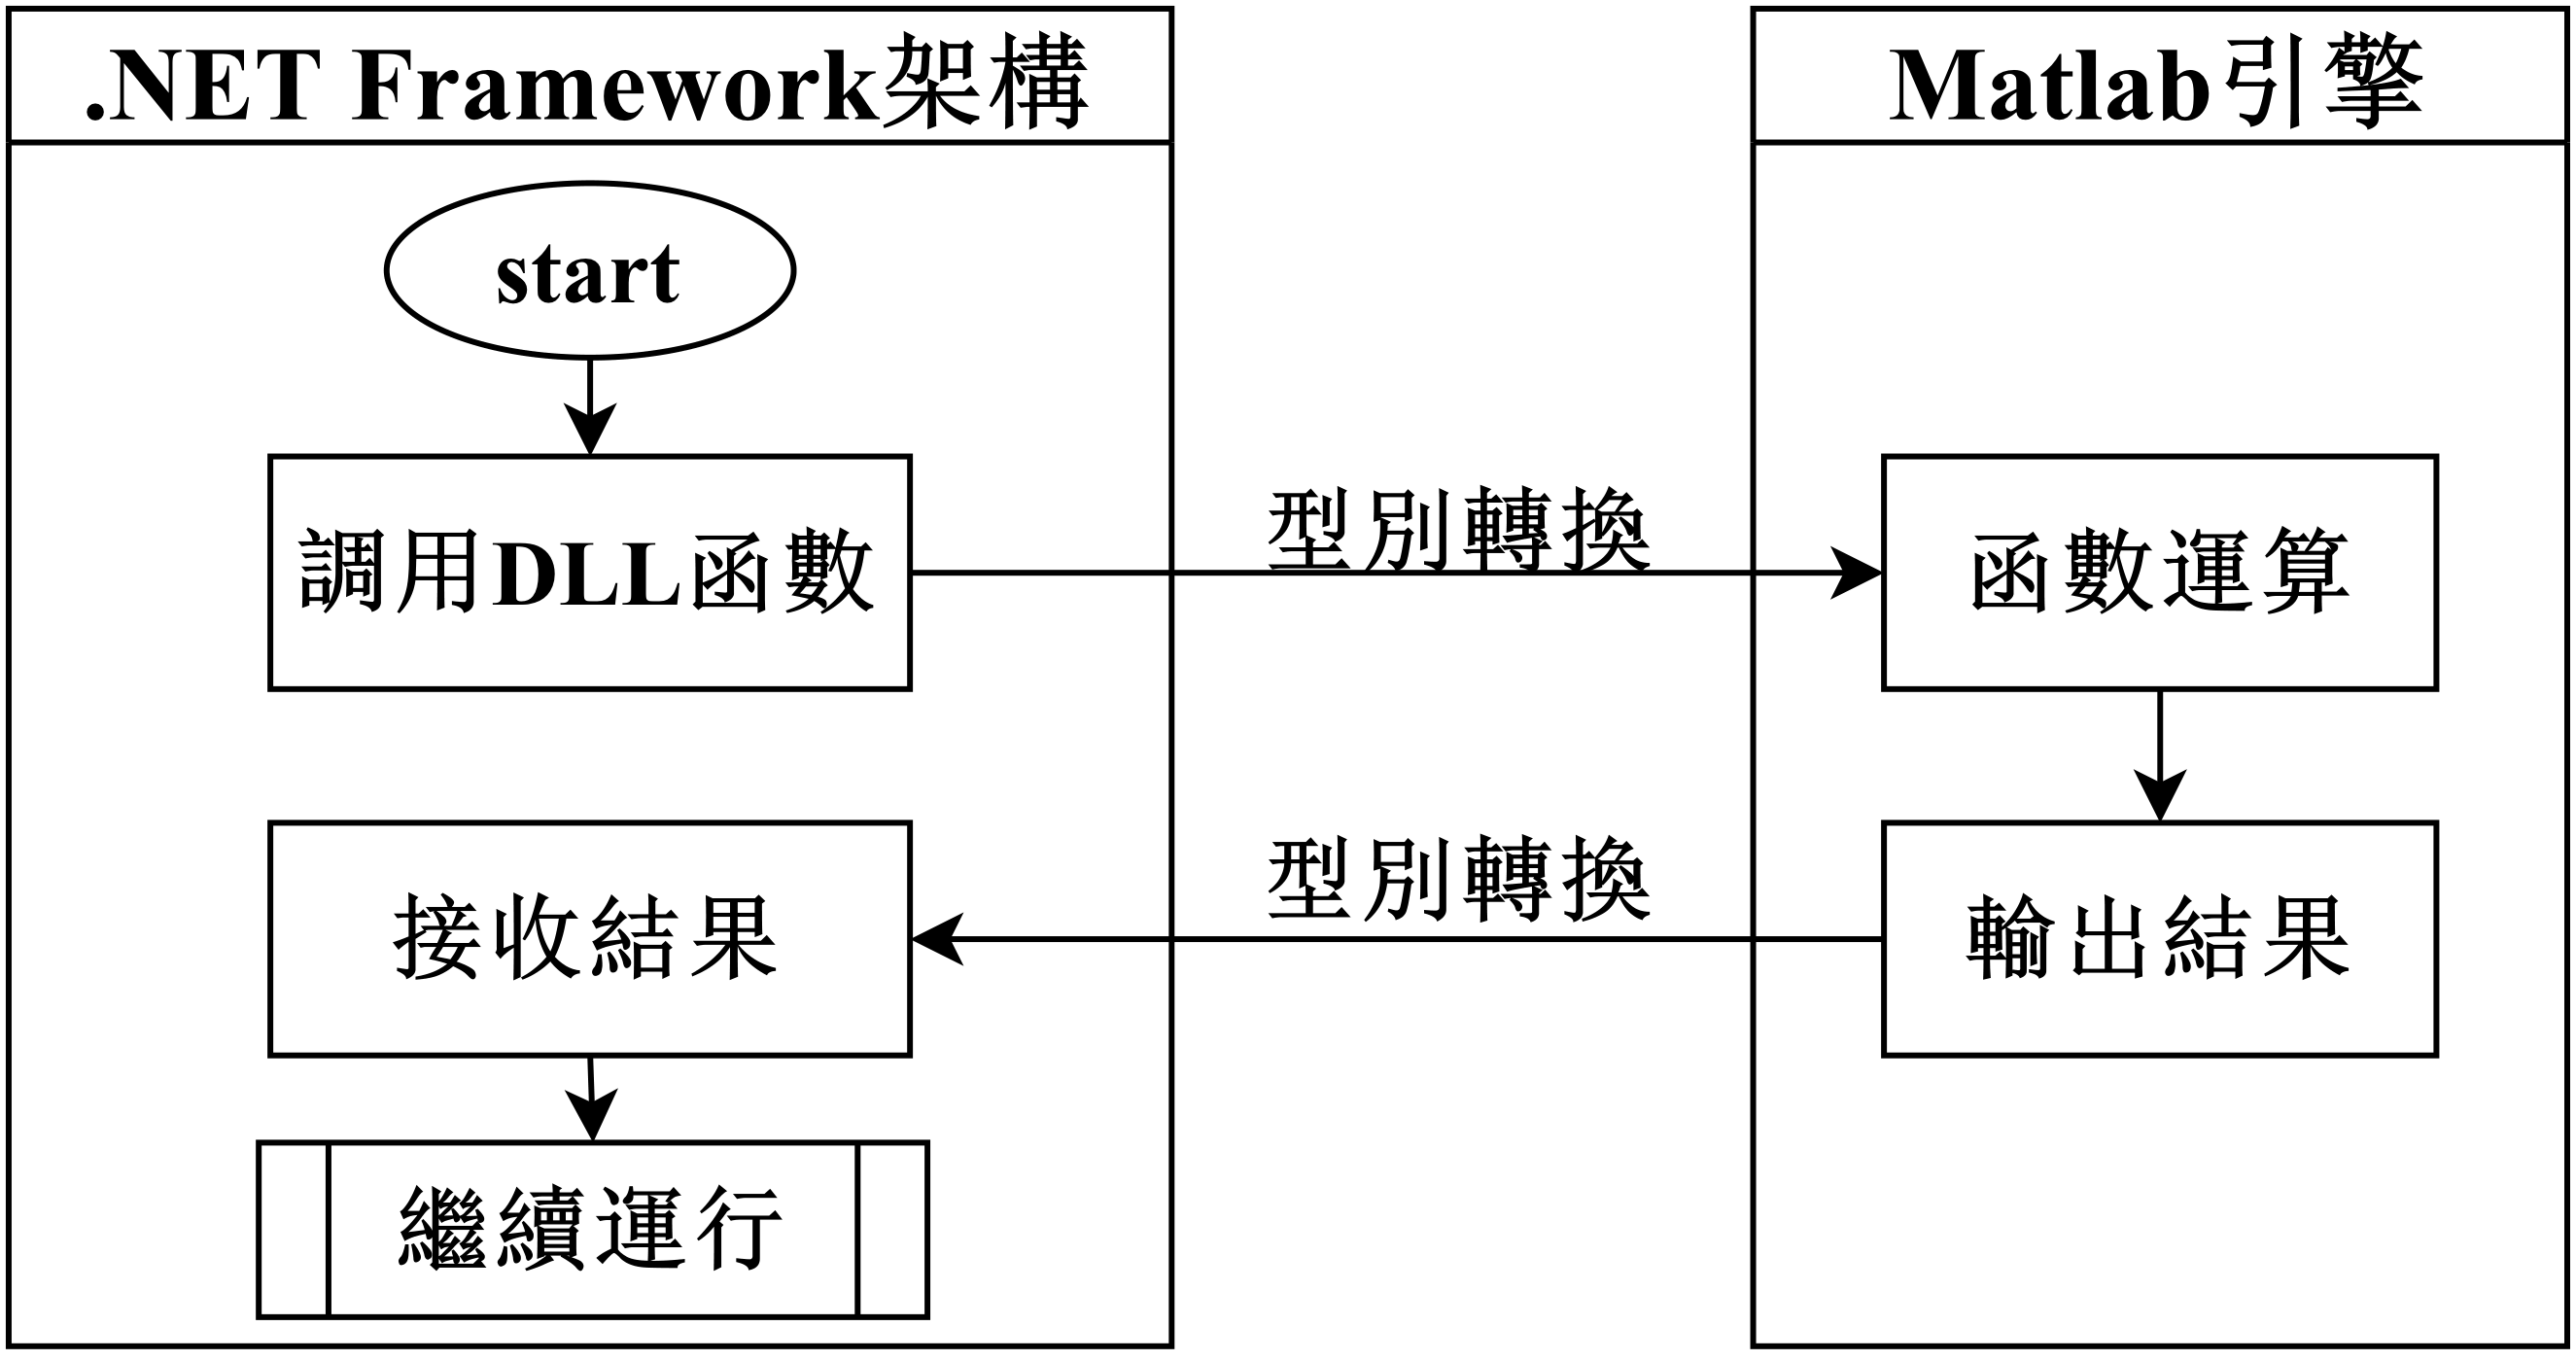
\includegraphics[width=0.8\textwidth]{figures/DLL.png} %插入图片,[]中设置图片大小,{}中是图片文件名
	\caption{DLL檔運作圖} %最终文档中希望显示的图片标题
	\label{DLL檔運作圖} %用于文内引用的标签
\end{figure}
\newpage
\begin{figure}[H] %H为当前位置,!htb为忽略美学标准,htbp为浮动图形
	\centering %图片居中
    \setlength{\abovecaptionskip}{1cm}
	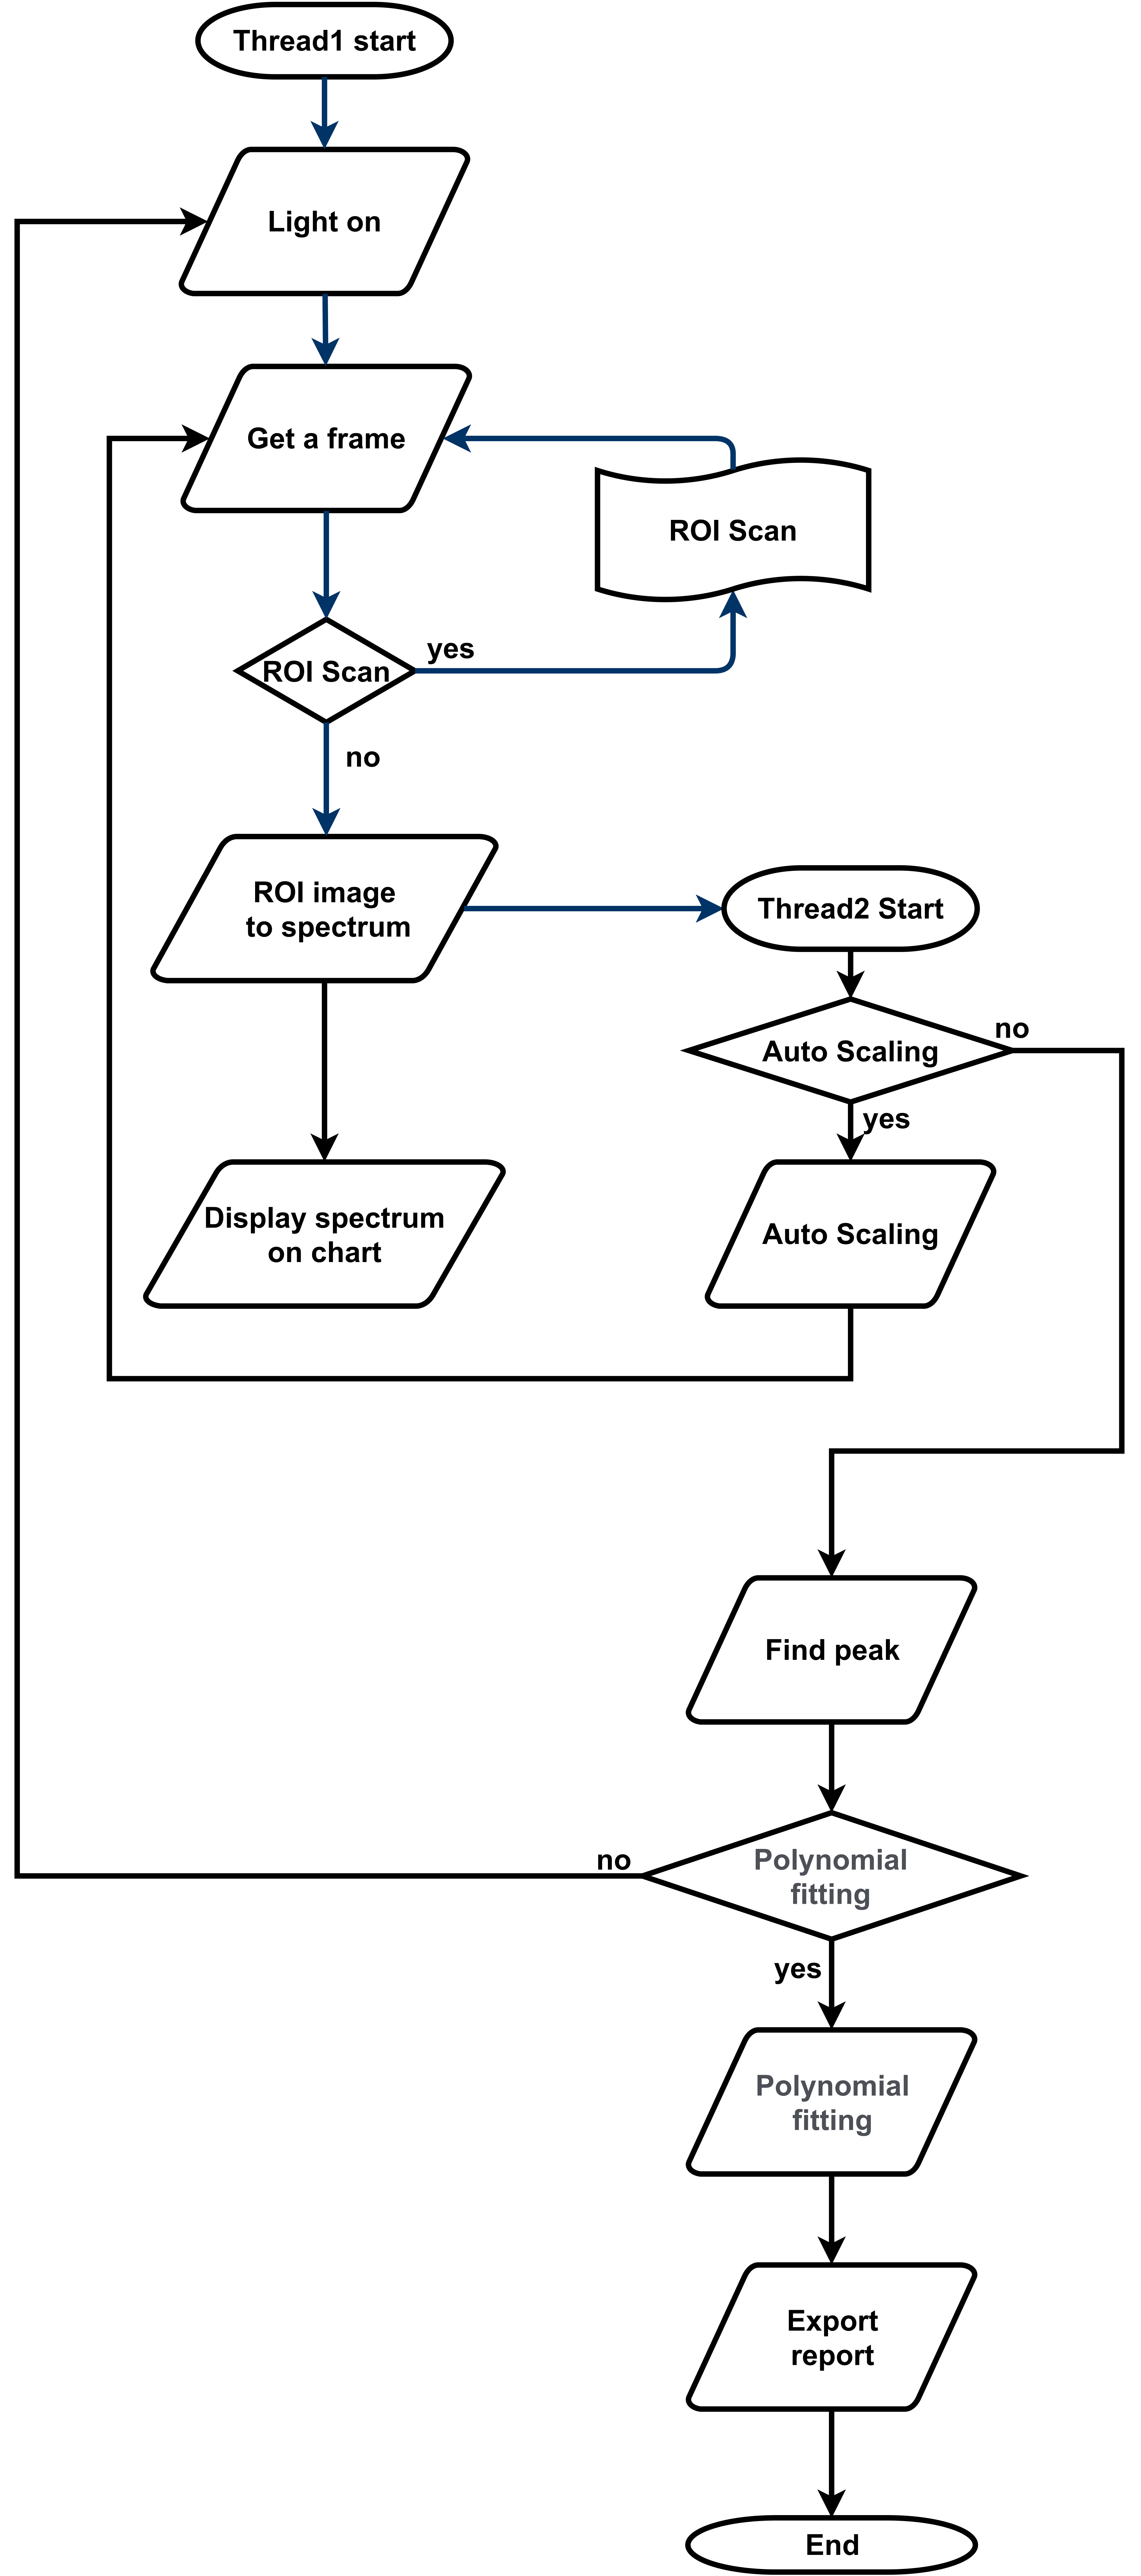
\includegraphics[width=0.6\textwidth]{figures/總流程圖.png} %插入图片,[]中设置图片大小,{}中是图片文件名
	\caption{軟體架構總流程圖} %最终文档中希望显示的图片标题
	\label{程式架構總體流程圖} %用于文内引用的标签
\end{figure}
\newpage
\section{動態連結函式庫}
動態連結函式庫(Dynamic-link library,縮寫為DLL),是為滿足使用者需要共享函式庫而由微軟在微軟視窗作業系統(Windows Form)中推出的實現方式,動態連結的意思是把時常所需要共享的的程式碼打包成DLL檔\cite{DLL},則當程式執行呼叫到DLL檔內的程式碼時,DLL可執行檔才會被系統載入到記憶體中運行,如圖\ref{DLL檔運作圖}. 所示,也因此動態連結方式僅在有需要時呼叫,可以大幅減低效能與記憶體浪費。\par
動態連結函式庫除了以上幾個主要優點外,DLL檔還能以Matlab編輯功能函數並導入其他語言架構中使用,因此在C\#語言架構下難以實現的複雜數學運算,便可以先透過Matlab建構功能函數,以達到簡化與加速複雜的演算法是本文採用動態連結函式庫的主要原因。\par
另外採用DLL檔的重要原因還有其通用性,因本研究之演算法全部皆採取Matlab編寫,而透過在Matlab中將演算法編寫成Function形式,則在打包成DLL檔後,不管在任何程式語言的架構下,只要輸入需要的輸入參數,皆可以在將資料進行型別轉換後透過DLL檔傳送給Matlab引擎進行計算,如此一來此演算法則具有良好的通用性,不管是使用C++或C語言等軟體開發時,都可以透過DLL檔使用本研究演算法。\par
由第二章使用的演算法運算過程可以看出本研究所使用的演算法需要大量的矩陣運算,因此透過DLL的方式,可由開發的C\#使用者介面,讓使用者能有簡易與美觀的操作介面,並在此建立主要的軟體架構,在此環境下所獲取的影像與資料數據,再透過型別轉換傳送至Matlab運算,經由Matlab引擎的運算可以大幅降低運算過程、所需時間與編譯複雜度,完成運算後的結果再經過資料型別轉換後傳送回原本的軟體架構中,如此一來便可以同時維持軟體的美觀與使用者操作體驗,並且可以進行相當複雜的運算,而且不需提高運算時間與編寫的複雜度。
\section{ROI Scan}
在進行影像與光譜之間的轉換之前,ROI Scan是必經的重要步驟之一。當一影像經由影像感測器取出,若將影像以矩陣方式表示如式(\ref{eq3.1}),則座標原點落於影像的最左上點即(x = 0, y = 0),其中x座標往右為正、y座標往下為正,如圖\ref{全幅雷射光譜影像}. 所示。
\begin{equation}\label{eq3.1}
	\begin{bmatrix} 
		(0,0)&(1,0)&\cdots&(1278,0)&(1279,0)\\
		(0,1)&(1,1)&\cdots&(1278,1)&(1279,1)\\
		(0,2)&(1,2)&\cdots&(1278,2)&(1279,2)\\
		\vdots&\vdots&\ddots&\vdots&\vdots\\
		(0,957)&(1,957)&\cdots&(1278,957)&(1279,957)\\
		(0,958)&(1,958)&\cdots&(1278,958)&(1279,958)\\
		(0,959)&(1,959)&\cdots&(1278,959)&(1279,959)\\
	\end{bmatrix}_{960\times1280}
\end{equation}
\par
設定ROI為長1280pixel、寬20pixel的矩形,將此矩形置於矩陣(\ref{eq3.1}),由上至下掃描,以矩陣表示為矩陣(\ref{eq3.2})形式,並且將ROI矩形內所有像素的強度(Intensity)總和紀錄於記憶體(Memory)中,最後判定強度總和最大的矩形位置即為影像的ROI。
\begin{equation}\label{eq3.2}
	\begin{bmatrix} 
		(x_{i},y_{i})&(x_{i+1},y_{i})&\cdots&(x_{i+1278},y_{i})&(x_{i+1279},y_{i})\\
		(x_{i},y_{i+1})&(x_{i+1},y_{i+1})&\cdots&(x_{i+1278},y_{i+1})&(x_{i+1279},y_{i+1})\\
		\vdots&\vdots&\ddots&\vdots&\vdots\\
		(x_{i},y_{i+18})&(x_{i+1},y_{i+18})&\cdots&(x_{i+1278},y_{i+18})&(x_{i+1279},y_{i+18})\\
		(x_{i},y_{i+19})&(x_{i+1},y_{i+19})&\cdots&(x_{i+1278},y_{i+19})&(x_{i+1279},y_{i+19})\\
	\end{bmatrix}_{20\times1280}
\end{equation}
\section{ROI影像轉換光譜}
進行光譜分析前,如何將一全幅光譜影像轉換為光譜波形,是最基本且必要的步驟之一,當一全幅雷射光譜影像由影像感測器取出如圖\ref{全幅雷射光譜影像}. 所示。
\begin{figure}[H] %H为当前位置,!htb为忽略美学标准,htbp为浮动图形
	\centering %图片居中
	\vspace{0.8cm}
	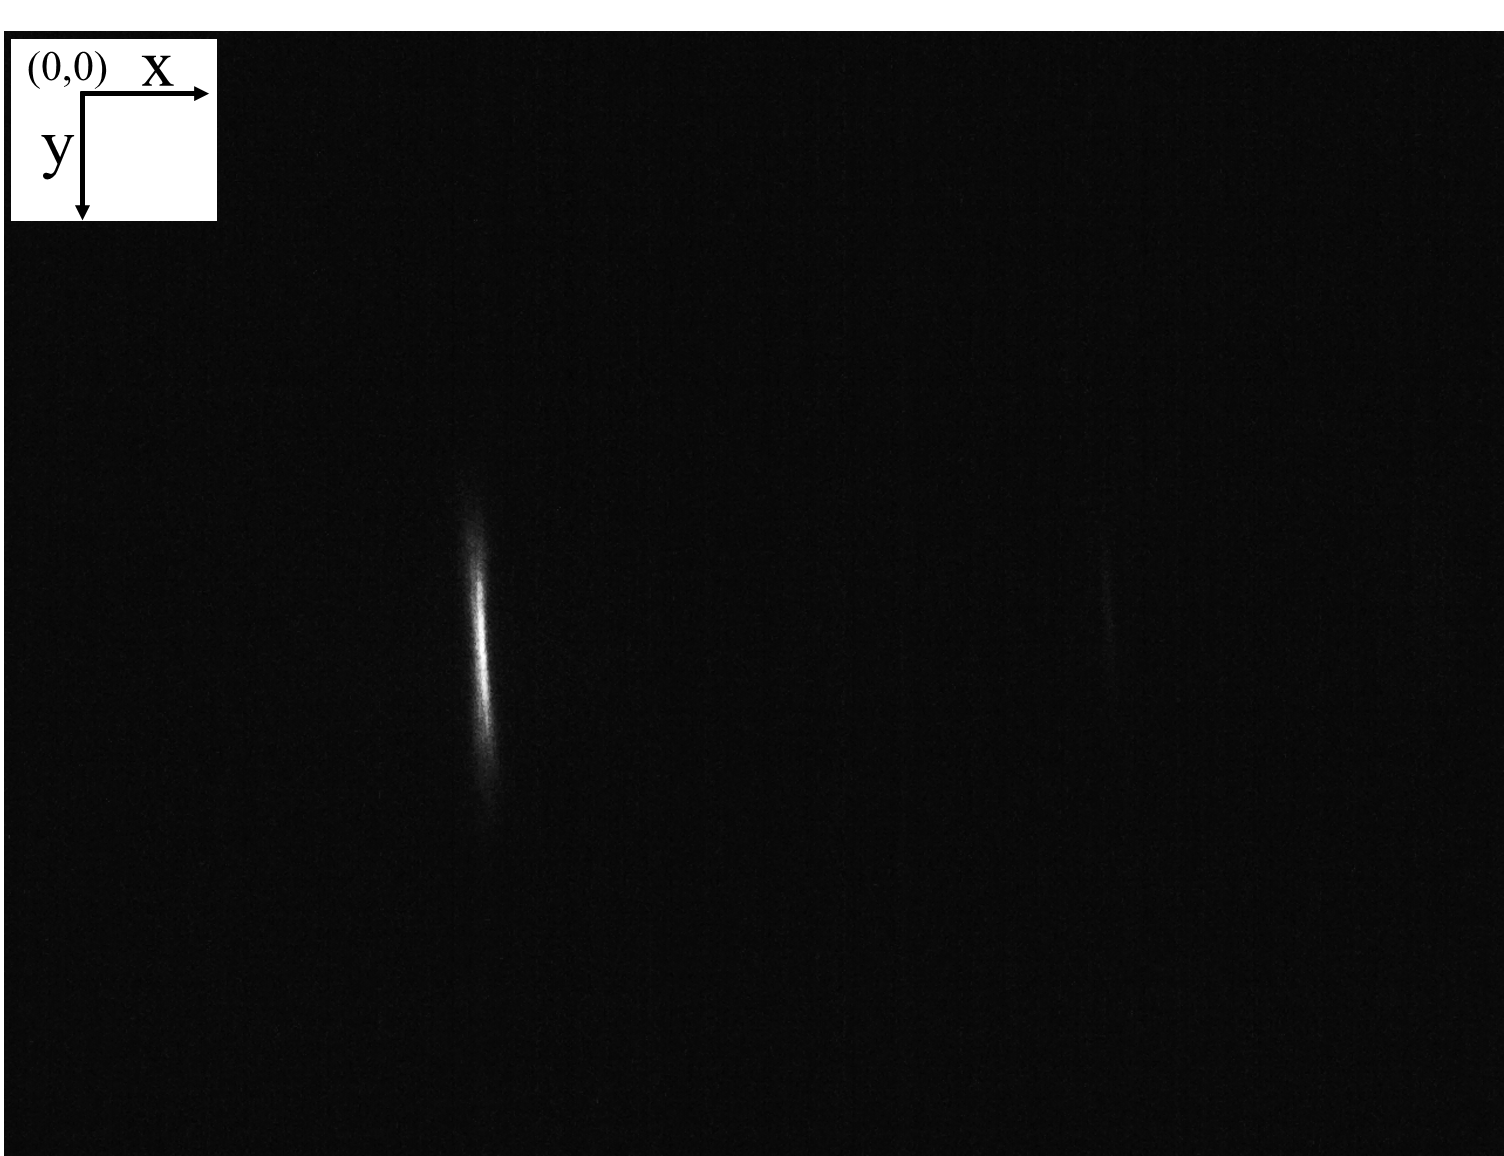
\includegraphics[width=13cm]{figures/TEST_0303_Image__Laser2_2021-03-03-14-23-20.png} %插入图片,[]中设置图片大小,{}中是图片文件名
	\caption{全幅雷射光譜影像} %最终文档中希望显示的图片标题
	\label{全幅雷射光譜影像} %用于文内引用的标签
\end{figure}
若將圖\ref{全幅雷射光譜影像}. 每一個像素皆轉換成光譜訊息,將需要大量的運算,並且在感測器發生漏光(圖\ref{漏光光譜影像}. )時,將會造成光譜波形起始處因漏光而波形失真(圖\ref{漏光時全幅影像光譜波形圖}. ),因此需先由3.3章ROI Scan方式找出全幅影像的ROI區間(圖\ref{全幅雷射ROI光譜影像}. ),以大幅降低運算量,且降低漏光等環境光因素造成的影響。
\begin{figure}[H] %H为当前位置,!htb为忽略美学标准,htbp为浮动图形
	\centering %图片居中
	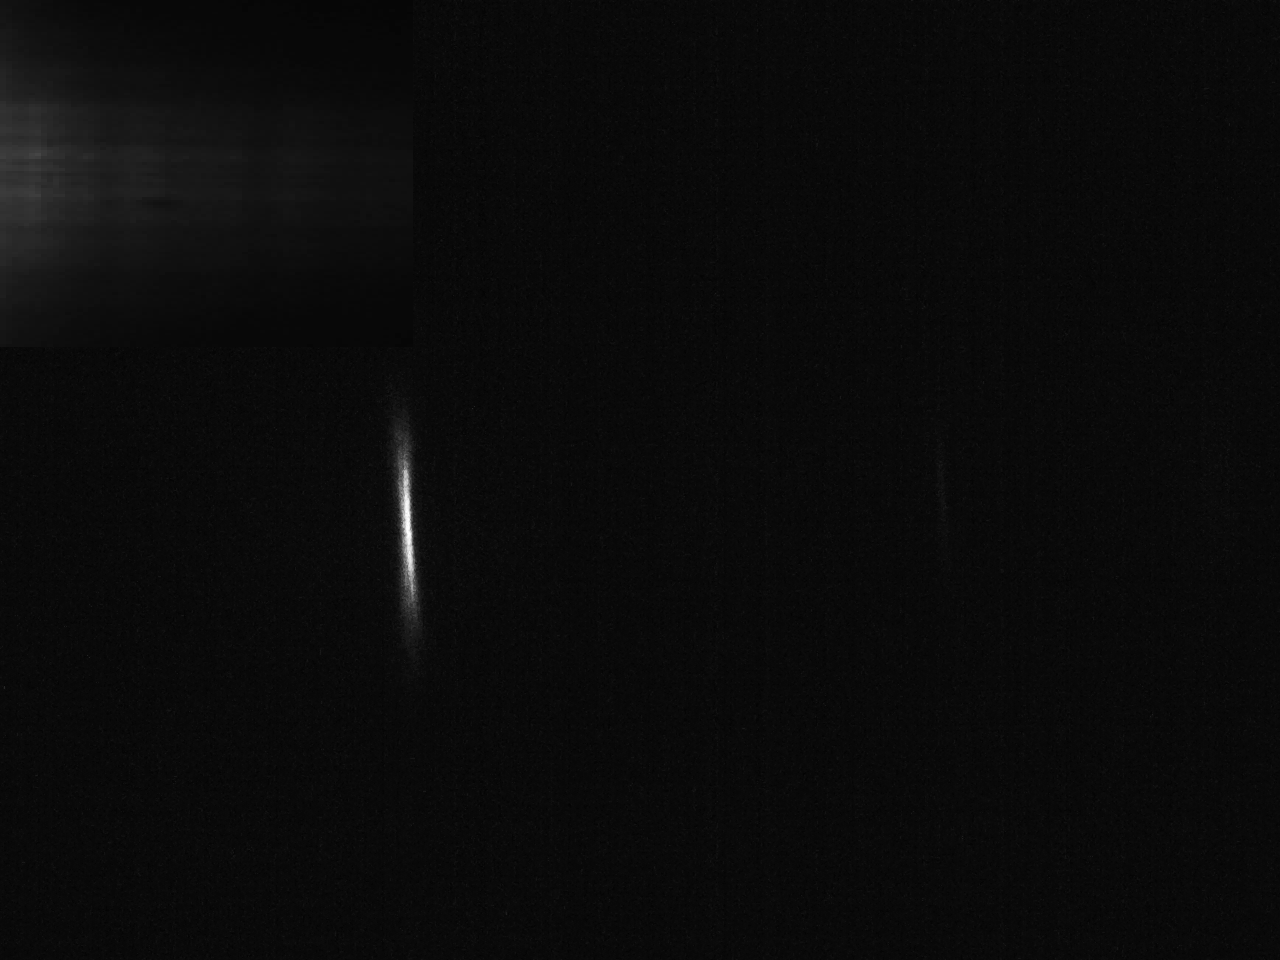
\includegraphics[width=13cm]{figures/漏光影像.png} %插入图片,[]中设置图片大小,{}中是图片文件名
	\caption{漏光光譜影像} %最终文档中希望显示的图片标题
	\label{漏光光譜影像} %用于文内引用的标签
\end{figure}
\begin{figure}[H] %H为当前位置,!htb为忽略美学标准,htbp为浮动图形
	\centering %图片居中
	\setlength{\abovecaptionskip}{0.cm}
	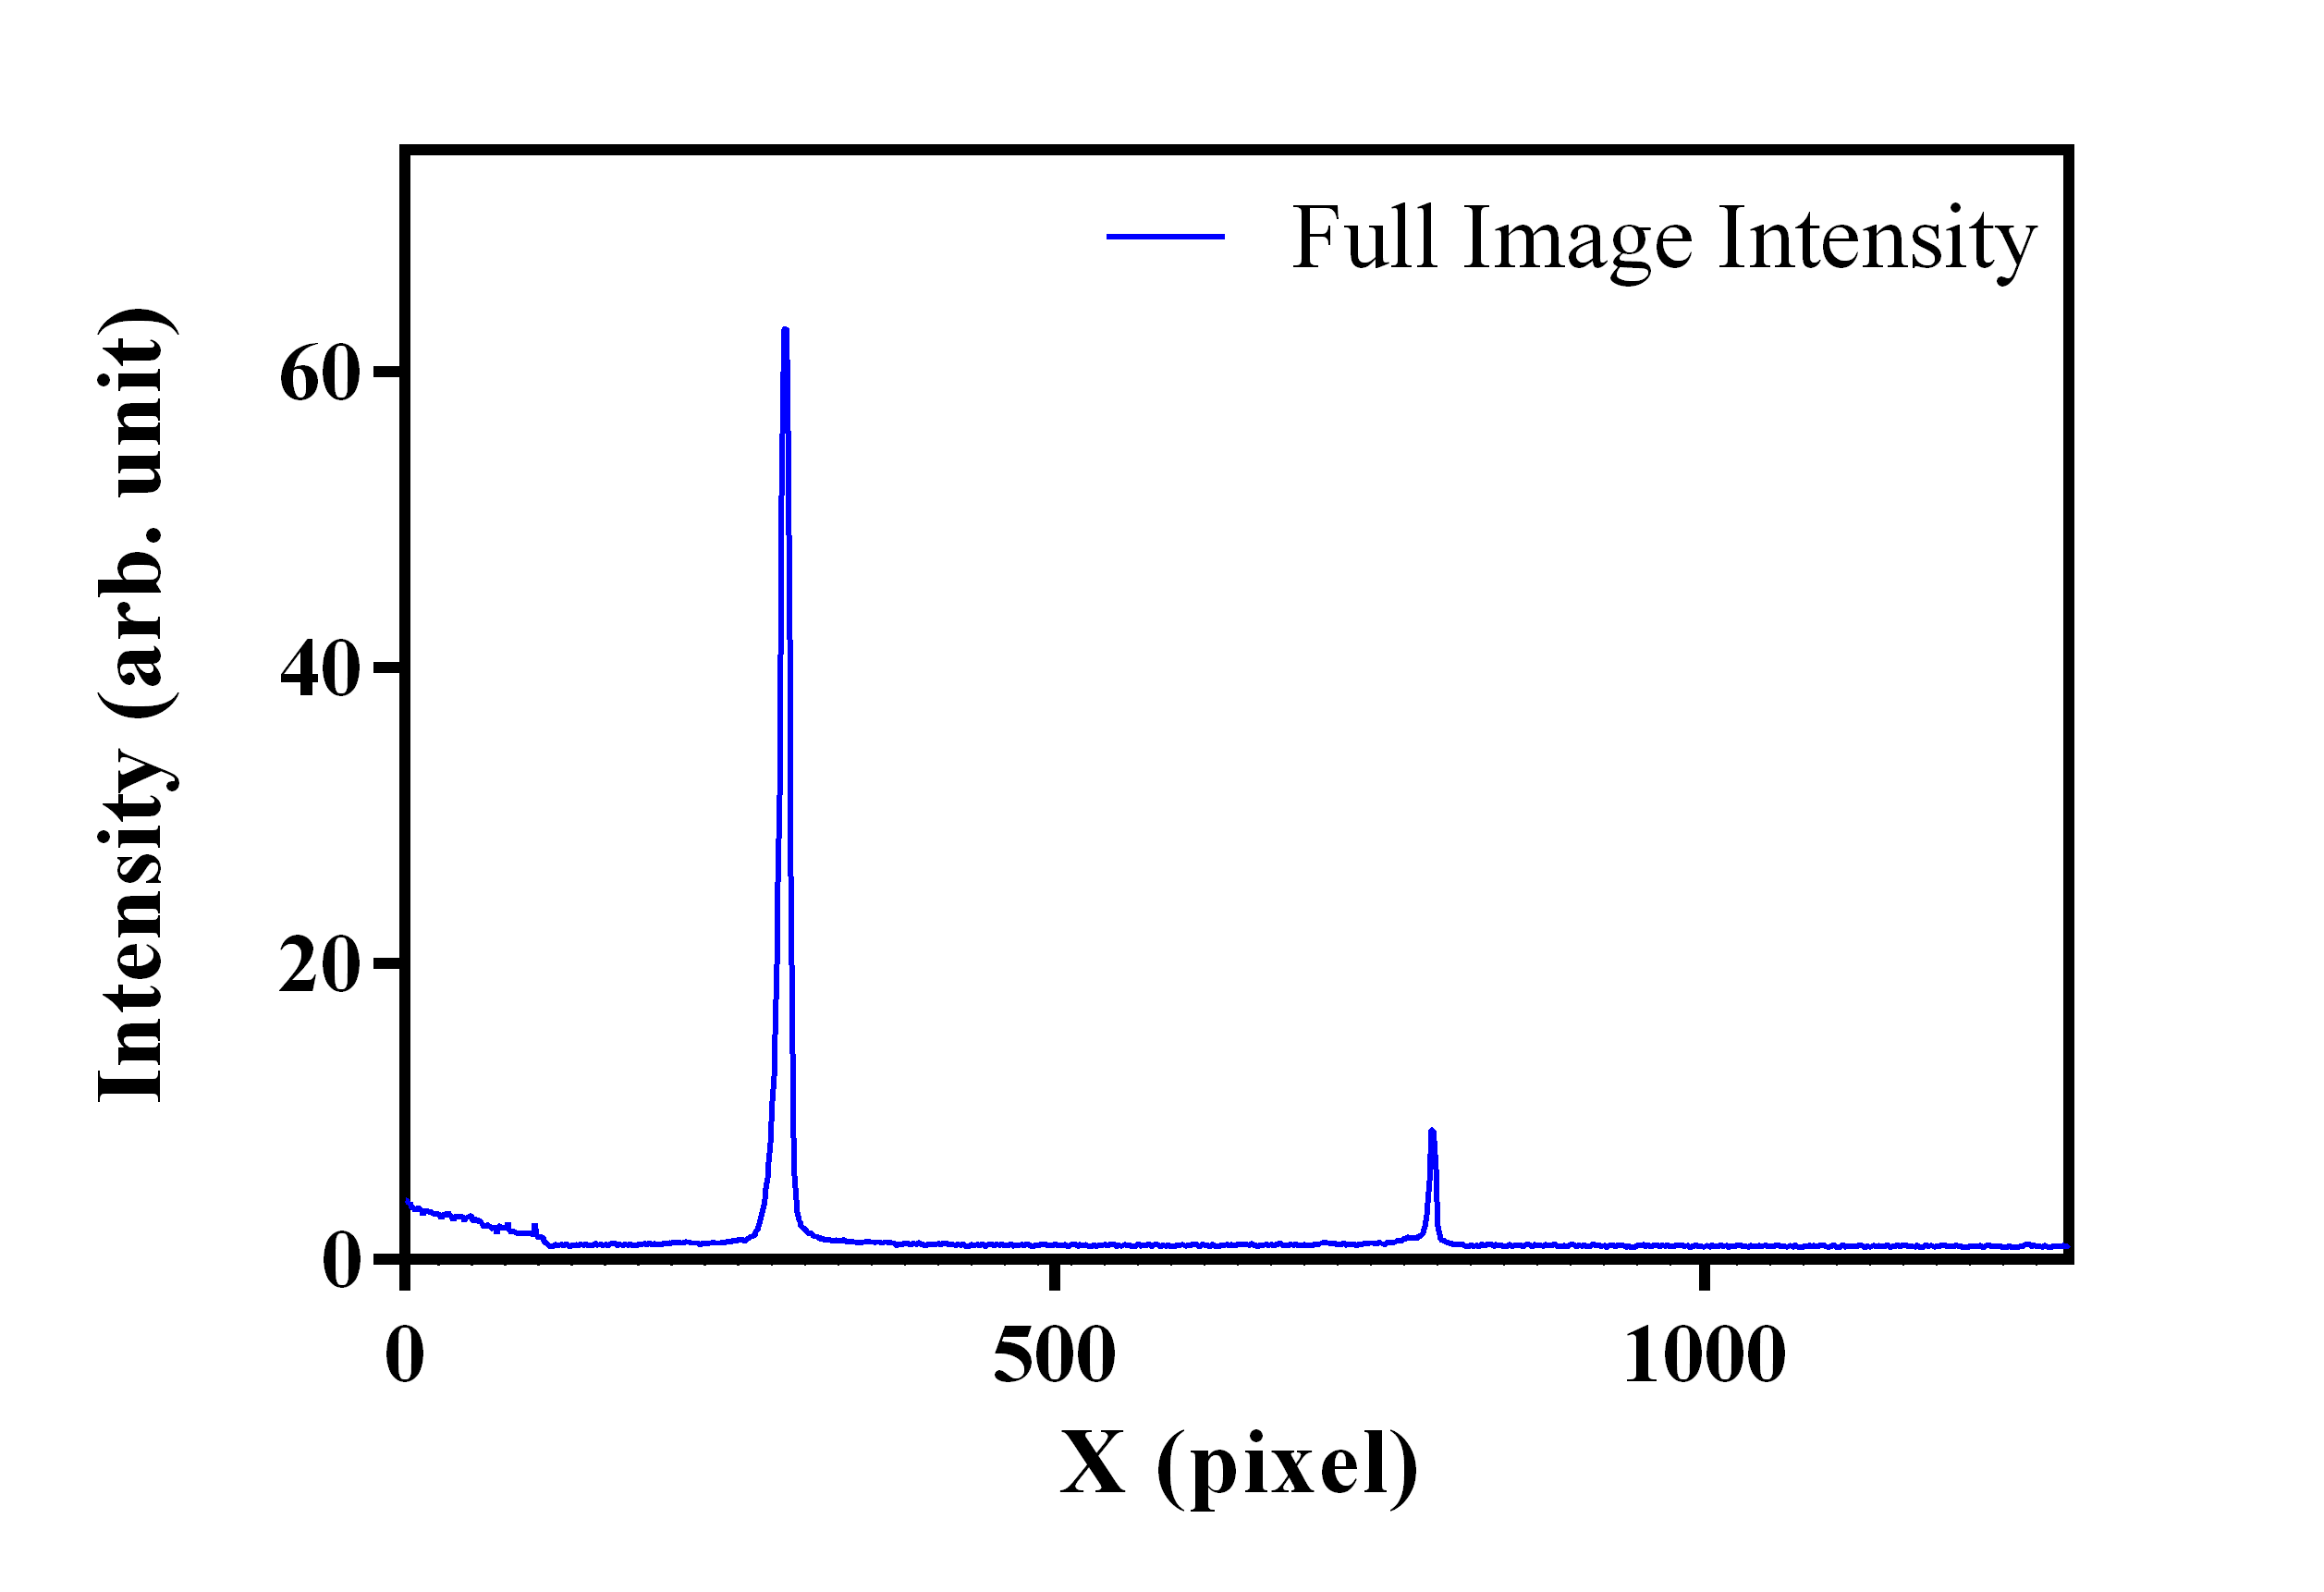
\includegraphics[width=15cm]{figures/MissLight.png} %插入图片,[]中设置图片大小,{}中是图片文件名
	\caption{漏光時全幅影像光譜波形圖} %最终文档中希望显示的图片标题
	\label{漏光時全幅影像光譜波形圖} %用于文内引用的标签
\end{figure}
\begin{figure}[H] %H为当前位置,!htb为忽略美学标准,htbp为浮动图形
	\centering %图片居中
	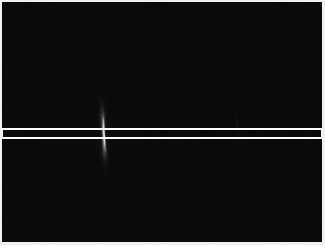
\includegraphics[width=10cm]{figures/TEST_0303_full_Image__Laser2_2021-03-03-14-23.jpg} %插入图片,[]中设置图片大小,{}中是图片文件名
	\caption{全幅雷射ROI光譜影像} %最终文档中希望显示的图片标题
	\label{全幅雷射ROI光譜影像} %用于文内引用的标签
\end{figure}
得出ROI區域後,將ROI區間的影像由全幅雷射光譜影像中單獨取出分析,如圖\ref{ROI光譜影像}. 所示。
\begin{figure}[H] %H为当前位置,!htb为忽略美学标准,htbp为浮动图形
	\centering %图片居中
	\vspace{0.8cm}
	
\includegraphics[width=13cm]{figures/TEST_0303_ROI__Laser2_2021-03-03-14-23-20.jpg} %插入图片,[]中设置图片大小,{}中是图片文件名
	\caption{ROI光譜影像} %最终文档中希望显示的图片标题
	\label{ROI光譜影像} %用于文内引用的标签
\end{figure}
影像感測器所取出之原始光譜影像為三通道RGB影像,透過2.1章的RBG轉換式(\ref{eq:2.4})將ROI光譜影像中每一個像素的RGB值,透過灰度轉換公式轉換成灰度值,比如影像在$Pixel(400,520)$位置的RGB值為$(174,156,148)$,以$RGB(400,520)=(174,156,148)$表示並帶入式(\ref{eq:2.4})。
\begin{equation}
	Gray(400,520) = (174\times313524 + 156\times615514 + 148\times119538) >> 20
	\label{RGB:3.3}
\end{equation}
其中$Gray(400,520)$為在$Pixel(400,520)$的灰度值表示,計算後為
\begin{equation}
	Gray(400,520) = 168264984_{(10)} >> 20
	\label{RGB:3.4}
\end{equation}
再將十進制灰度值轉換為二進制
\begin{equation}
	Gray(400,520) = 1010000001111000010100011000_{(2)} >> 20
	\label{RGB:3.5}
\end{equation}
再對二進制灰度值像右位移20個位元,得
\begin{equation}
	Gray(400,520) = 10100000_{(2)}
	\label{RGB:3.6}
\end{equation}
最後轉回十進制
\begin{equation}
	Gray(400,520) = 160_{(10)}
	\label{RGB:3.7}
\end{equation}
將ROI中所有像素如式(\ref{RGB:3.3})至式(\ref{RGB:3.7})逐一帶入,則得出影像每一像素之灰度值,將ROI影像以灰度值矩陣表示。
\begin{equation}\label{RGB:3.8}
	\begin{bmatrix} 
		G(0,0)&G(1,0)&\cdots&G(1278,0)&G(1279,0)\\
		G(0,1)&G(1,1)&\cdots&G(1278,1)&G(1279,1)\\
		\vdots&\vdots&\ddots&\vdots&\vdots\\
		G(0,18)&G(1,18)&\cdots&G(1278,18)&G(1279,18)\\
		G(0,19)&G(1,19)&\cdots&G(1279,19)&G(1279,19)\\
	\end{bmatrix}_{20\times1280}
\end{equation}
矩陣對每一行各自取灰度值平均,則得出像素對光度數據矩陣。
\begin{equation}\label{RGB:3.9}
	\begin{bmatrix} 
		\frac{\Sigma_{i=0}^{i=19}G(0,i)}{20}&\frac{\Sigma_{i=0}^{i=19}G(1,i)}{20}&\cdots&\frac{\Sigma_{i=0}^{i=19}G(1278,i)}{20}&\frac{\Sigma_{i=0}^{i=19}G(1279,i)}{20}\\
	\end{bmatrix}_{1\times1280}
\end{equation}
式(\ref{RGB:3.9})中$1\times1280$之矩陣即為光譜數據矩陣,其中每一像素對應一個光度值,轉換完成後的光譜波形圖如圖\ref{ROI光譜強度圖}. 所示。
\begin{figure}[H] %H为当前位置,!htb为忽略美学标准,htbp为浮动图形
	\centering %图片居中
	\setlength{\abovecaptionskip}{0.cm}
	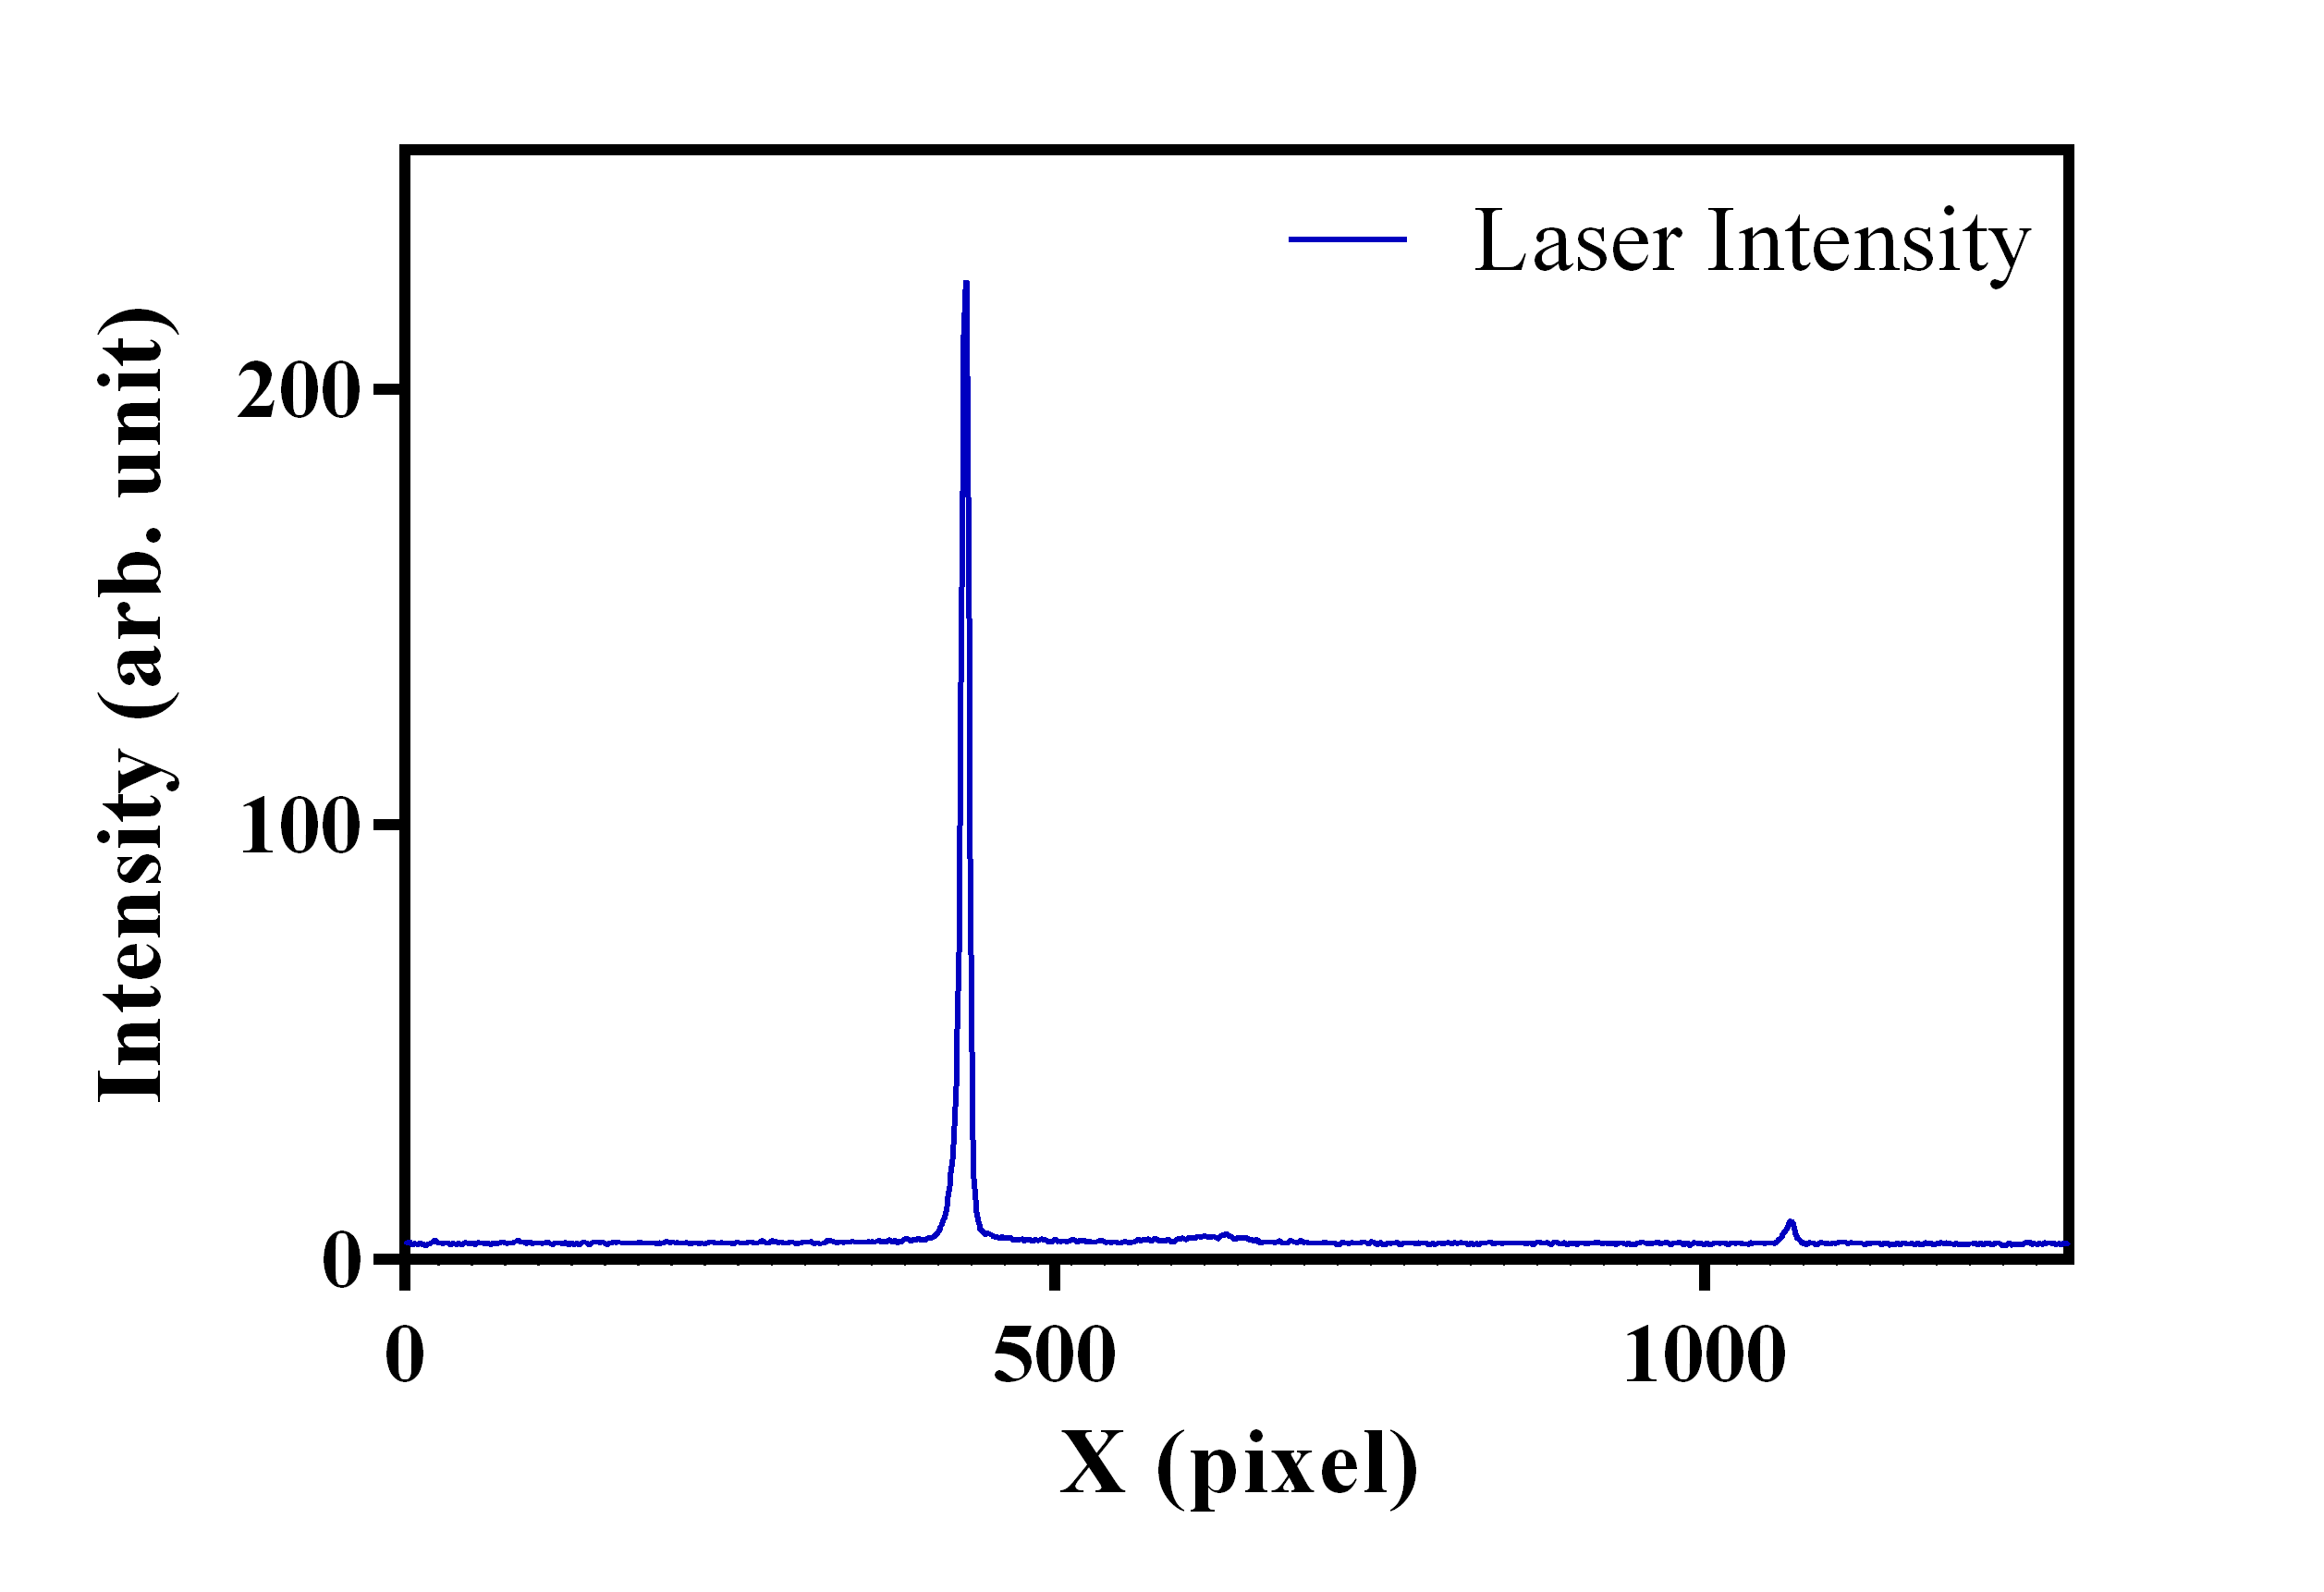
\includegraphics[width=\textwidth]{figures/Laser_Intensity.PNG} %插入图片,[]中设置图片大小,{}中是图片文件名
	\caption{ROI光譜強度圖} %最终文档中希望显示的图片标题
	\label{ROI光譜強度圖} %用于文内引用的标签
\end{figure}
\section{Auto Scaling}
取得光譜波形資訊後,並無法立即進行分析,因受限於灰度強度最高值255,當光線強度過強而超出255時即稱為過瞨\cite{over-exposure},光譜過曝如圖\ref{白光光譜過瞨圖}. 所示,波峰位置將難以辨認,因此需調低影像感測器參數,以獲得較低的光譜影像,直至總光譜的最大強度值達到目標強度為止,而當輸入波形因晶片效率較差或光源較暗,而導致強度過低如圖\ref{白光光譜強度過低圖}. 所示,則需調高影像感測器參數,直至獲得強度為目標強度為止,而上述步驟統稱為Auto Scaling,Auto Scaling結束的光譜波形表現如圖\ref{白光光譜經Auto Scaling後光譜波形表現}. 所示,強度調整至約由使用者設定的255的90\%,此光譜波形將比起未Auto Scaling來的容易分析許多。
\newpage
\begin{figure}[H] %H为当前位置,!htb为忽略美学标准,htbp为浮动图形
	\centering %图片居中
	\setlength{\abovecaptionskip}{0.cm}
	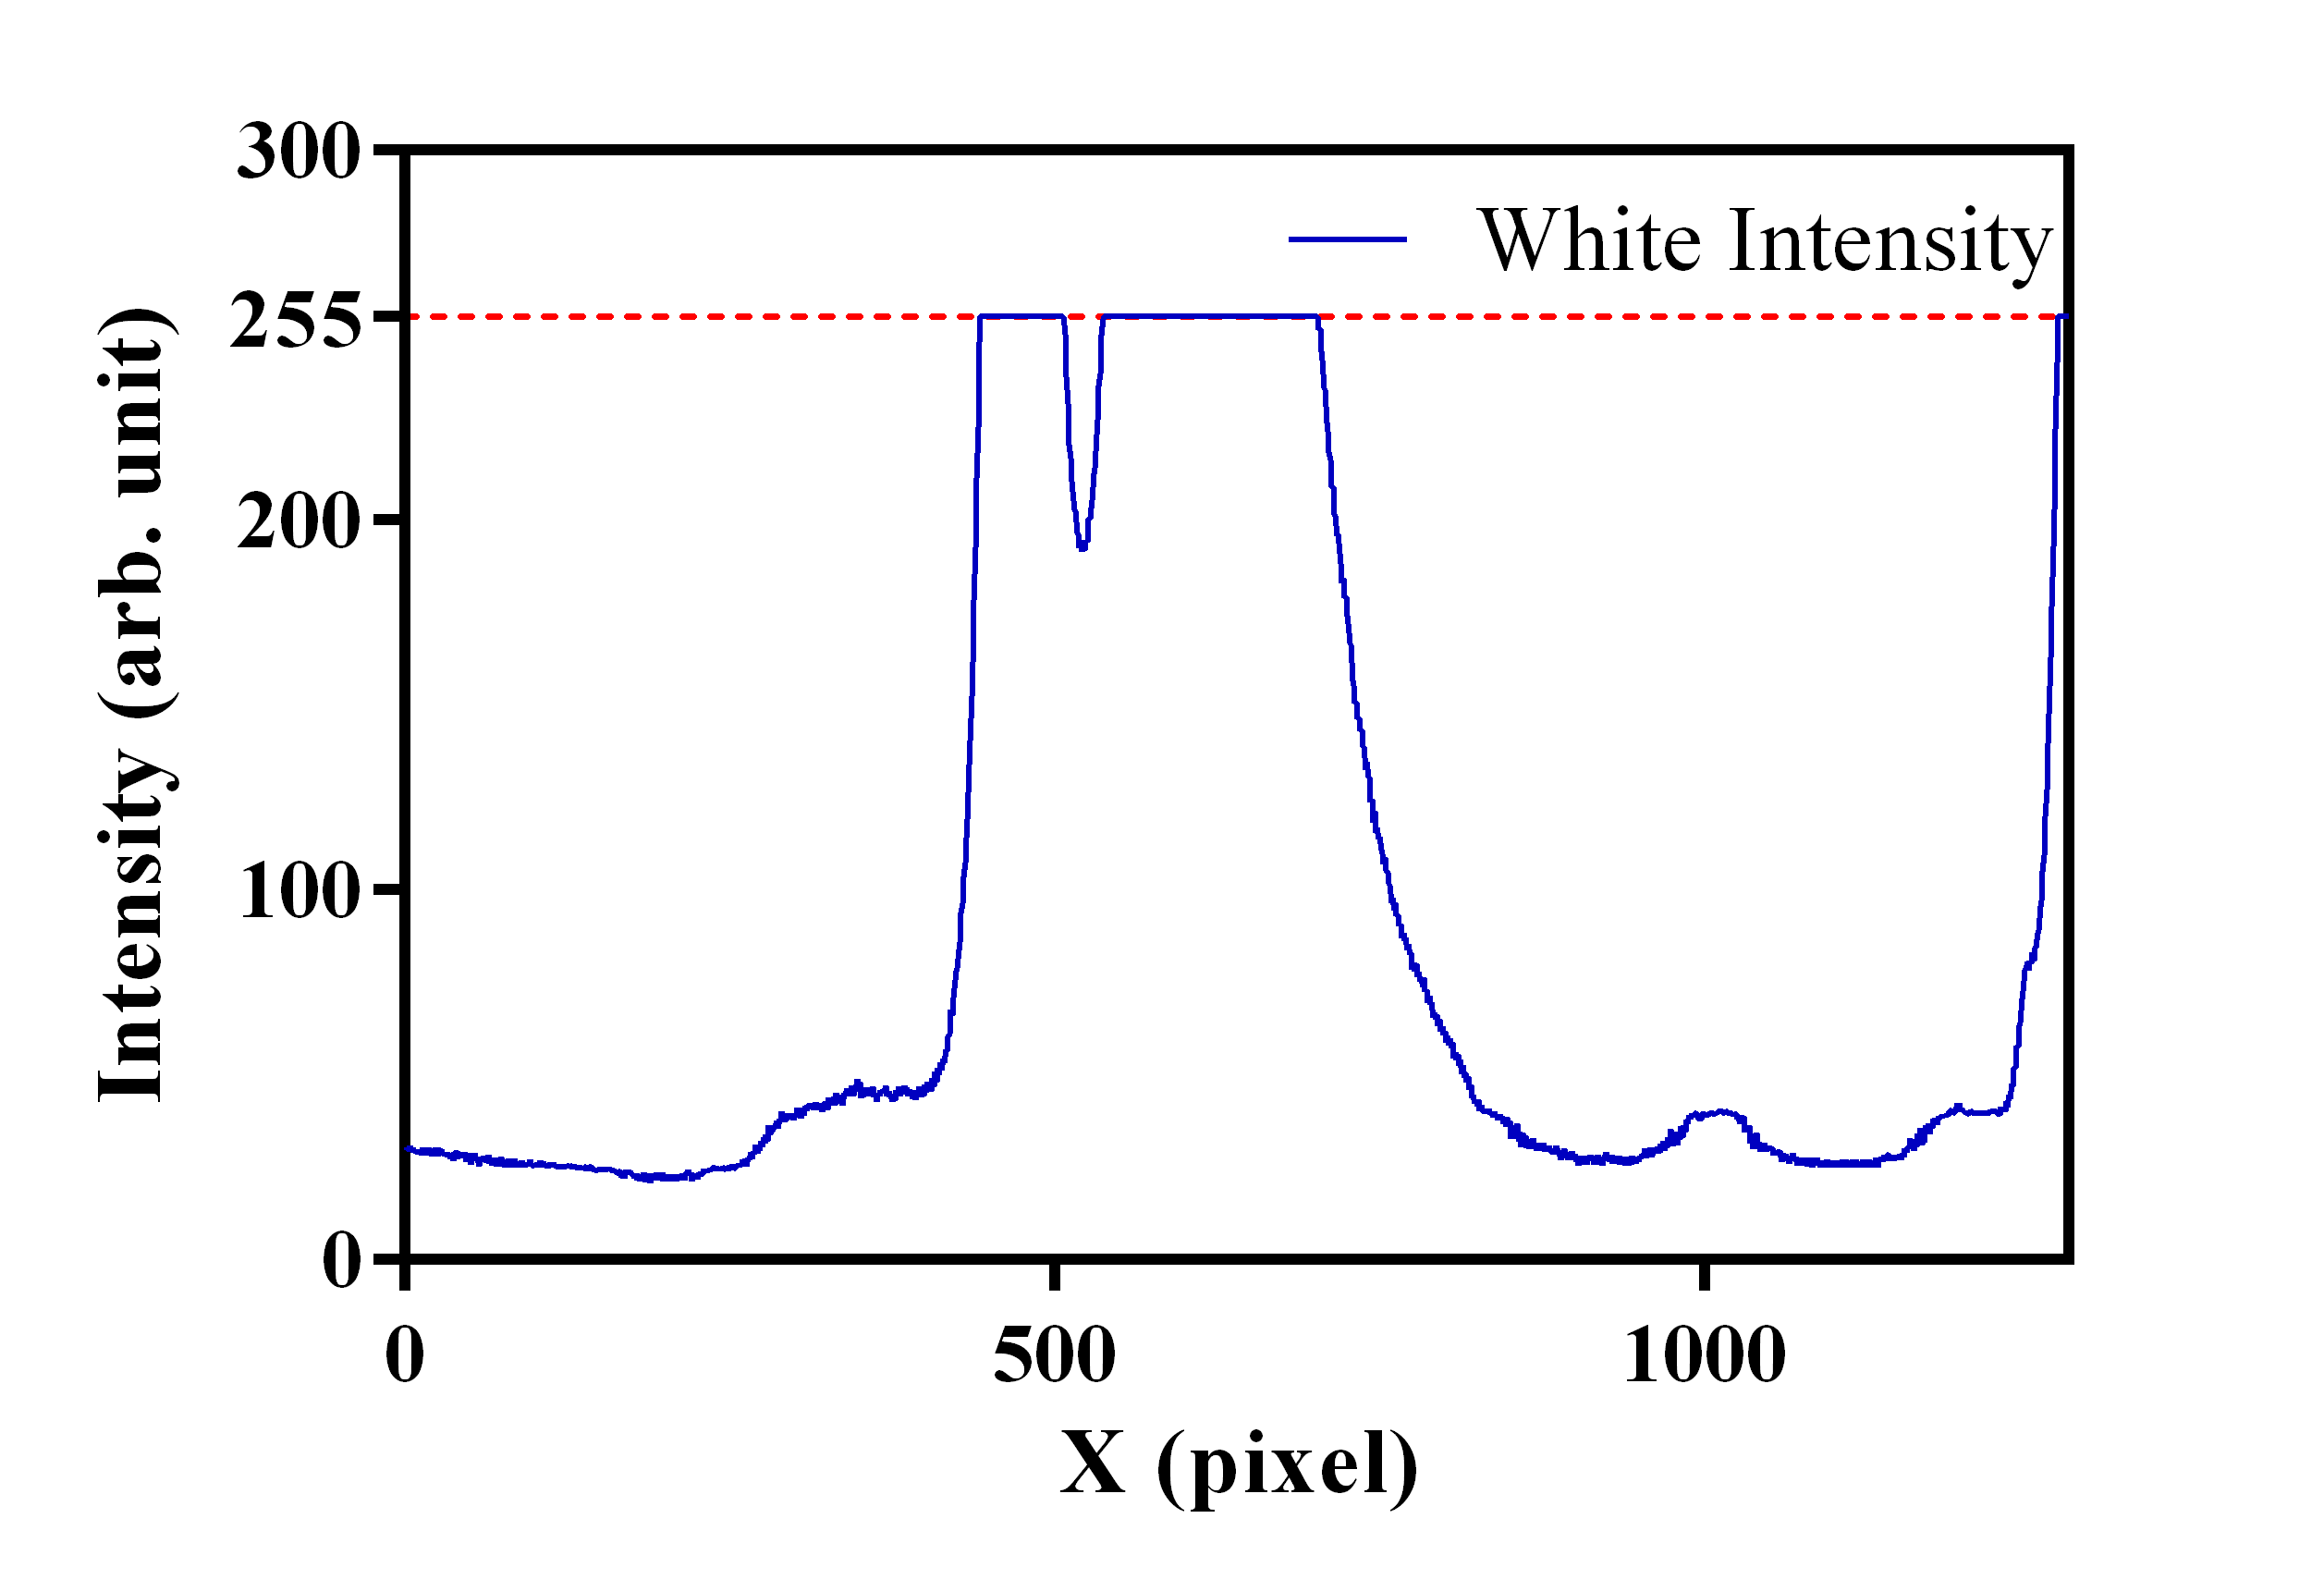
\includegraphics[width=\textwidth]{figures/White_Over.PNG} %插入图片,[]中设置图片大小,{}中是图片文件名
	\caption{白光光譜過瞨圖} %最终文档中希望显示的图片标题
	\label{白光光譜過瞨圖} %用于文内引用的标签
\end{figure}
\begin{figure}[H] %H为当前位置,!htb为忽略美学标准,htbp为浮动图形
	\centering %图片居中
	\setlength{\belowcaptionskip}{-1cm} 
	\setlength{\abovecaptionskip}{0.cm}
	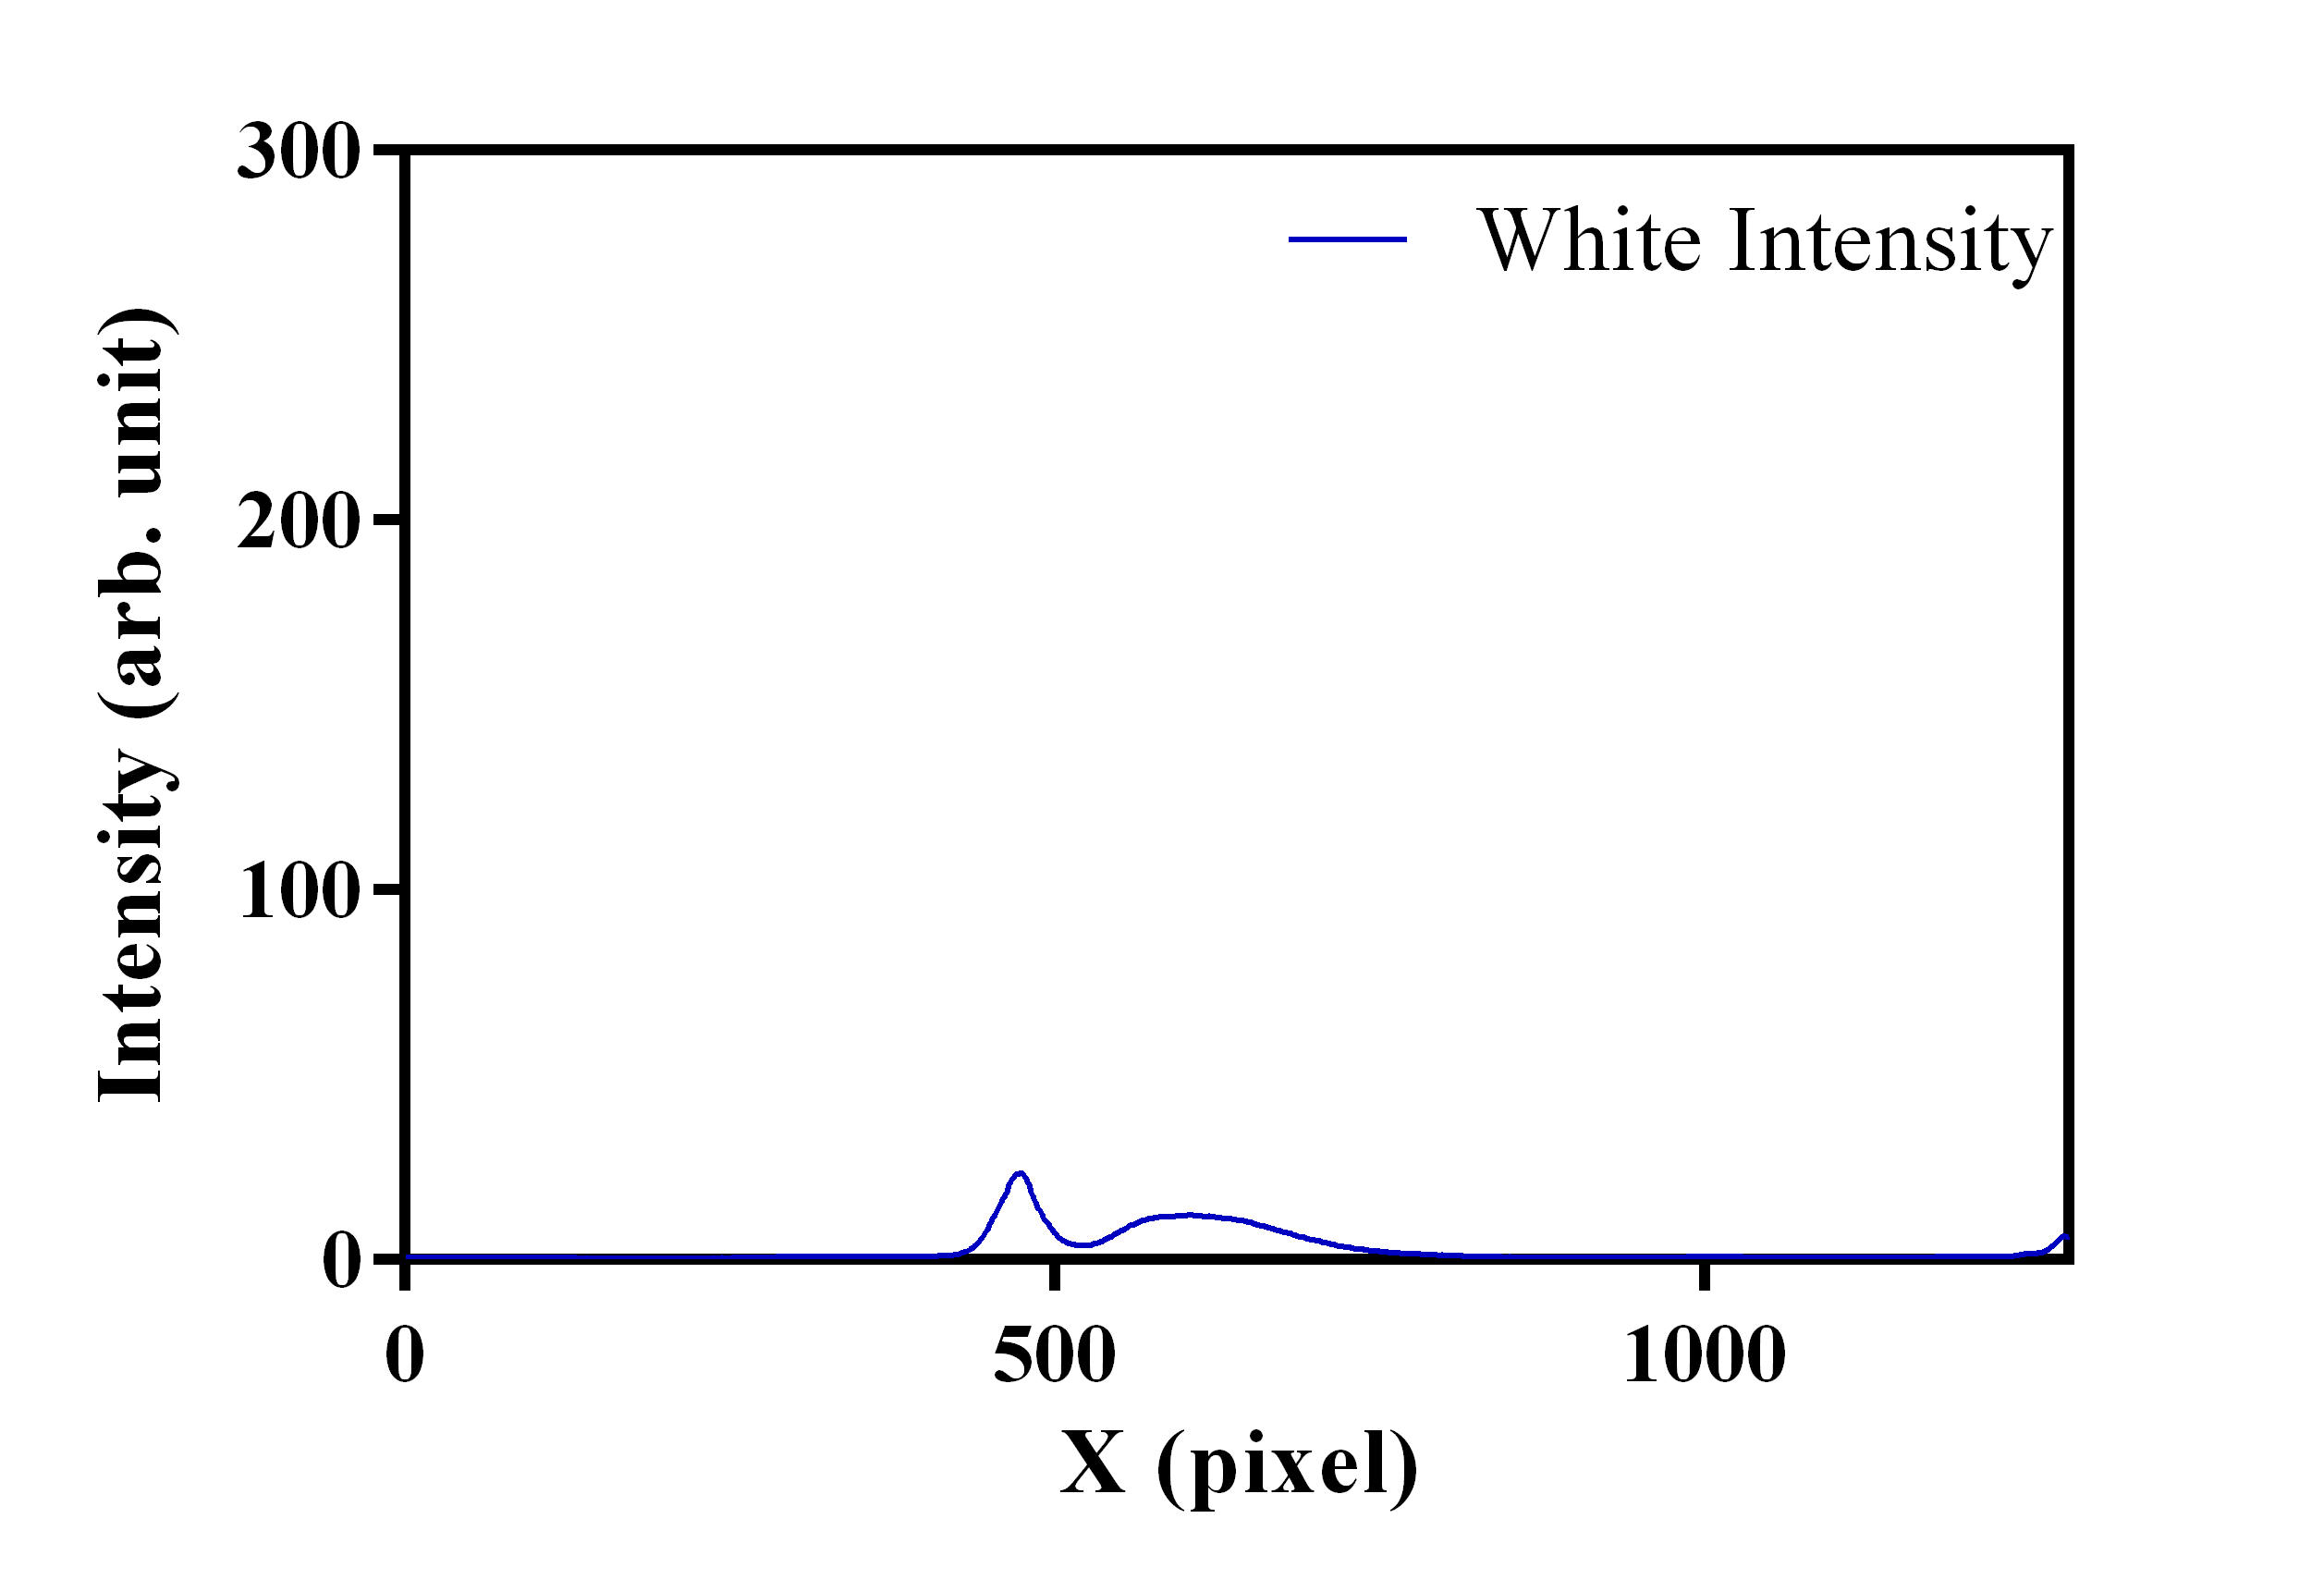
\includegraphics[width=\textwidth]{figures/White_weak.PNG} %插入图片,[]中设置图片大小,{}中是图片文件名
	\caption{白光光譜強度過低圖} %最终文档中希望显示的图片标题
	\label{白光光譜強度過低圖} %用于文内引用的标签
\end{figure}\newpage
\begin{figure}[H] %H为当前位置,!htb为忽略美学标准,htbp为浮动图形
	\centering %图片居中
	\setlength{\abovecaptionskip}{0.cm}
	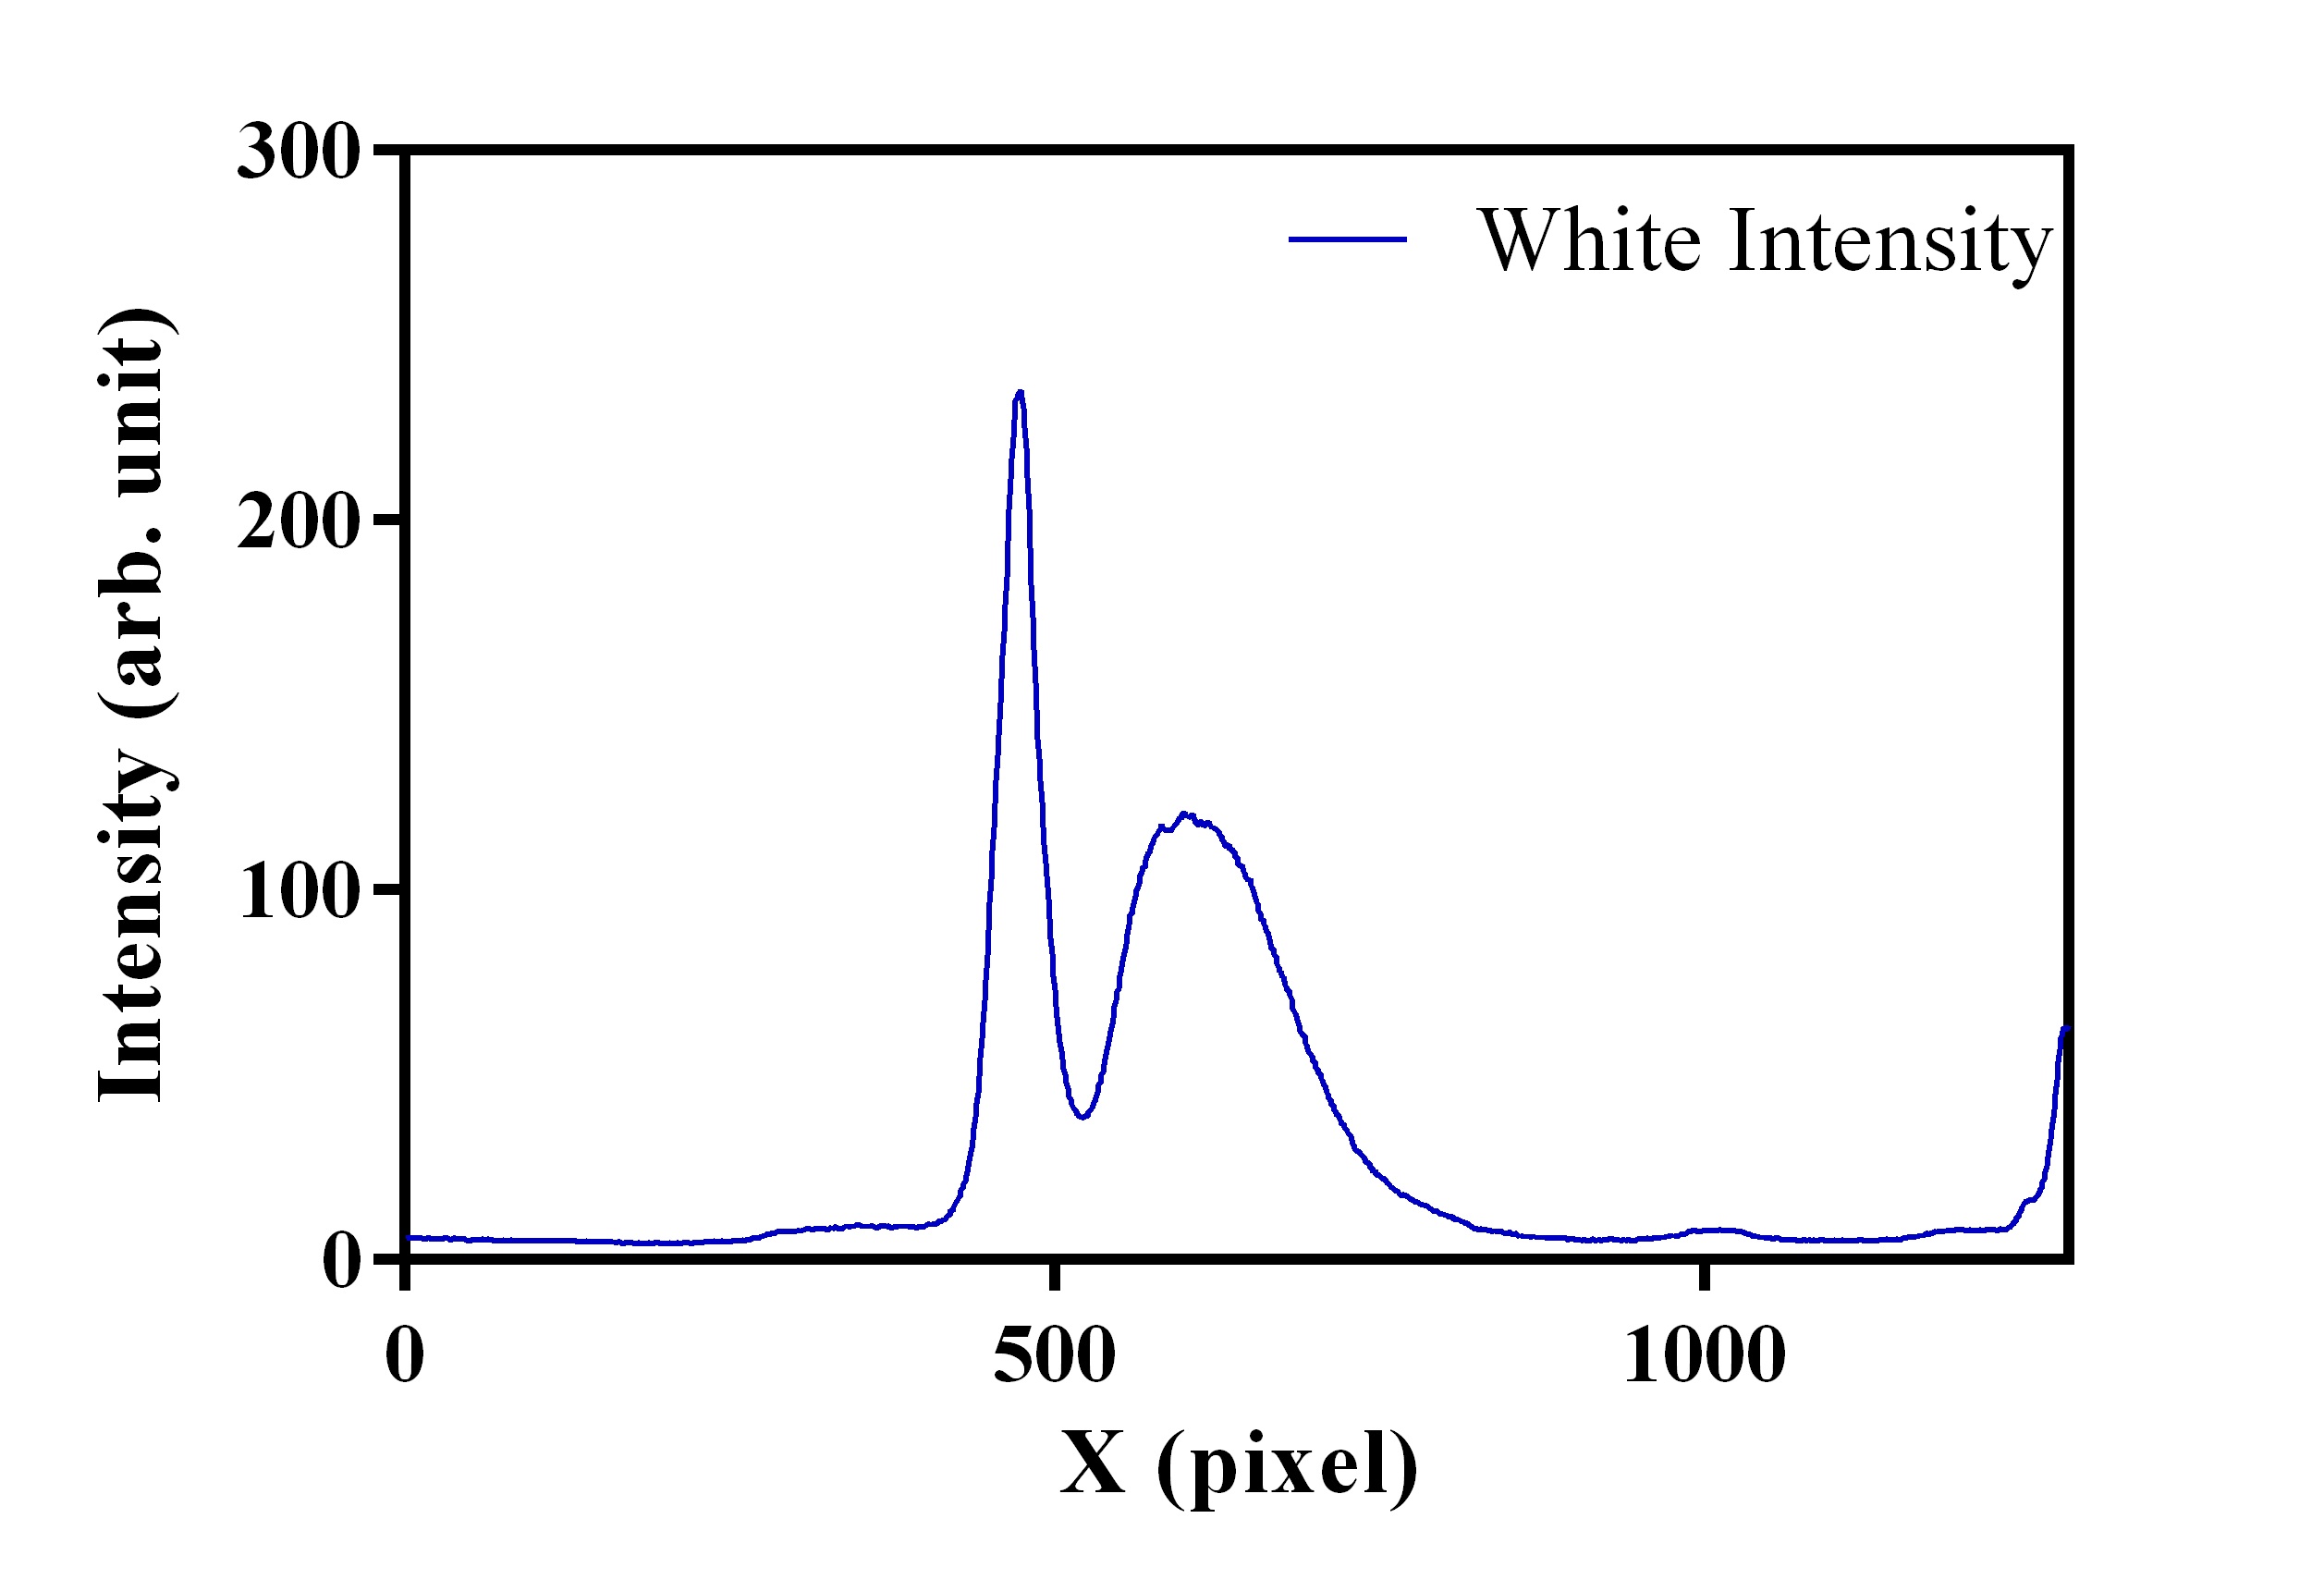
\includegraphics[width=\textwidth]{figures/White_As.PNG} %插入图片,[]中设置图片大小,{}中是图片文件名
	\caption{白光光譜經Auto Scaling後光譜波形表現} %最终文档中希望显示的图片标题
	\label{白光光譜經Auto Scaling後光譜波形表現} %用于文内引用的标签
\end{figure}
\par
但並非所有Auto Scaling都能將光譜調整至指定強度,如同表\ref{峰值位置比較表}. 所示,DG範圍受限在32\textasciitilde255之間,當一輸入光源過低而導致由公式(\ref{eq:2.6})所計算出的$DG_{goal}$超出255,則表示在Gamma = 100、BL = 0的條件下無法達成,因此需要調整其餘兩項參數,而又因Gamma與電雜訊將成正比升高,因此優先考慮調整BL,將BL由0至3階逐步升高,直至計算出的$DG_{goal}$小於255,若BL以達最高值仍然無法使$DG_{goal}$小於255,則將Gamma以每次增加50為一單位逐步提升,直至計算出的$DG_{goal}$小於255,若依然無法達成,僅剩更換較強光源這一選擇。\par
反之,當光源強度過強而導致由公式(\ref{eq:2.6})所計算出的$DG_{goal}$低於32時,由於此時$DG_{goal}$是以Gamma = 100、BL = 0的條件下所計算出,因此所有可調參數皆以達最低值,此時僅剩更換較低光源此一選項。所有Auto Scaling完整流程如圖\ref{Auto Scaling流程圖}. 所示。
\newpage
\begin{figure}[H] %H为当前位置,!htb为忽略美学标准,htbp为浮动图形
	\centering %图片居中
	\setlength{\abovecaptionskip}{1cm}
	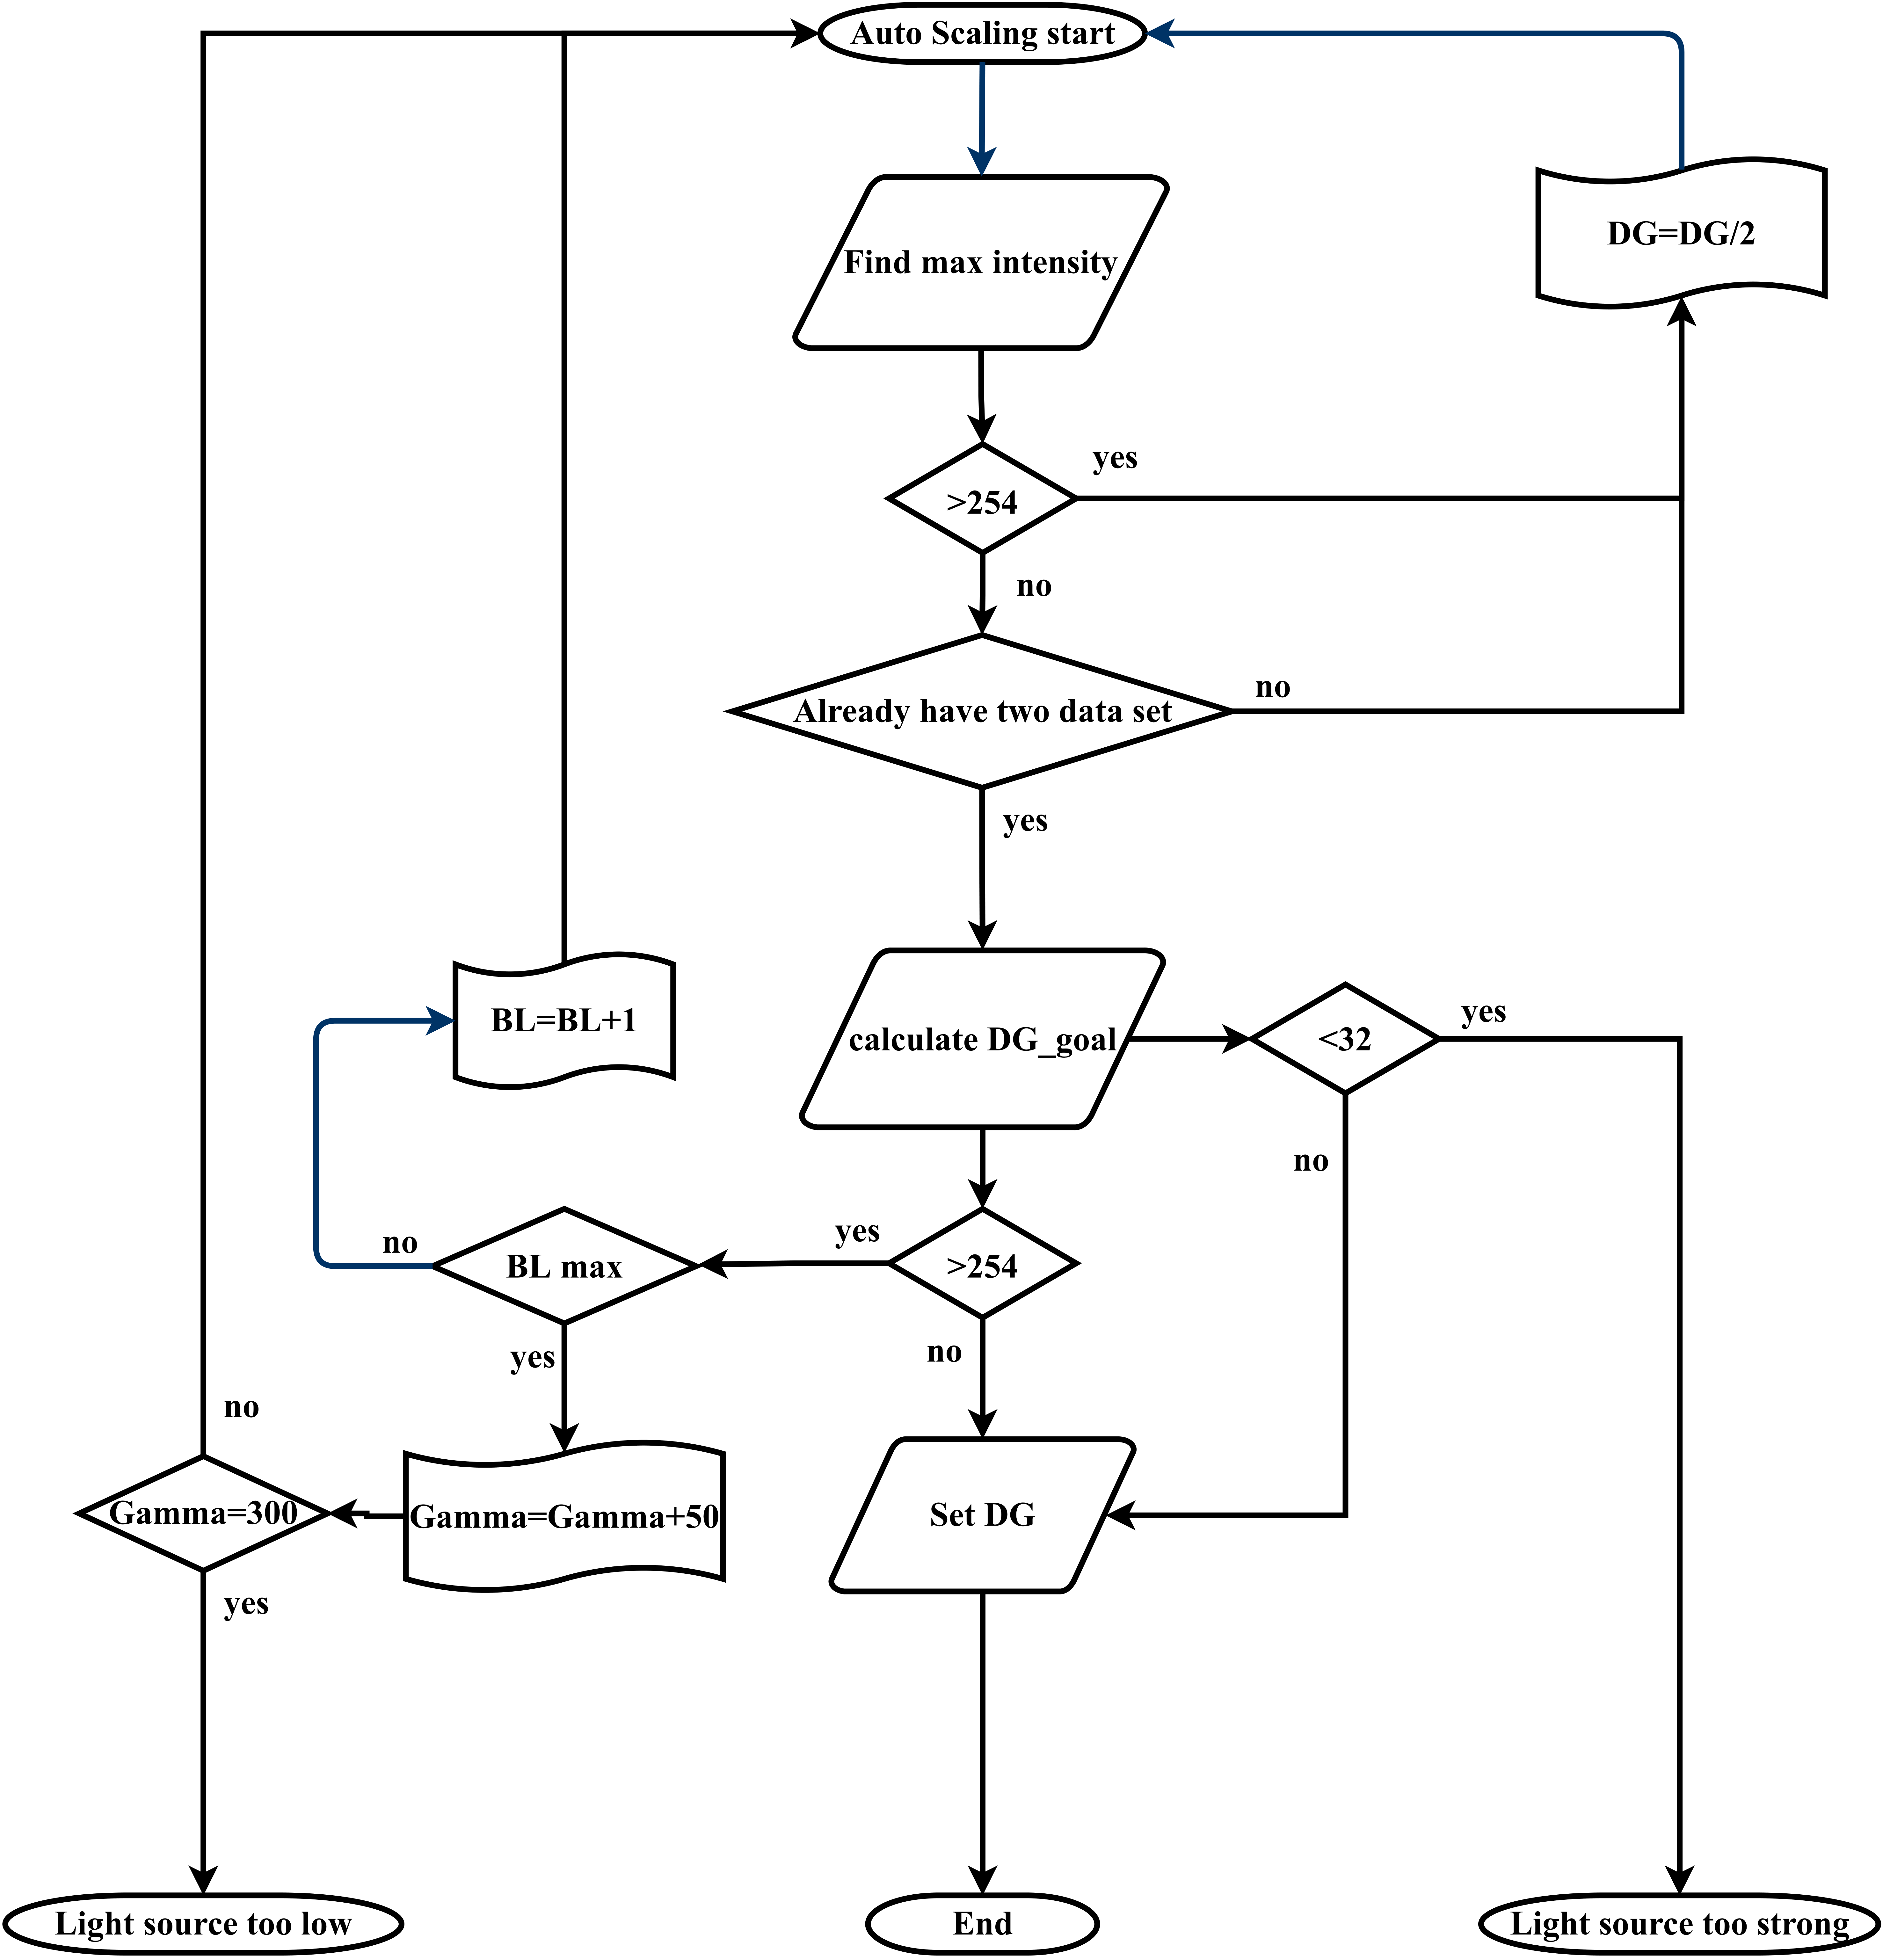
\includegraphics[width=\textwidth]{figures/Auto Scaling流程.png} %插入图片,[]中设置图片大小,{}中是图片文件名
	\caption{Auto Scaling流程圖} %最终文档中希望显示的图片标题
	\label{Auto Scaling流程圖} %用于文内引用的标签
\end{figure}

\newpage
\section{波峰位置偵測}
Auto Scaling後的光譜波形十分適合分析,由於不存在任何過曝點,故擬合後找出的峰值較為精確。本文欲結合使用雷射光與汞氬燈的波峰位置的像素與其標準參考波長做為波長校正之擬合點,因此需個別找出兩種光源的參考波峰,並經由勞倫茲擬和找出精確波峰位置,並存於記憶體之中,直至所有波峰位置皆被找出,便可以將所有波峰的像素位置與標準波長一起進行多項式擬合。\par
完整波峰查詢的標準流程如圖\ref{波峰位置偵測流程圖}. ,,但又因汞燈與氬燈強度差異過大,加上不同晶片於不同波段效率不同,礙於這兩點演算法上難以解決的困難,因此汞氬燈光譜進行波峰位置偵測前,將對數據進行汞燈與氬燈的分離,並在不同的影像感測器參數下,分別取出光譜後再進行波峰位置偵測,詳細流程本文於3.5.1節說明。
\begin{figure}[H] %H为当前位置,!htb为忽略美学标准,htbp为浮动图形
	\centering %图片居中
	\vspace{0.8cm}
	\setlength{\abovecaptionskip}{0.8cm}
	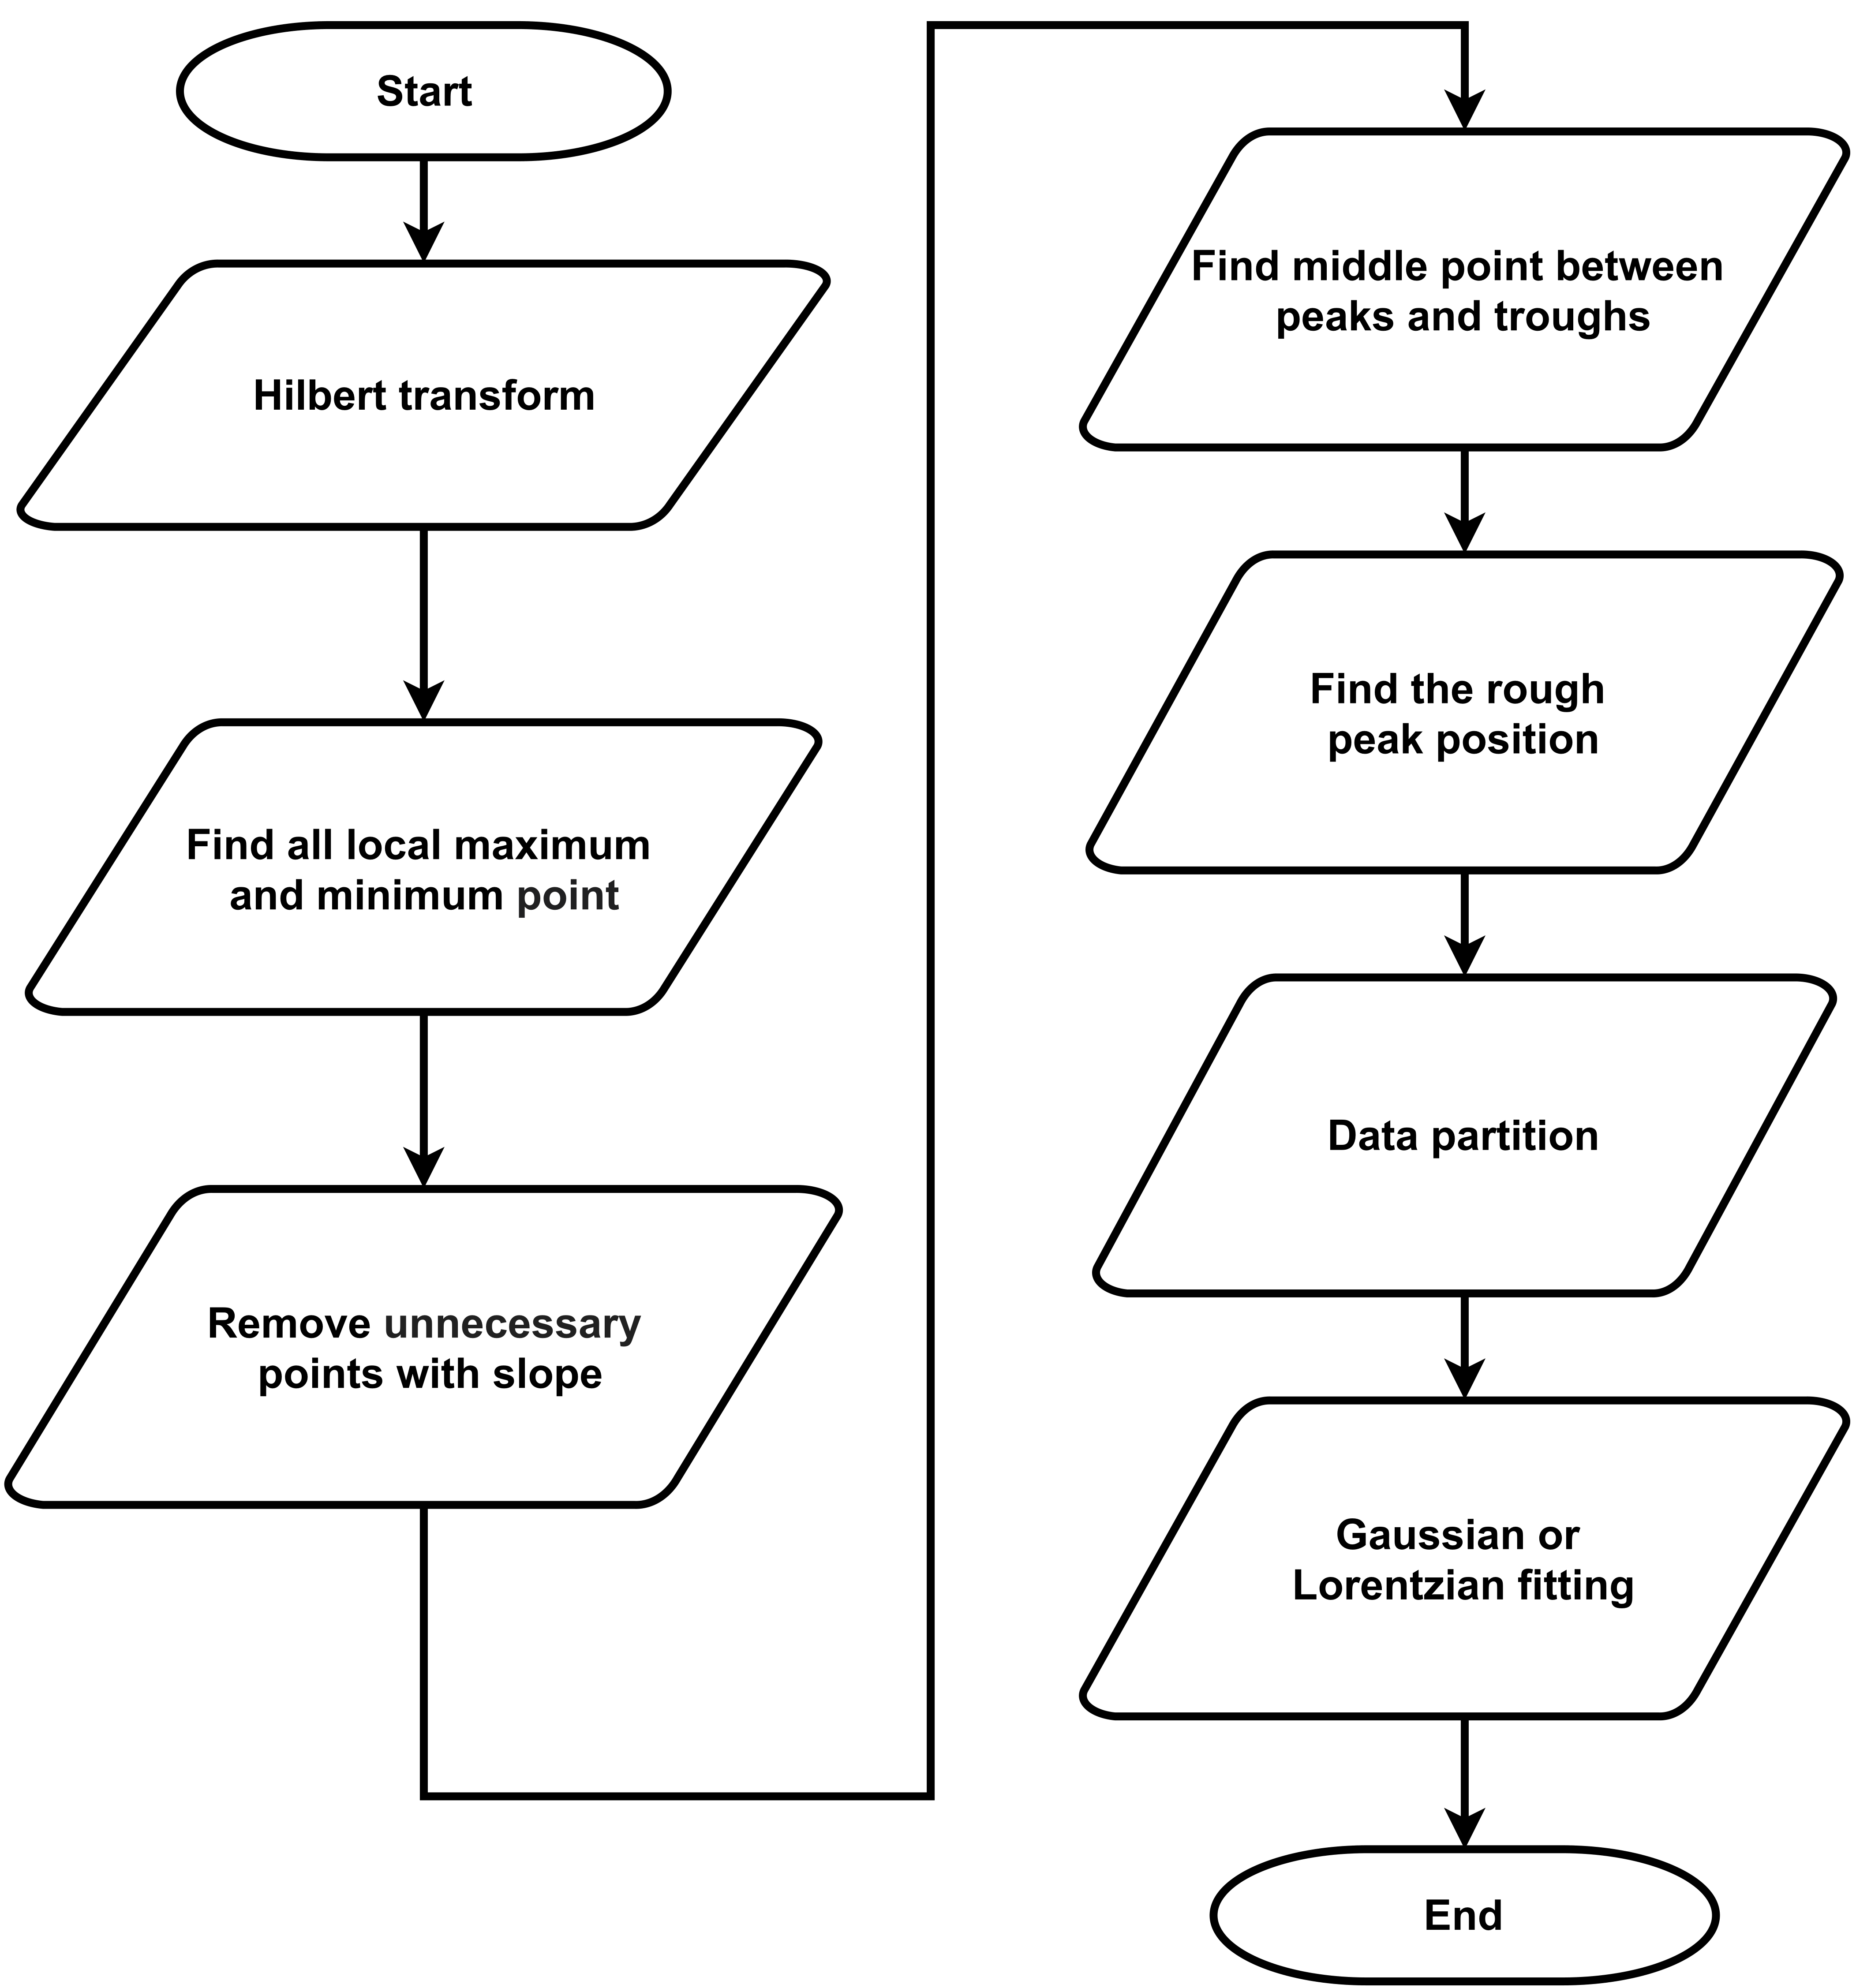
\includegraphics[width=0.7\textwidth]{figures/FINDPEAK_FLOWCHART.png} %插入图片,[]中设置图片大小,{}中是图片文件名
	\caption{波峰位置偵測流程圖} %最终文档中希望显示的图片标题
	\label{波峰位置偵測流程圖} %用于文内引用的标签
\end{figure}

\subsection{汞氬燈波峰位置偵測}
當一汞氬燈的ROI影像經過Auto Scaling後的光譜如圖\ref{Auto Scaling後汞氬燈光譜圖}. 所示,汞氬燈中的汞燈與氬燈為同時激發產生之光束,因此無法將兩數據分離,而汞燈強度與氬燈強度明顯相差極大,造成演算法難以在不同效率的晶片下穩定找到每一個波峰,所以汞燈與氬燈並非所有波峰皆適合用於波長校正,必需挑選符合要求並穩定的波峰。
\par 
適合做為波長校正波峰的條件為特徵明顯且峰與峰之間不宜距離過近,距離過近的峰值對於擬和的貢獻並不大,因此本文挑選適合做為波長校正參考波峰的汞燈與氬燈波峰的標準波長位置如表\ref{汞氬燈標準波峰位置表}. 所示。
\begin{figure}[H] %H为当前位置,!htb为忽略美学标准,htbp为浮动图形
	\centering %图片居中
	\vspace{0.8cm}
	\setlength{\abovecaptionskip}{0.cm}
	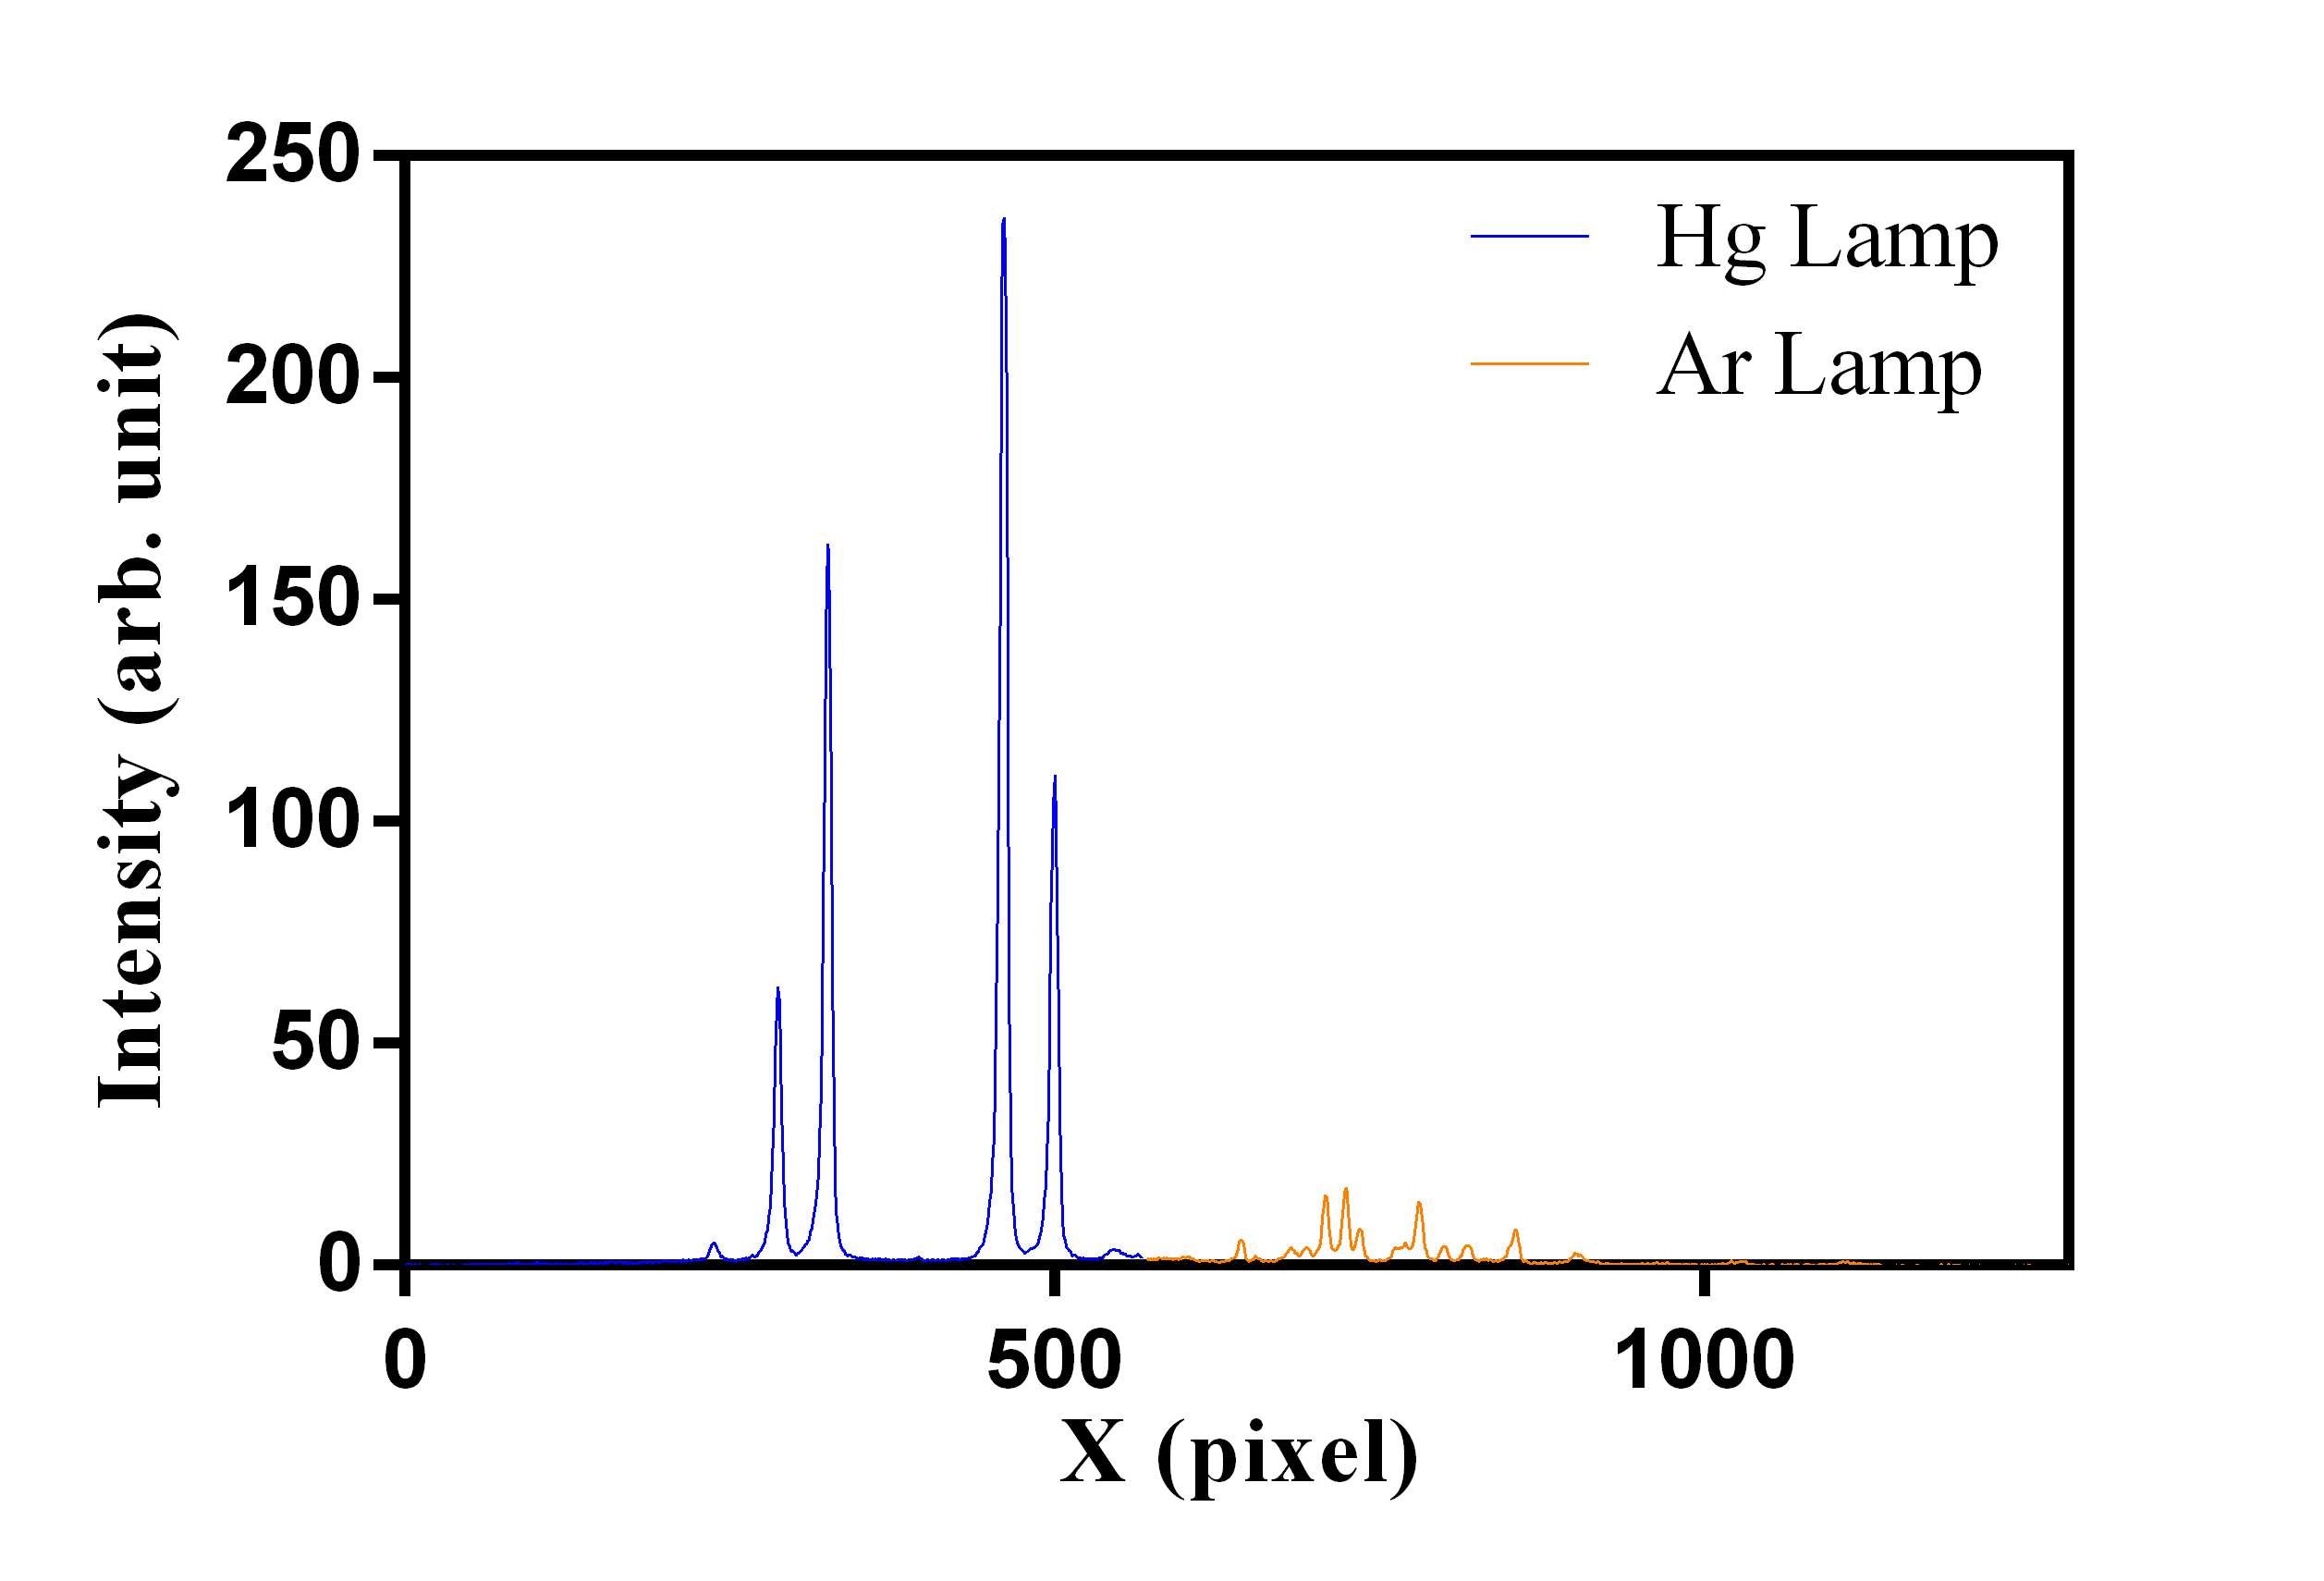
\includegraphics[width=\textwidth]{figures/HG_AR_LAMP.PNG} %插入图片,[]中设置图片大小,{}中是图片文件名
	\caption{Auto Scaling後汞氬燈光譜圖} %最终文档中希望显示的图片标题
	\label{Auto Scaling後汞氬燈光譜圖} %用于文内引用的标签
\end{figure}
\newpage
\begin{center}
\vspace{0.8cm}
\captionof{table}{汞氬燈標準波峰位置表}\label{汞氬燈標準波峰位置表}
\begin{tabularx}{\textwidth}{m{0.33\textwidth}<{\centering} m{0.25\textwidth}<{\centering} m{0.33\textwidth}<{\centering}}
	\hline\hline
          & 汞燈 & 氬燈 \\
	\hline
	\multirow{4}{*}{標準波峰位置(nm) }
	      & 404.65 & 763.51 \\
	      & 435.83 & 811.53 \\
	      & 546.07 & -- \\
	      & 578.01 & -- \\
	\hline\hline
\end{tabularx}
\vspace{10pt}
\end{center}
\par
表\ref{汞氬燈標準波峰位置表}. 中的六個波峰,橫跨短波長至長波長波段,對於每個波段皆有擬合貢獻,因此相當適合做為波長校正的擬和點,且強度較其餘波峰強的許多,利於波峰偵測,故此六個波峰為汞氬燈波峰偵測的目標波峰,而這些波峰位置在圖\ref{汞氬燈目標波峰位置圖}. 標示於波長空間中。
\begin{figure}[H] %H为当前位置,!htb为忽略美学标准,htbp为浮动图形
	\centering %图片居中
	\vspace{0.8cm} 
	\setlength{\abovecaptionskip}{0.cm}
	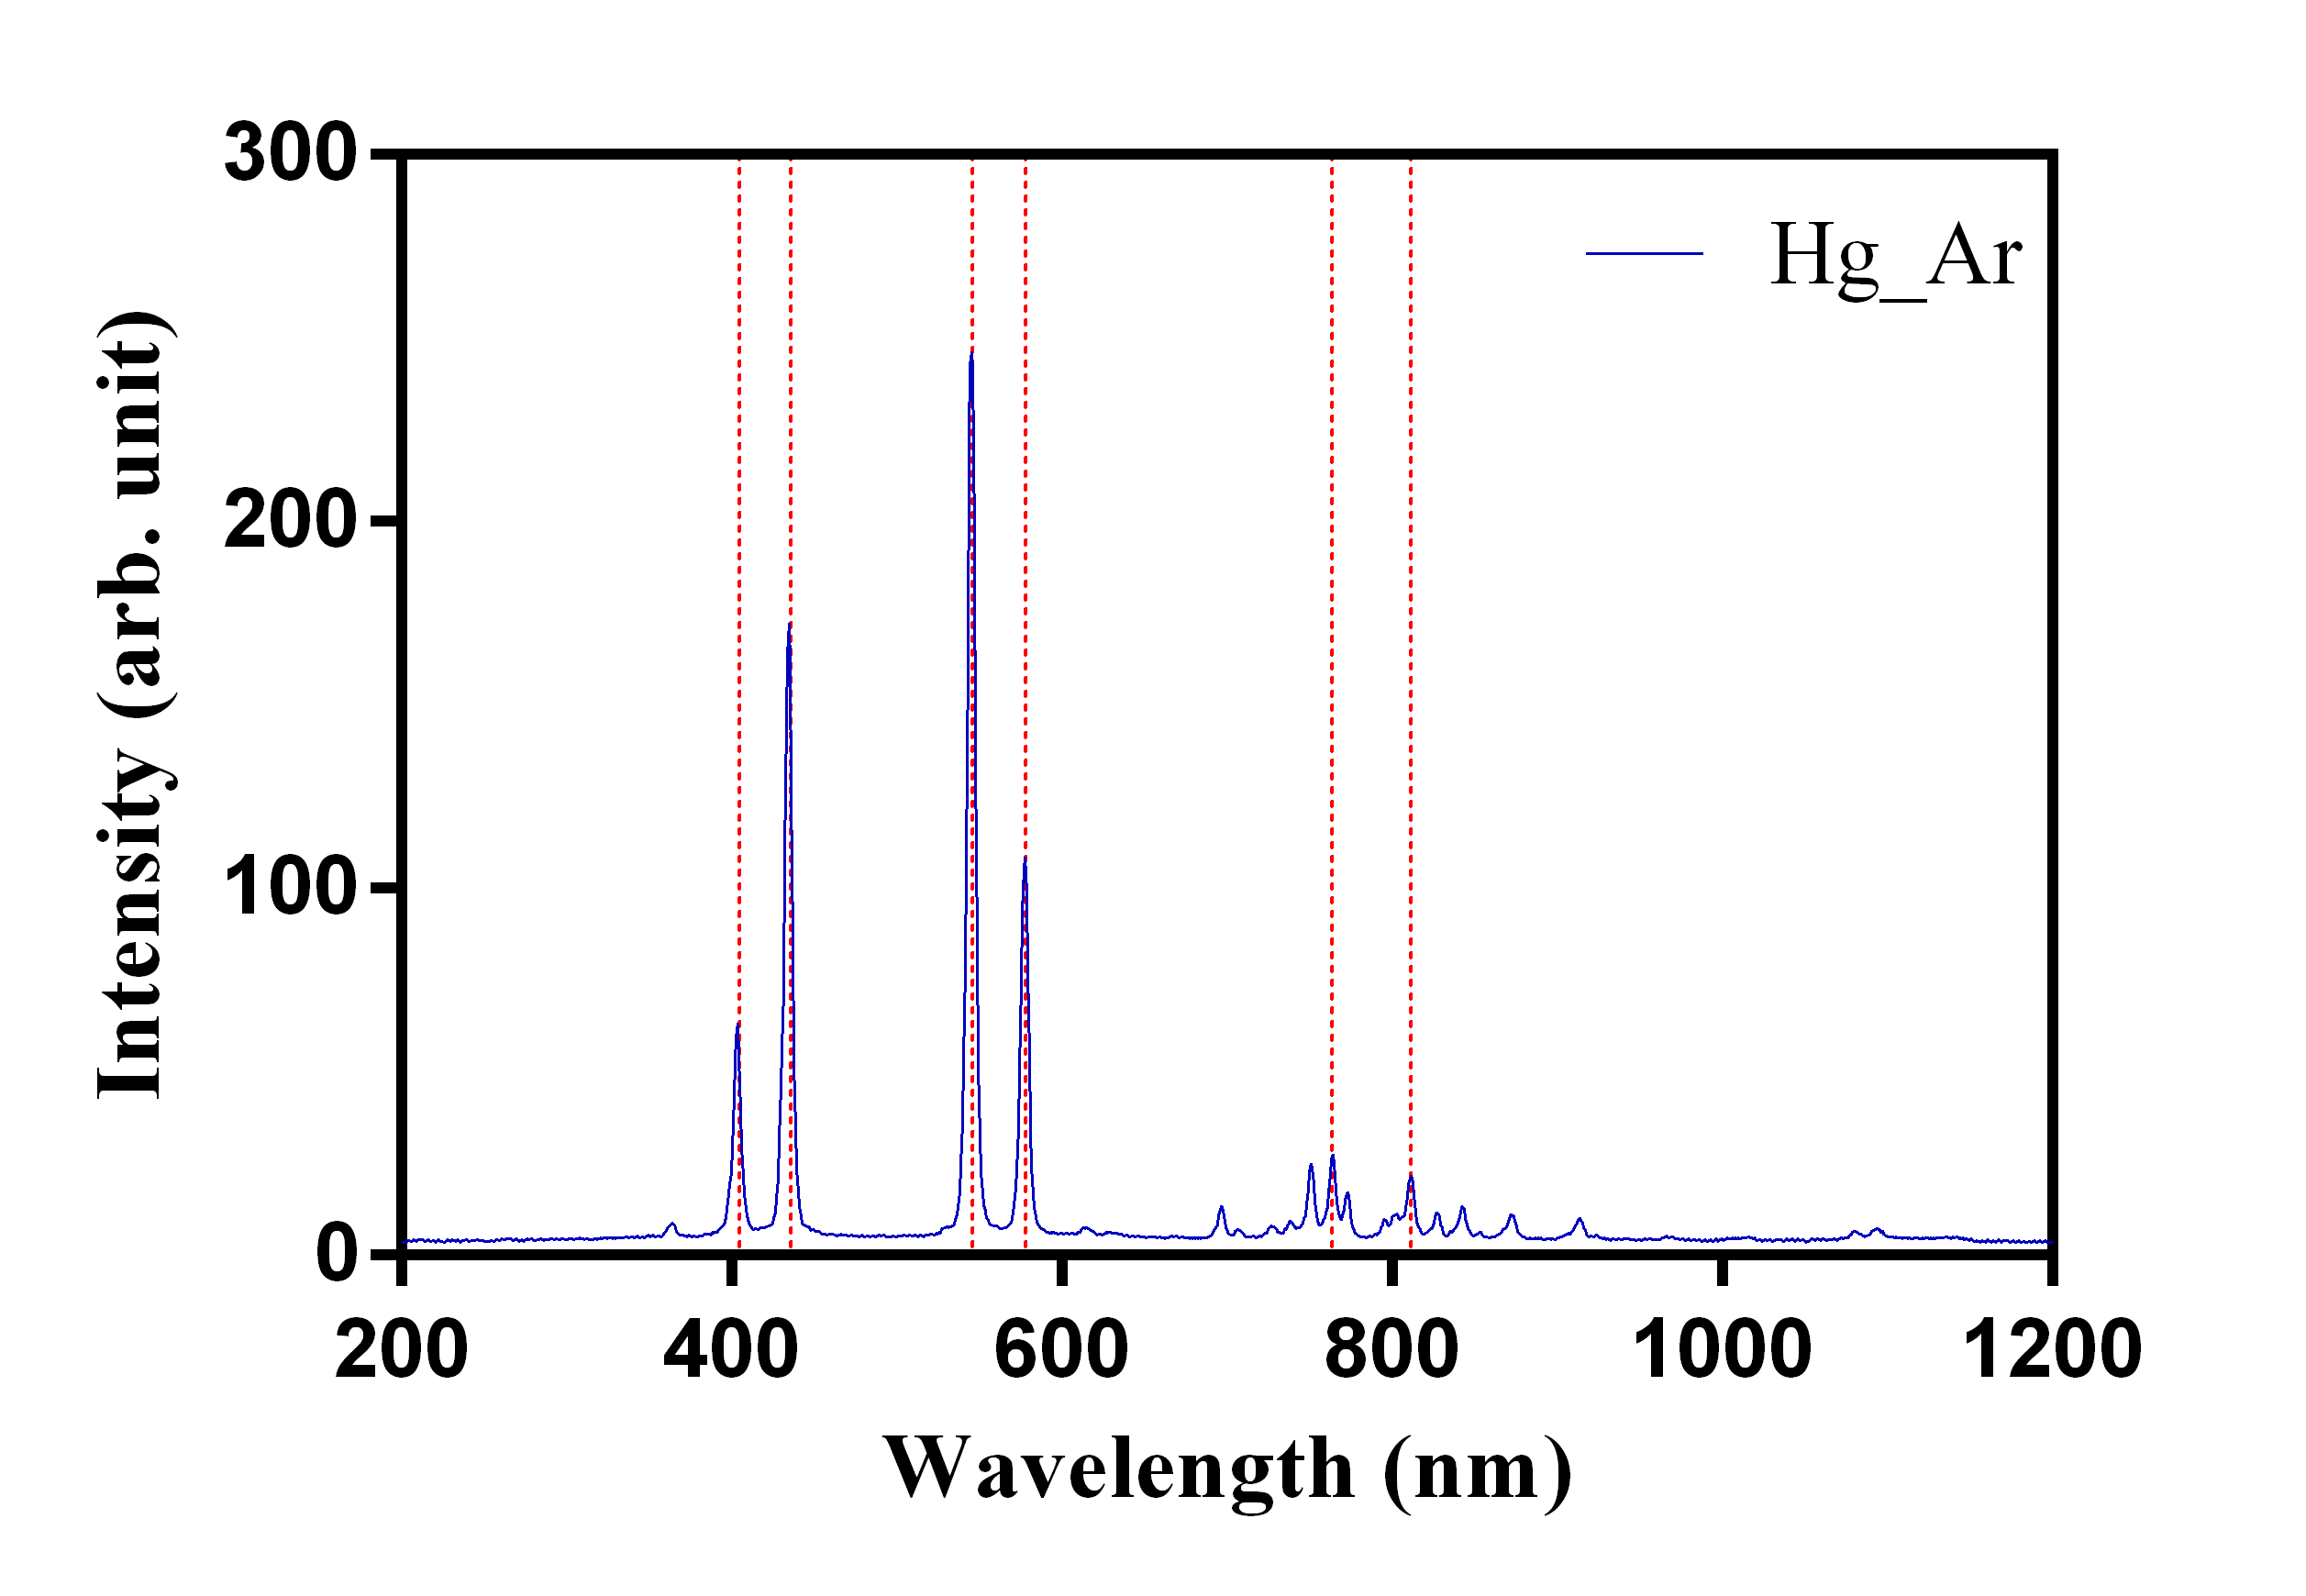
\includegraphics[width=\textwidth]{figures/HgAr_Wavelength.png} %插入图片,[]中设置图片大小,{}中是图片文件名
	\caption{汞氬燈目標波峰位置圖} %最终文档中希望显示的图片标题
	\label{汞氬燈目標波峰位置圖} %用于文内引用的标签
\end{figure}
\newpage

由於目標波峰涵蓋汞燈波峰與氬燈波峰,又因氬燈與汞燈強度落差極為巨大,造成波峰偵測時的強度閥值與斜率閥值難以界定,因不同晶片效能不同,光譜強度難以重現,若以原始數據及固定閥值界定是否為有效波峰,將會出現氬燈在效率較低之晶片時波峰無法被完全偵測,反之則在效率高的晶片時發生雜訊被判定為波峰。\par
光譜雖在像素空間會因影像感測器的因素而有平移,強度也會有所不同,造成每次量測時波峰落在不同的位置與不同的強度,但因任何物質的光譜波長位置與光譜趨勢是唯一且不變的,因此所有波峰的距離是固定的,所以不同空間中的光譜波型是不會改變的,波峰的距離也是固定的,本文利用此一光譜特性,透過數據中的最大值像素位置與像素距離界定出汞燈與氬燈的數據分界點,如圖\ref{汞氬燈數據分區交界點}. 所示。
\begin{figure}[H] %H为当前位置,!htb为忽略美学标准,htbp为浮动图形
	\centering %图片居中
	\vspace{0.8cm}
	\setlength{\abovecaptionskip}{0.cm}
	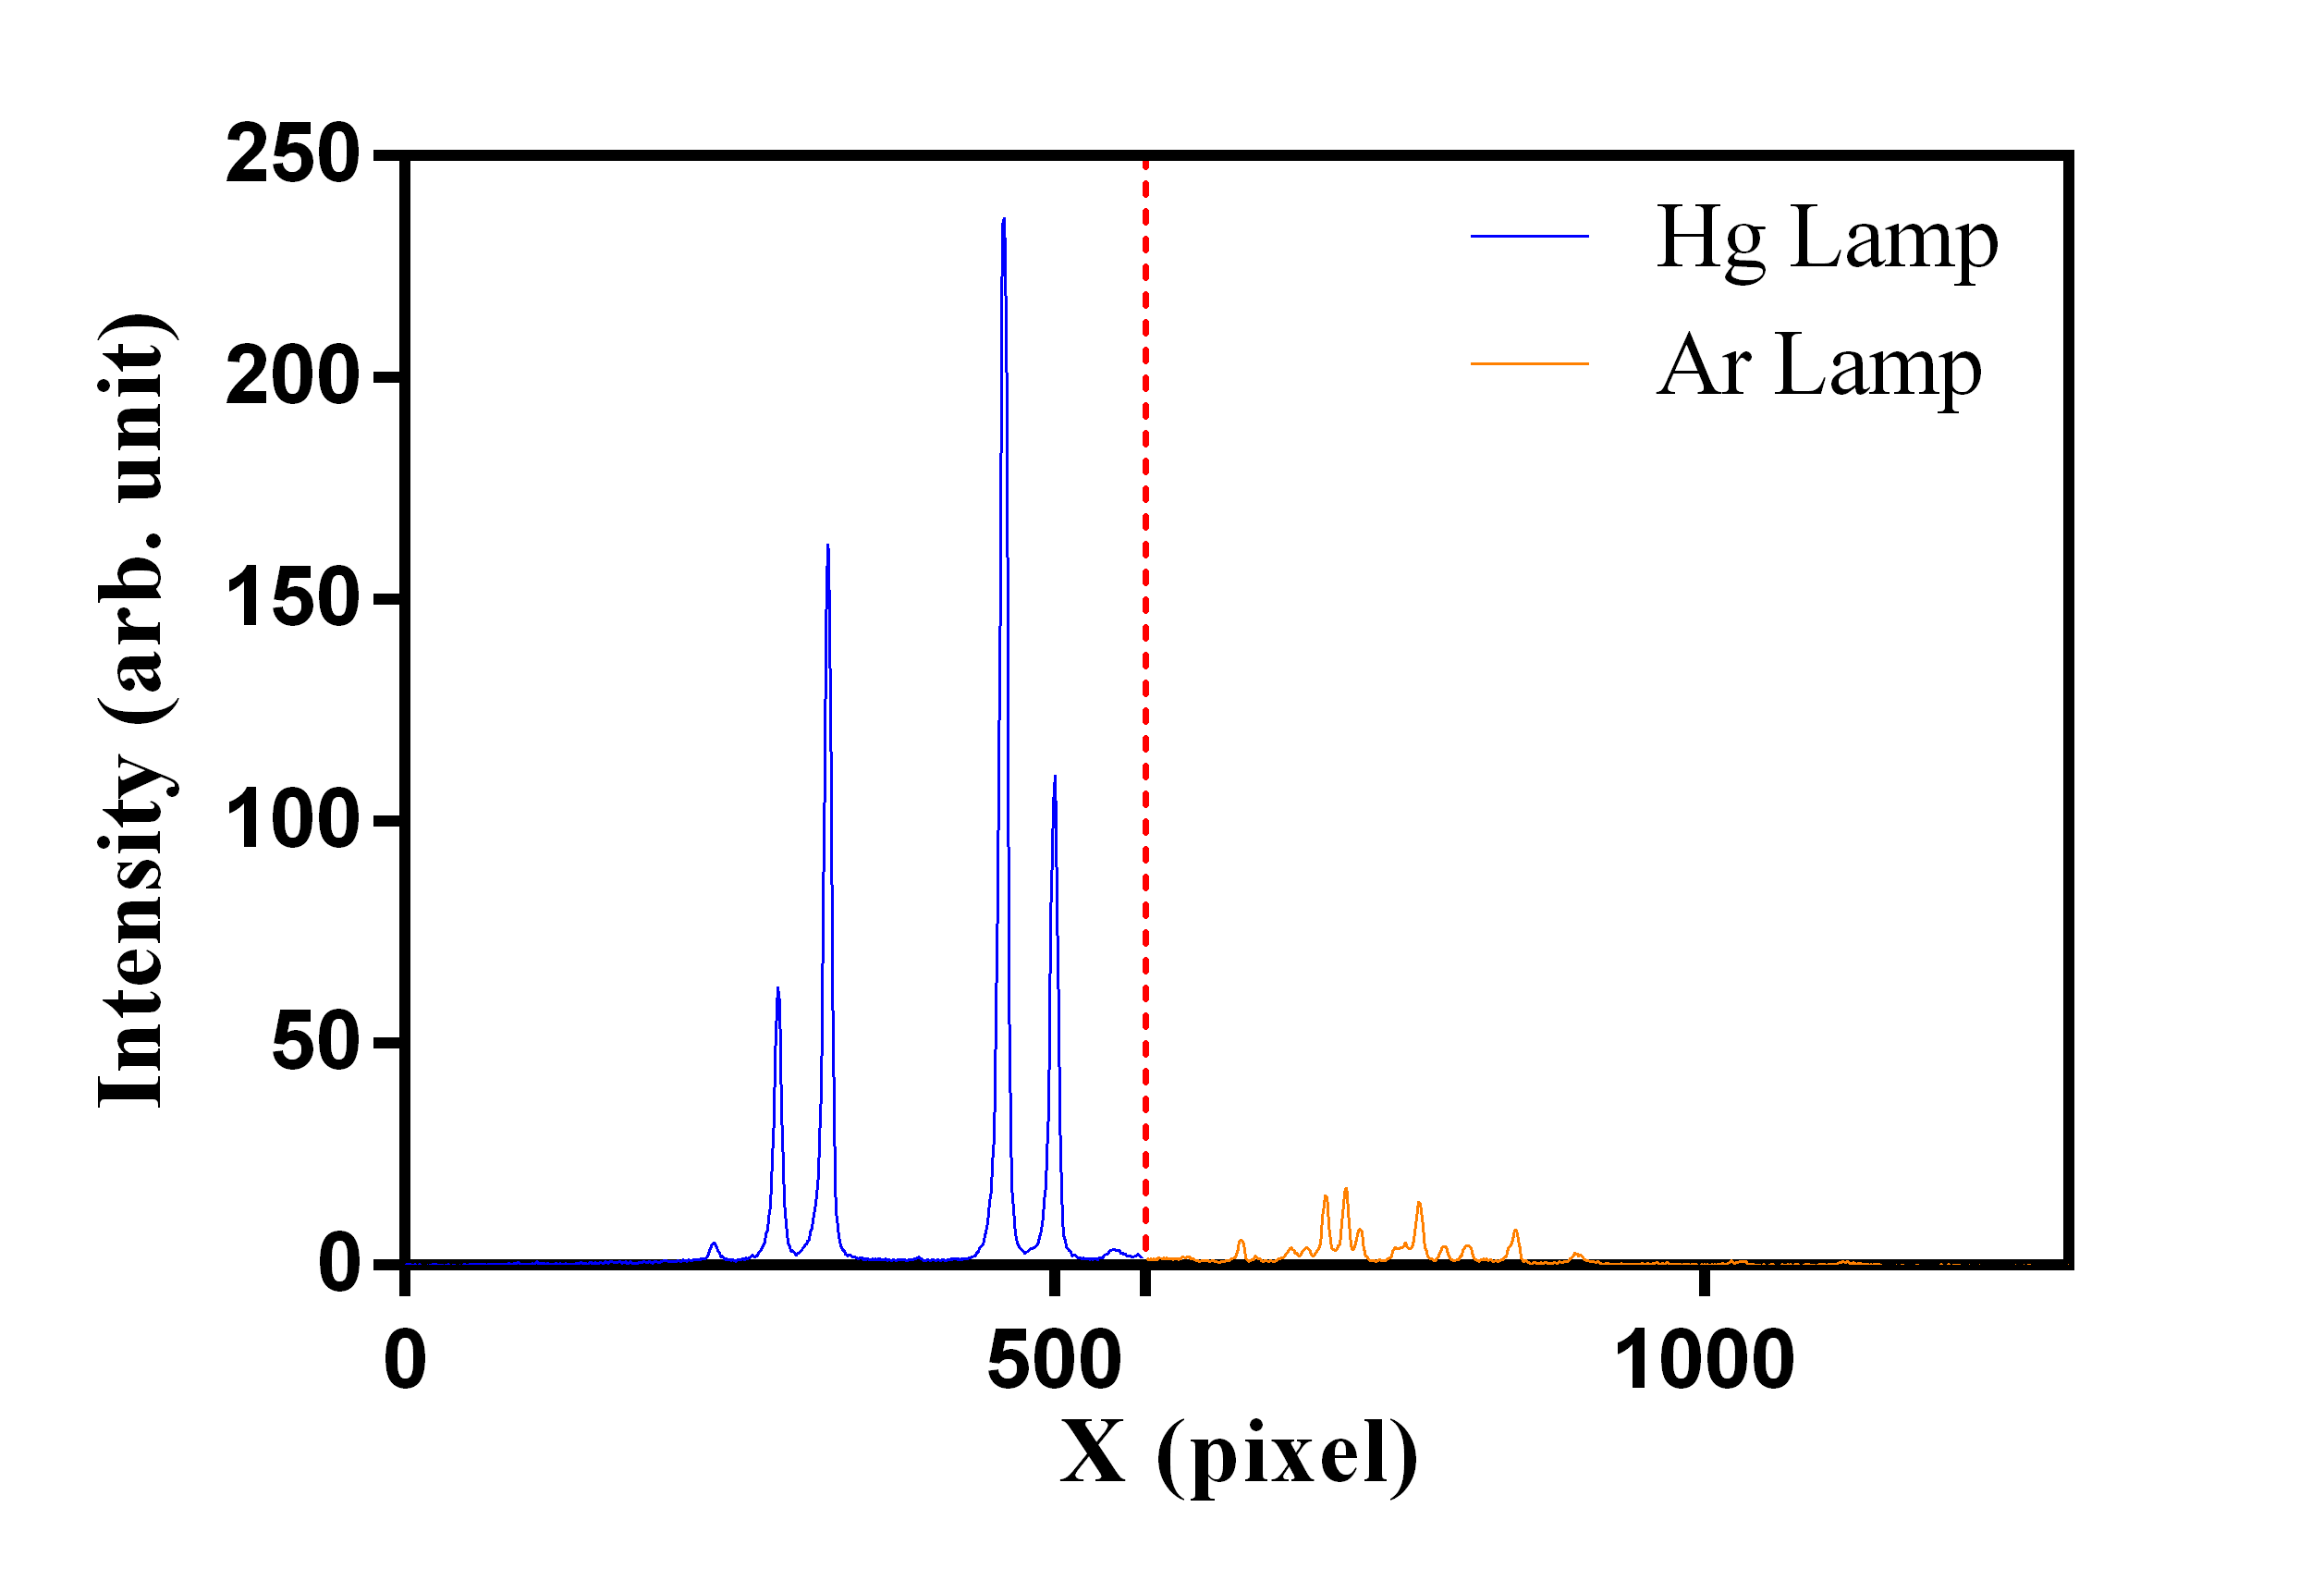
\includegraphics[width=\textwidth]{figures/JunctionPoint.png} %插入图片,[]中设置图片大小,{}中是图片文件名
	\caption{汞氬燈數據分區交界點} %最终文档中希望显示的图片标题
	\label{汞氬燈數據分區交界點} %用于文内引用的标签
\end{figure}
將汞燈氬燈數據個別區分後,由於此組原始數據已經進行過一次Auto Scaling,因此汞燈區域已完成強度調整,僅需對氬燈區域數據再進行一次Auto Scaling,使氬燈區域光譜強度達到適當值如圖\ref{氬燈數據AutoScaling後光譜波形圖}. 所示,再將兩組數據合併進行波峰偵測,即可達到平衡汞燈與氬燈間的強度落差,結合後光譜數據如圖\ref{氬燈數據AutoScaling並合併後光譜波形圖}. 所示。
\begin{figure}[H] %H为当前位置,!htb为忽略美学标准,htbp为浮动图形
	\centering %图片居中
	\vspace{0.8cm}
	\setlength{\abovecaptionskip}{0.cm}
	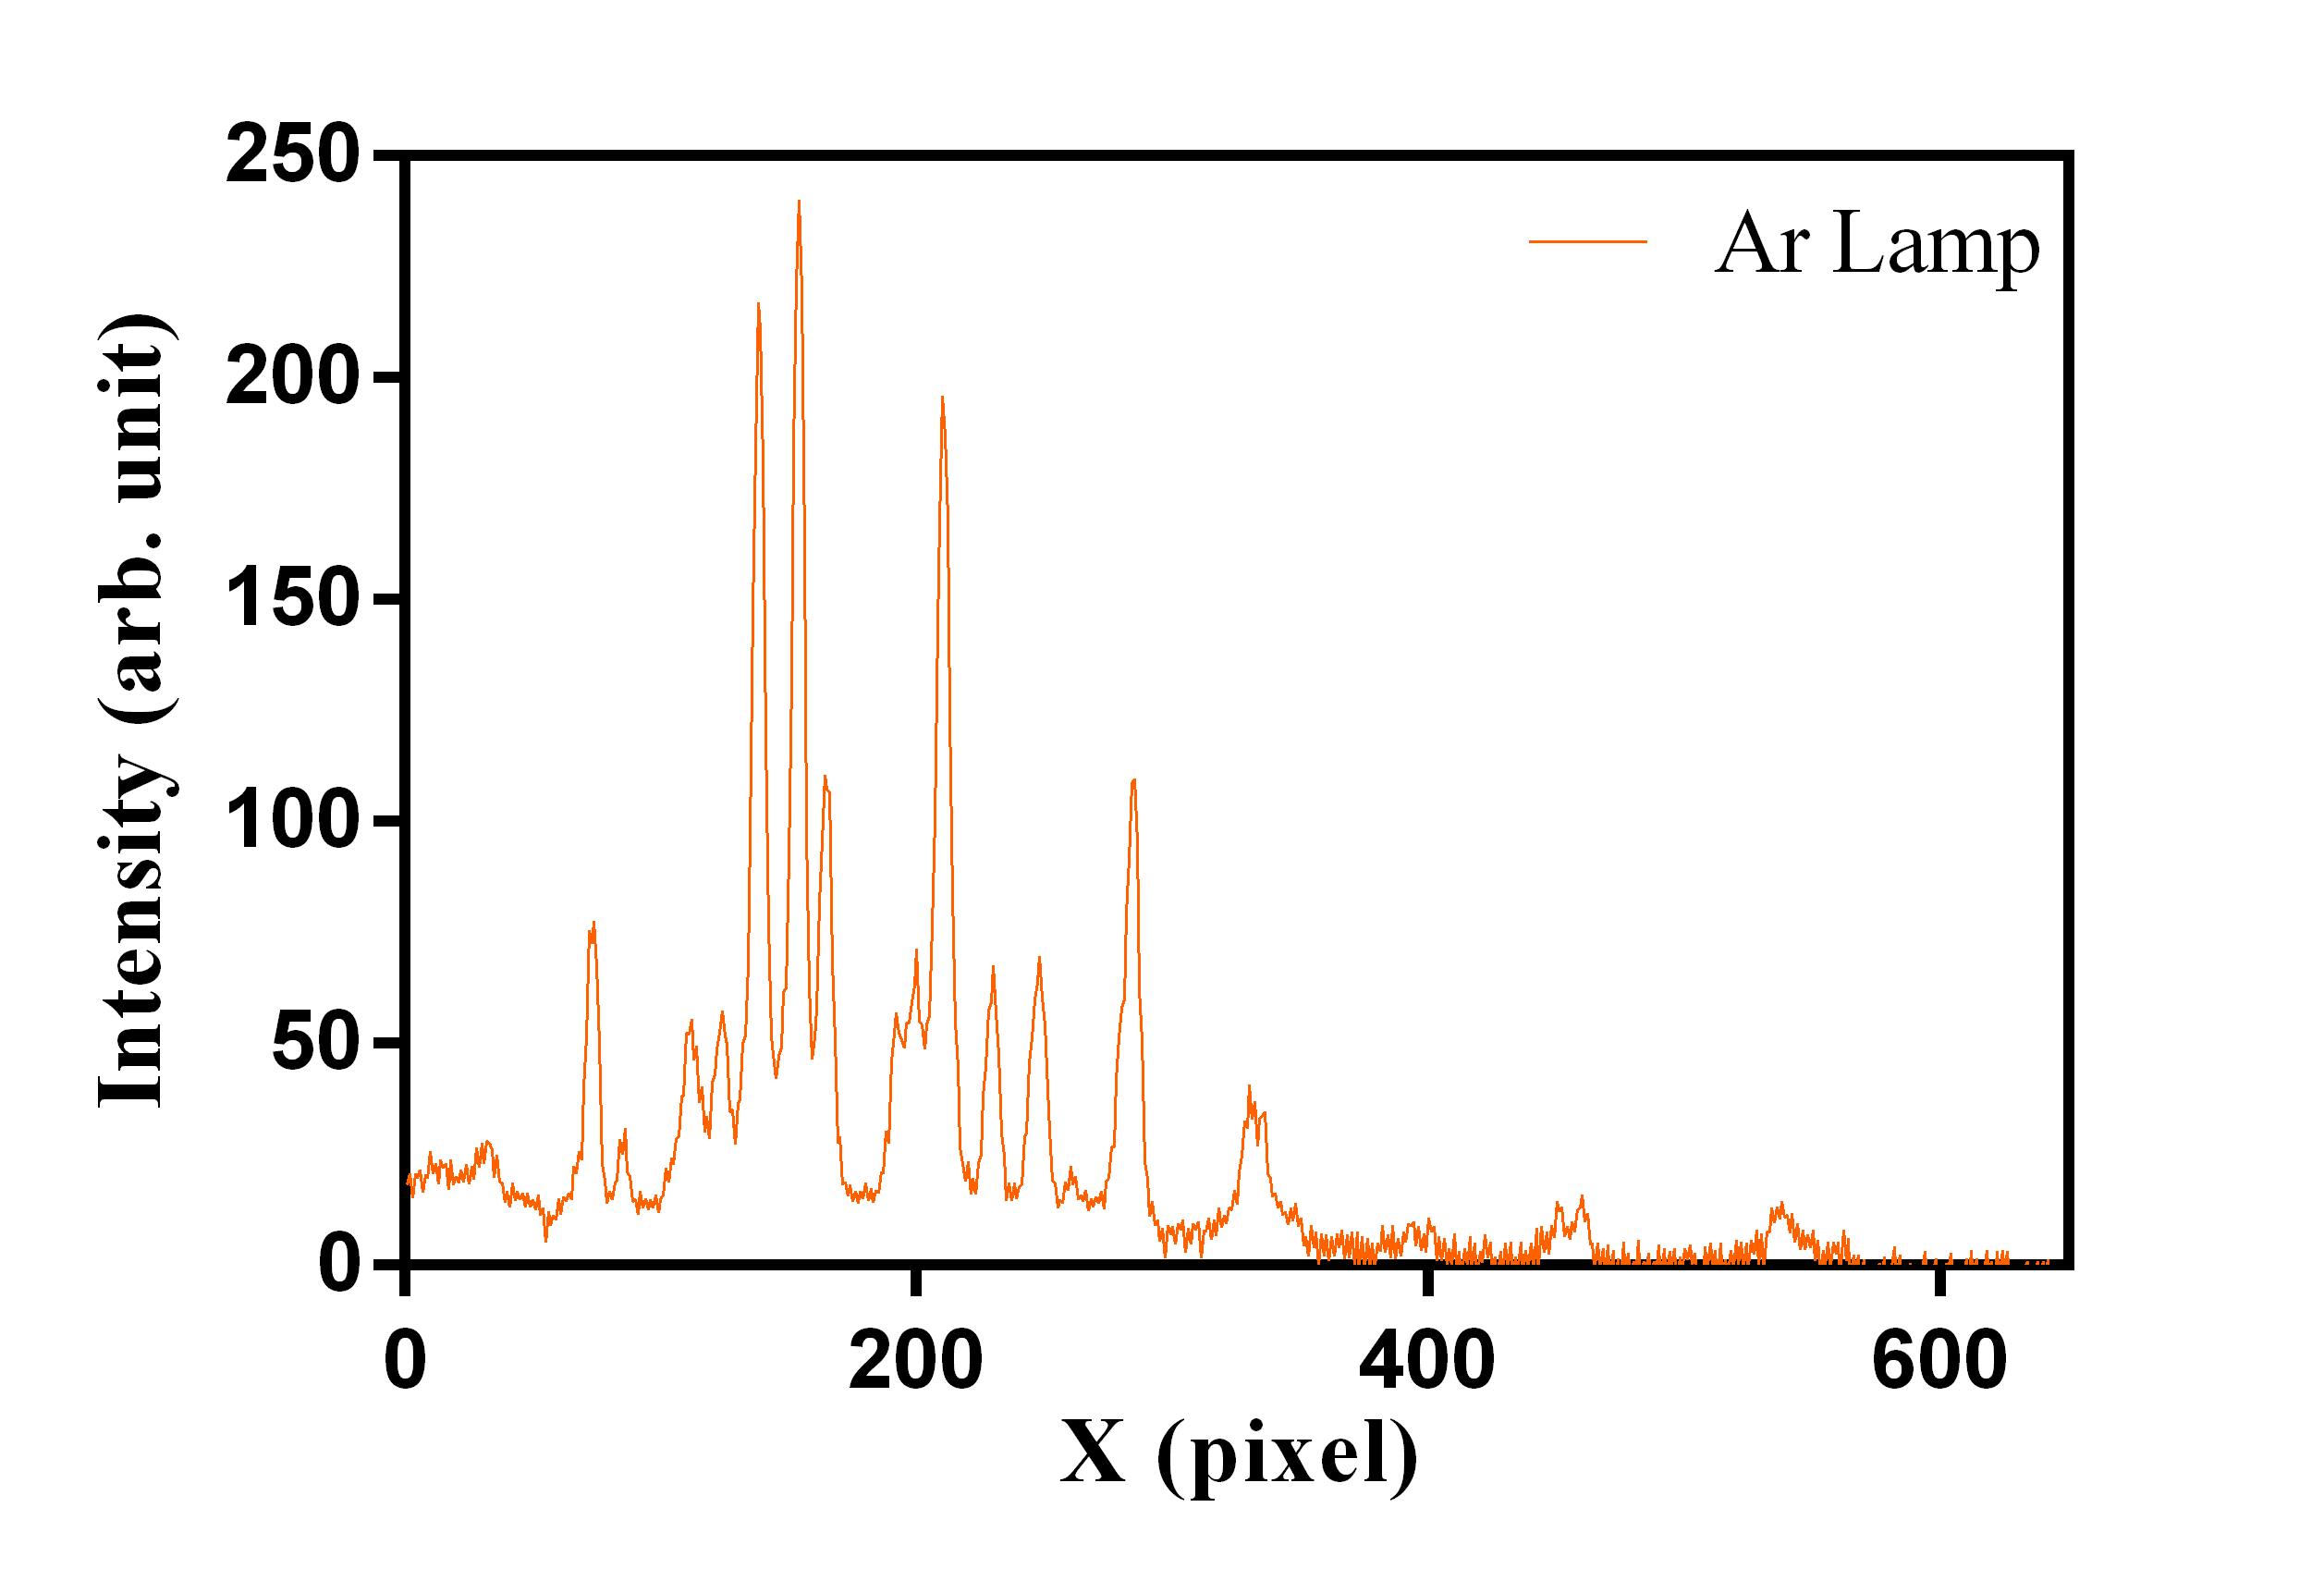
\includegraphics[width=15cm]{figures/ArLamp.png} %插入图片,[]中设置图片大小,{}中是图片文件名
	\caption{氬燈數據AutoScaling後光譜波形圖} %最终文档中希望显示的图片标题
	\label{氬燈數據AutoScaling後光譜波形圖} %用于文内引用的标签
\end{figure}

\begin{figure}[H] %H为当前位置,!htb为忽略美学标准,htbp为浮动图形
	\centering %图片居中
	\setlength{\abovecaptionskip}{0.cm}
	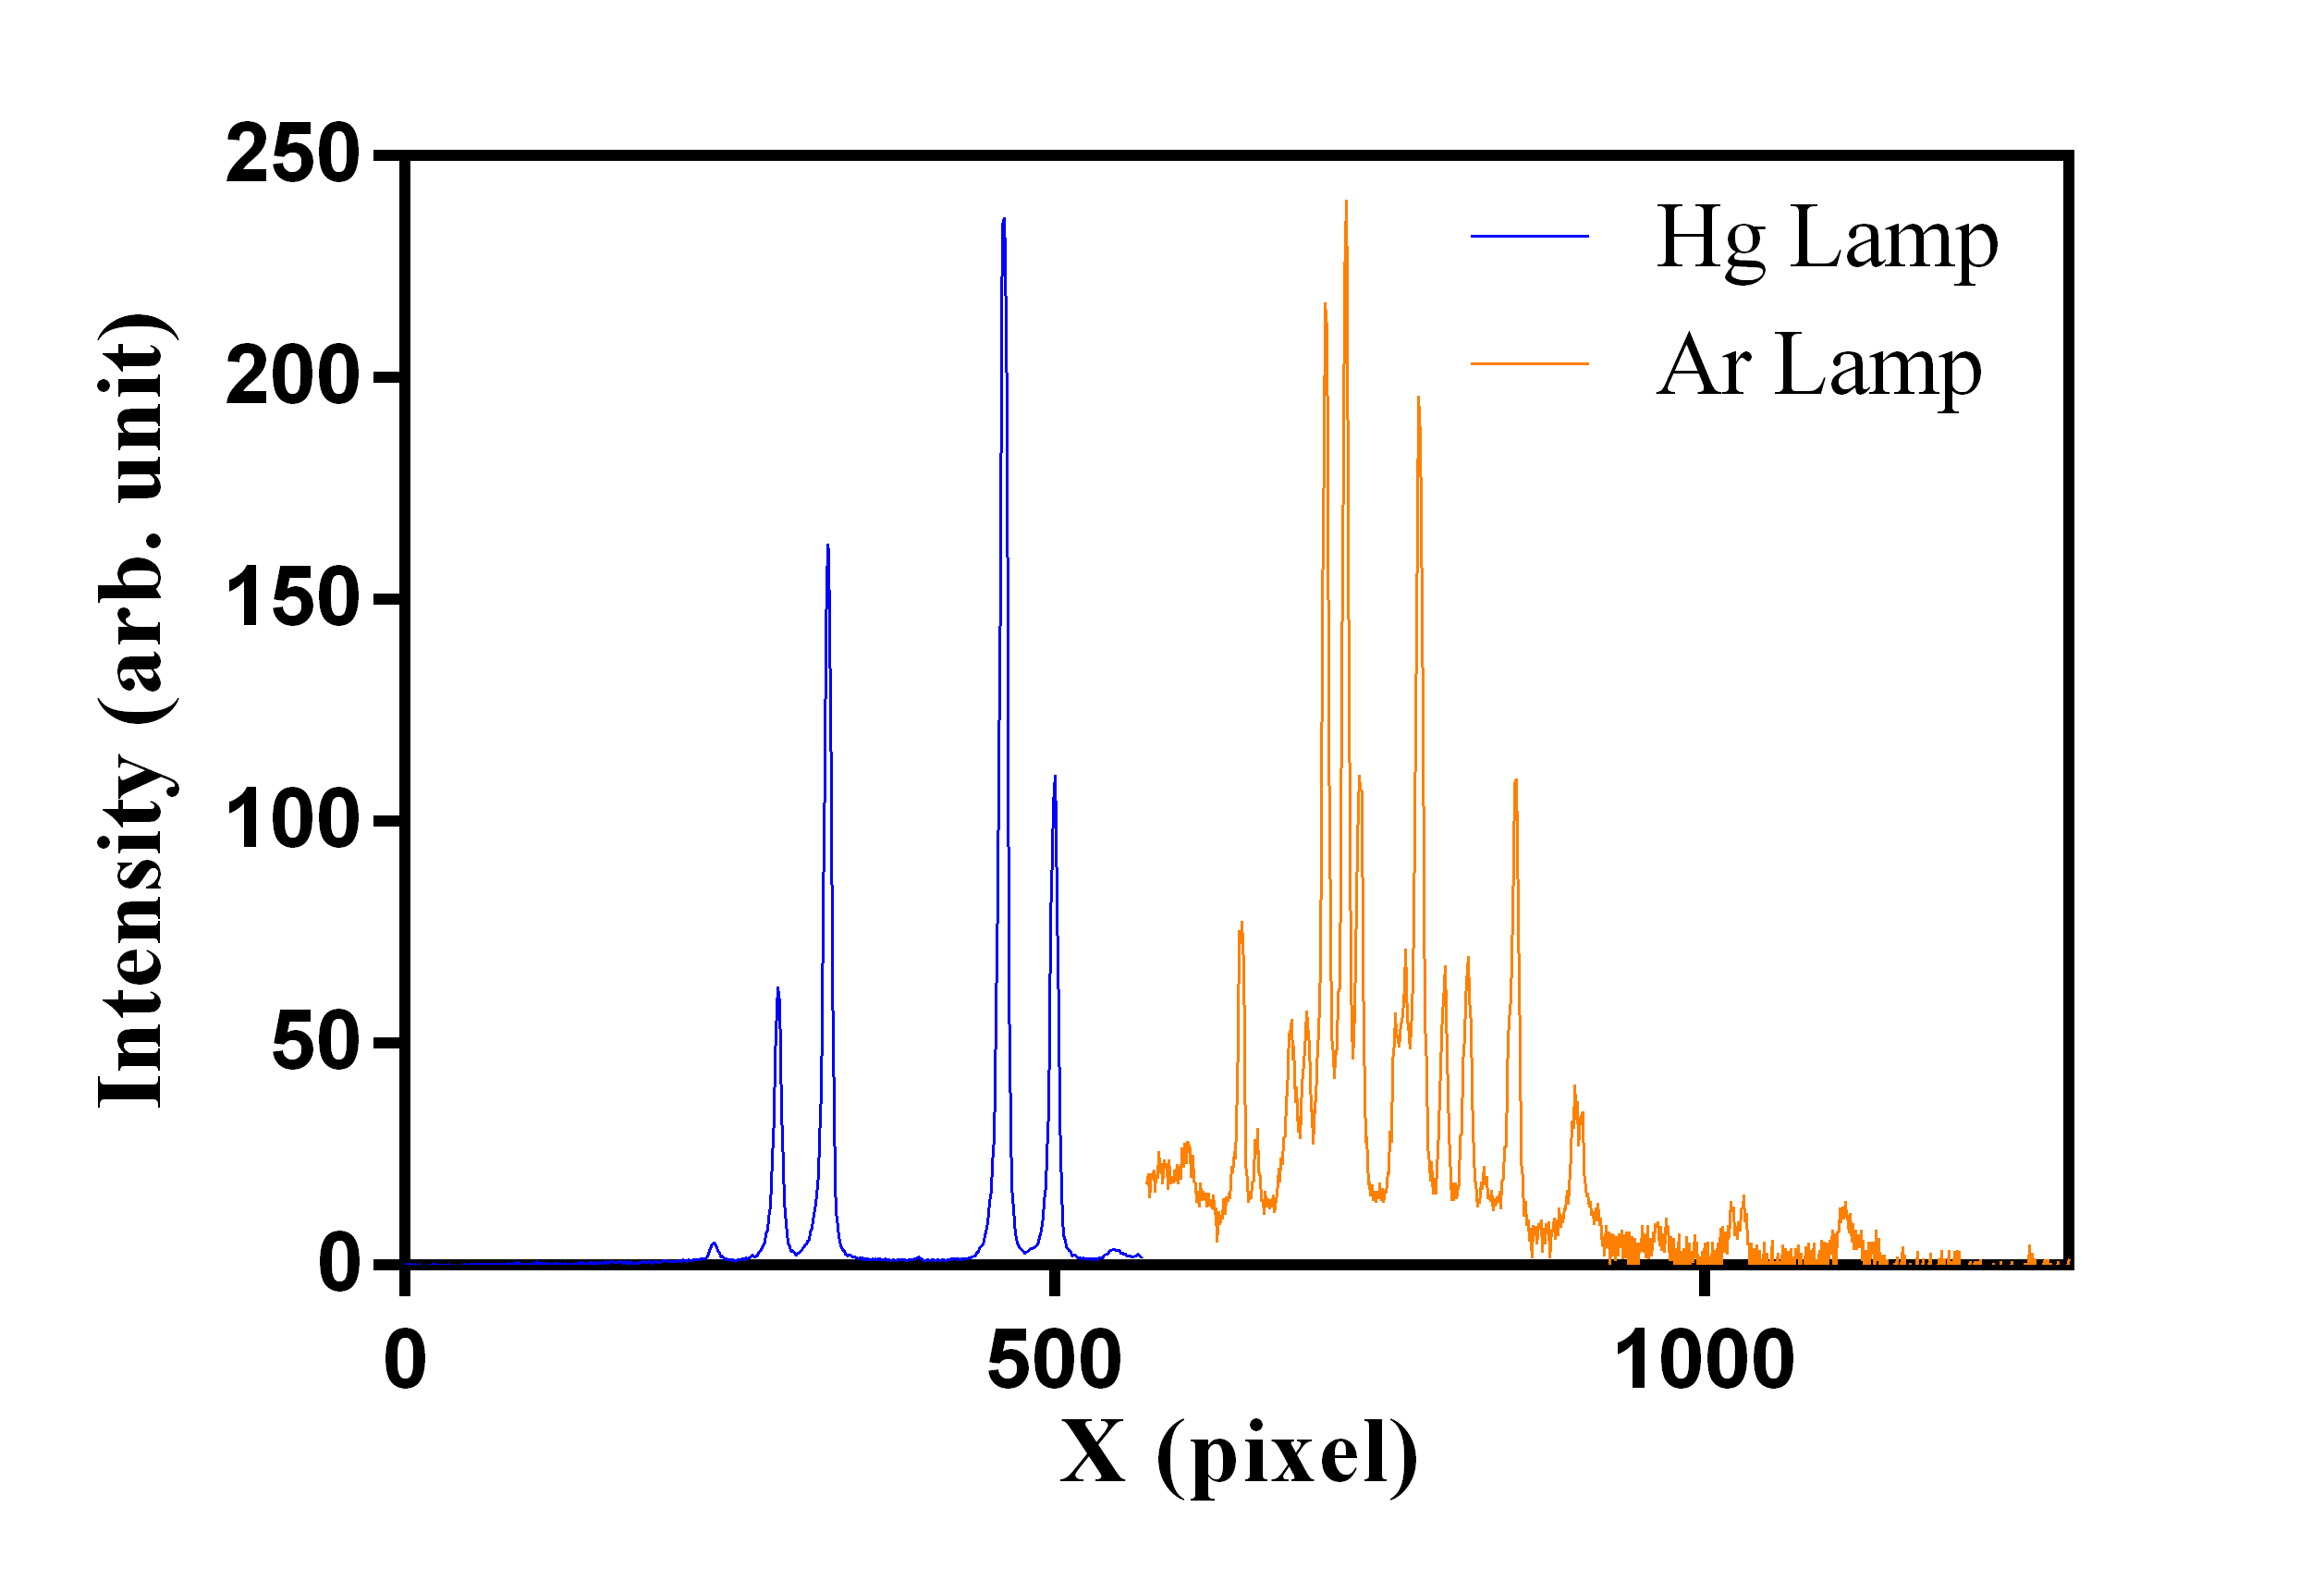
\includegraphics[width=15cm]{figures/Comebine_ArLamp.png} %插入图片,[]中设置图片大小,{}中是图片文件名
	\caption{氬燈數據AutoScaling並合併後光譜波形圖} %最终文档中希望显示的图片标题
	\label{氬燈數據AutoScaling並合併後光譜波形圖} %用于文内引用的标签
\end{figure}

波峰偵測時常以斜率\cite{slope-find-peak}作為判定方式,但因強度平衡後的汞氬燈數據也將造成氬燈區域雜訊被大幅放大,因此不宜將此數據用來以Hilbert Transform判定粗略波峰位置,故波峰偵測的第一步為將原始光譜數據進行Hilbert Transform,並找出所有轉換後的區域最大值與最小值如圖\ref{光譜經由希爾伯特轉換後的區域最大值與最小值位置}. 所示。
\begin{figure}[H] %H为当前位置,!htb为忽略美学标准,htbp为浮动图形
	\centering %图片居中
	\vspace{0.8cm}
	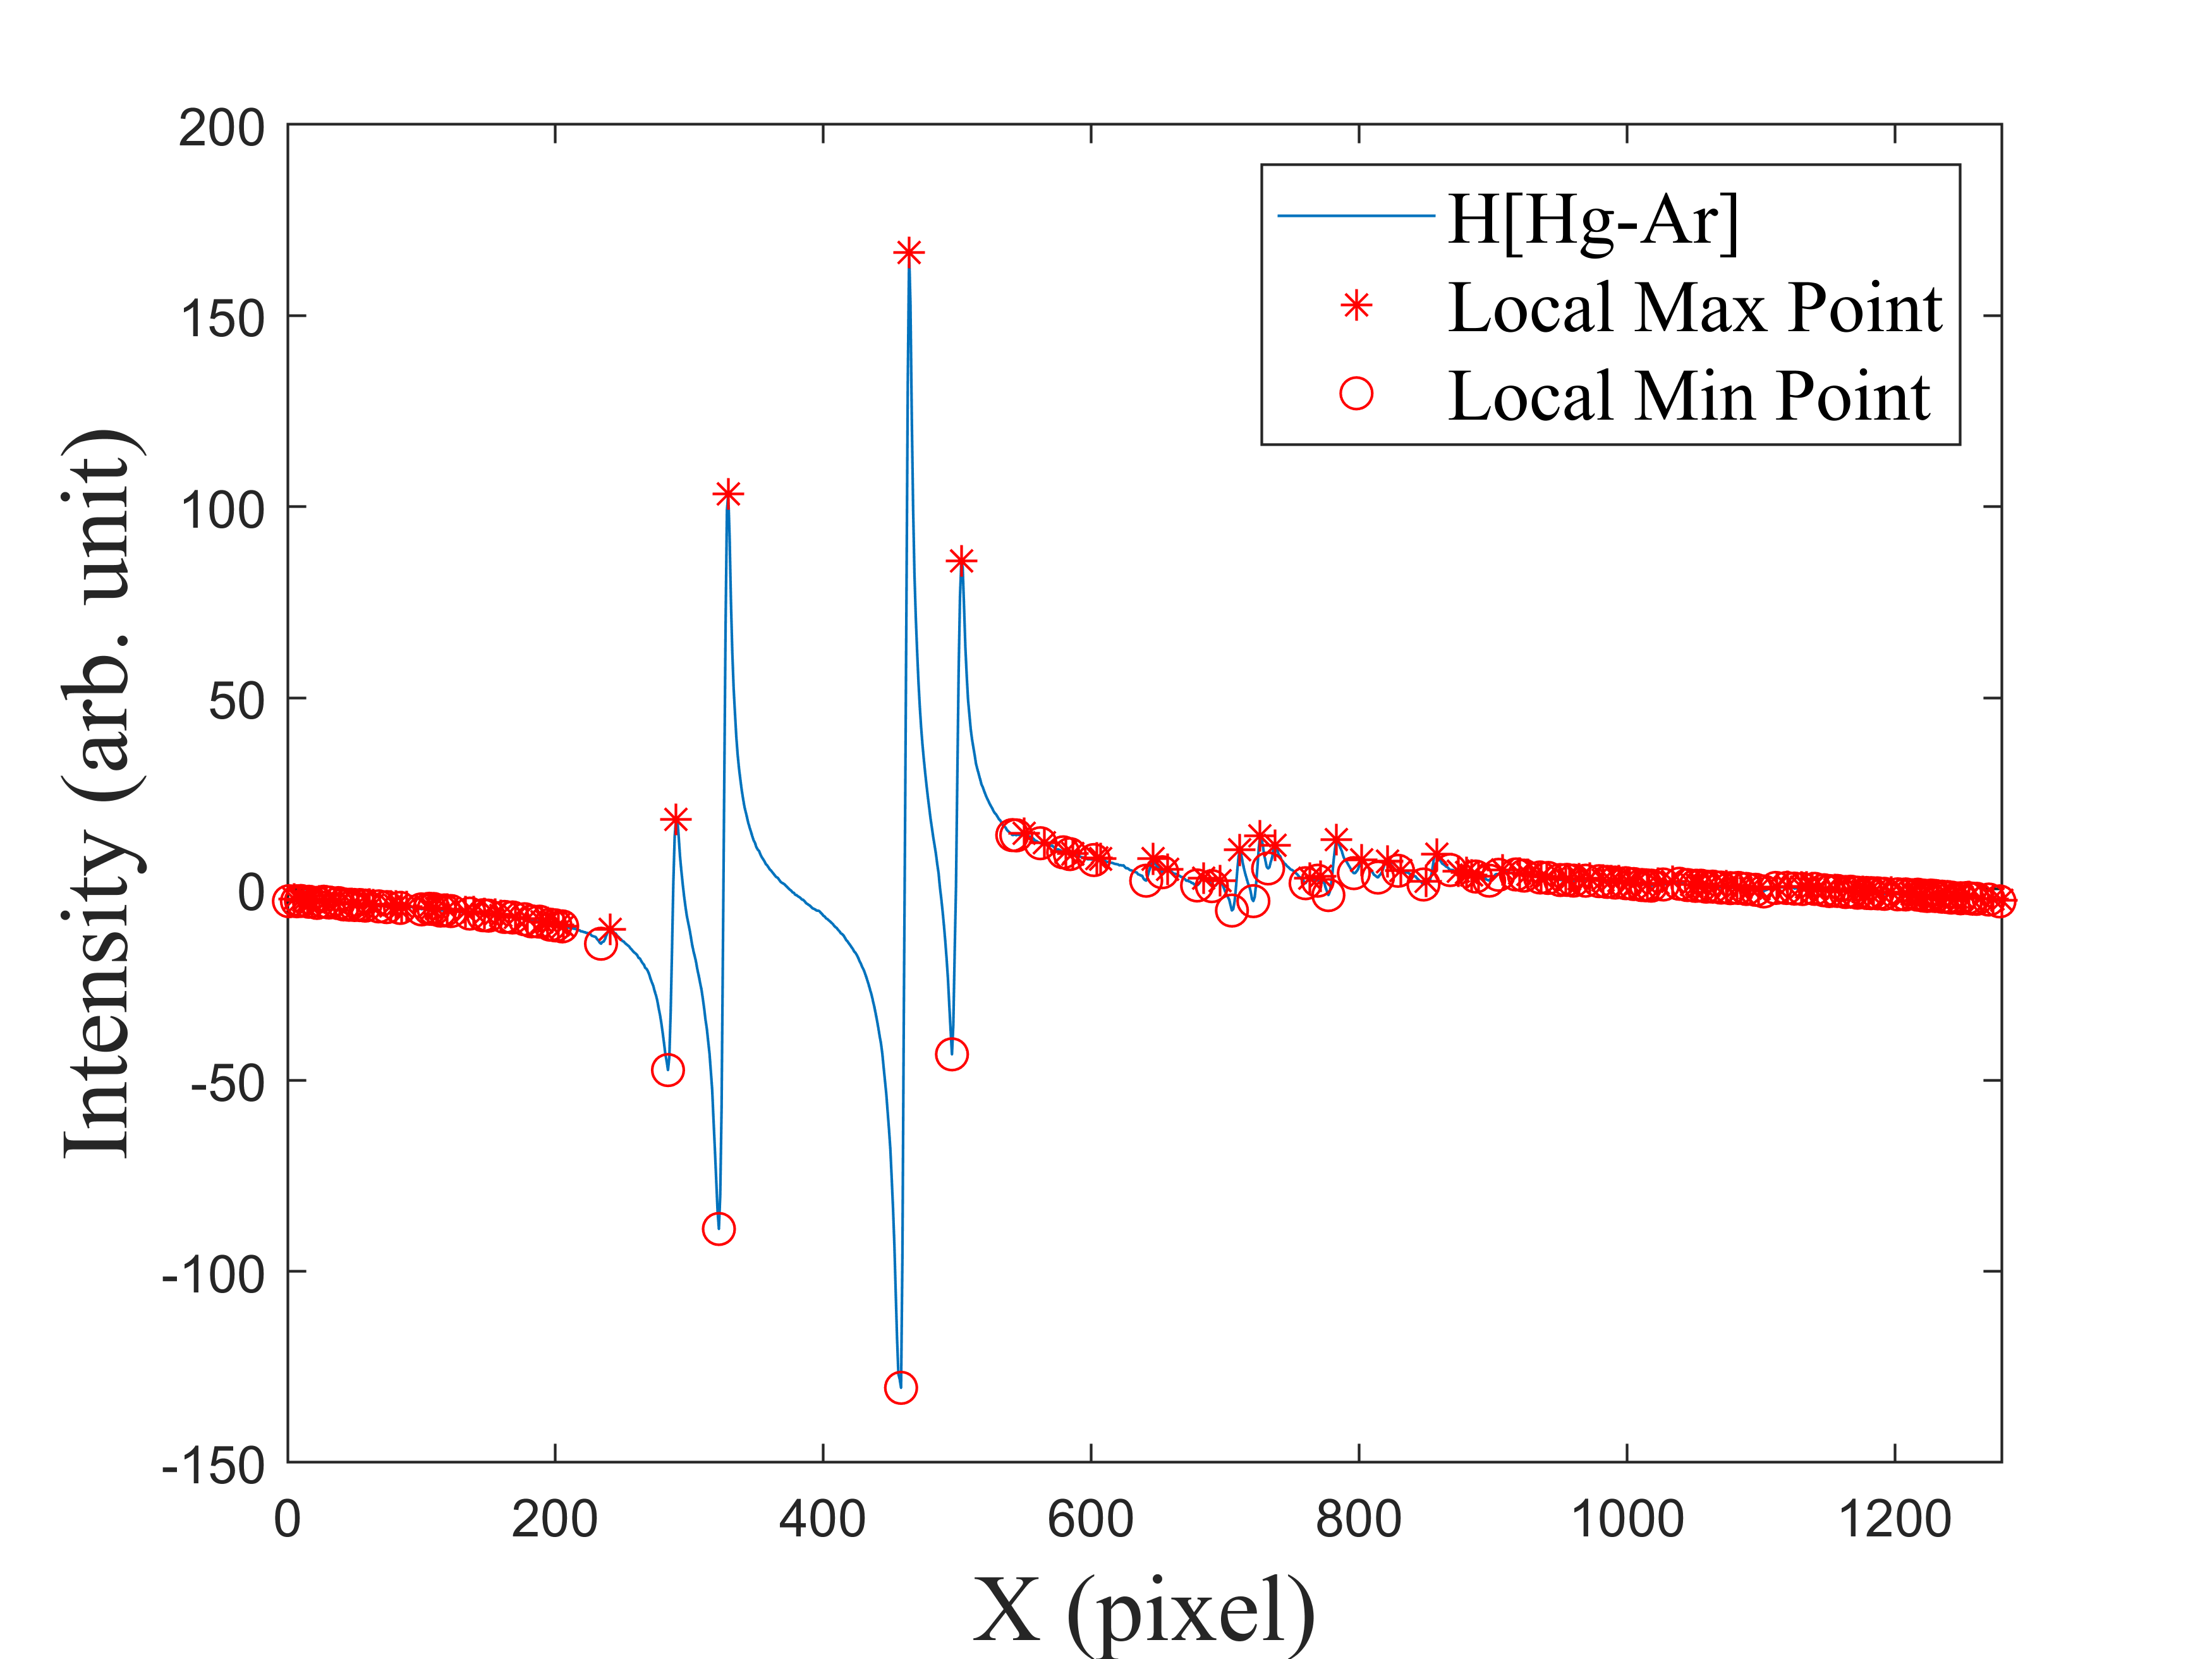
\includegraphics[width=\textwidth]{figures/Hil_HGAR_MAX_MIN.PNG} %插入图片,[]中设置图片大小,{}中是图片文件名
	\caption{原始光譜經由Hilbert Transform後的區域最大值與最小值位置} %最终文档中希望显示的图片标题
	\label{光譜經由希爾伯特轉換後的區域最大值與最小值位置} %用于文内引用的标签
\end{figure}
轉換後的波形數據之區域極值以斜率做為閥值,斜率大於閥值的上升線段中的最低點與最高點做為波峰偵測斜率判斷的特徵點。在滿足斜率閥值的線段中之與最低點與最高點之間,Hilbert Transform後的波峰位置落在兩者的中點,此點即為波峰預測位置,如圖\ref{滿足斜率線段之中點即為粗略峰值位置點}. 所示。並將估測出的峰值位置點實際與Hilbert Transform前原始光譜比較,如圖\ref{粗略峰值位置偵測}. 所示。
\begin{figure}[H] %H为当前位置,!htb为忽略美学标准,htbp为浮动图形
	\centering %图片居中
	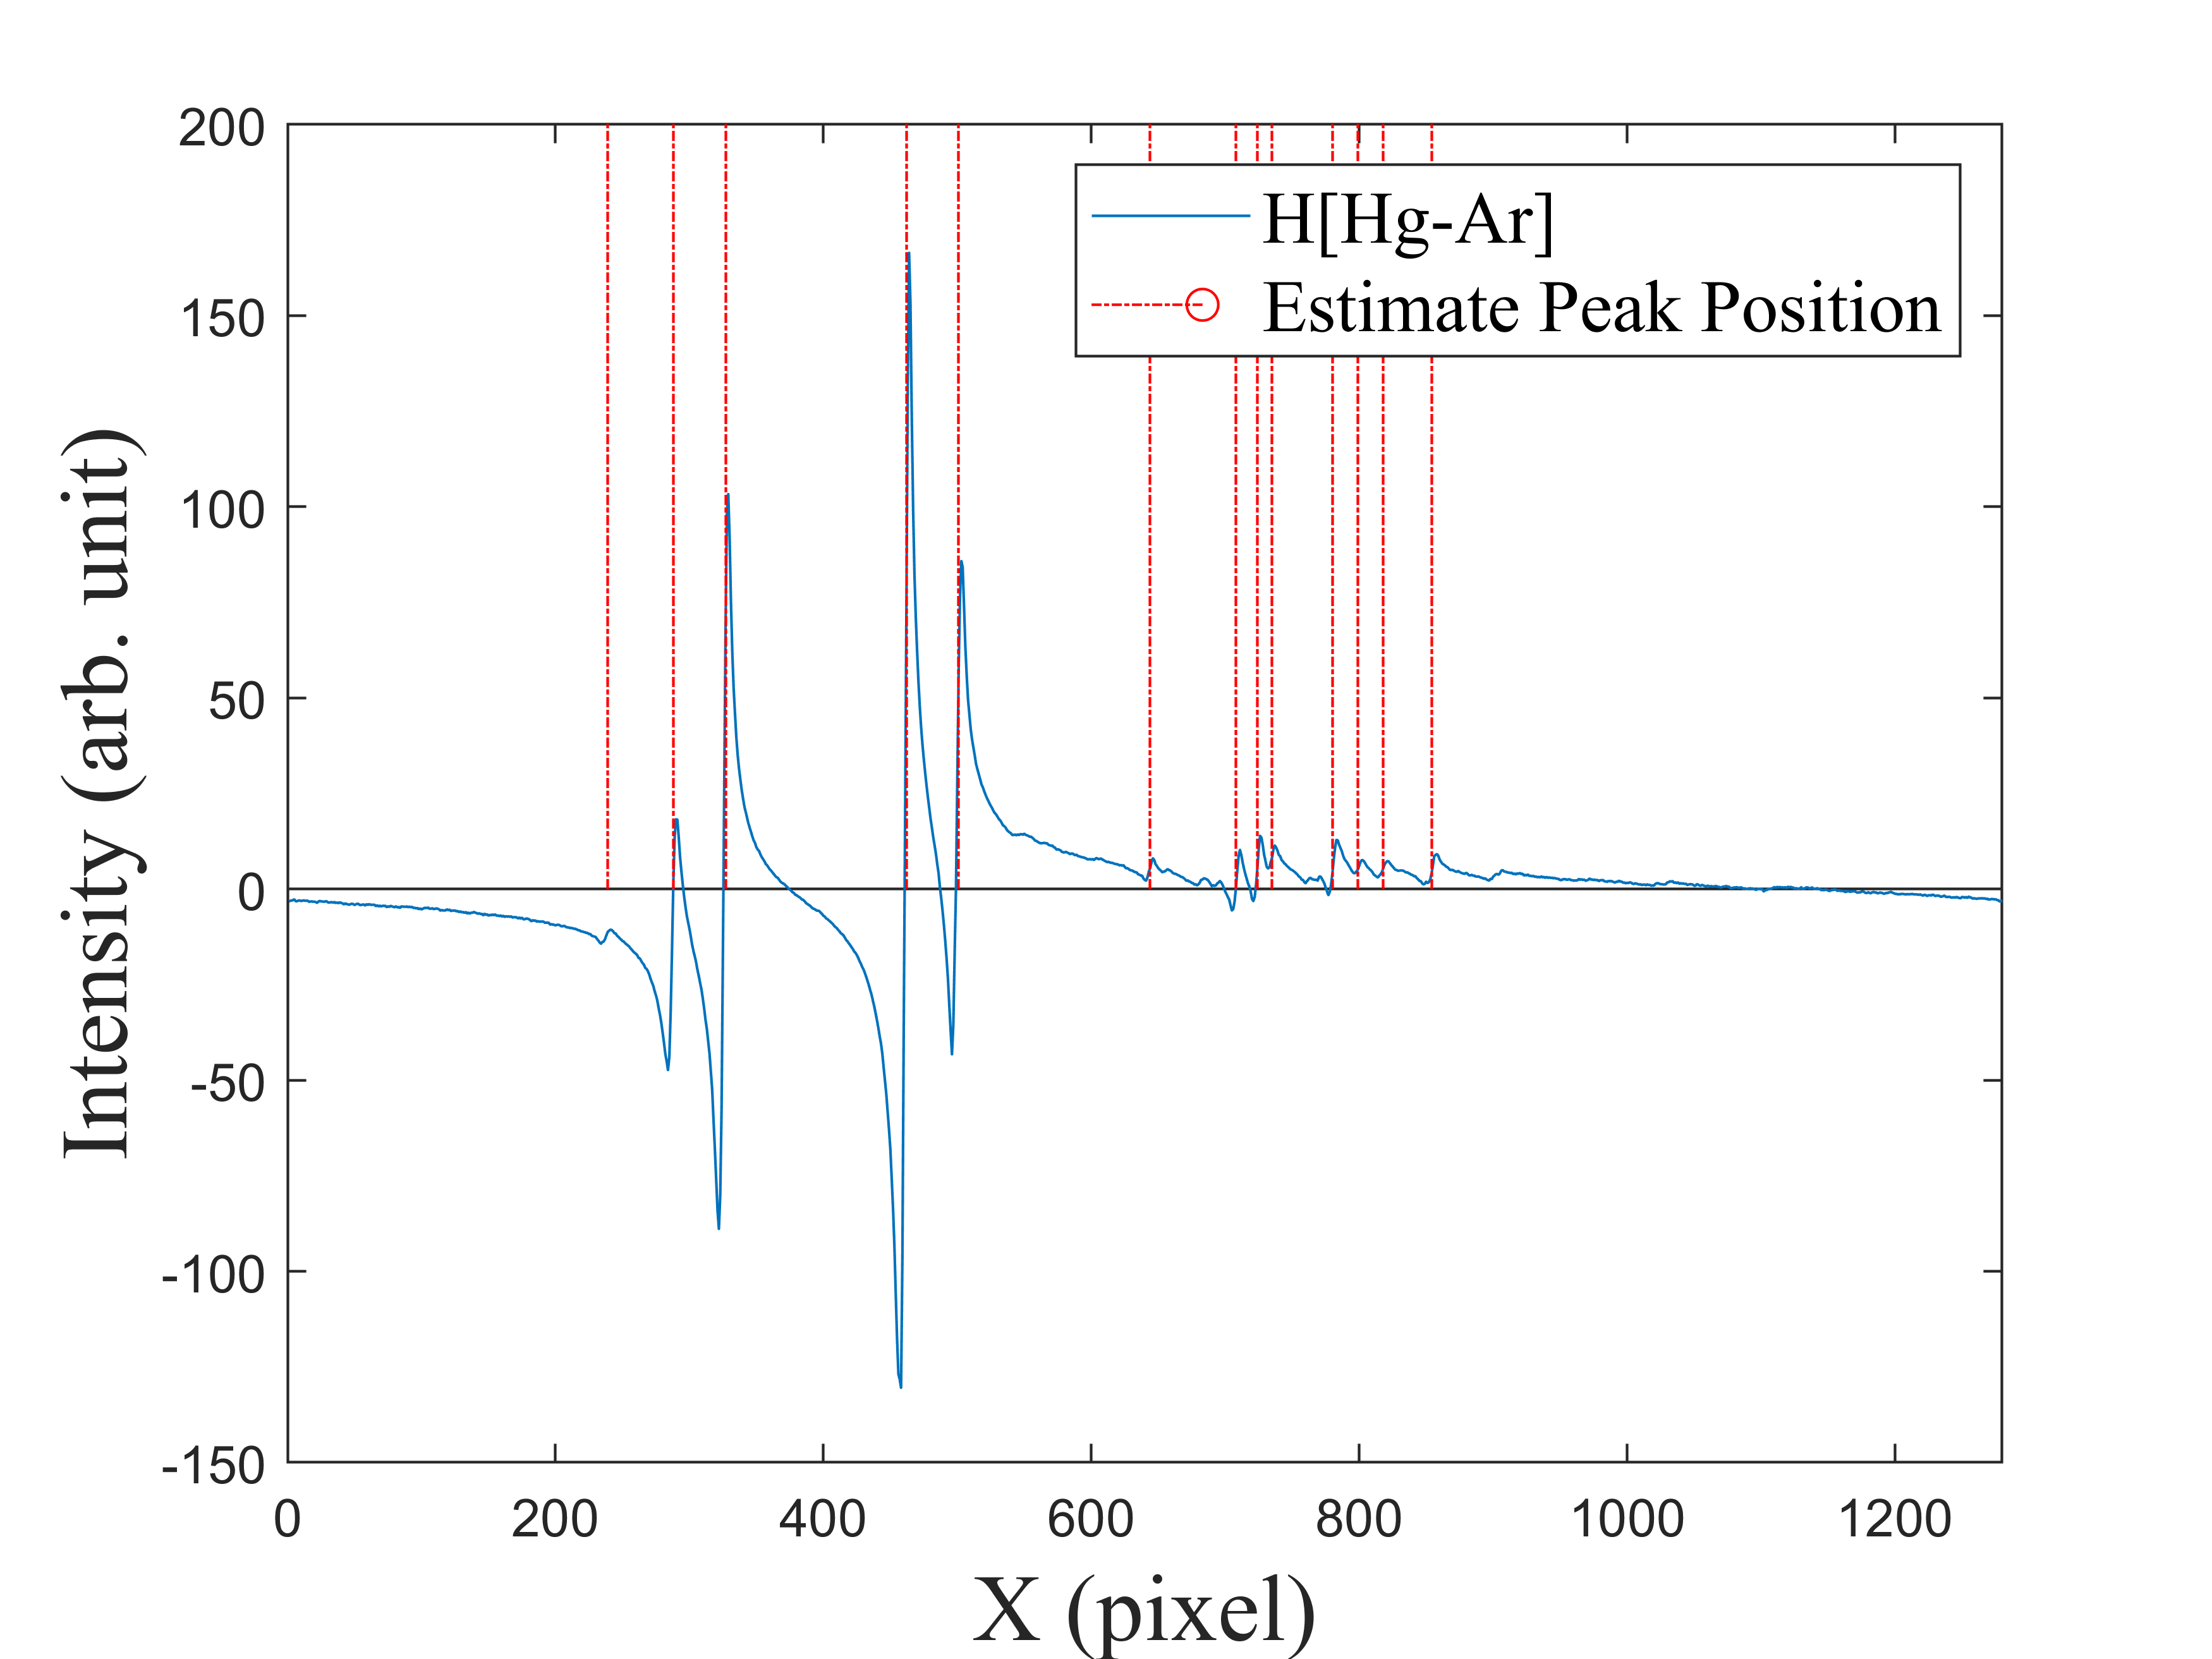
\includegraphics[width=14.5cm]{figures/estimate_peak_position.PNG} %插入图片,[]中设置图片大小,{}中是图片文件名
	\caption{滿足斜率線段之中點即為粗略峰值位置點} %最终文档中希望显示的图片标题
	\label{滿足斜率線段之中點即為粗略峰值位置點} %用于文内引用的标签
\end{figure}
\begin{figure}[H] %H为当前位置,!htb为忽略美学标准,htbp为浮动图形
	\centering %图片居中
	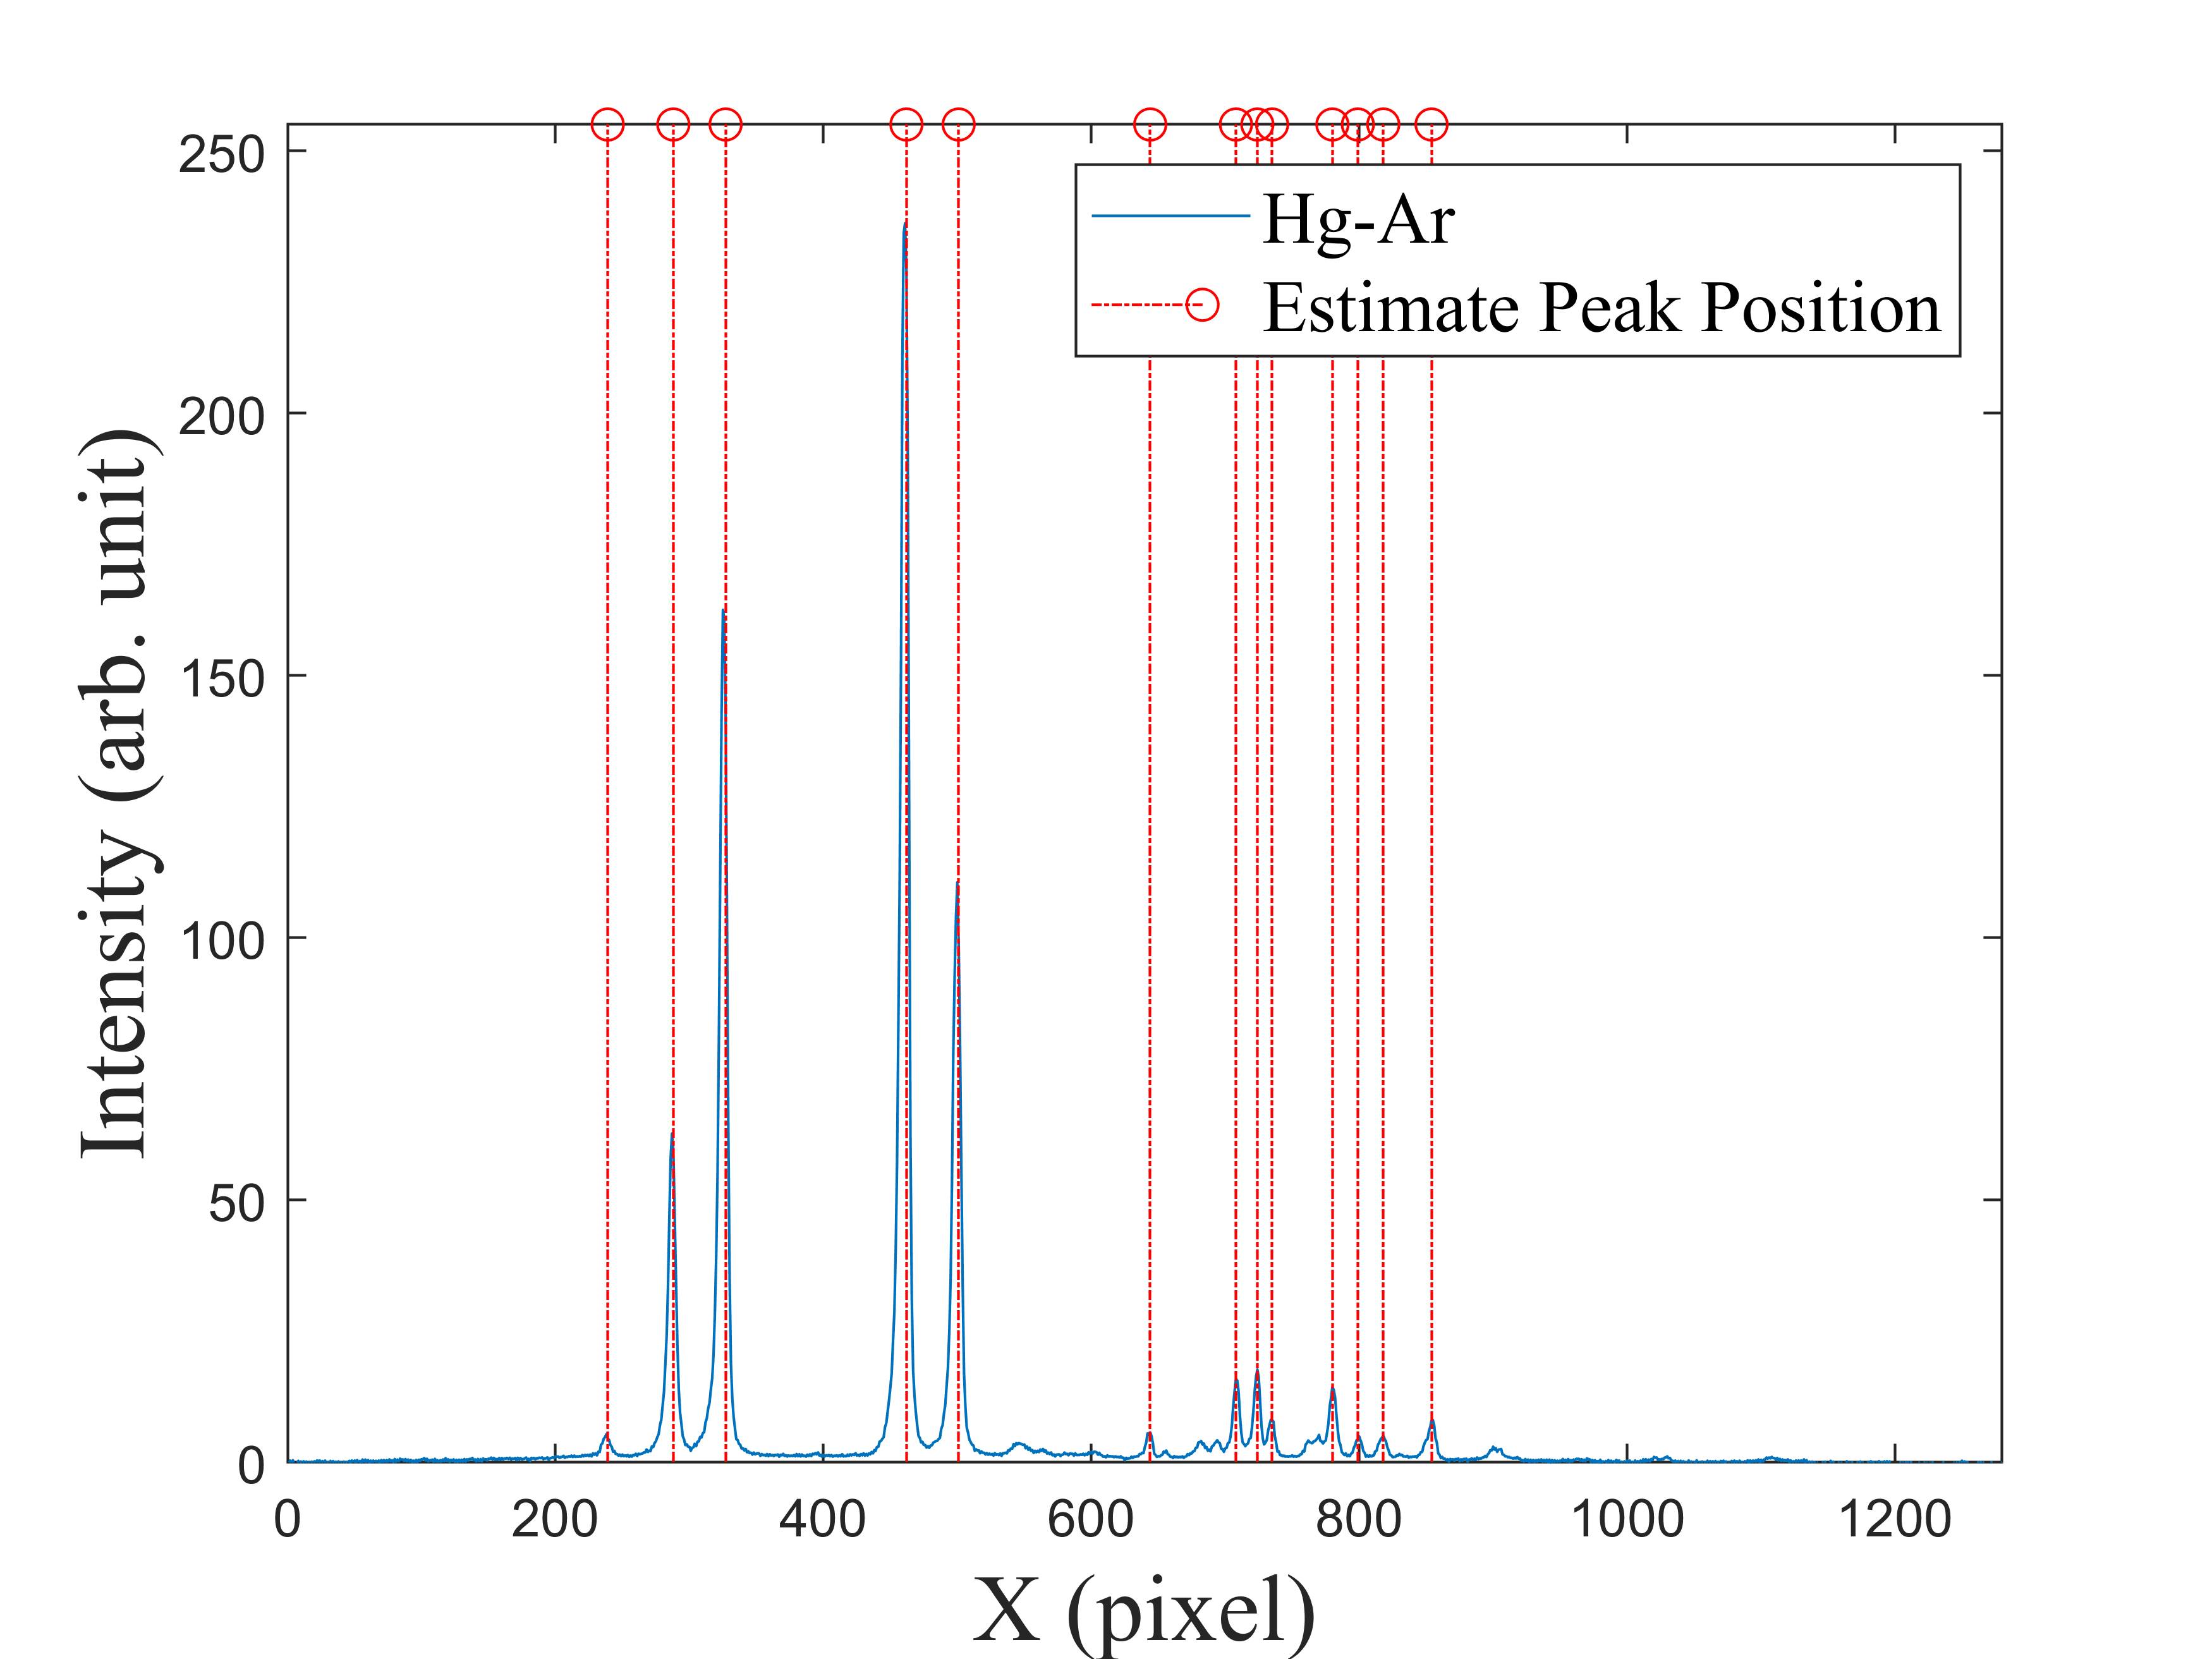
\includegraphics[width=14.5cm]{figures/估測峰值位置.PNG} %插入图片,[]中设置图片大小,{}中是图片文件名
	\caption{粗略峰值位置偵測} %最终文档中希望显示的图片标题
	\label{粗略峰值位置偵測} %用于文内引用的标签
\end{figure}
求得粗略峰值位置後,因應勞倫茲模型擬合需求,需要每一區域中僅有一個波峰,因此為了將數據進行區域分割,本文使用斜率反折法分割區域。
先找出強度平衡後數據的所有區域最大值與最小值,如圖\ref{平衡後汞氬燈波型數據所有區域最大值與最小值}. 所示,再將所有區域最大值與最小值的點由像素大小由小至大排列,再求出所有兩點間斜率,斜率急升前的點與急降後的點,代表為單一波峰的波型起始與結束點,取出所有滿足此斜率行為的點如圖\ref{平衡後汞氬燈波峰數據擬和區域分割點}. 所示。
\begin{figure}[H] %H为当前位置,!htb为忽略美学标准,htbp为浮动图形
	\centering %图片居中
	\vspace{0.8cm}
	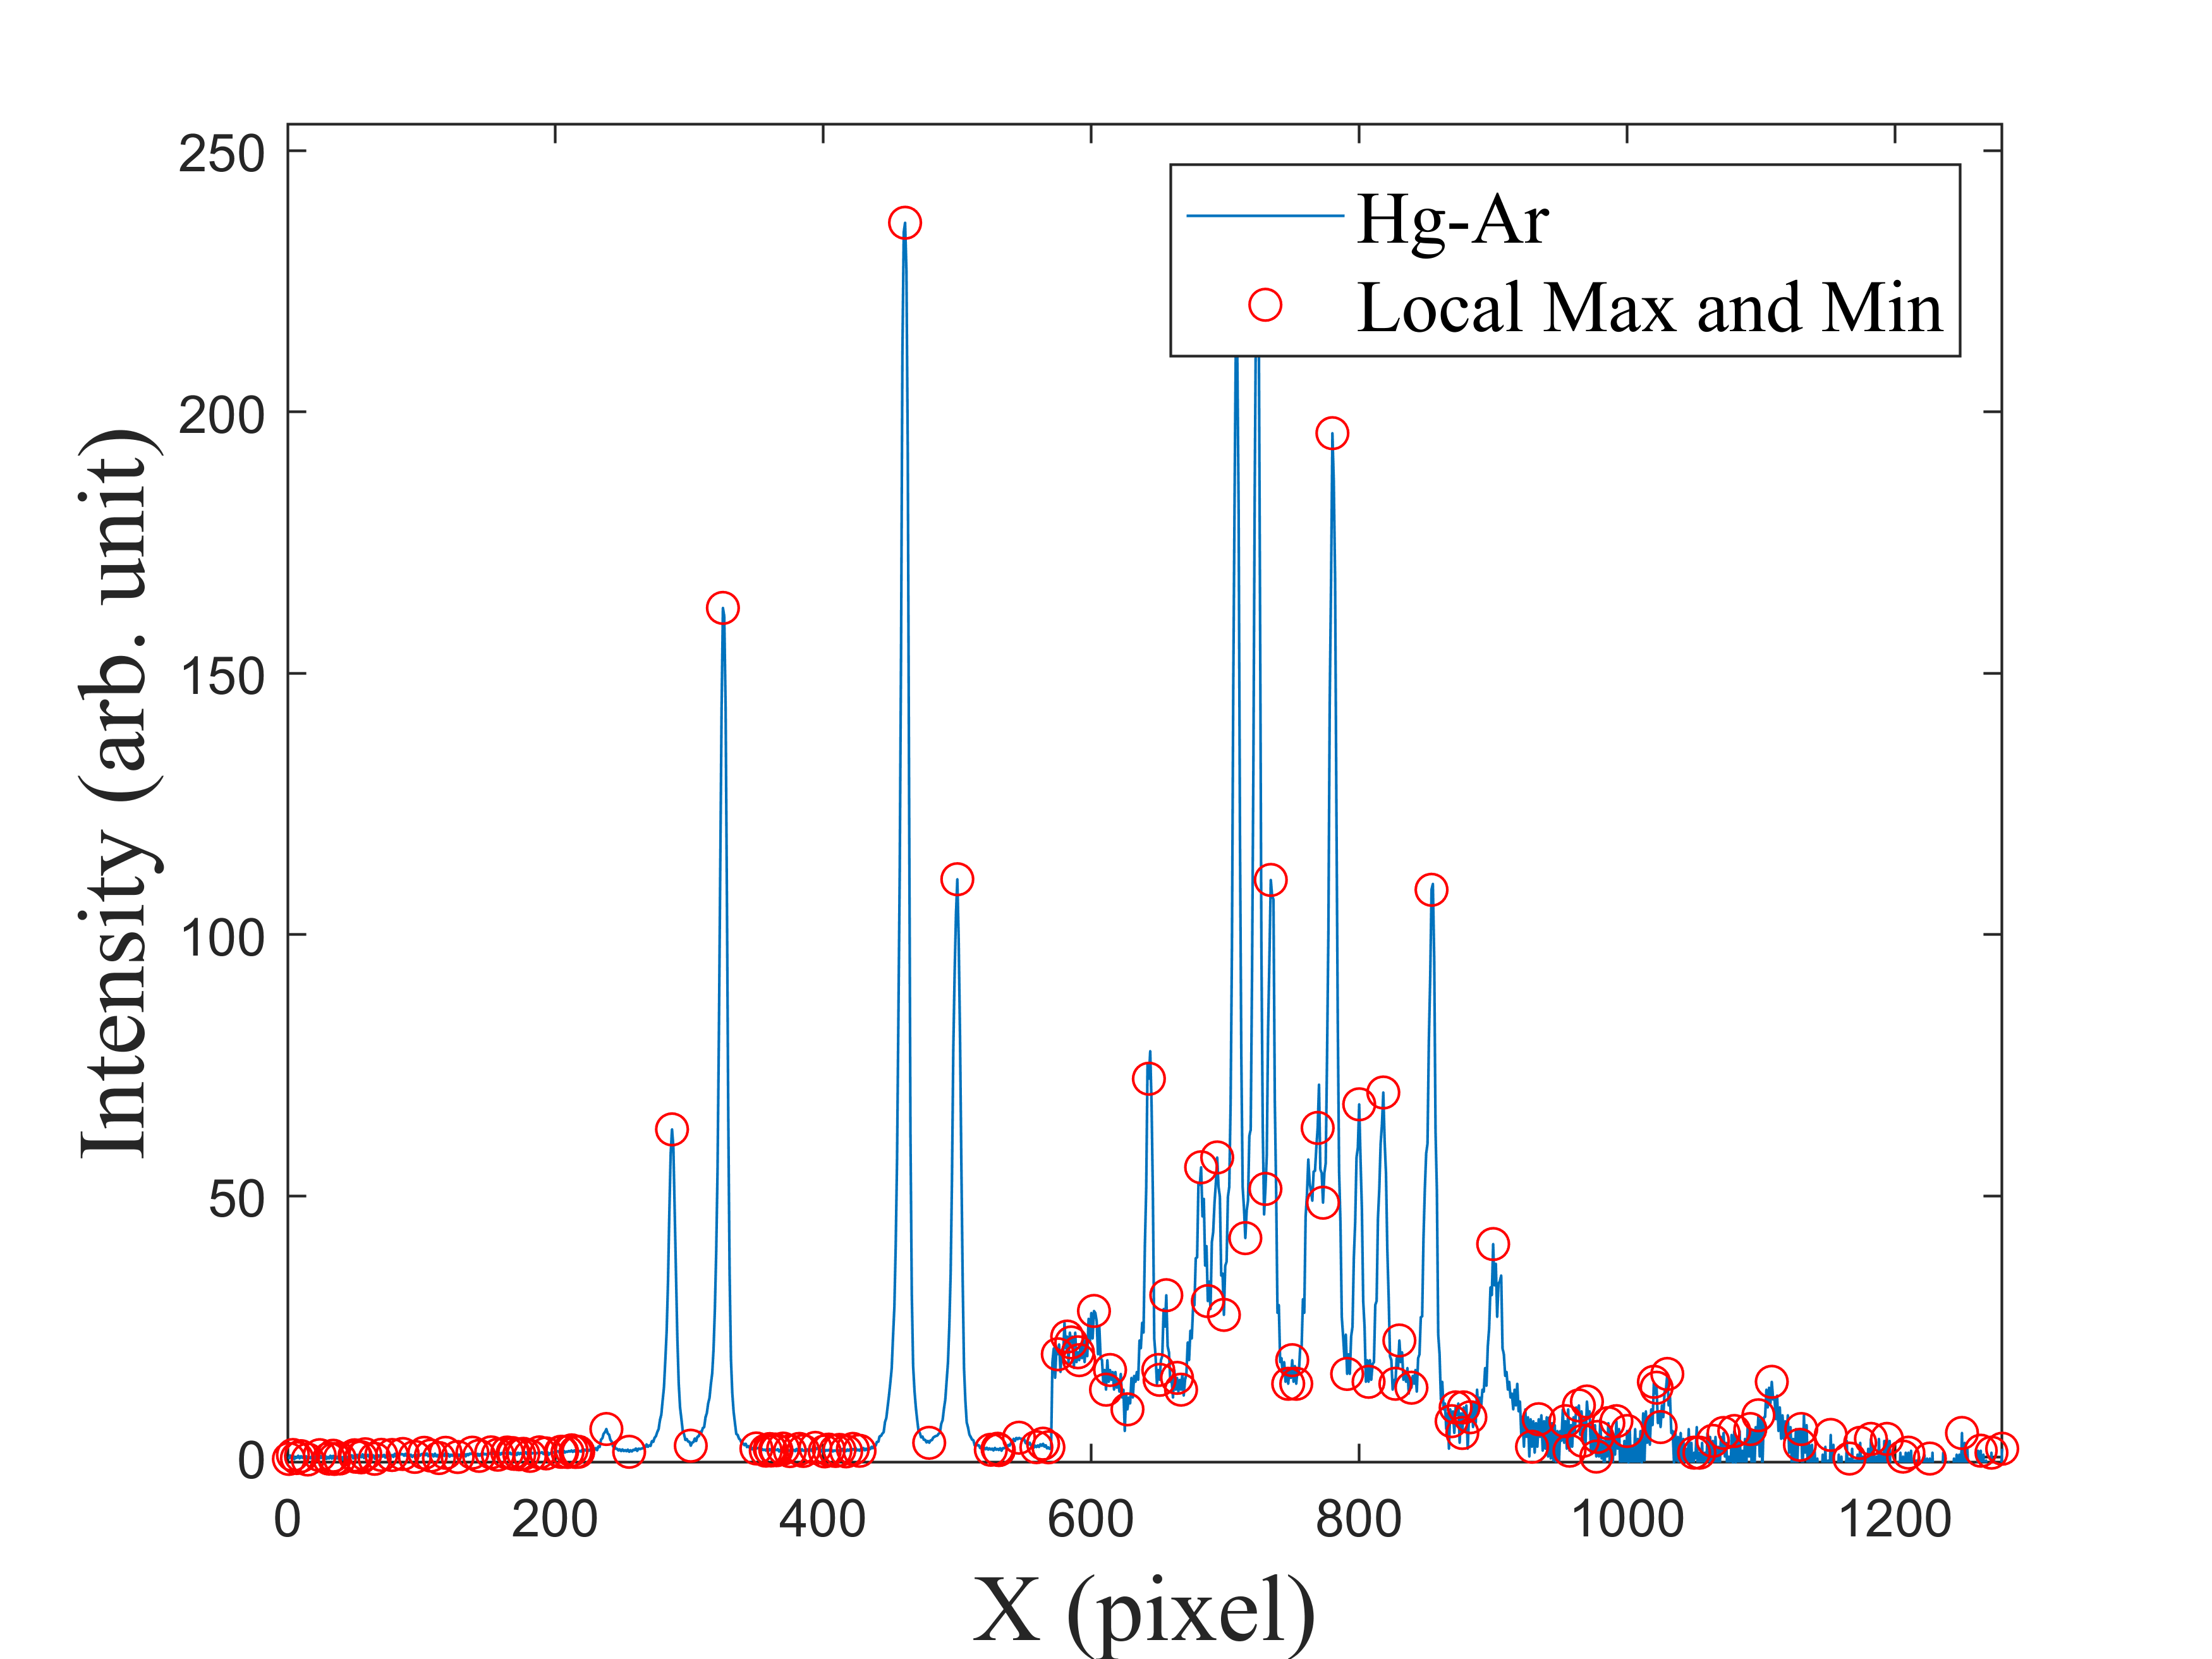
\includegraphics[width=16cm]{figures/combine_local_max_min.png} %插入图片,[]中设置图片大小,{}中是图片文件名
	\caption{平衡後汞氬燈波型數據所有區域最大值與最小值} %最终文档中希望显示的图片标题
	\label{平衡後汞氬燈波型數據所有區域最大值與最小值} %用于文内引用的标签
\end{figure}
\begin{figure}[H] %H为当前位置,!htb为忽略美学标准,htbp为浮动图形
	\centering %图片居中
	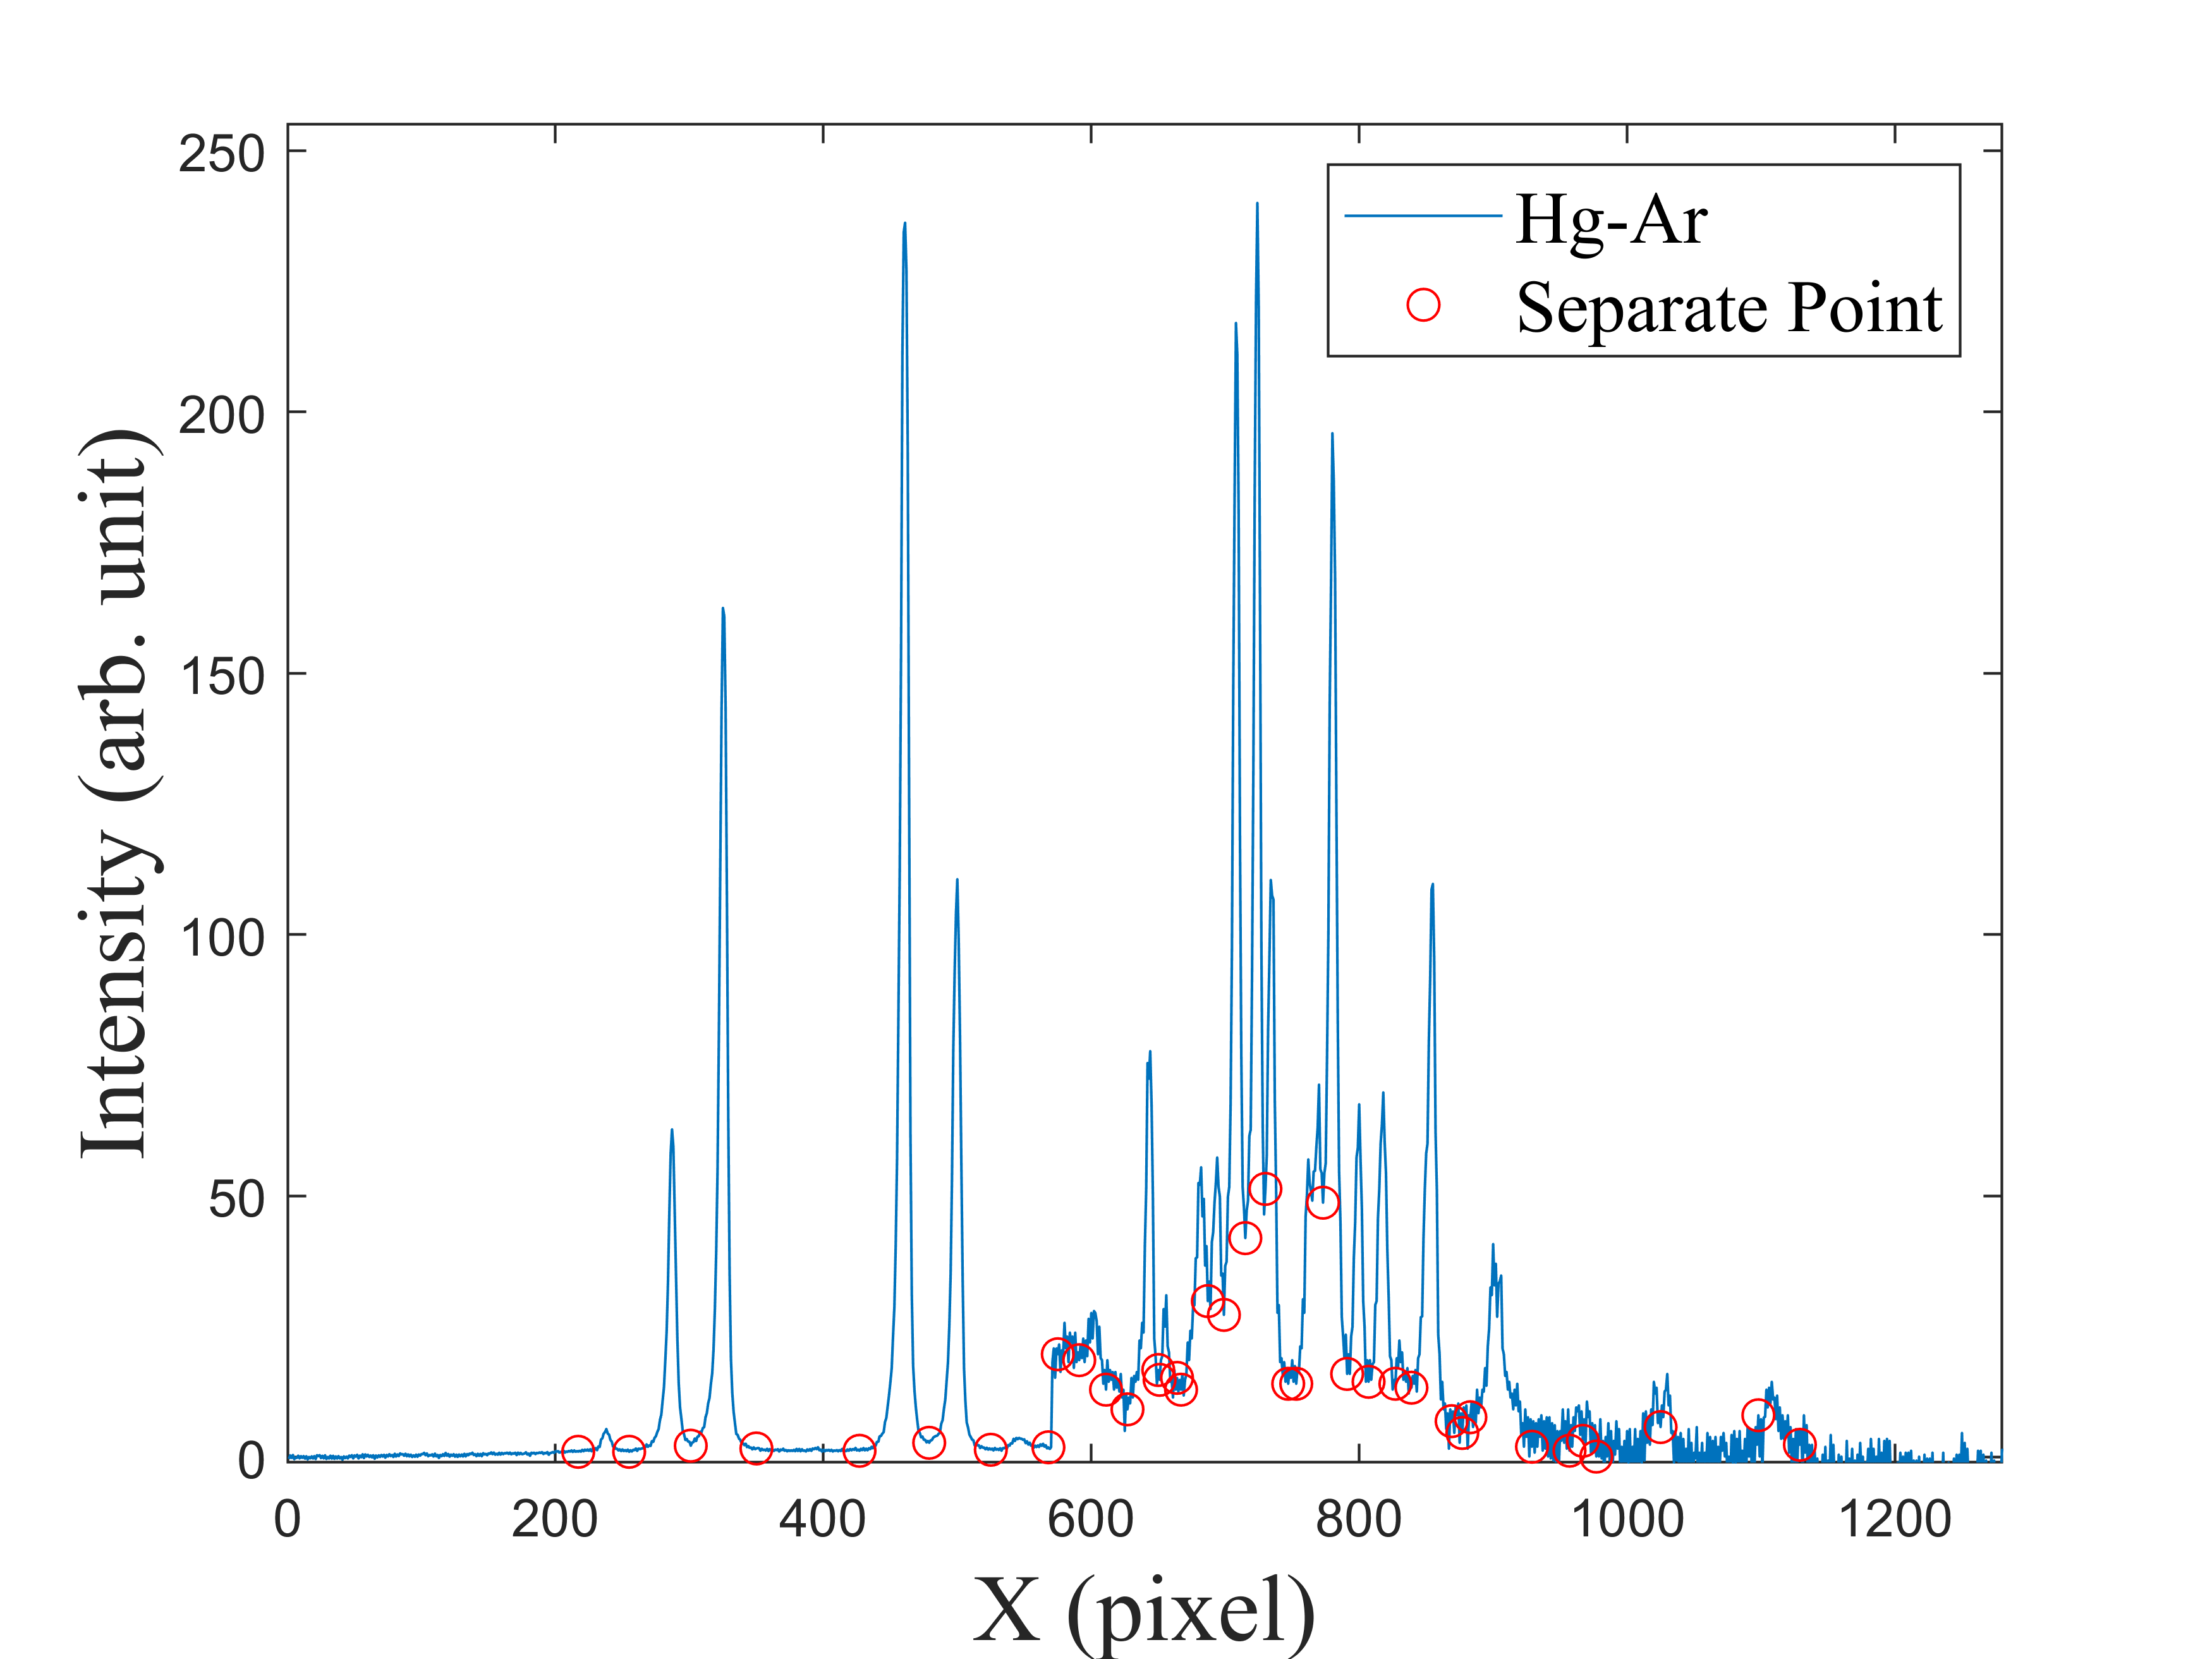
\includegraphics[width=16cm]{figures/combine_sep.png} %插入图片,[]中设置图片大小,{}中是图片文件名
	\caption{平衡後汞氬燈波峰數據擬和區域分割點} %最终文档中希望显示的图片标题
	\label{平衡後汞氬燈波峰數據擬和區域分割點} %用于文内引用的标签
\end{figure}
\par
以這些圖\ref{平衡後汞氬燈波峰數據擬和區域分割點}. 中所求出的分割點對數據進行分割後,如圖\ref{平衡後汞氬燈波峰數據擬和區域分割}. 所示。雖然分割後的分割區域中,並非所有區域數據皆能夠以模型擬合,但含有波峰數據的區域經過數據分割後,滿足第二章所提到模型擬合所需要之先前條件與準備,即所有分割區域中的波峰數據僅剩餘一個波峰,再對分割後區域內數據各自以勞倫茲模型擬合\cite{Lorentz-0},擬合後結果如圖\ref{區域分割後數據以勞倫茲模型擬合結果圖}. 所示。
\begin{figure}[H] %H为当前位置,!htb为忽略美学标准,htbp为浮动图形
	\centering %图片居中
	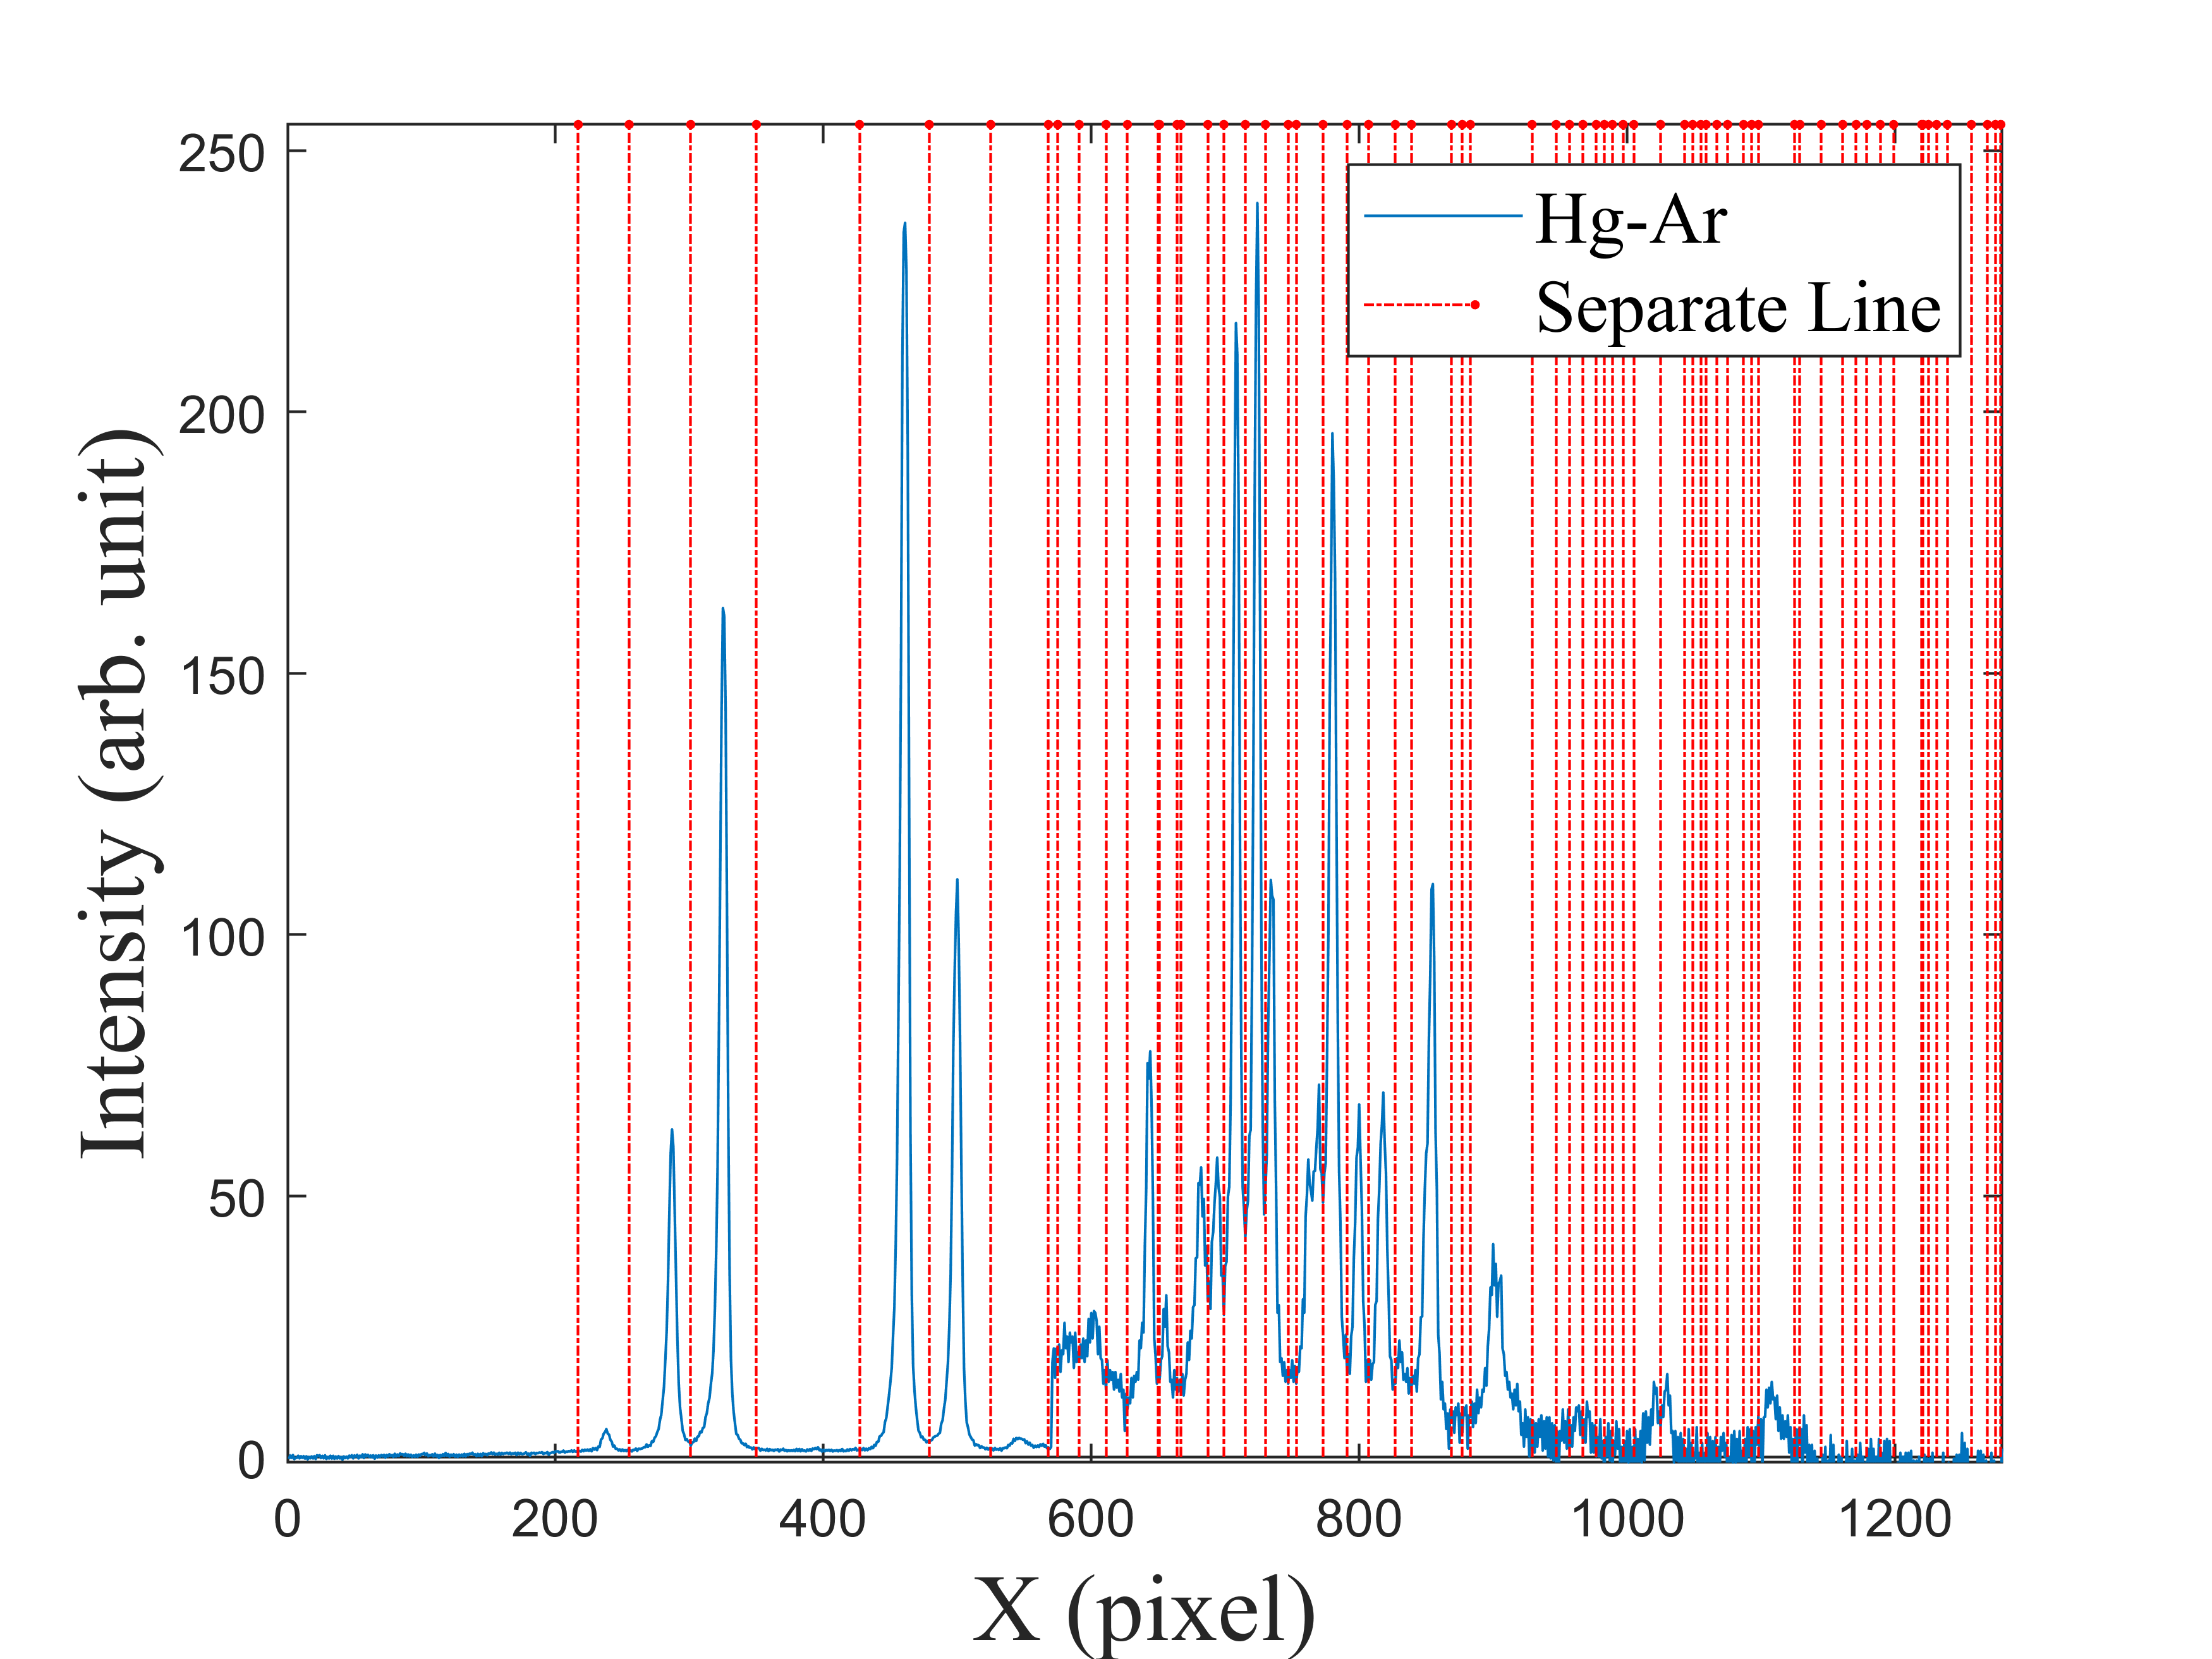
\includegraphics[width=14.5cm]{figures/combine_sep_line600.png} %插入图片,[]中设置图片大小,{}中是图片文件名
	\caption{平衡後汞氬燈波峰數據擬和區域分割} %最终文档中希望显示的图片标题
	\label{平衡後汞氬燈波峰數據擬和區域分割} %用于文内引用的标签
\end{figure}

\begin{figure}[H] %H为当前位置,!htb为忽略美学标准,htbp为浮动图形
	\centering %图片居中
	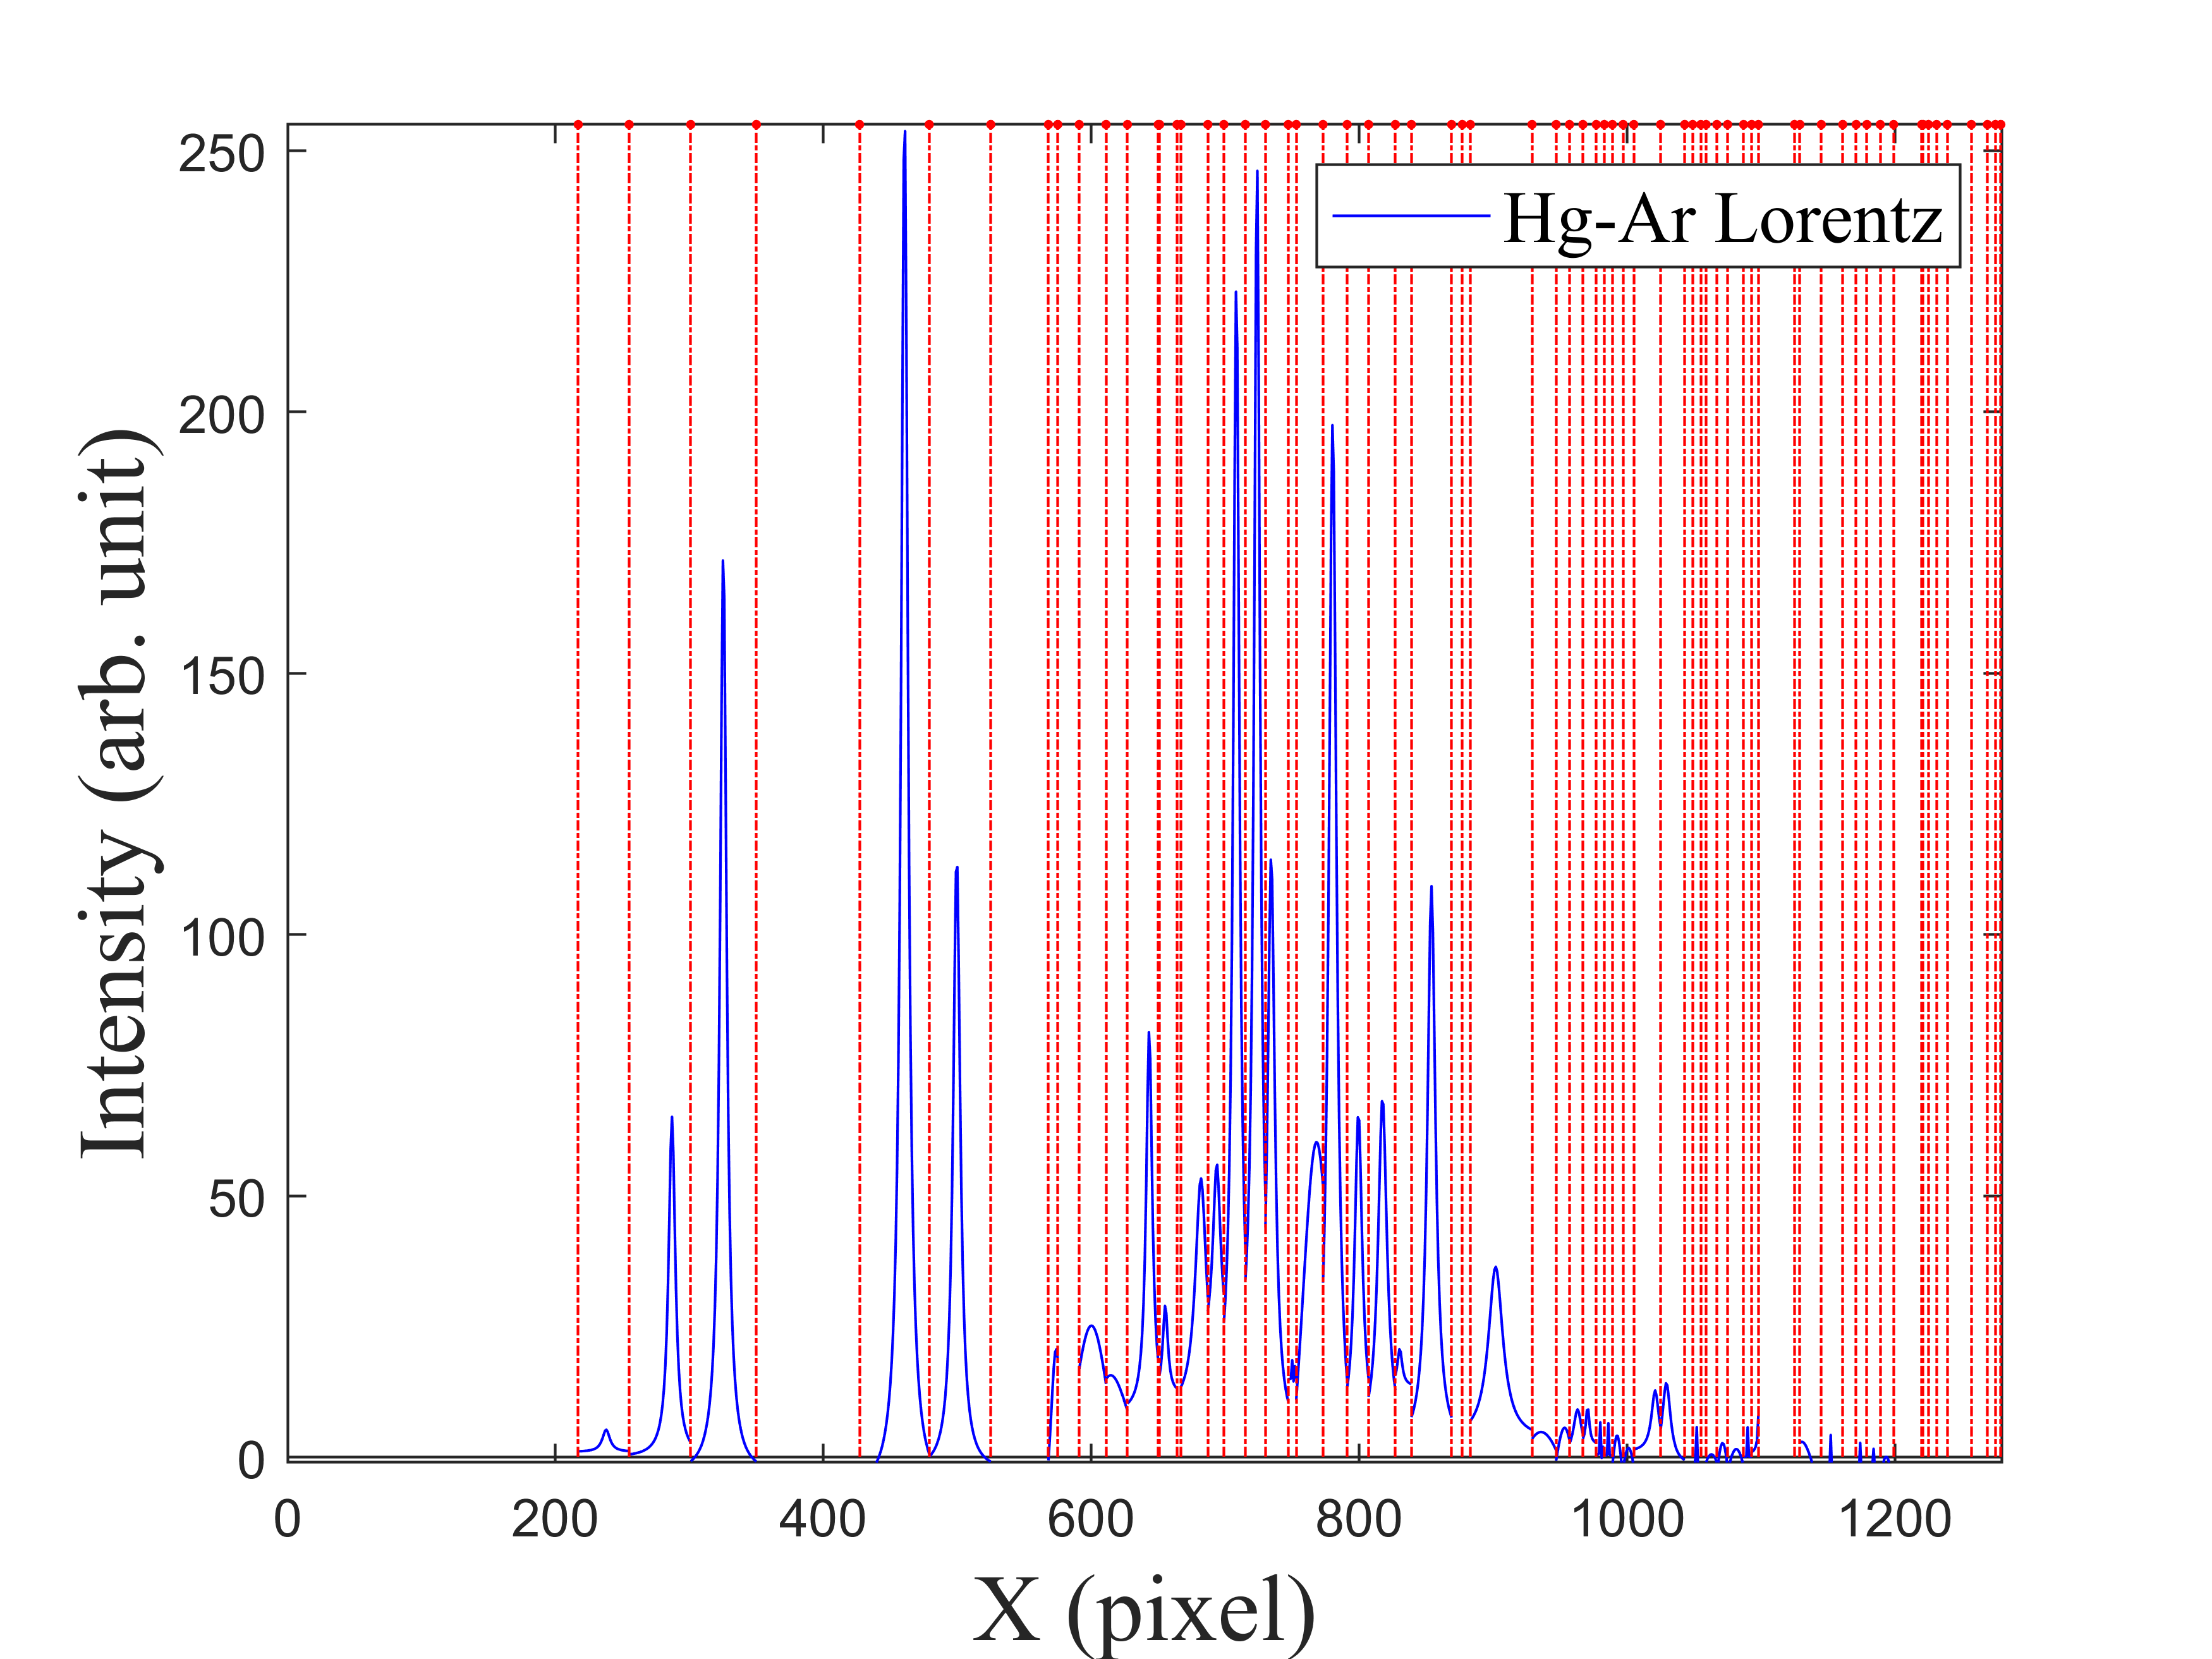
\includegraphics[width=14.5cm]{figures/comebine_hg_ar_lorent.png} %插入图片,[]中设置图片大小,{}中是图片文件名
	\caption{區域分割後數據以勞倫茲模型擬合結果圖} %最终文档中希望显示的图片标题
	\label{區域分割後數據以勞倫茲模型擬合結果圖} %用于文内引用的标签
\end{figure}
再將擬合後獲得的勞倫茲模型參數計算,並將找出的每一個區域中波峰精確的位置,其在勞倫茲模型中的強度,標示於圖\ref{區域分割後數據以勞倫茲模型擬合後且標示出精確波峰位置結果圖}. 中。
\begin{figure}[H] %H为当前位置,!htb为忽略美学标准,htbp为浮动图形
	\centering %图片居中
	\vspace{0.8cm}
	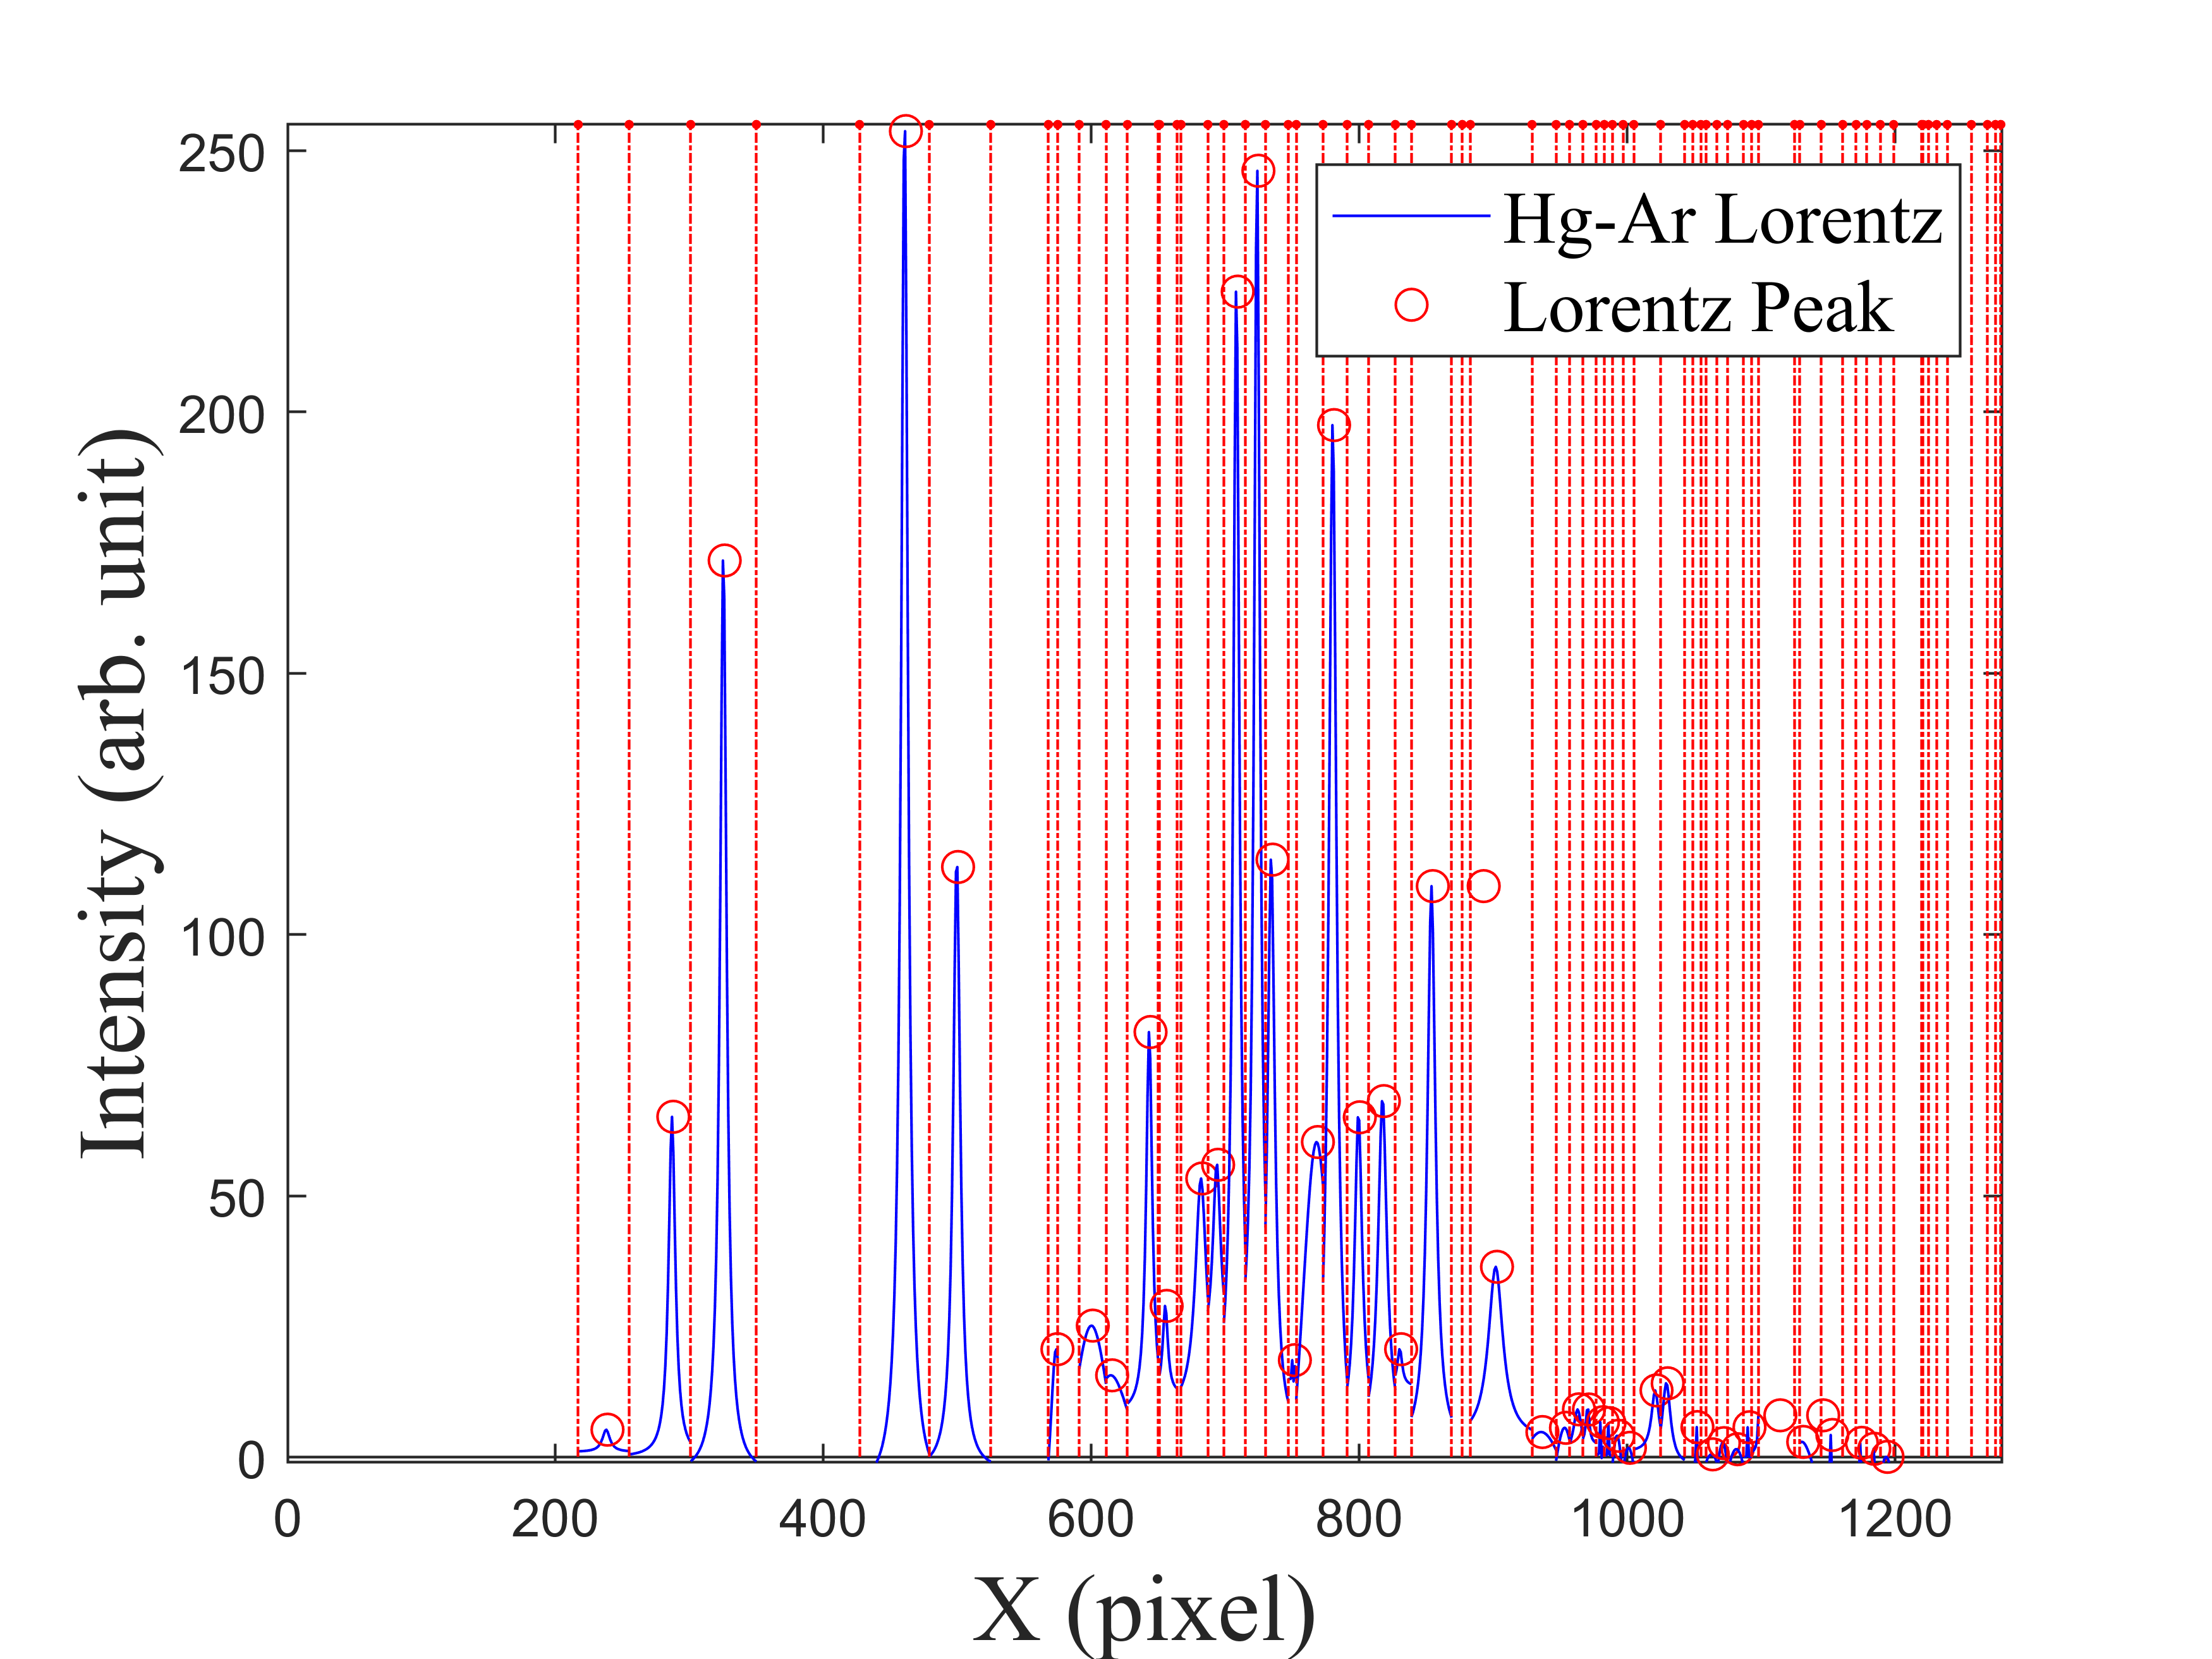
\includegraphics[width=15cm]{figures/comebine_hg_ar_lorent_with_peak.png} %插入图片,[]中设置图片大小,{}中是图片文件名
	\caption{區域分割後數據以勞倫茲模型擬合後且標示出精確波峰位置結果圖} %最终文档中希望显示的图片标题
	\label{區域分割後數據以勞倫茲模型擬合後且標示出精確波峰位置結果圖} %用于文内引用的标签
\end{figure}
由圖\ref{區域分割後數據以勞倫茲模型擬合後且標示出精確波峰位置結果圖}. 中可以看出,因氬燈區域數據強度平衡所造成雜訊放大因素,使得有些雜訊也滿足斜率閥值而被劃分進擬和區域,但由於不是所有數據皆能使用勞倫茲模型函數進行數據擬和,因此造成波峰位置與強度明顯不符合的峰值點,以下稱為無效峰值點,為了移除這些無效峰值點,與雜訊的峰值點,將圖\ref{滿足斜率線段之中點即為粗略峰值位置點}. 中透過原始汞氬燈光譜所找出的粗略峰值位置進行比對,將距離預測峰值最近的峰值點視為有效波峰,其餘波峰皆為無效峰值點,再剔除後所保留下的峰值位置與強度圖於平衡後光譜數據上表示,如圖\ref{區域分割後數據剔除無效峰值點後精確波峰位置結果圖}. 所示。
\begin{figure}[H] %H为当前位置,!htb为忽略美学标准,htbp为浮动图形
	\centering %图片居中
	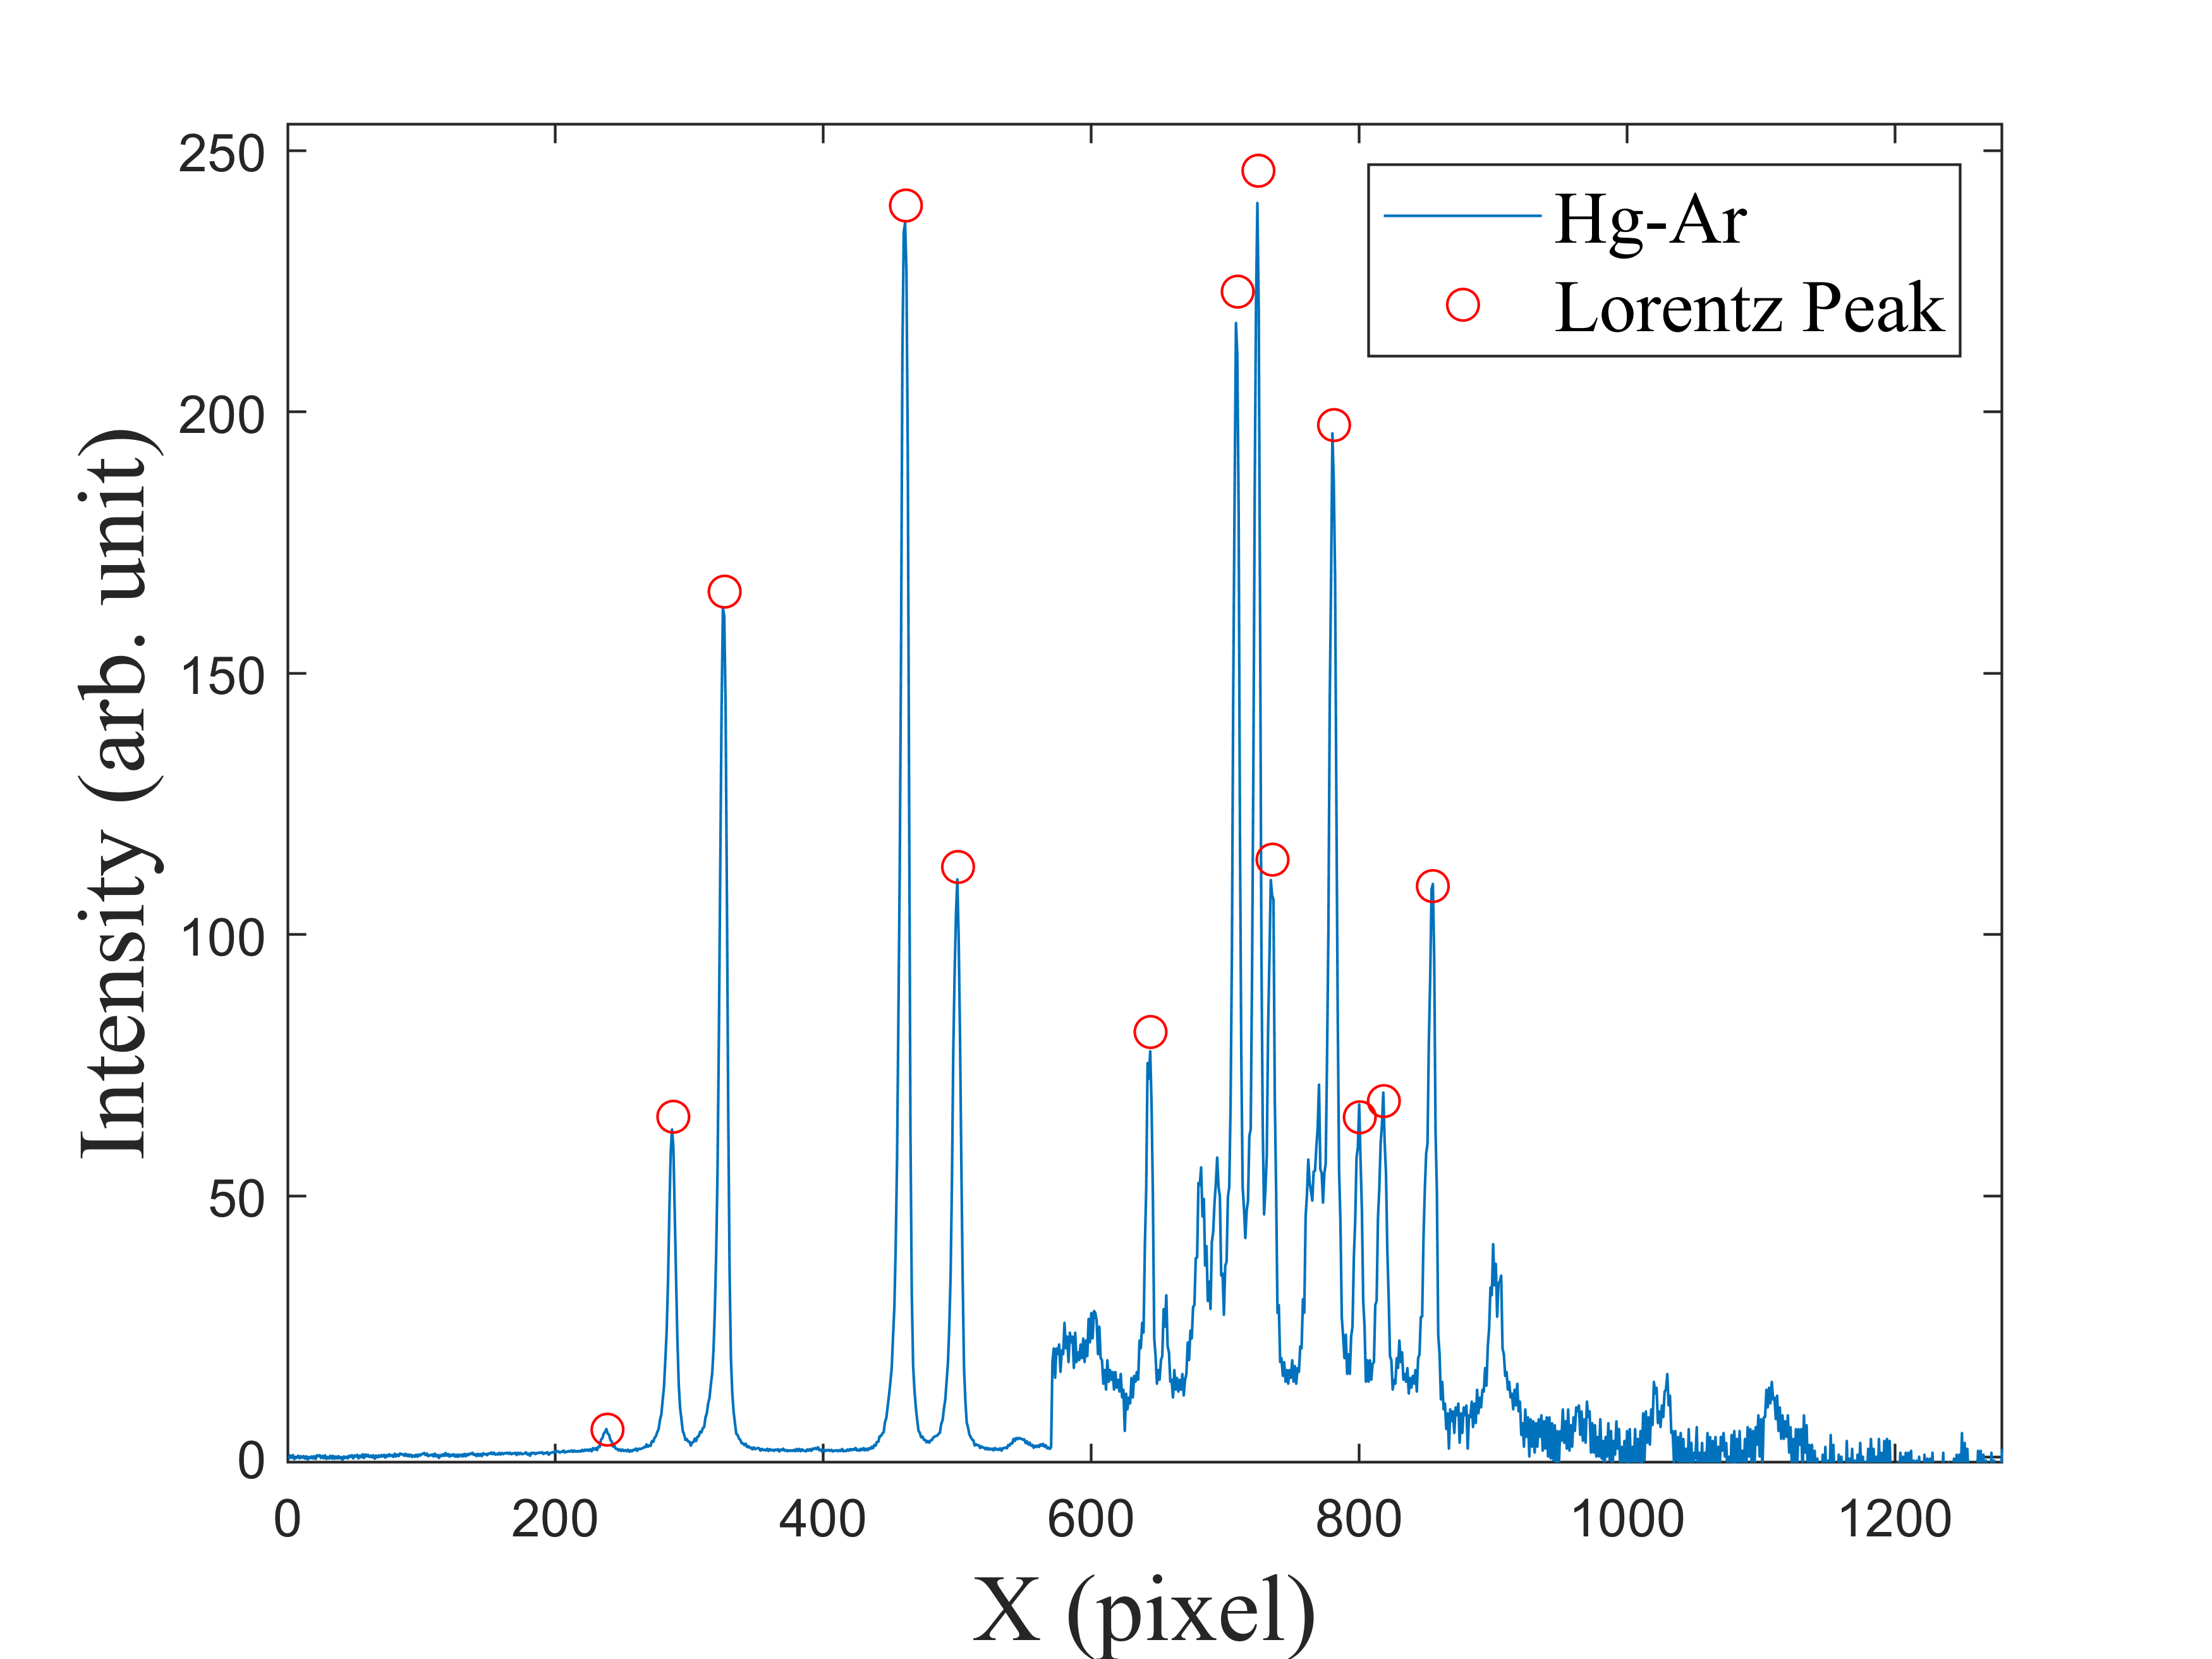
\includegraphics[width=16cm]{figures/與估測峰值比對後峰值.png} %插入图片,[]中设置图片大小,{}中是图片文件名
	\caption{區域分割後數據剔除無效峰值點後精確波峰位置結果圖} %最终文档中希望显示的图片标题
	\label{區域分割後數據剔除無效峰值點後精確波峰位置結果圖} %用于文内引用的标签
\end{figure}
在初步去除所有無效峰值點後,透過以勞倫茲模型擬合後找出的精確峰值位置與其強度及半高全寬數據如表\ref{汞氬燈高斯擬合求得參數表}. 所示。
\newpage
\begin{center}
	\vspace{0.8cm}
	\captionof{table}{汞氬燈高斯擬合求得參數表}\label{汞氬燈高斯擬合求得參數表}
\begin{tabularx}{\textwidth}{m{0.2\textwidth}<{\centering}m{0.2\textwidth}<{\centering}m{0.25\textwidth}<{\centering}m{0.2\textwidth}<{\centering}}
	\hline\hline
	光源            & 峰值位置(pixel) & 強度 & 半高全寬(pixel) \\
	\hline
	\multirow{5}{*}{汞燈 }
	&238.8276368&    5.270303917& 5.2307\\
	&287.9697699&	65.14440122& 5.7020\\
	&326.3158442&	171.58091  & 5.6381\\
	&461.6027204&	253.7391256& 5.1501\\
	&500.5412743&	112.9370475& 5.8473\\
	\hline
	\multirow{8}{*}{氬燈 }
	&644.2331809&	81.36141267& 3.8002\\
	&709.2949685&	223.0211324& 3.9613\\
	&724.7514346&	246.1550526& 3.8504\\
	&735.3158606&	114.3412062& 3.2691\\
	&781.2286706&	197.4903351& 2.9736\\
	&800.4412516&	65.04398951& 3.9324\\
	&818.4181357&	68.13802375& 4.1103\\
	&854.9459689&	109.2759383& 4.8757\\                     
	\hline\hline
\end{tabularx}
\vspace{10pt}
\end{center}
\par 
由表\ref{汞氬燈高斯擬合求得參數表}. 及圖\ref{區域分割後數據剔除無效峰值點後精確波峰位置結果圖}. 可知,雖以預測峰值位置除去多餘峰值點,但仍不全然為目標波峰,在此階段本文利用光譜波峰位置與強度雖然每次量測都不同,但峰值間彼此的距離是相同的特性。當在以相同影像感測器情況下,現已知汞燈區的最後一個波峰像素位置與氬燈兩目標波峰分別相差225個像素與280個像素,留下與此距離最接近的兩個氬燈區波峰後,最後所有目標波峰的準確波峰位置與強度如圖\ref{最終目標波峰的峰值位置與強度結果圖}. 所示,詳細資訊如表\ref{最終目標波峰參數表}. 所示,並將資訊紀錄於程式暫存記憶體中。
\begin{figure}[H] %H为当前位置,!htb为忽略美学标准,htbp为浮动图形
	\centering %图片居中
	%\setlength{\abovecaptionskip}{1cm}
	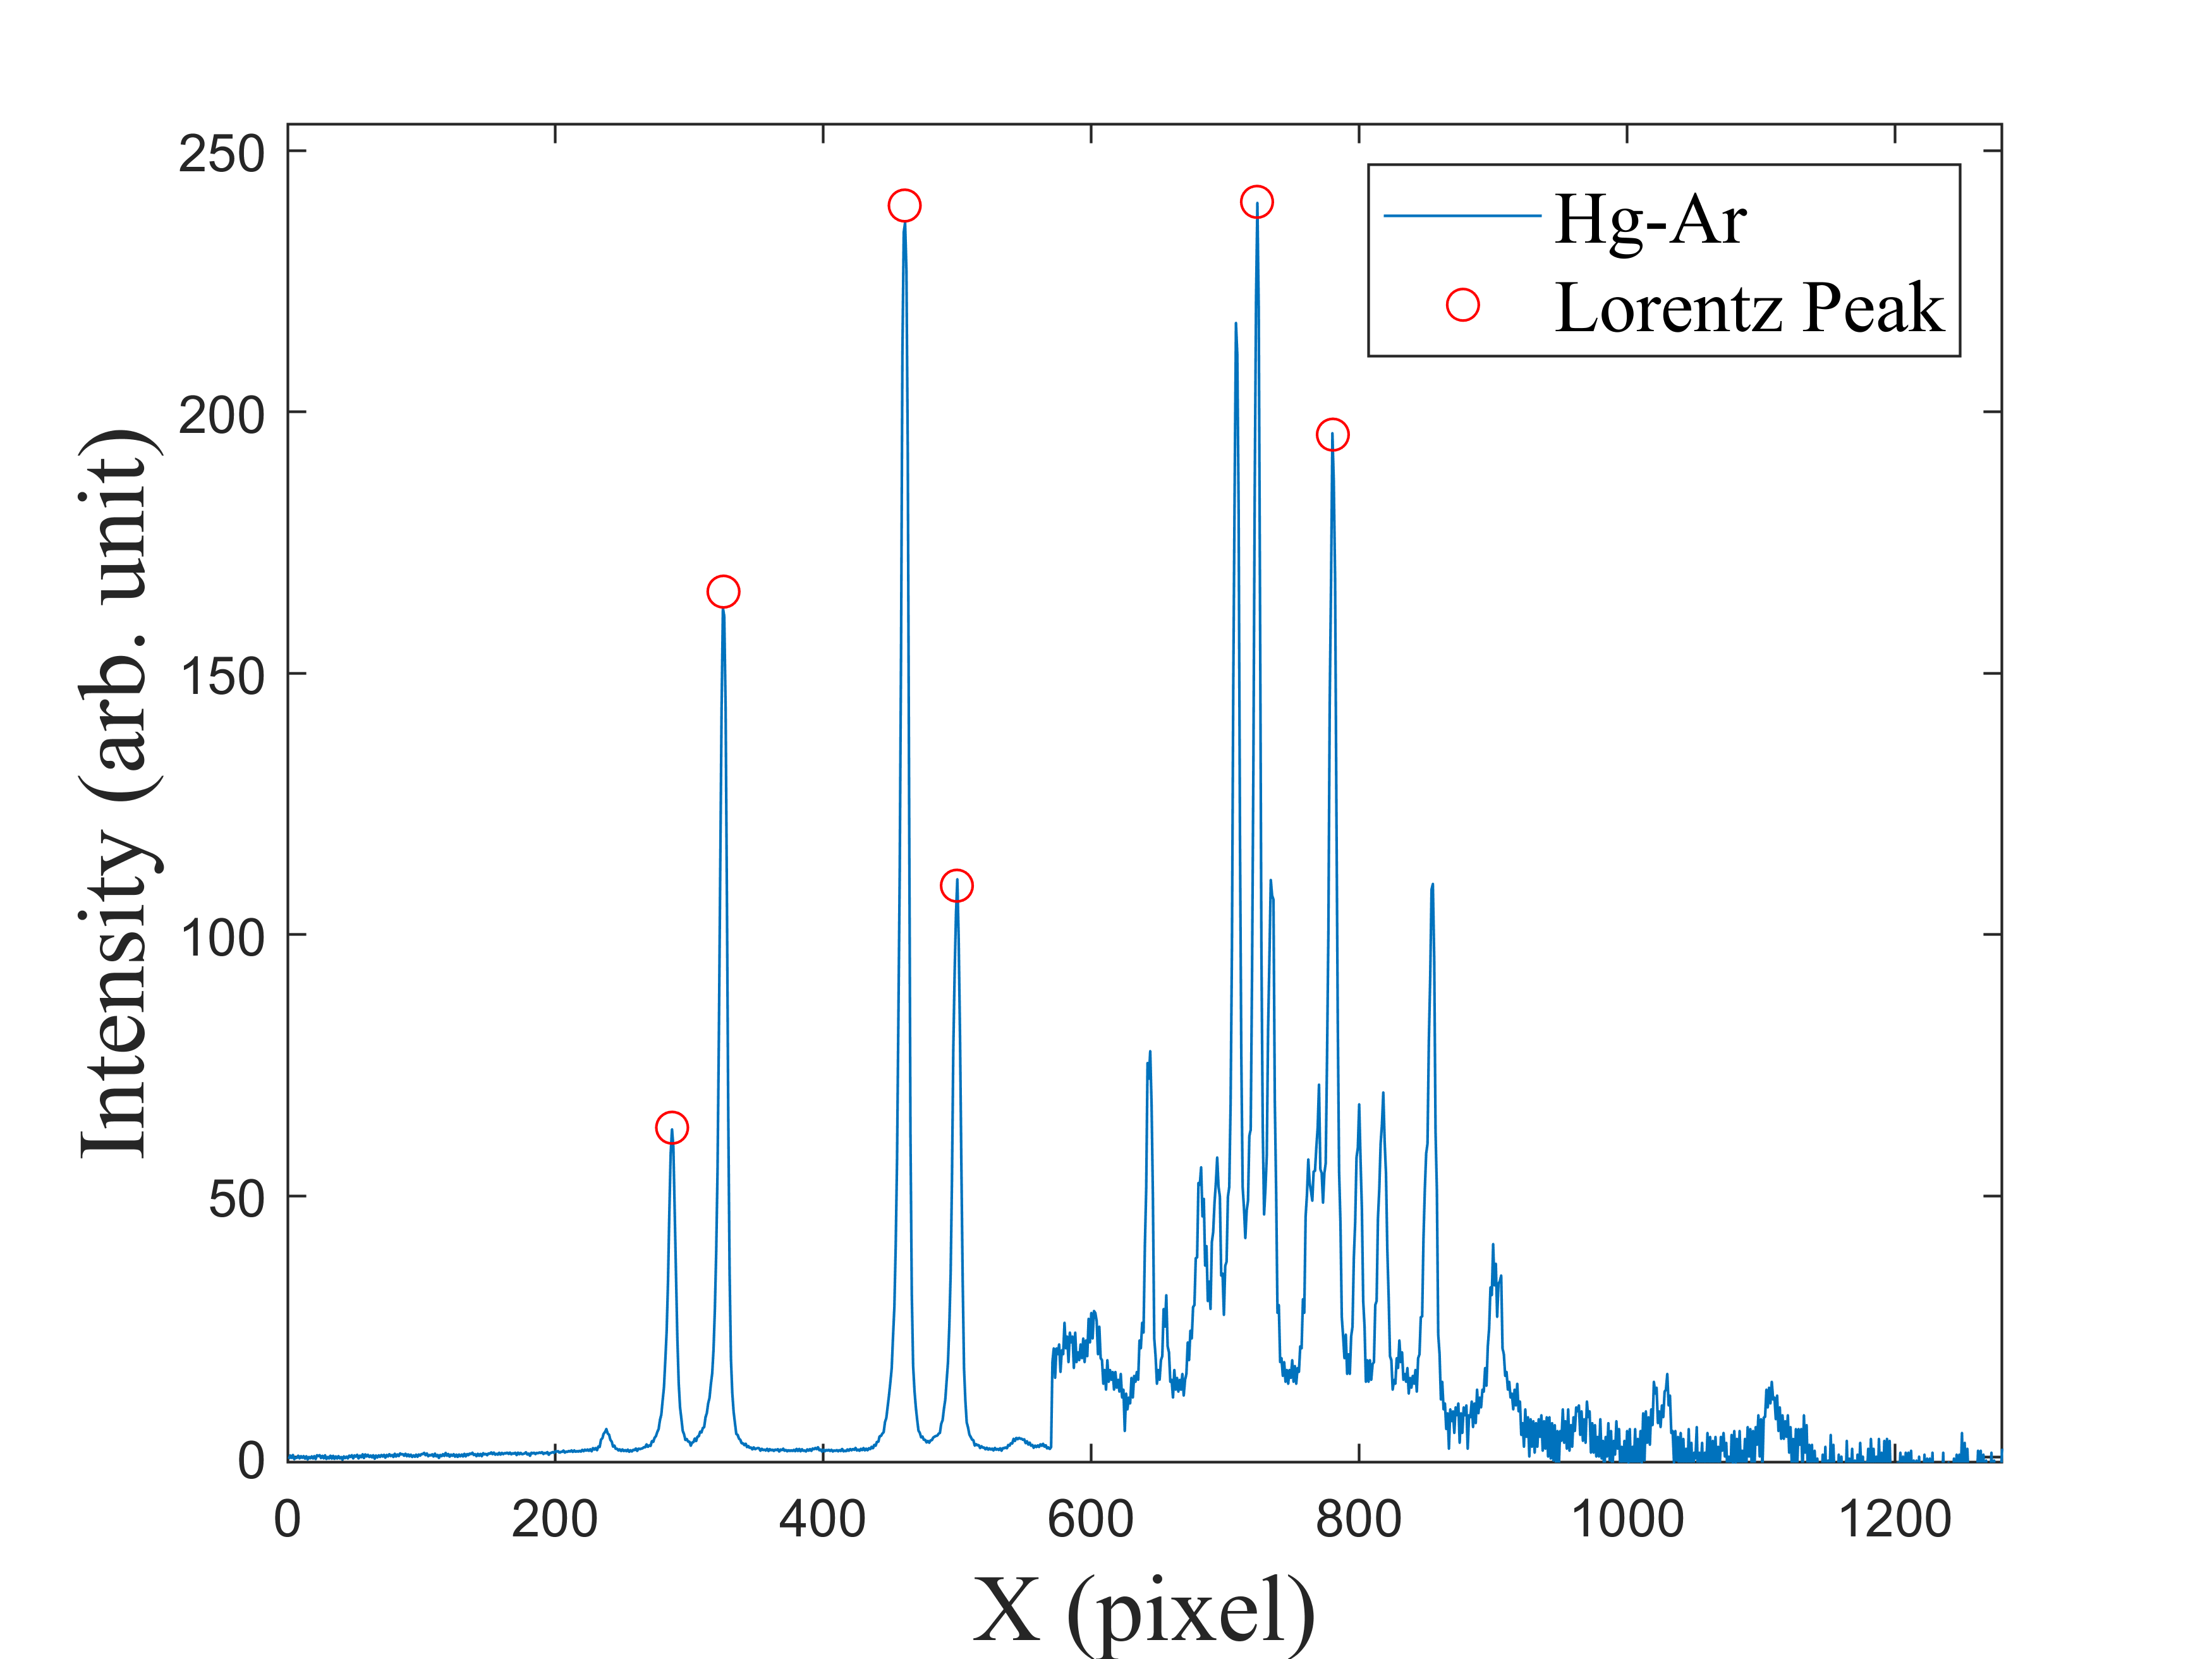
\includegraphics[width=16cm]{figures/comebine_hg_ar_最終PEAK.png} %插入图片,[]中设置图片大小,{}中是图片文件名
	\caption{最終目標波峰的峰值位置與強度結果圖} %最终文档中希望显示的图片标题
	\label{最終目標波峰的峰值位置與強度結果圖} %用于文内引用的标签
\end{figure}

\begin{center}
\vspace{0.8cm}
\captionof{table}{最終目標波峰參數表}\label{最終目標波峰參數表}
\begin{tabularx}{\textwidth}{m{0.2\textwidth}<{\centering} m{0.21\textwidth}<{\centering} m{0.25\textwidth}<{\centering}c}
	\hline\hline
	光源            & 峰值位置(pixel) & 強度 & 半高全寬(pixel) \\
	\hline
    \multirow{4}{*}{汞燈 }
    &287.9697699&	65.14440122& 5.7020\\
    &326.3158442&	171.58091  & 5.6381\\
    &461.6027204&	253.7391256& 5.1501\\
    &500.5412743&	112.9370475& 5.8473\\
    \hline
    \multirow{2}{*}{氬燈 }
    &724.7514346&	246.1550526& 3.8504\\
    &781.2286706&	197.4903351& 2.9736\\                   
	\hline\hline
\end{tabularx}
\end{center}
\subsection{單雷射波峰位置偵測}
相對於汞氬燈源來說,雷射光源十分的不穩定,燈源跳動造成AutoScaling完成後的光源無法穩定在同一強度上,使得無法精確取到強度為AutoScaling完成時的數據,所幸雷射光源波型單調,波峰僅有雷射光源與其二階光\cite{diffraction-2nd-Light}此二波峰,且兩者強度相差極大,因此透過強度閥值便可以過濾掉二階光產生的波峰。\par
當一雷射光源輸入且已經由AutoScaling調整至適當強度後,波型如圖\ref{雷射光譜強度波型圖}. 所示,雷射波形於表\ref{光源介紹表}. 說明,其特定波長能量放大所產生之光束,能以勞倫茲模型擬合逼近,因此在進行雷射波峰位置偵測時,將採用勞倫茲擬合來找出準確波峰位置、半高全寬與強度值。
\begin{figure}[H] %H为当前位置,!htb为忽略美学标准,htbp为浮动图形
	\centering %图片居中
	\vspace{0.8cm}
	%\setlength{\abovecaptionskip}{1cm}
	\setlength{\abovecaptionskip}{0.cm}
	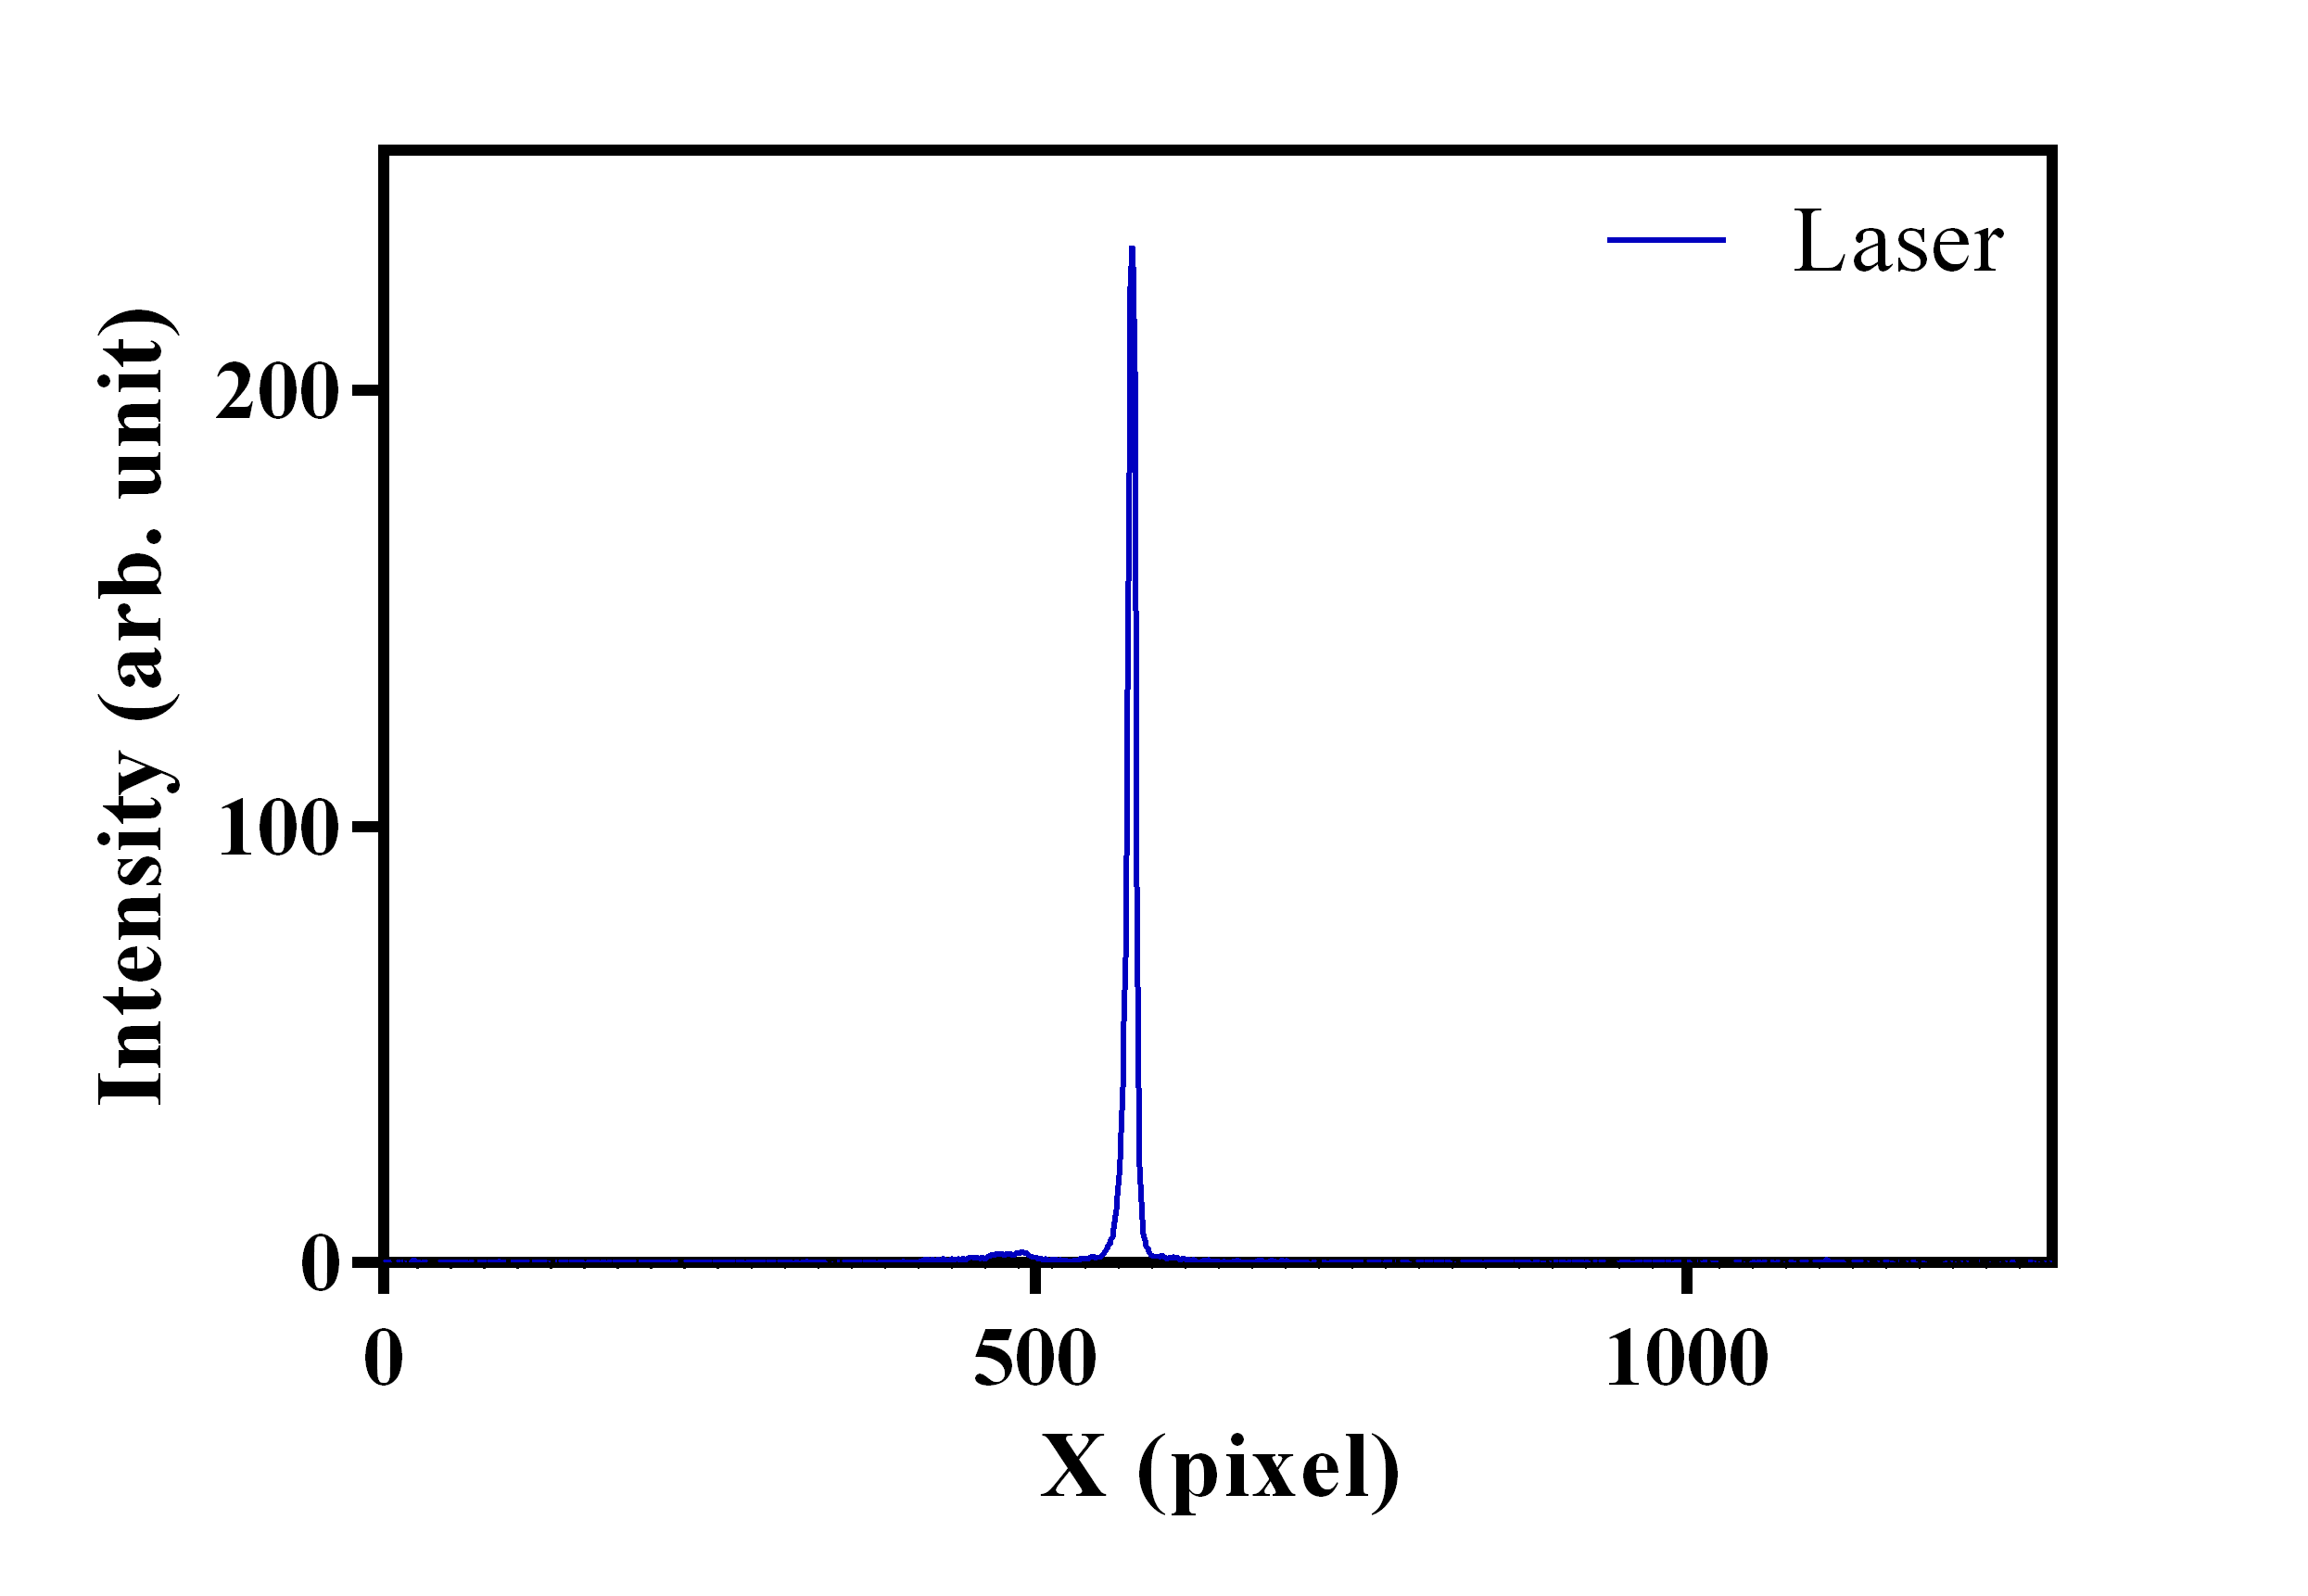
\includegraphics[width=\textwidth]{figures/Laser_raw.png} %插入图片,[]中设置图片大小,{}中是图片文件名
	\caption{雷射光譜強度波型圖} %最终文档中希望显示的图片标题
	\label{雷射光譜強度波型圖} %用于文内引用的标签
\end{figure}
由圖\ref{雷射光譜強度波型圖}. 中可看出此雷射之二階光位置落於影像感測器外,但考量到波長較短的雷射所產生二階光如圖\ref{較短波長的雷射光譜強度波型圖}. 所示,仍會落在影像感測器中,因此在光譜波形套用勞倫茲模型擬合前,仍需對數據進行分區,確保所有分割後區域內僅存在一波峰。
\begin{figure}[H] %H为当前位置,!htb为忽略美学标准,htbp为浮动图形
	\centering %图片居中
	\vspace{0.8cm}
	%\setlength{\abovecaptionskip}{1cm}
	\setlength{\abovecaptionskip}{0.cm}
	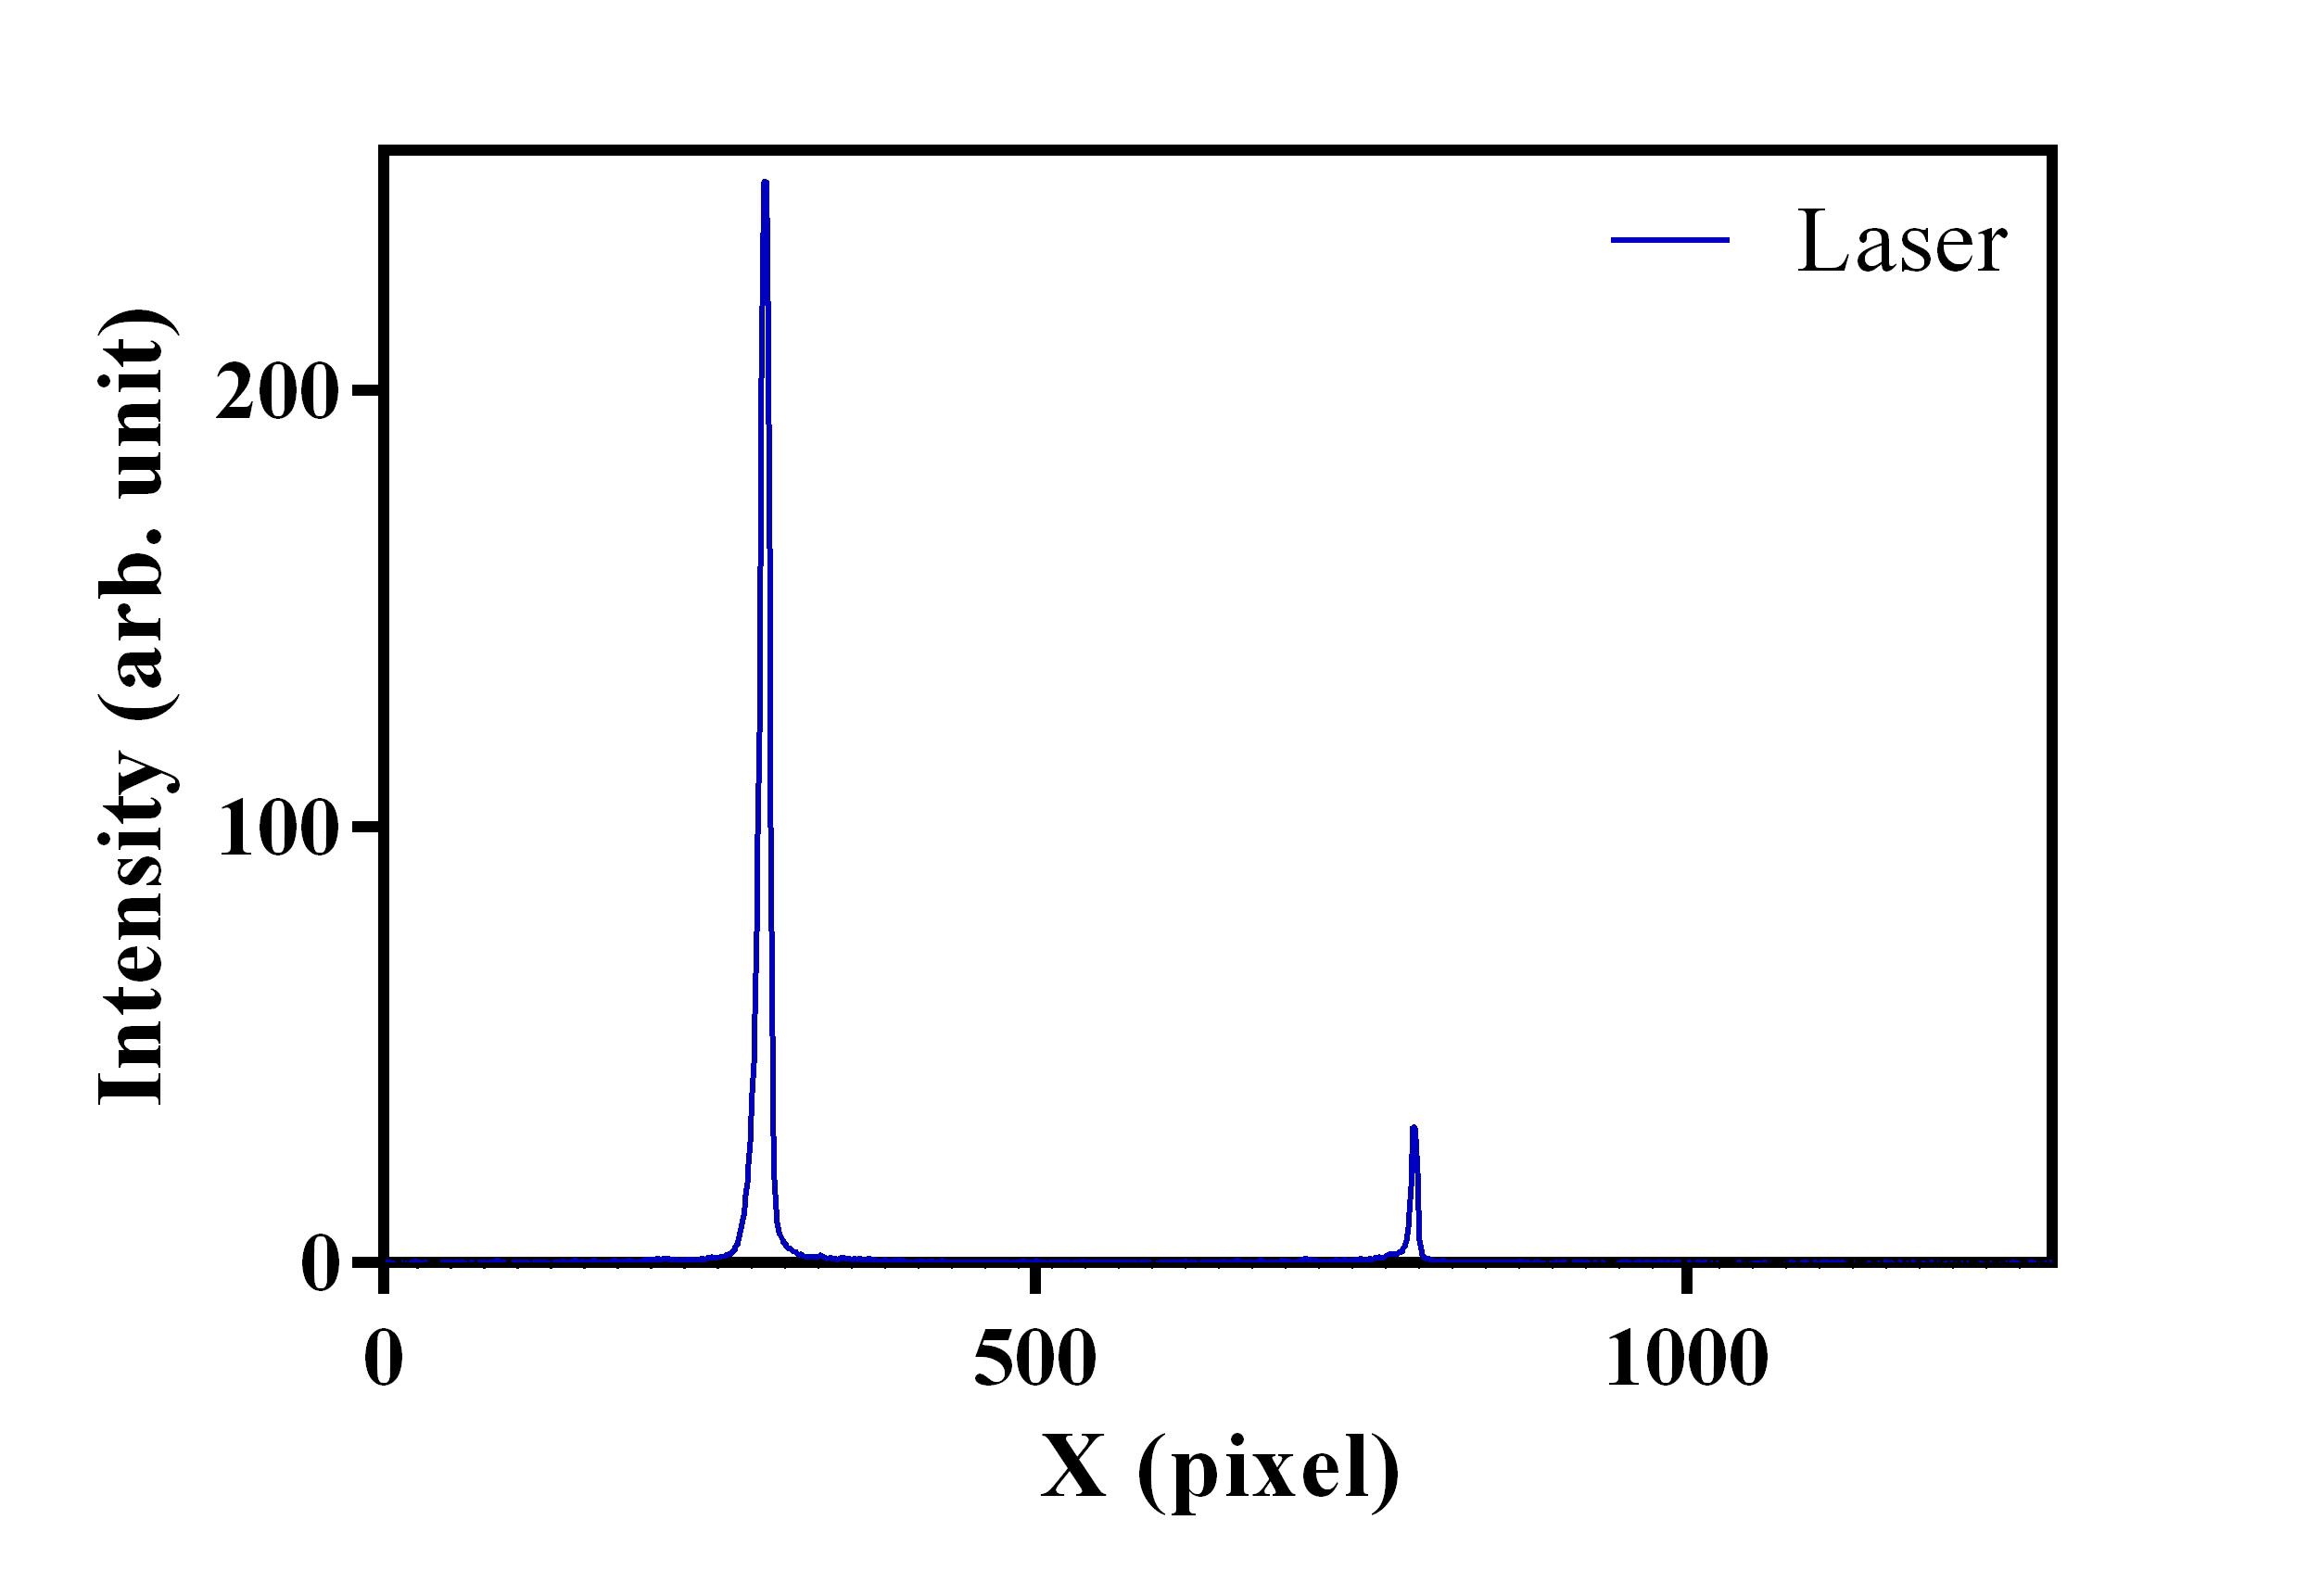
\includegraphics[width=\textwidth]{figures/Laser_1.png} %插入图片,[]中设置图片大小,{}中是图片文件名
	\caption{較短波長的雷射光譜強度波型圖} %最终文档中希望显示的图片标题
	\label{較短波長的雷射光譜強度波型圖} %用于文内引用的标签
\end{figure}
雷射區域分割的判定方法與汞氬燈相同,使用斜率分割出波峰所在區域,再以強度過濾二階光的波峰區域。首先找出所有雷射光譜數據的區域最大與最小值,並將所有點數依像素位置猶大至小排列,如圖\ref{雷射光譜區域最大值與最小值像素位置表示圖}. 所示。波峰所在位置必定為一區域最大值,且此一區域最大值不同於其餘區域最大值,斜率必將夾於一正斜率線段與負斜率線段中,且此一斜率絕對值將遠高於其餘線段斜率,因此透過兩點間斜率判定與斜率正負夾擠法,便可以過濾出如圖\ref{雷射光譜以斜率分割後之波峰區域表示圖}. 所示四點區分出兩個峰值所在區域。
\begin{figure}[H] %H为当前位置,!htb为忽略美学标准,htbp为浮动图形
	\centering %图片居中
	%\setlength{\abovecaptionskip}{1cm}
	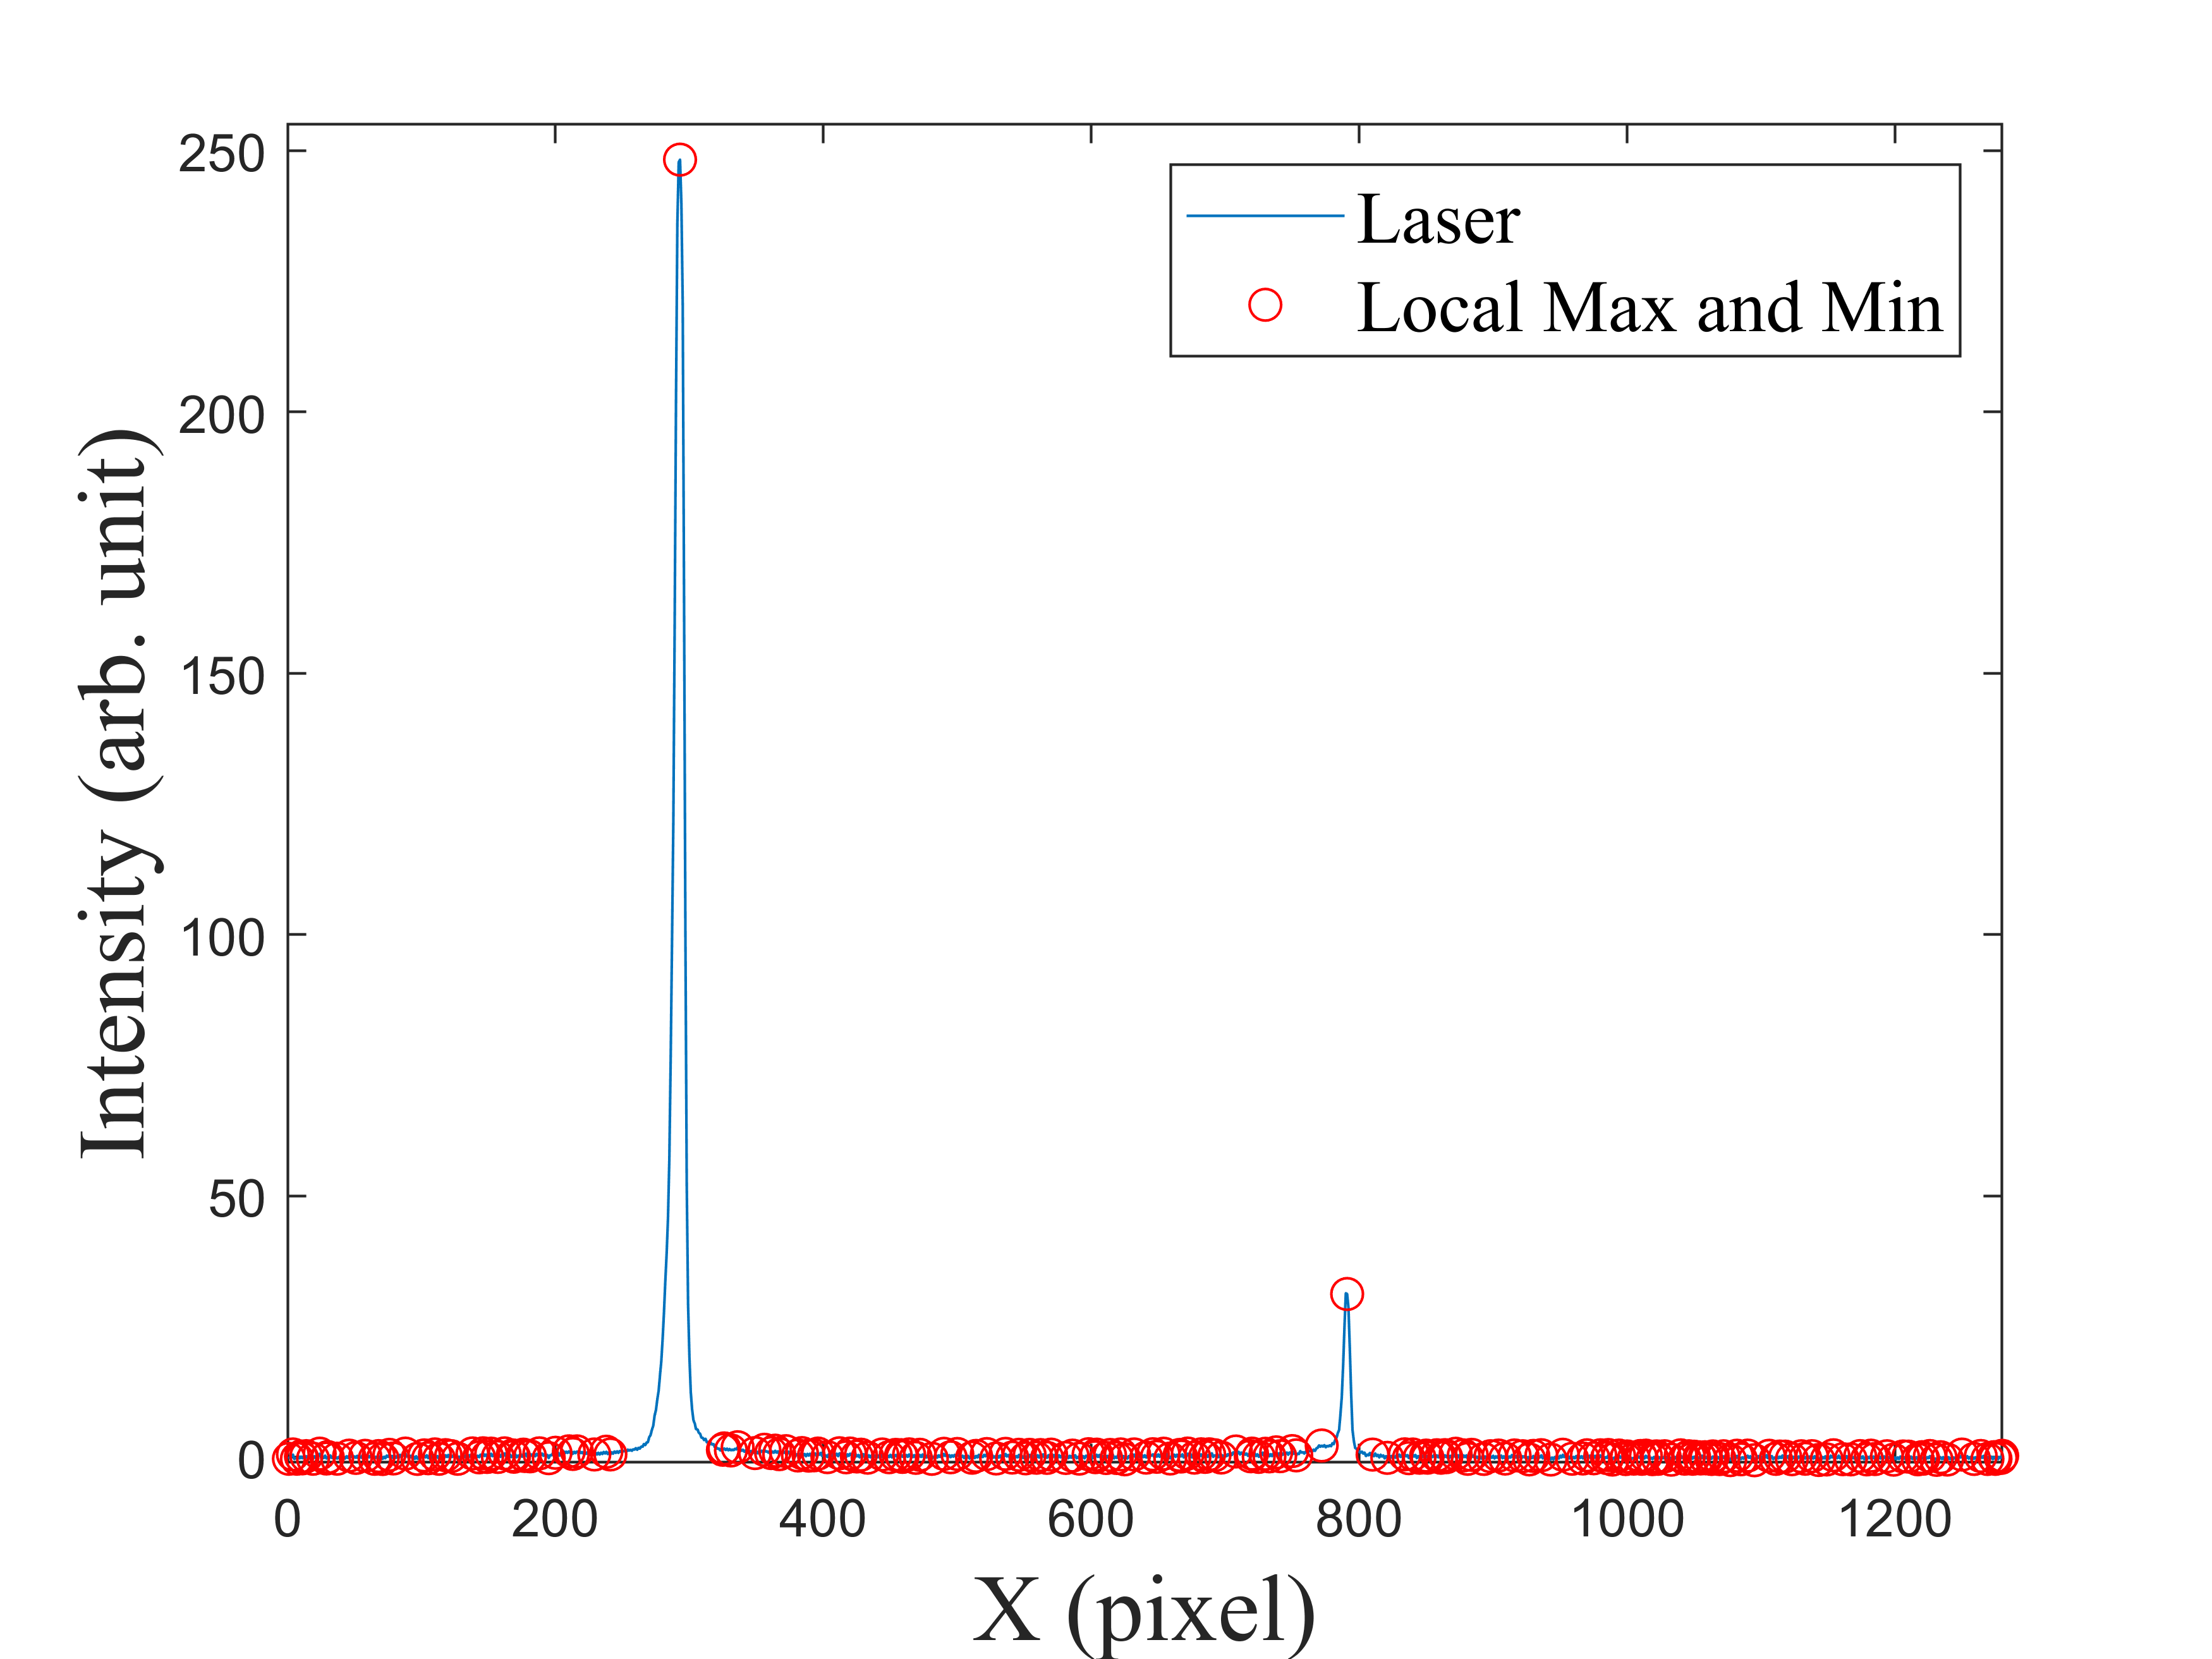
\includegraphics[width=14.5cm]{figures/LASER_MIN_MAX.png} %插入图片,[]中设置图片大小,{}中是图片文件名
	\caption{雷射光譜區域最大值與最小值像素位置表示圖} %最终文档中希望显示的图片标题
	\label{雷射光譜區域最大值與最小值像素位置表示圖} %用于文内引用的标签
\end{figure}

\begin{figure}[H] %H为当前位置,!htb为忽略美学标准,htbp为浮动图形
	\centering %图片居中
	%\setlength{\abovecaptionskip}{1cm}
	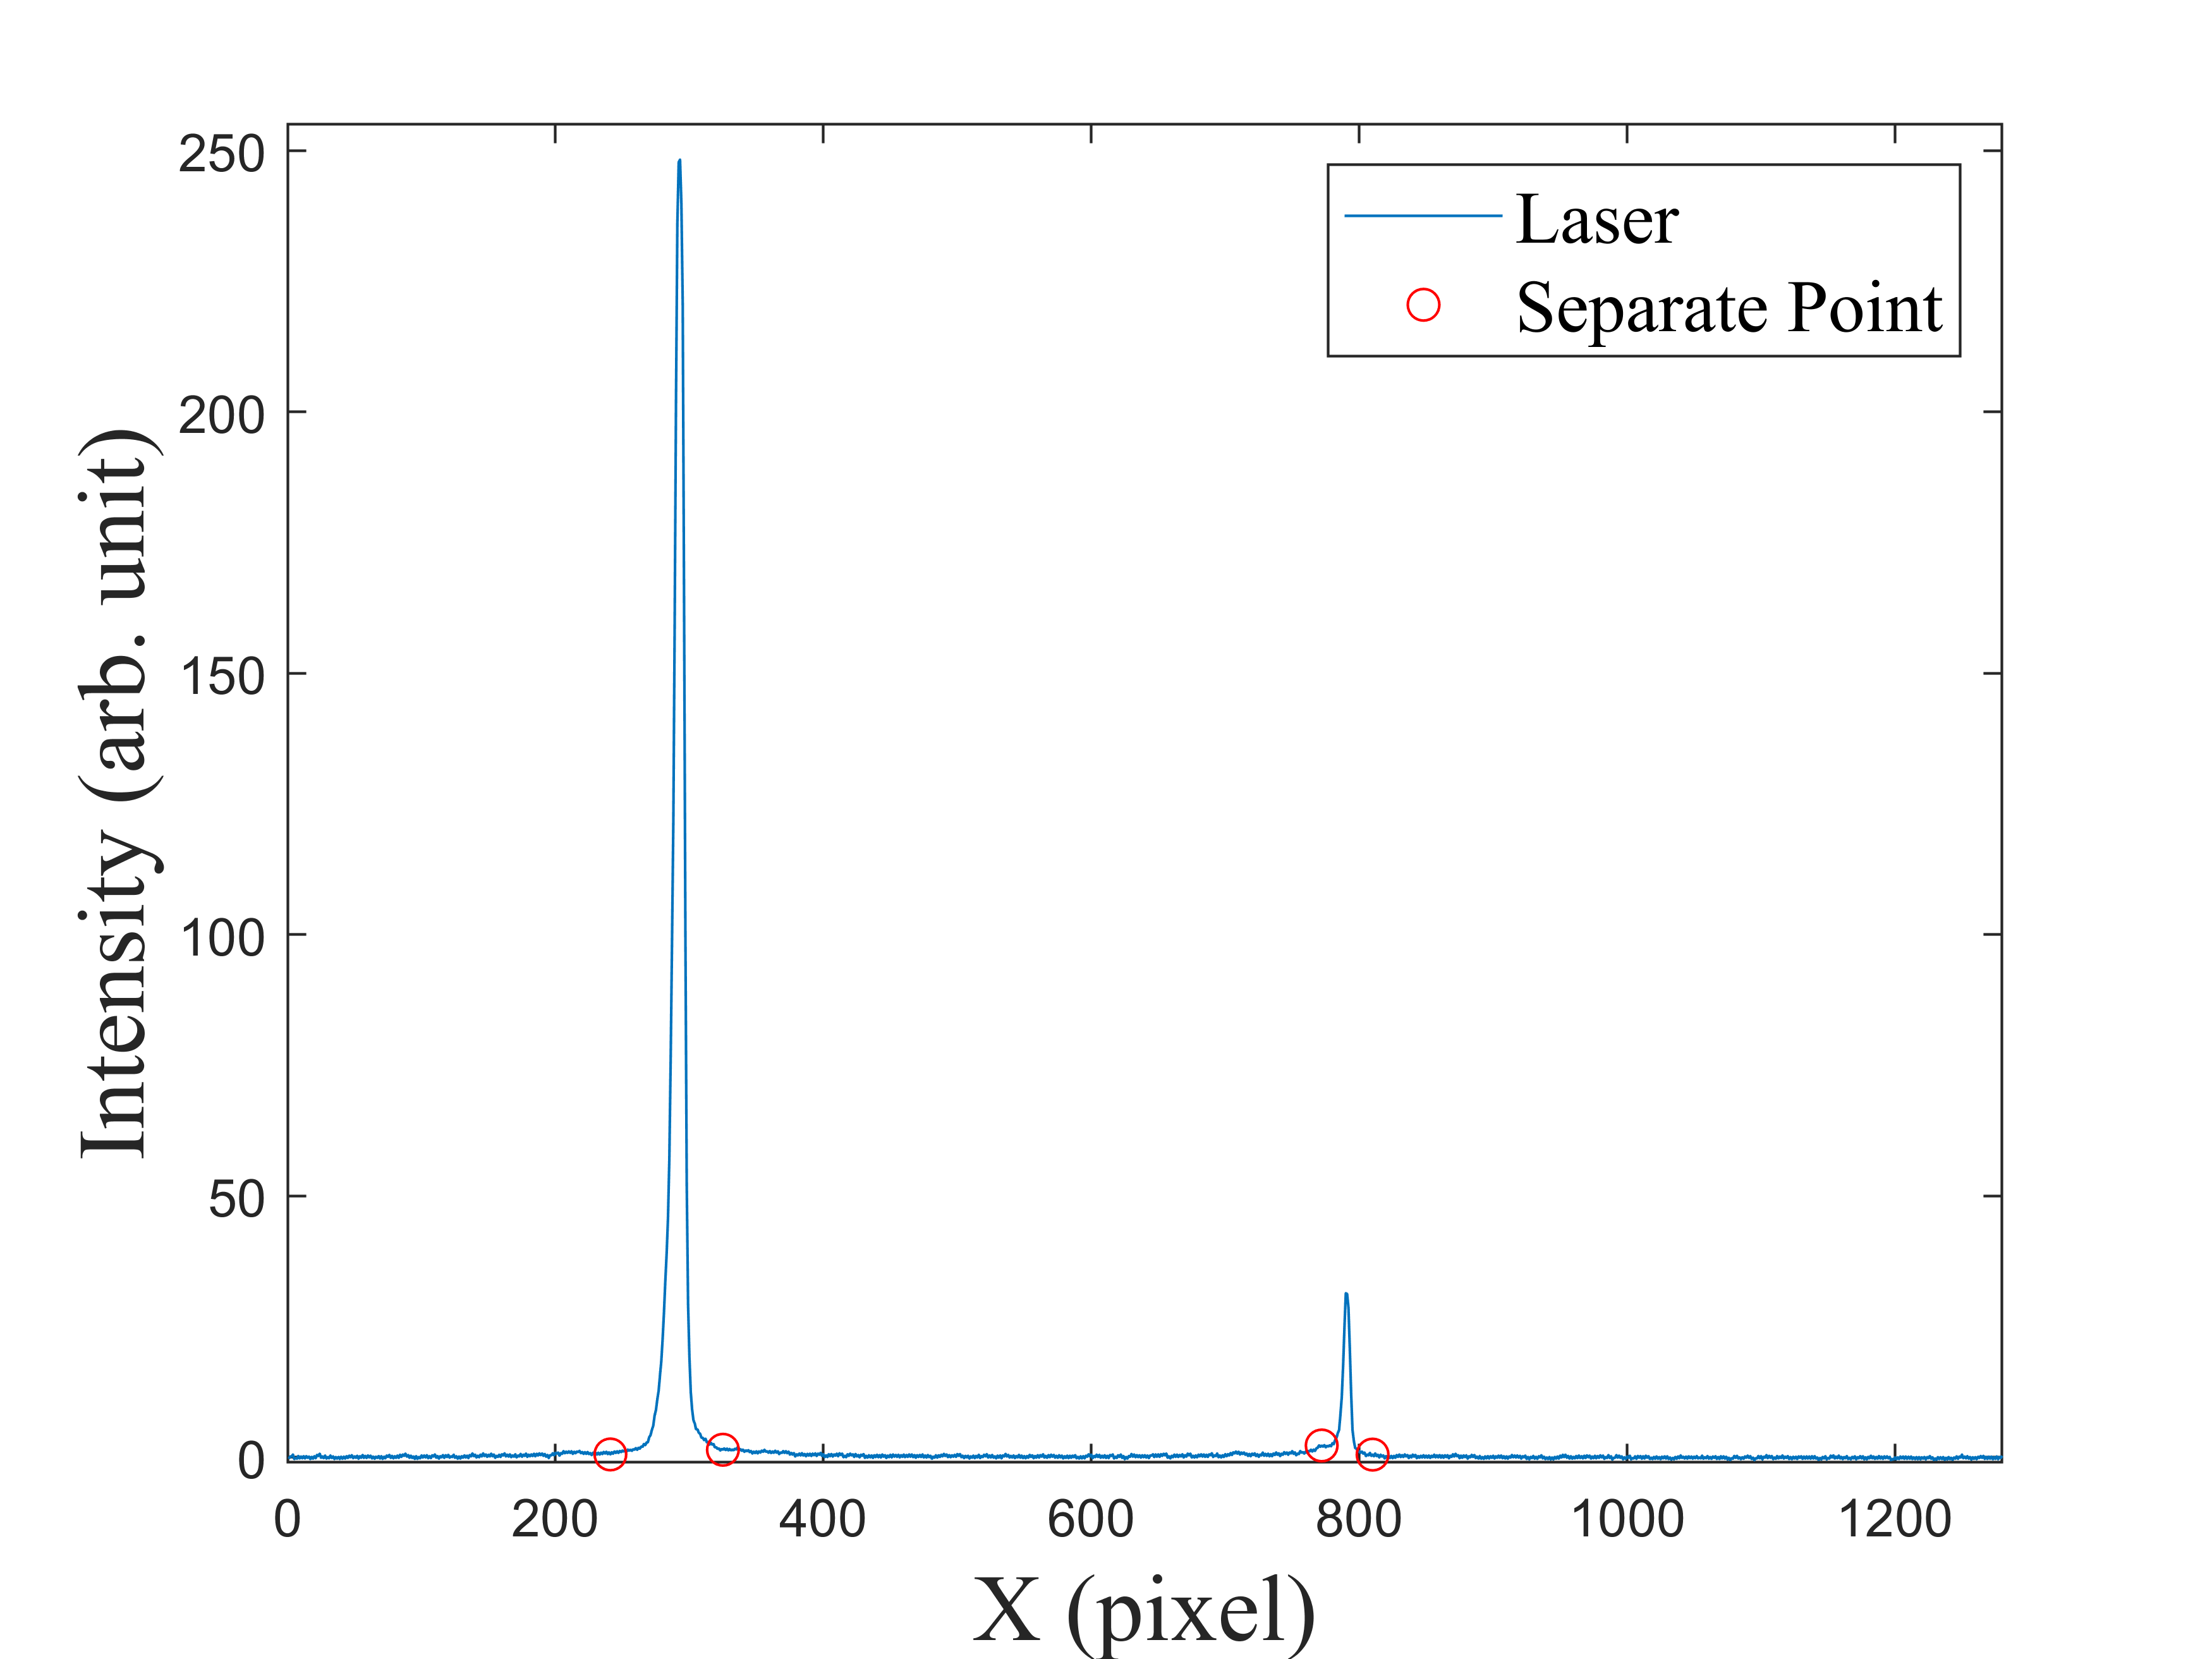
\includegraphics[width=14.5cm]{figures/LASER_SEP.png} %插入图片,[]中设置图片大小,{}中是图片文件名
	\caption{雷射光譜以斜率分割後之波峰區域表示圖} %最终文档中希望显示的图片标题
	\label{雷射光譜以斜率分割後之波峰區域表示圖} %用于文内引用的标签
\end{figure}
由圖\ref{雷射光譜以斜率分割後之波峰區域表示圖}. 中可以明顯看出,當在波長較低之雷射進行區域分割後,由於存在雷射的二階光的影響,因此數據分割後的波峰區域仍包含二階光波峰所在區域,為了要找出主要波峰的數據區域,僅需透過區域最大值的強度與其所在的位置,則可以輕易判斷出主要雷射波峰所在的區域,保留主要波峰區域並且剃除二階光產生的波峰的區域後,最後的分區結果如圖\ref{雷射光譜以強度過濾後之主波峰區域表示圖}. 所示。
\begin{figure}[H] %H为当前位置,!htb为忽略美学标准,htbp为浮动图形
	\centering %图片居中
	\vspace{0.8cm}
	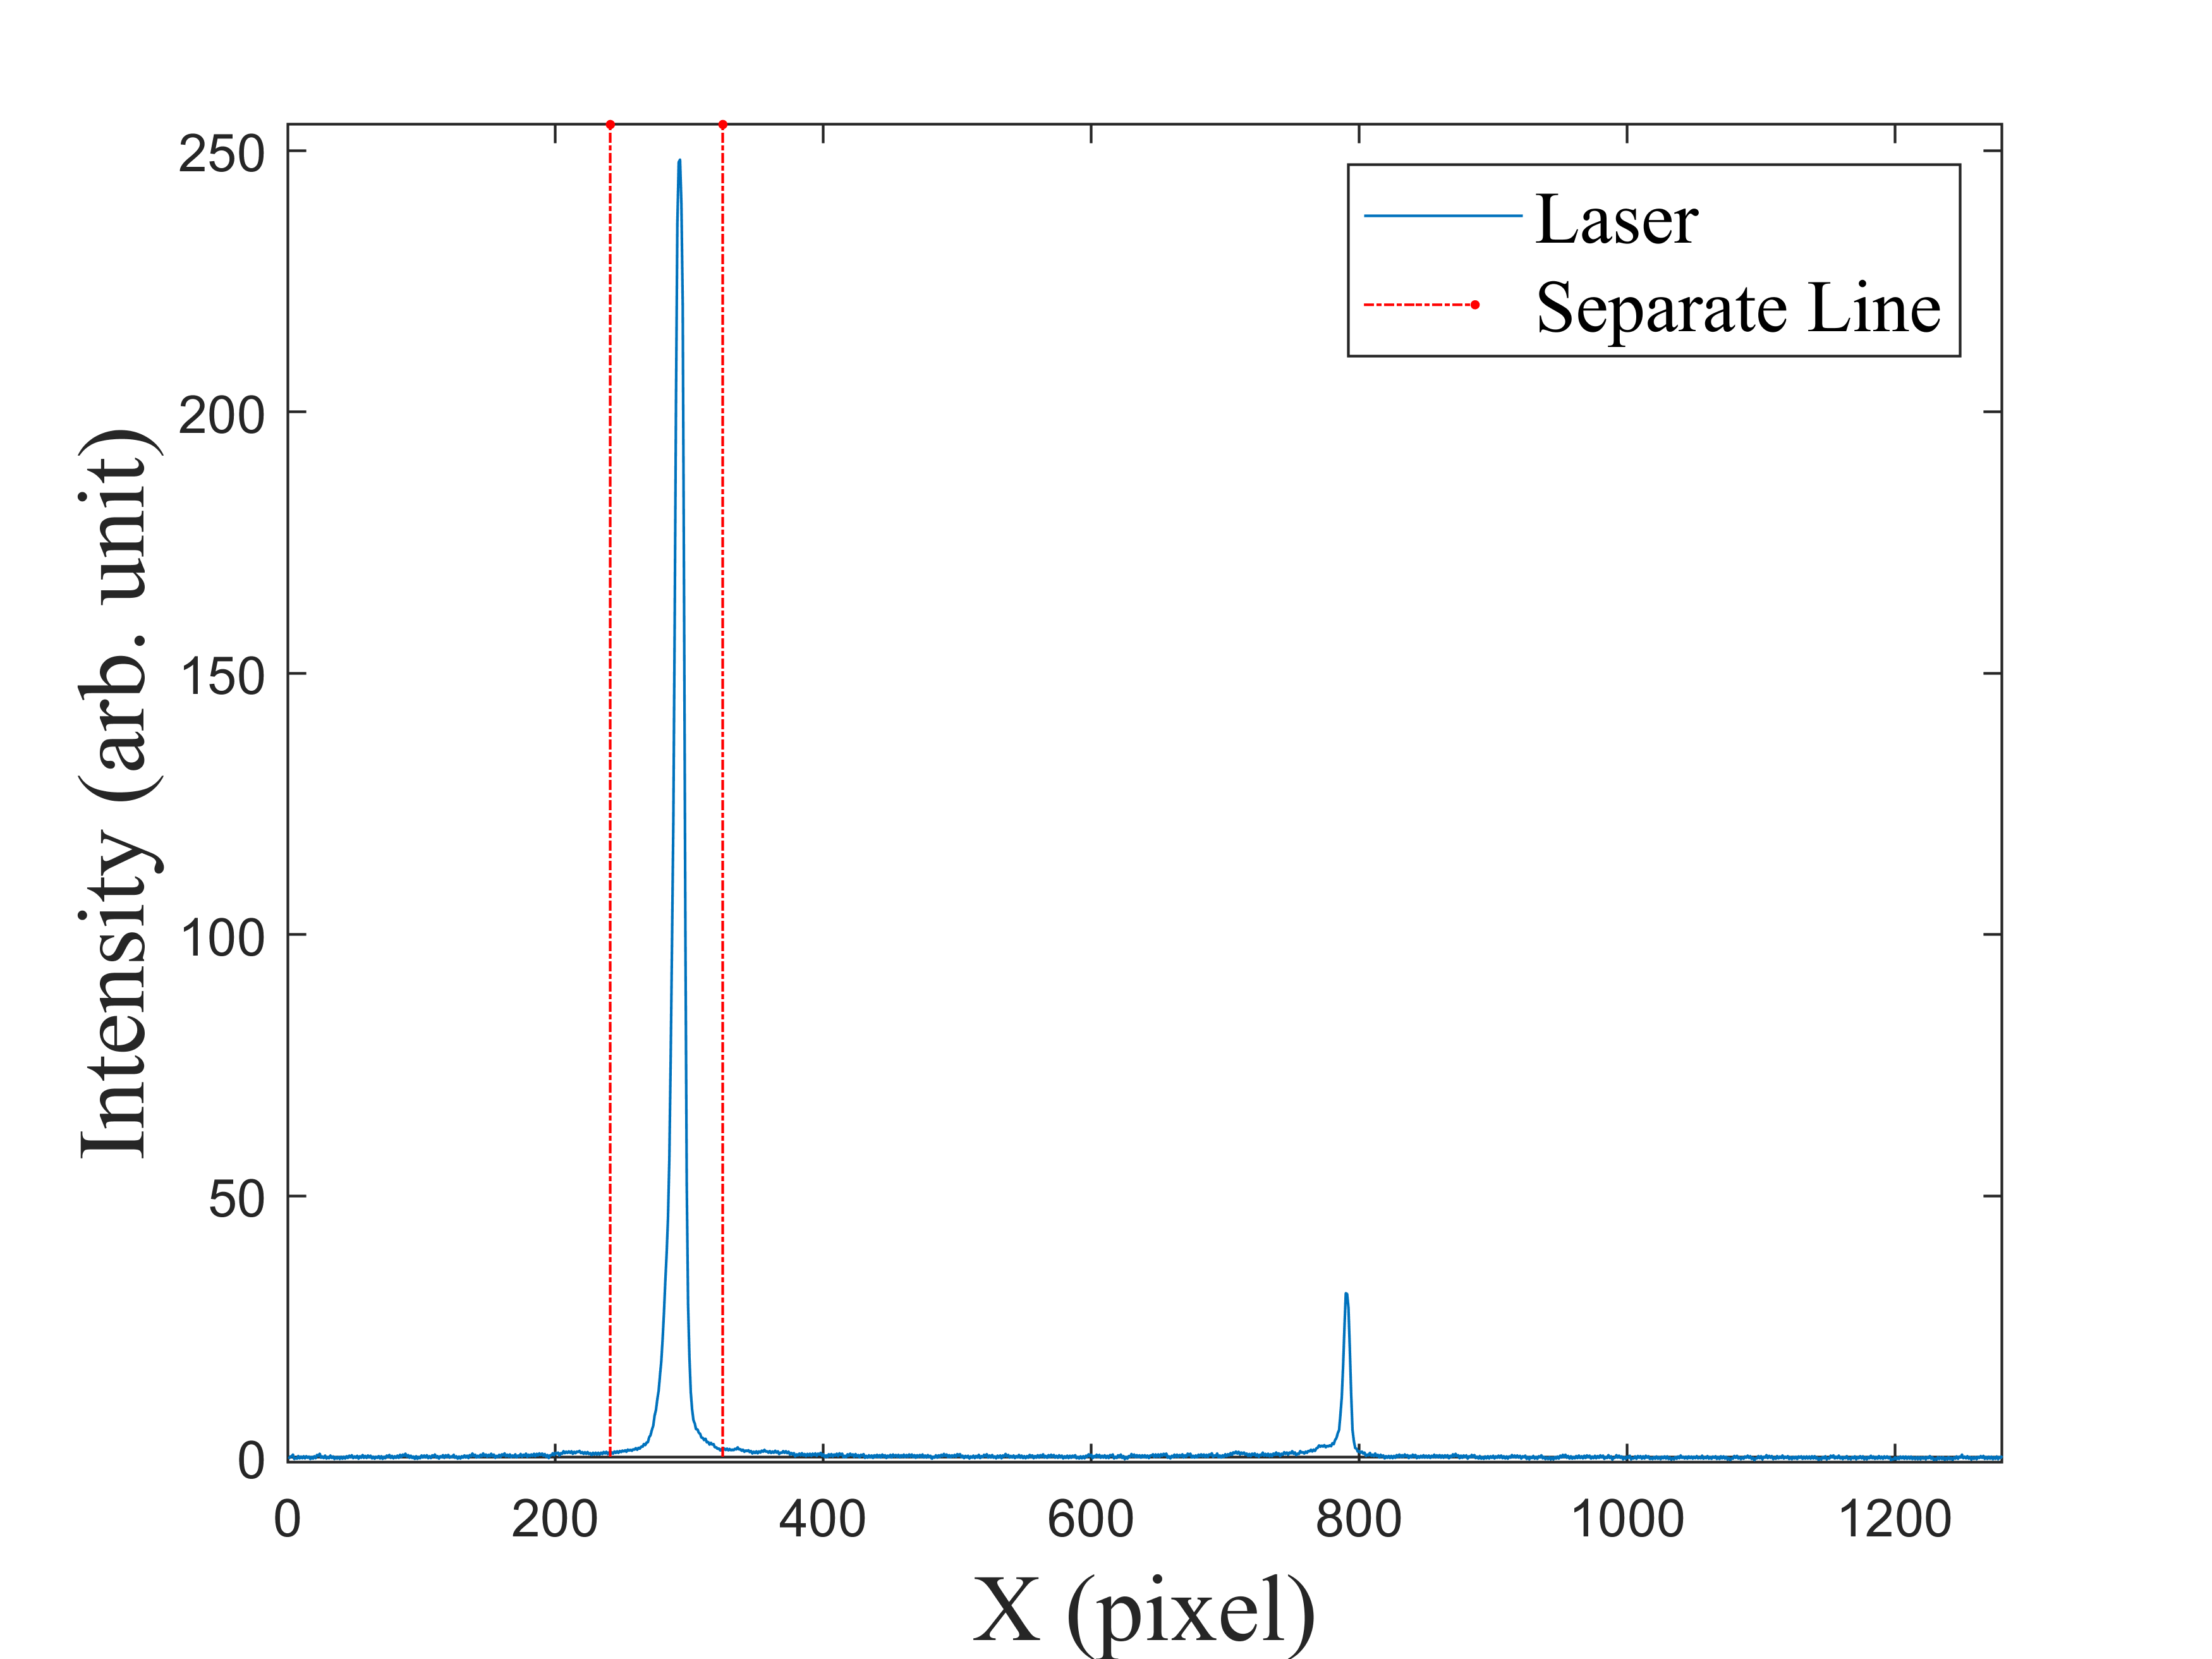
\includegraphics[width=16cm]{figures/laser_sep_only1area.png} %插入图片,[]中设置图片大小,{}中是图片文件名
	\caption{雷射光譜以強度過濾後之主波峰區域表示圖} %最终文档中希望显示的图片标题
	\label{雷射光譜以強度過濾後之主波峰區域表示圖} %用于文内引用的标签
\end{figure}
\newpage
如第二章表\ref{光源介紹表}. 所述,雷射光束的光譜波形最適合以勞倫茲模型函數擬合,因此將雷射主波峰所在區域波形數據以勞倫茲模型擬合後,便可得出雷射精確的波峰位置、半高全寬與波峰強度,擬合結果如圖\ref{雷射光譜主波峰區域進行勞倫茲擬合後結果圖}. 所示。
\begin{figure}[H] %H为当前位置,!htb为忽略美学标准,htbp为浮动图形
	\centering %图片居中
	\vspace{0.8cm}
	\setlength{\abovecaptionskip}{0.cm}
	%\setlength{\abovecaptionskip}{1cm}
	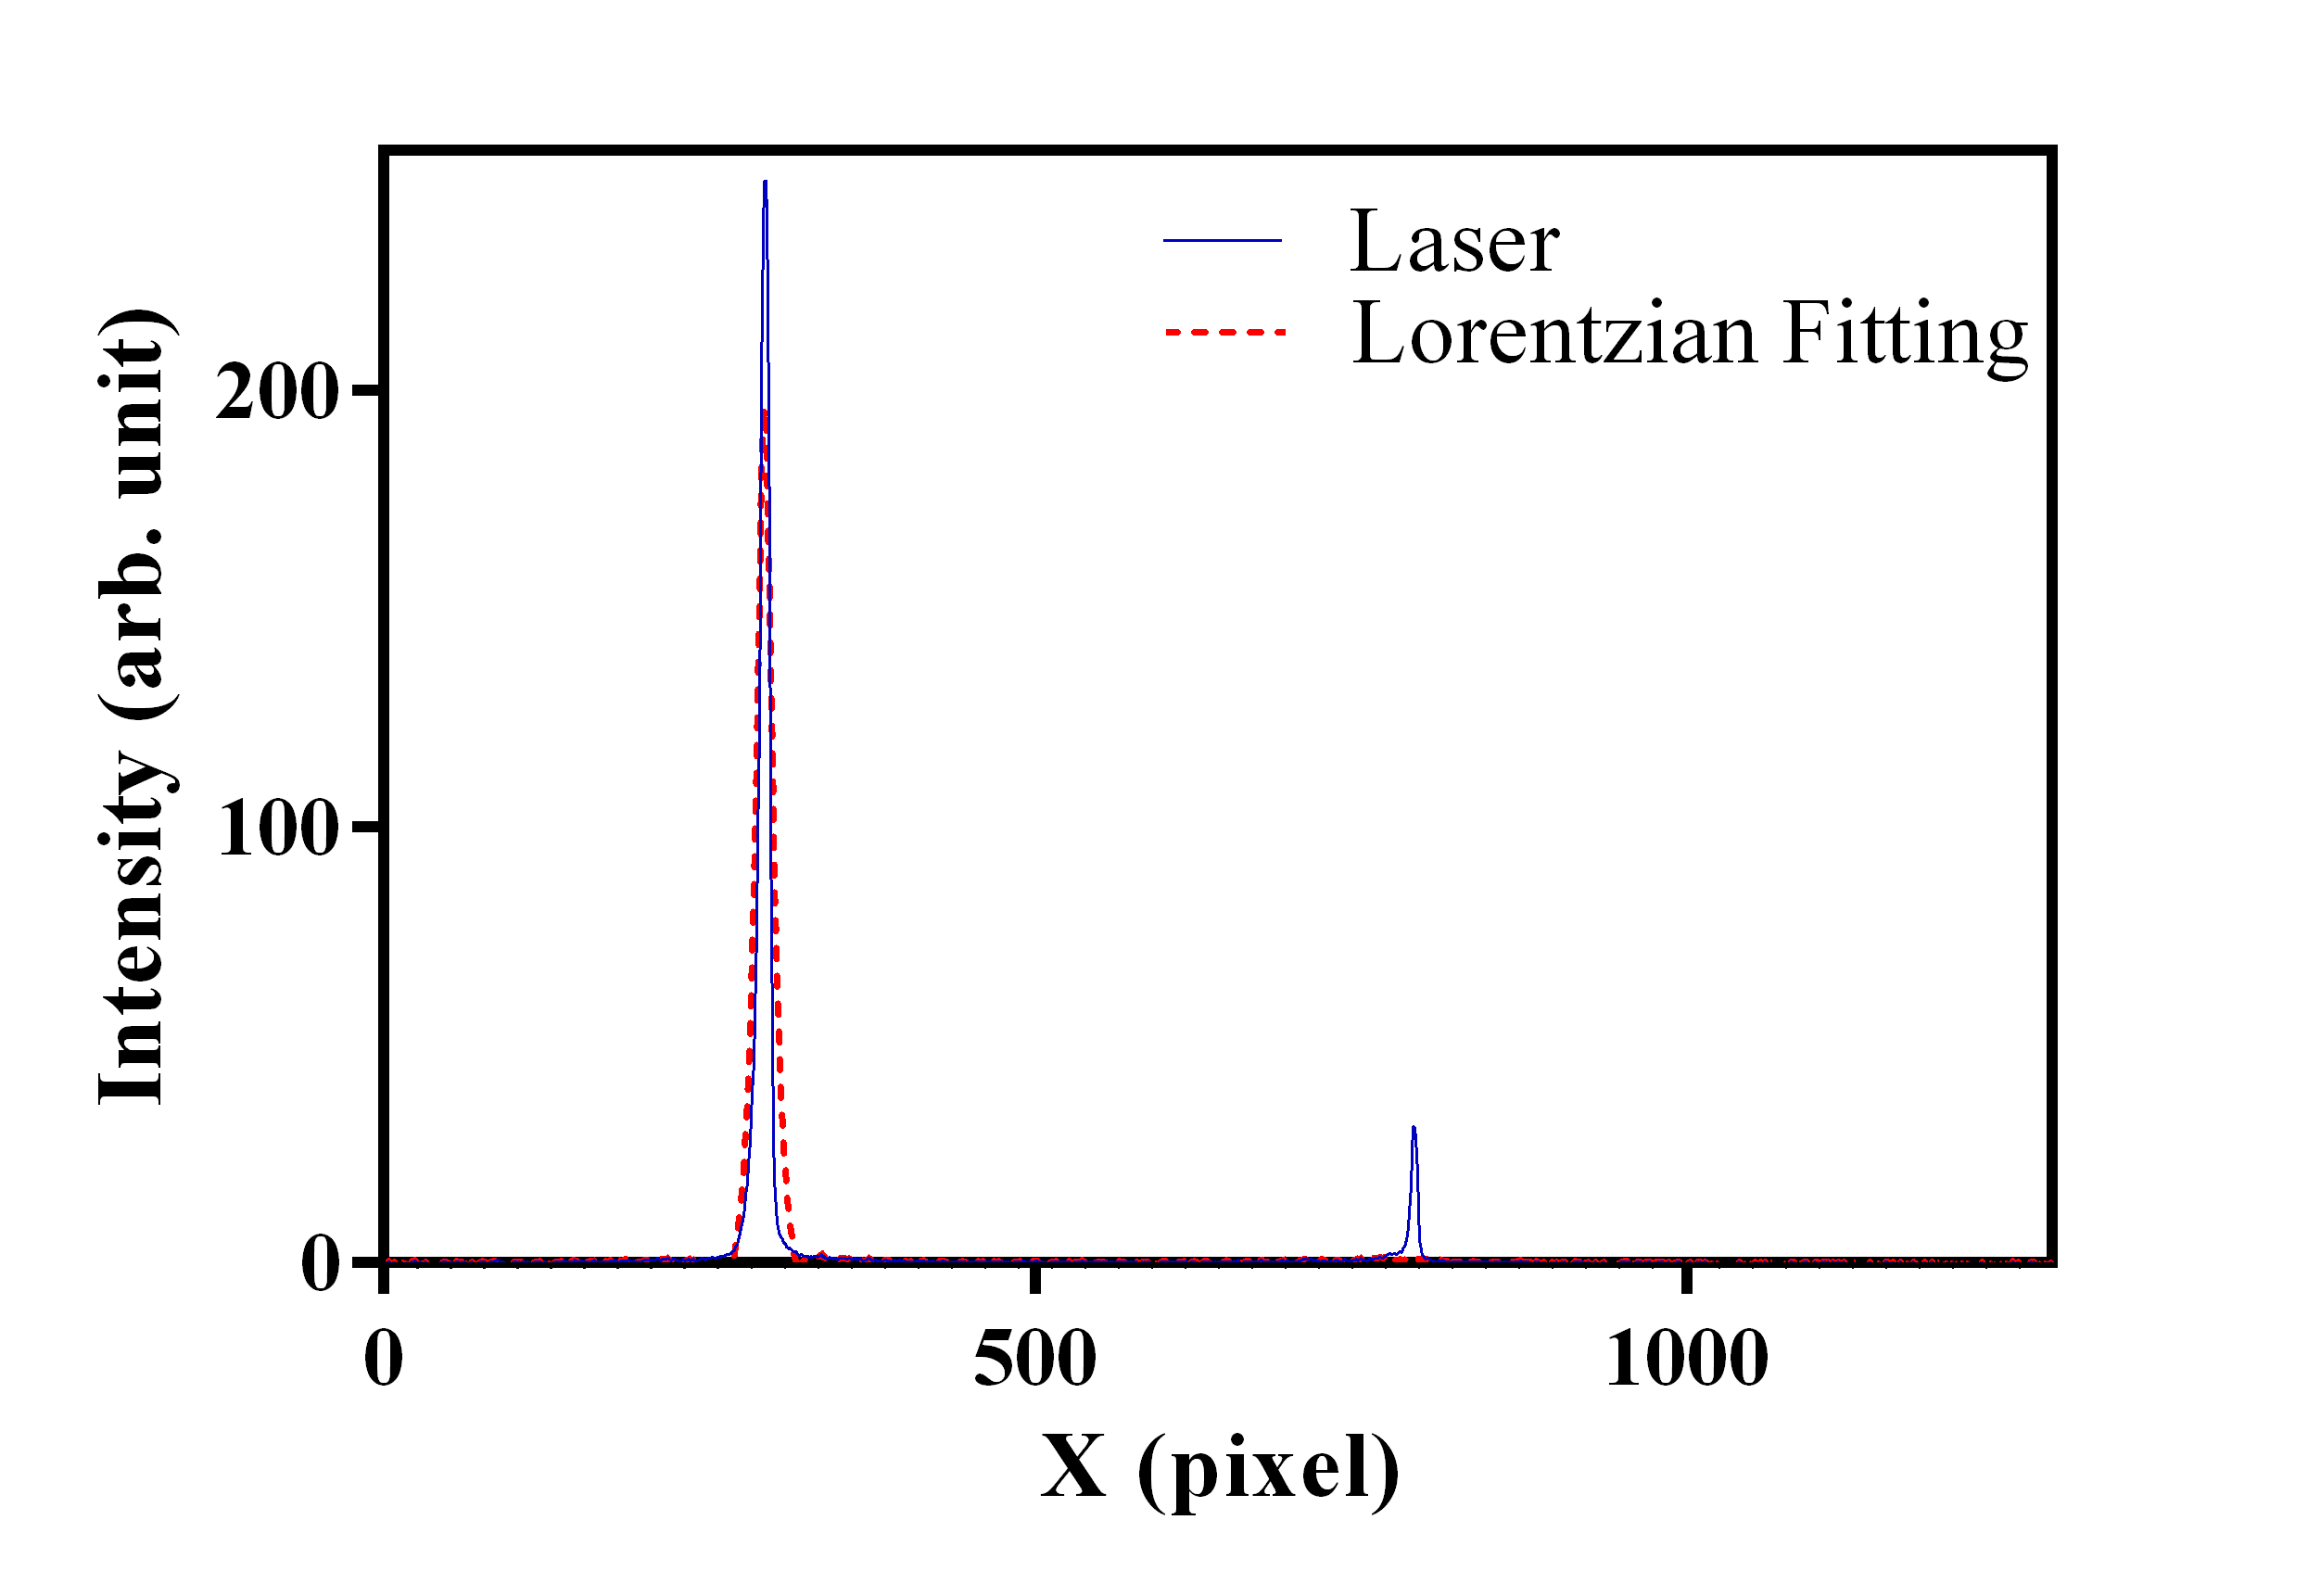
\includegraphics[width=\textwidth]{figures/L1_Lorentz.png} %插入图片,[]中设置图片大小,{}中是图片文件名
	\caption{雷射光譜主波峰區域進行勞倫茲擬合後結果圖} %最终文档中希望显示的图片标题
	\label{雷射光譜主波峰區域進行勞倫茲擬合後結果圖} %用于文内引用的标签
\end{figure}
將擬合後得出的波峰位置記憶於程式站存記憶體中,並依序個別對不同波長之雷射光源重複進行單雷射波峰位置偵測,直至取得所有雷射光源的準確波峰位置,所有雷射波峰偵測結果疊圖如圖\ref{所有單雷射光譜經單雷射波峰位置偵測後結果疊圖}. 所示,而所有雷射光譜由勞倫茲擬合後取得之準確波峰所在像素位置如表\ref{所有單雷射波峰經波峰偵測後所得出之參數表}. 所示。
\begin{figure}[H] %H为当前位置,!htb为忽略美学标准,htbp为浮动图形
	\centering %图片居中
	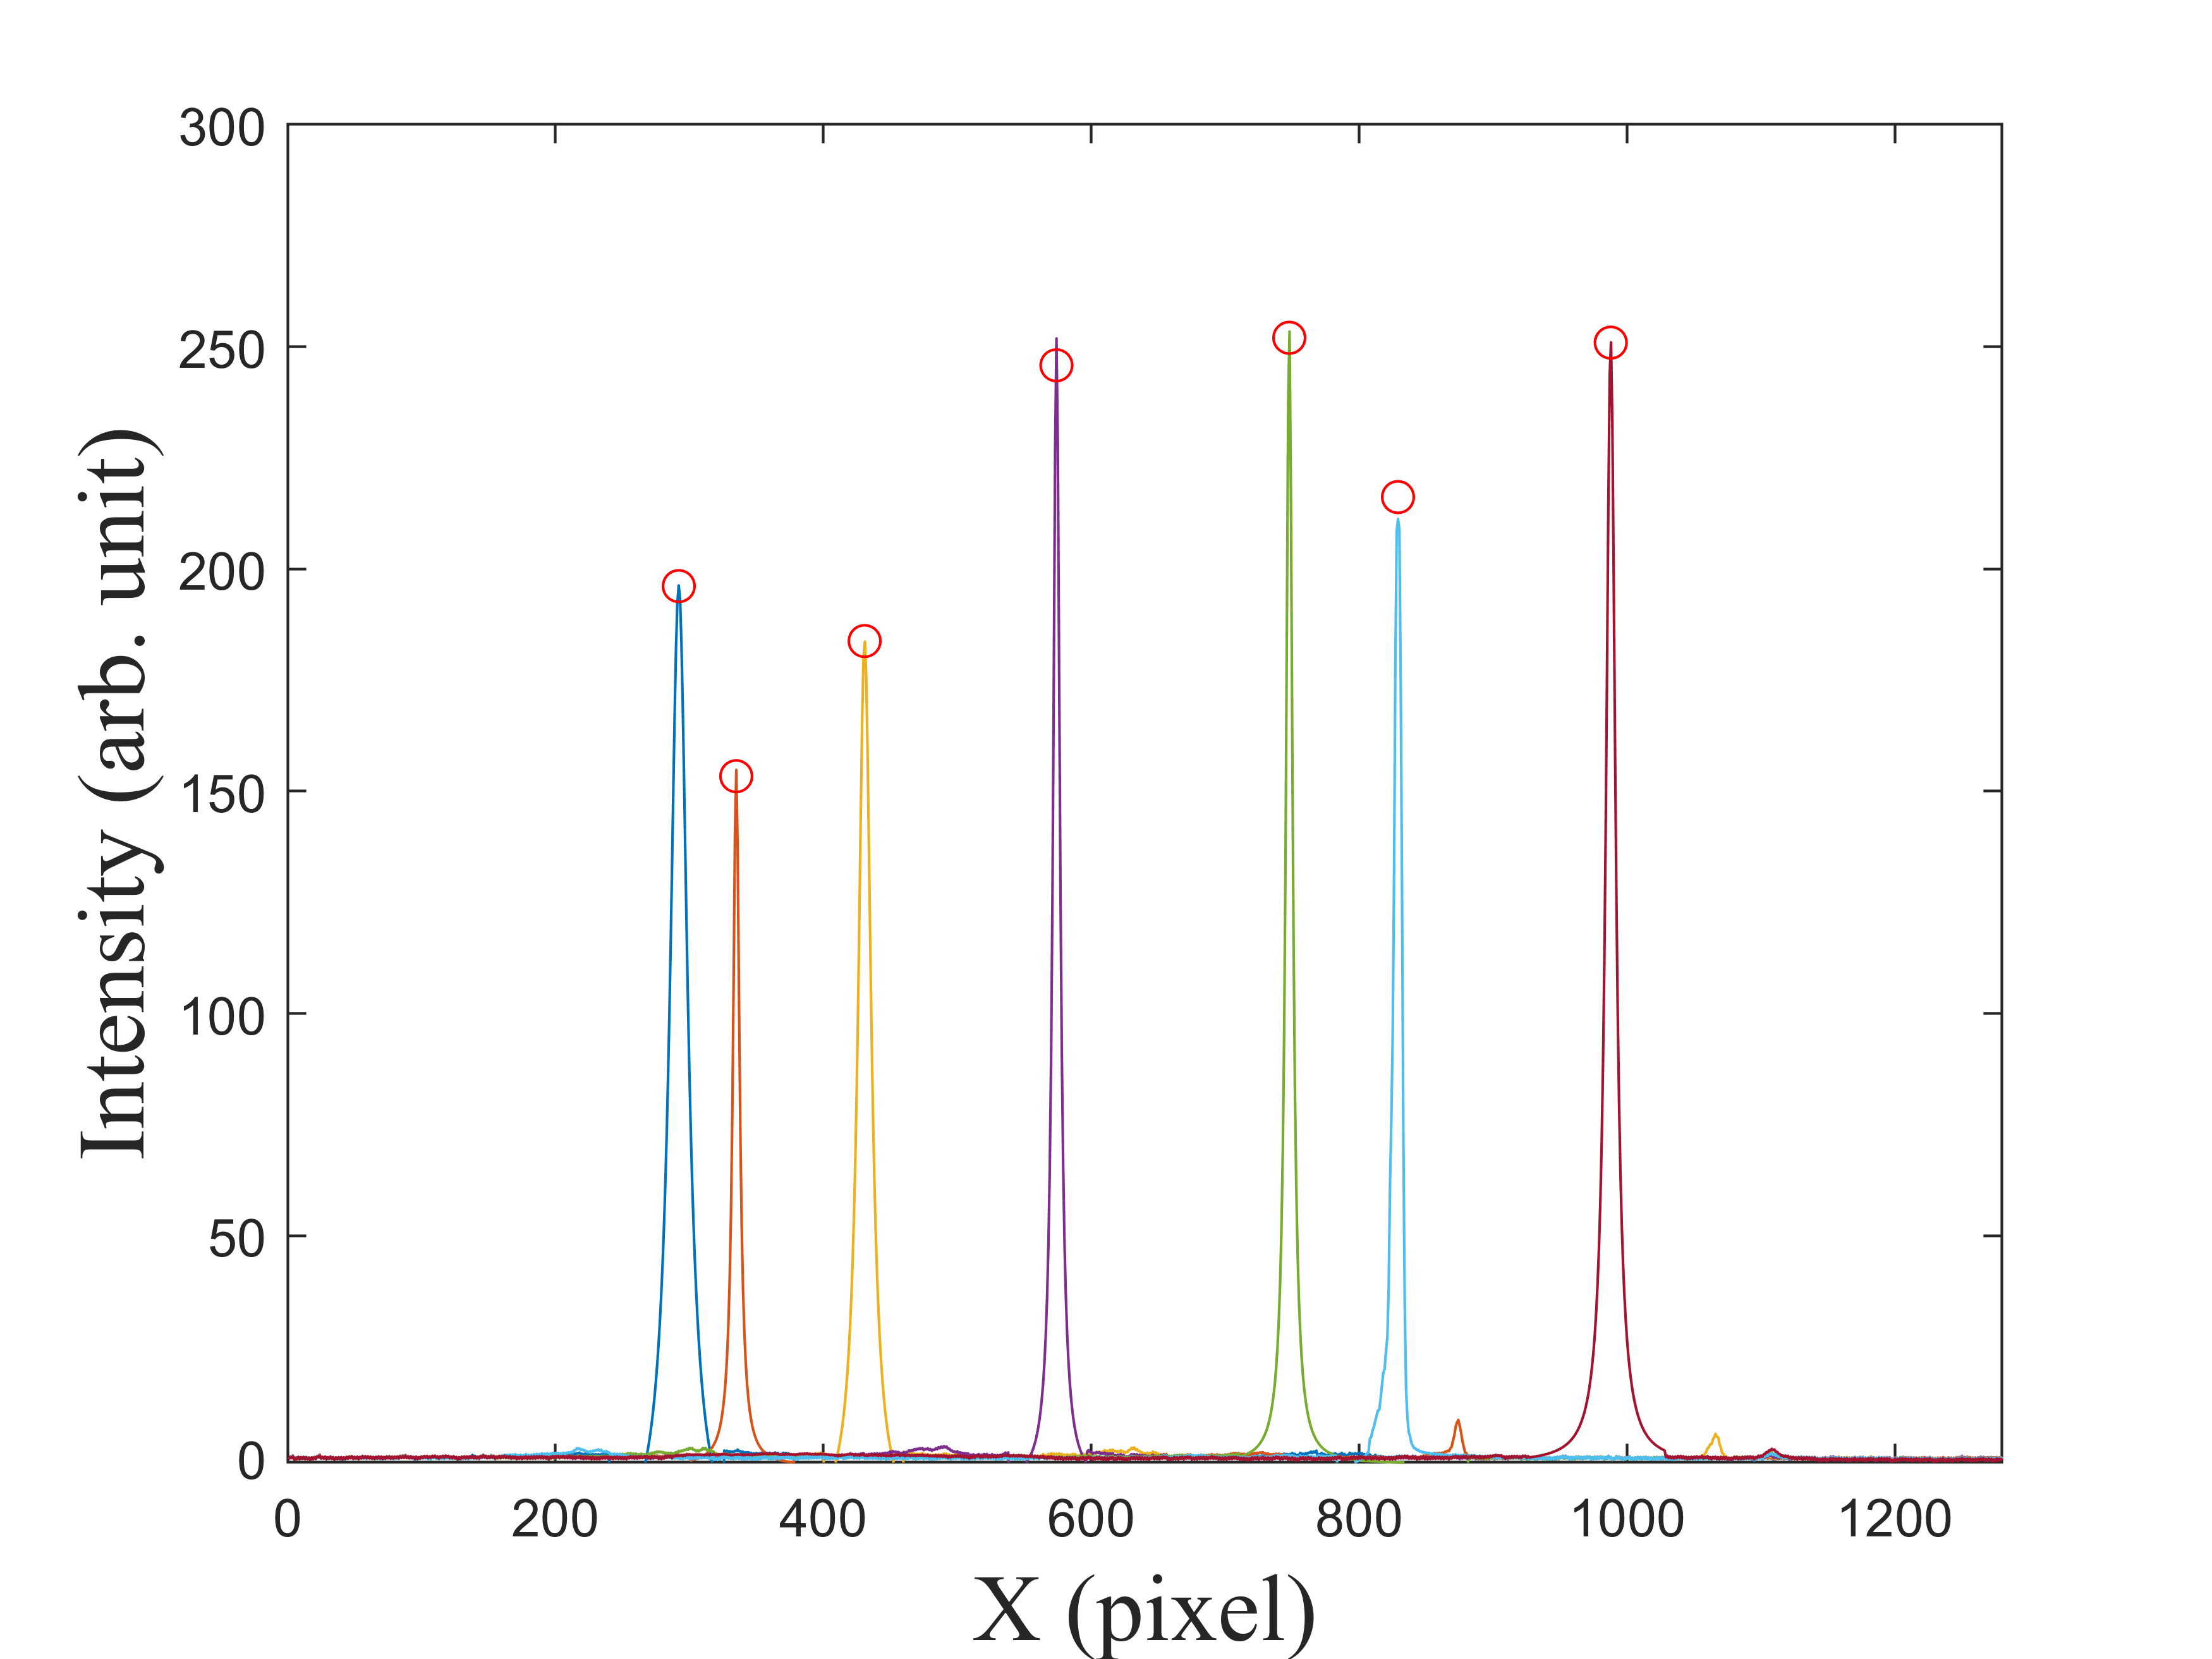
\includegraphics[width=16cm]{figures/AllLaserPeak.png} %插入图片,[]中设置图片大小,{}中是图片文件名
	\caption{所有單雷射光譜經單雷射波峰位置偵測後結果疊圖} %最终文档中希望显示的图片标题
	\label{所有單雷射光譜經單雷射波峰位置偵測後結果疊圖} %用于文内引用的标签
\end{figure}
\begin{center}
	\vspace{0.8cm}
	\captionof{table}{所有單雷射波峰經波峰偵測後所得出之參數表}\label{所有單雷射波峰經波峰偵測後所得出之參數表}
\begin{tabularx}{\textwidth}{m{0.2\textwidth}<{\centering}c m{0.25\textwidth}<{\centering}c}
	\hline\hline
	光源&峰值位置(pixel) & 強度 & 半高全寬(pixel)\\		
	\hline
	雷射1&292.0486	&196.1531&	12.8644\\
	雷射2&334.9441	&153.3864&	5.4504\\
	雷射3&430.7891	&183.7902&	9.5892\\
	雷射5&573.9681	&245.8263&	6.1762\\
	雷射6&747.8033	&252.0191&	5.5141\\
	雷射7&828.9508	&216.1823&	7.4330\\
	雷射8&987.7875	&250.9284&	7.5354\\
	\hline\hline
\end{tabularx}
\end{center}
\section{結合校正}
為了找出晶片空間轉換方程式,需要求出所有波峰的像素與其對應波長才能進行多項式擬合,而在透過一次次的波峰偵測後,現在已獲得所有汞氬燈與雷射目標波峰之準確的峰值所在像素位置,並且已知所有目標波峰與其對應的標準波長,將目標波峰像素位置與其對應標準波長表示於表\ref{所有目標波峰之峰值像素位置與標準波長對應表}. 中。
\begin{center}
	\vspace{0.8cm}
\captionof{table}{所有目標波峰之峰值像素位置與標準波長對應表}\label{所有目標波峰之峰值像素位置與標準波長對應表}
\begin{tabularx}{\textwidth}{m{0.3\textwidth}<{\centering}m{0.3\textwidth}<{\centering}m{0.3\textwidth}<{\centering}}
	\hline\hline
	光源&峰值位置(pixel) & 標準波長 (nm)\\		
	\hline
	\multirow{4}{*}{汞燈 }
	&287.9697&	404.65\\
	&326.3158&	435.83\\
	&461.6027&	546.07\\
	&500.5412&	578.01\\
	\hline
	\multirow{2}{*}{氬燈 }
	&724.7514&	763.51\\
	&781.2286&	811.53\\  
	\hline	
	雷射1&292.0486	&404.97 \\
	雷射2&334.9441	&443.93 \\
	雷射3&430.7891	&520.69 \\
	雷射5&573.9681	&642.13 \\
	雷射6&747.8033	&784.46 \\
	雷射7&828.9508	&851.04 \\
	雷射8&987.7875	&981.67 \\
	\hline\hline
\end{tabularx}
\vspace{10pt}
\end{center}
將表\ref{所有目標波峰之峰值像素位置與標準波長對應表}. 中所有汞氬燈與雷射目標波峰之峰值像素位置以變數$P$表示,而與其對應之標準波長則以變數$\lambda$表示,將每一組對應變數結合成一組數據$(P_i,\lambda_i)$,則波長空間與像素空間之三次轉換公式為
\begin{equation}\label{eq3.3}
	\lambda_i= a_0+a_1 P_i+a_2 P_{i}^2+a_3 P_{i}^3
\end{equation}
將所有數據組帶入方程式(\ref{eq3.3})並以矩陣表示為
\begin{equation}\label{eq3.4}
	\begin{bmatrix} \lambda_1\\\lambda_2\\\lambda_3\\ \vdots\\\lambda_n\end{bmatrix} 
	\quad
	= 
	\quad
	\begin{bmatrix} 
		1&P_1&P_{1}^{2}&P_{1}^{3}\\
		1&P_2&P_{2}^{2}&P_{2}^{3}\\
		1&P_3&P_{3}^{2}&P_{3}^{3}\\
		\vdots&\vdots&\vdots\\
		1&P_n&P_{n}^{2}&P_{n}^{3}
	\end{bmatrix}
	\begin{bmatrix} a_0\\a_1\\a_2\\a_3 \end{bmatrix} 
\end{equation}
將矩陣方程式(\ref{eq3.4})簡記為
\begin{equation}\label{eq3.5}
	\Lambda = PA
\end{equation}
則空間轉換公式之參數矩陣$A$的最小二乘方解為:
\begin{equation}\label{eq3.6}
	A = (P^TP)^{-1}P^T \Lambda
\end{equation}
今將表\ref{所有目標波峰之峰值像素位置與標準波長對應表}. 中數據組帶入公式(\ref{eq3.3})至公式(\ref{eq3.6})中,計算後即得出此晶片獨有之波長校正轉換公式如式(\ref{eq:WCfunction})所示。
\begin{equation}\label{eq:WCfunction}
	\lambda_i = 170.6808383 + 0.798394509P_i + 5.05 \times 10^{-5}P_i^2 -2.80\times 10^{-8}P_i^3	
\end{equation}
則此光譜晶片模組之每一像素點於波長空間中對應波長,即可透過將每個像素點帶入式(\ref{eq:WCfunction})所求得,擬和曲線如圖\ref{空間轉換擬和曲線}. 所示。
\begin{figure}[H] %H为当前位置,!htb为忽略美学标准,htbp为浮动图形
	\centering %图片居中
	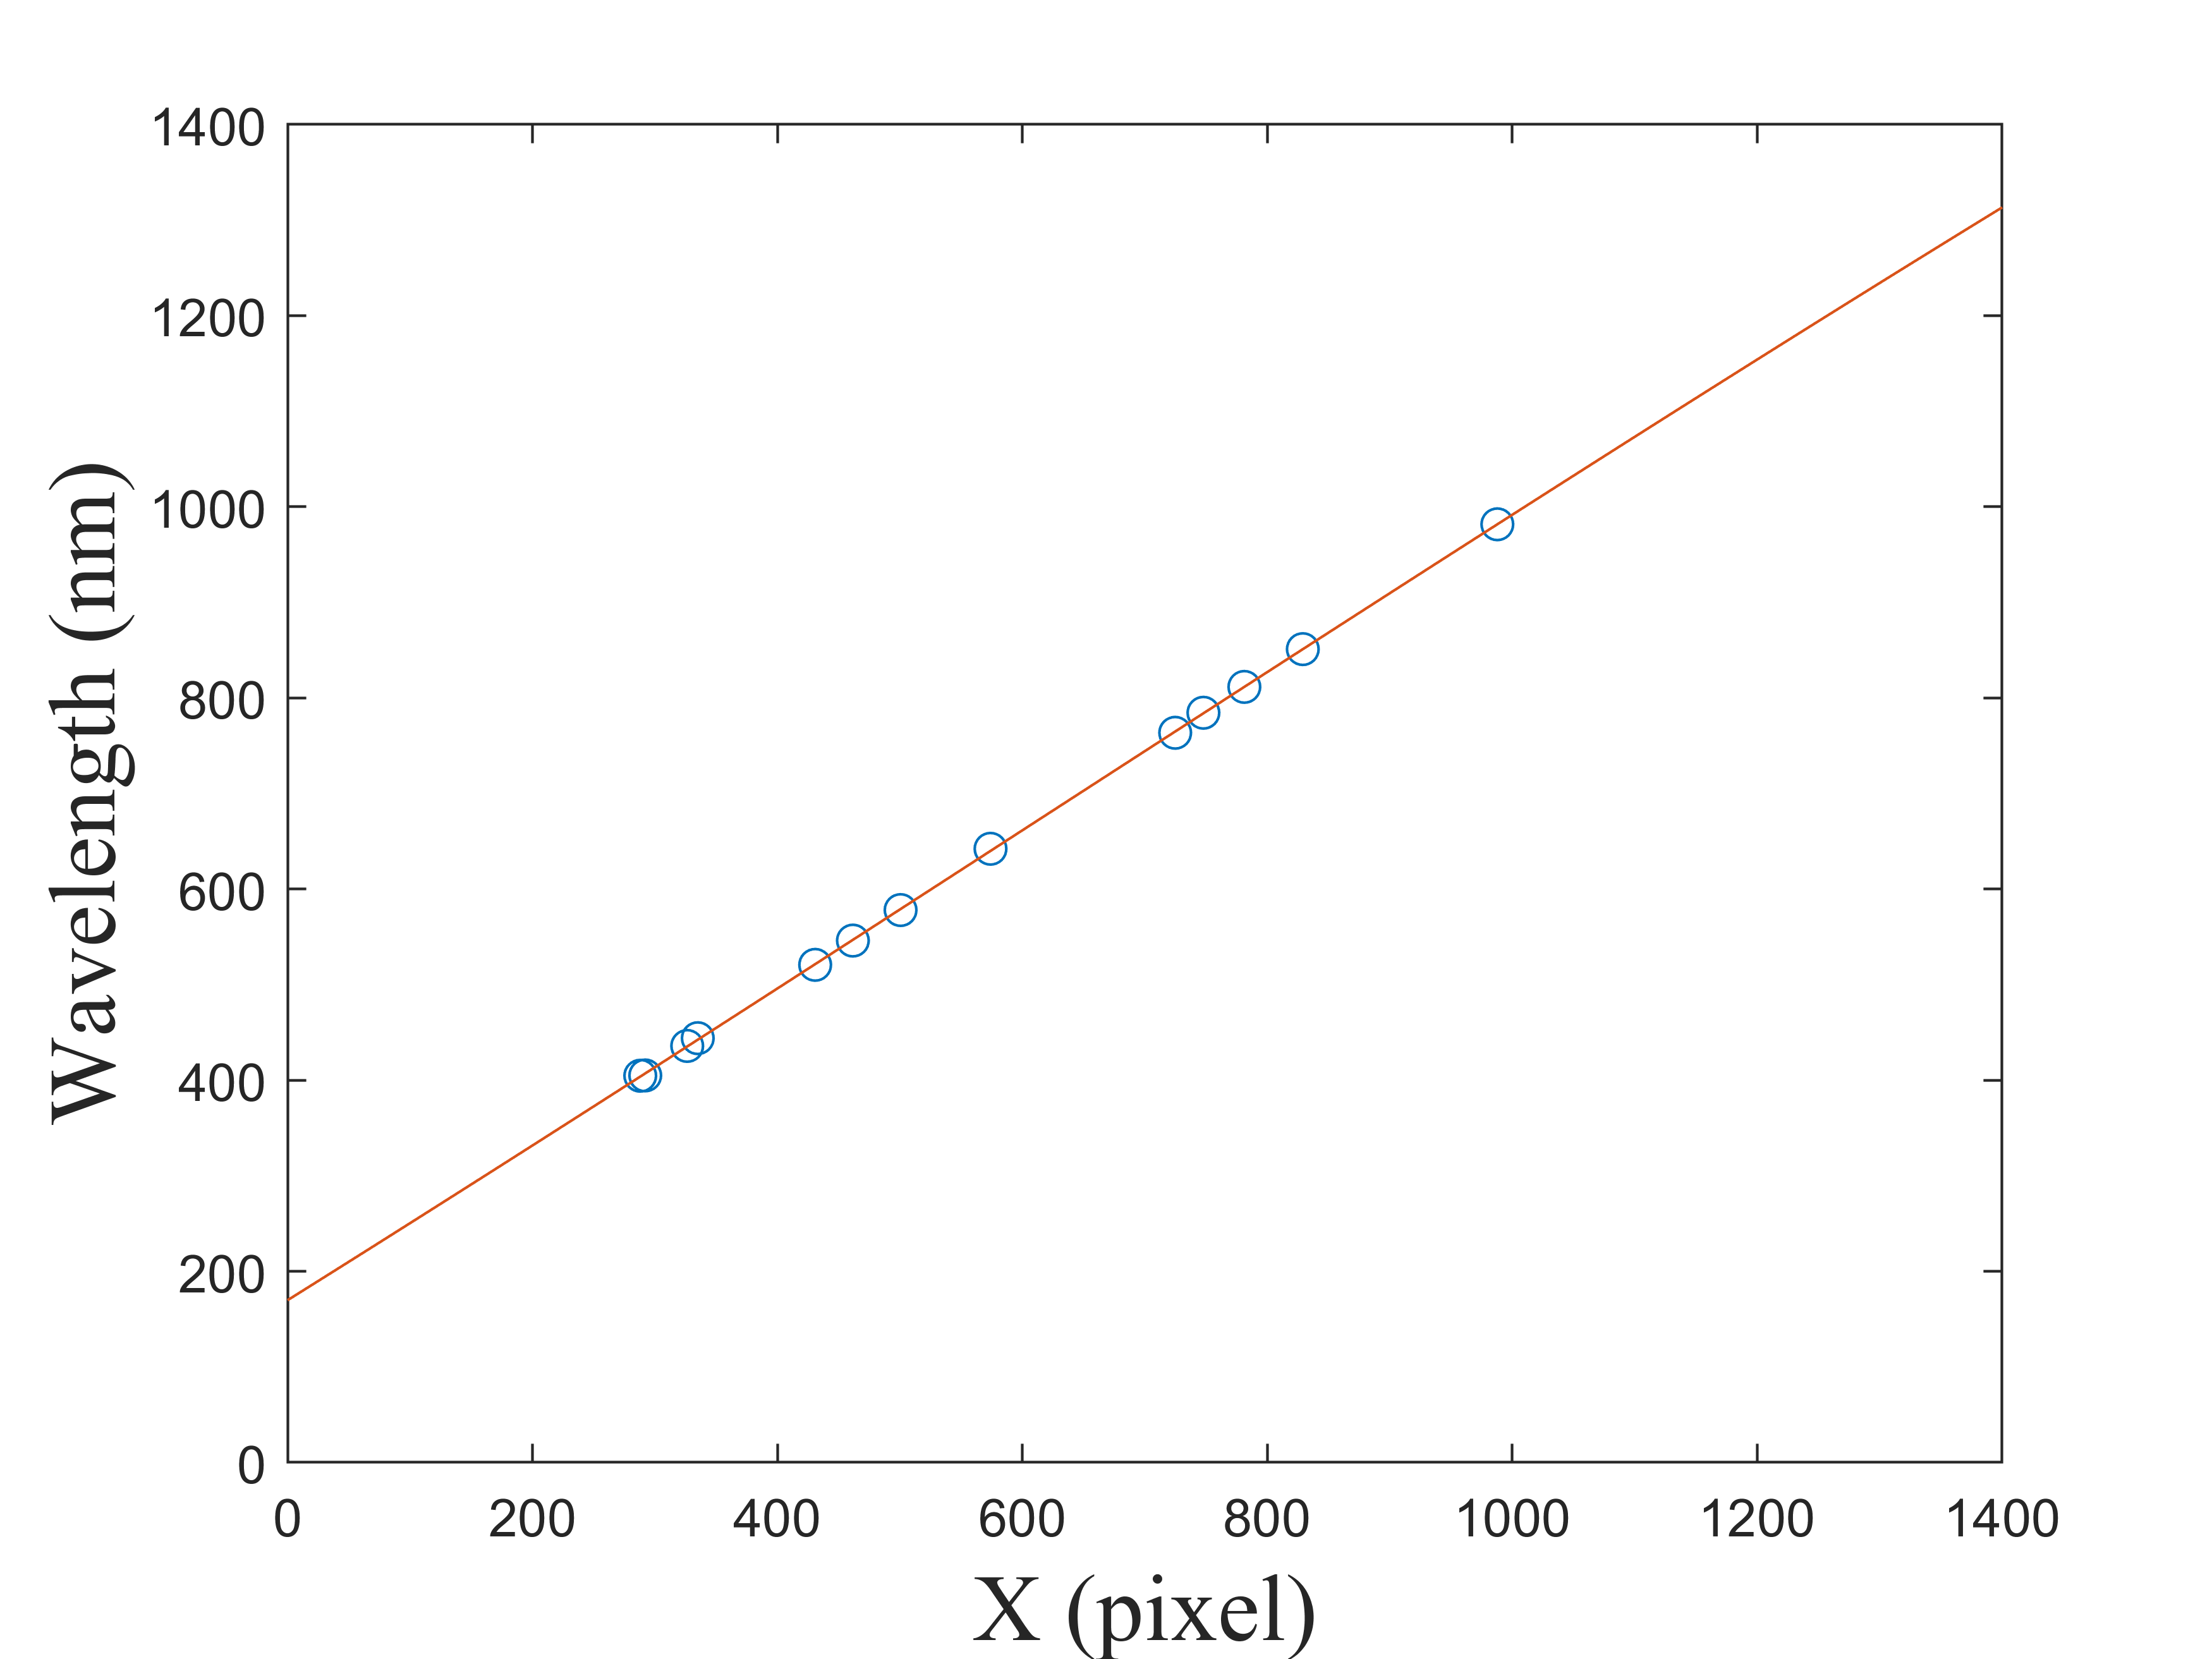
\includegraphics[width=16cm]{figures/COMBINE擬合結果.png} %插入图片,[]中设置图片大小,{}中是图片文件名
	\caption{空間轉換擬合曲線} %最终文档中希望显示的图片标题
	\label{空間轉換擬和曲線} %用于文内引用的标签
\end{figure}

\section{光譜晶片模組性能量化判定}
光譜晶片雖已經過波長校正,但並不能保證此光譜晶片品質優良,而光譜晶片的優劣將直接反映於光譜波形的表現上,汞氬燈這類原子光譜於理想的晶片下,半高全寬應趨近於零,而基線在不考慮電子雜訊干擾下,應平坦且趨近於零。\par
因晶片的性能優劣往往必須經由人工判定波形是否符合期待,但人工篩選常常參雜著主觀意見而標準不一,且耗時較長,因此為了使所有光譜晶片模組可以完全自動化校正並篩選,而在光源像素峰偵測流程時已計算出模型擬合與基線特徵點,因此本文提出將晶片性能以數值方式量化並提供篩選與判定。

\subsection{汞氬燈波形量化判定}
比較圖\ref{fig:all}. 中四張不同晶片之汞氬燈光譜,可以看出同樣於汞氬燈光源下,圖\ref{fig:a}. 晶片基線平整且半高全寬細,與其餘晶片的表現不同,顯然\ref{fig:d}. 晶片依然能以勞倫茲擬合後找出精準的波峰位置並波長校正,但圖\ref{fig:a}. 晶片波形表現明顯優於其餘晶片。

\begin{figure}[H]
	\vspace{0.8cm}
	\centering
	\begin{subfigure}[fig nice]{0.49\textwidth}
		\setlength{\abovecaptionskip}{0.cm}
		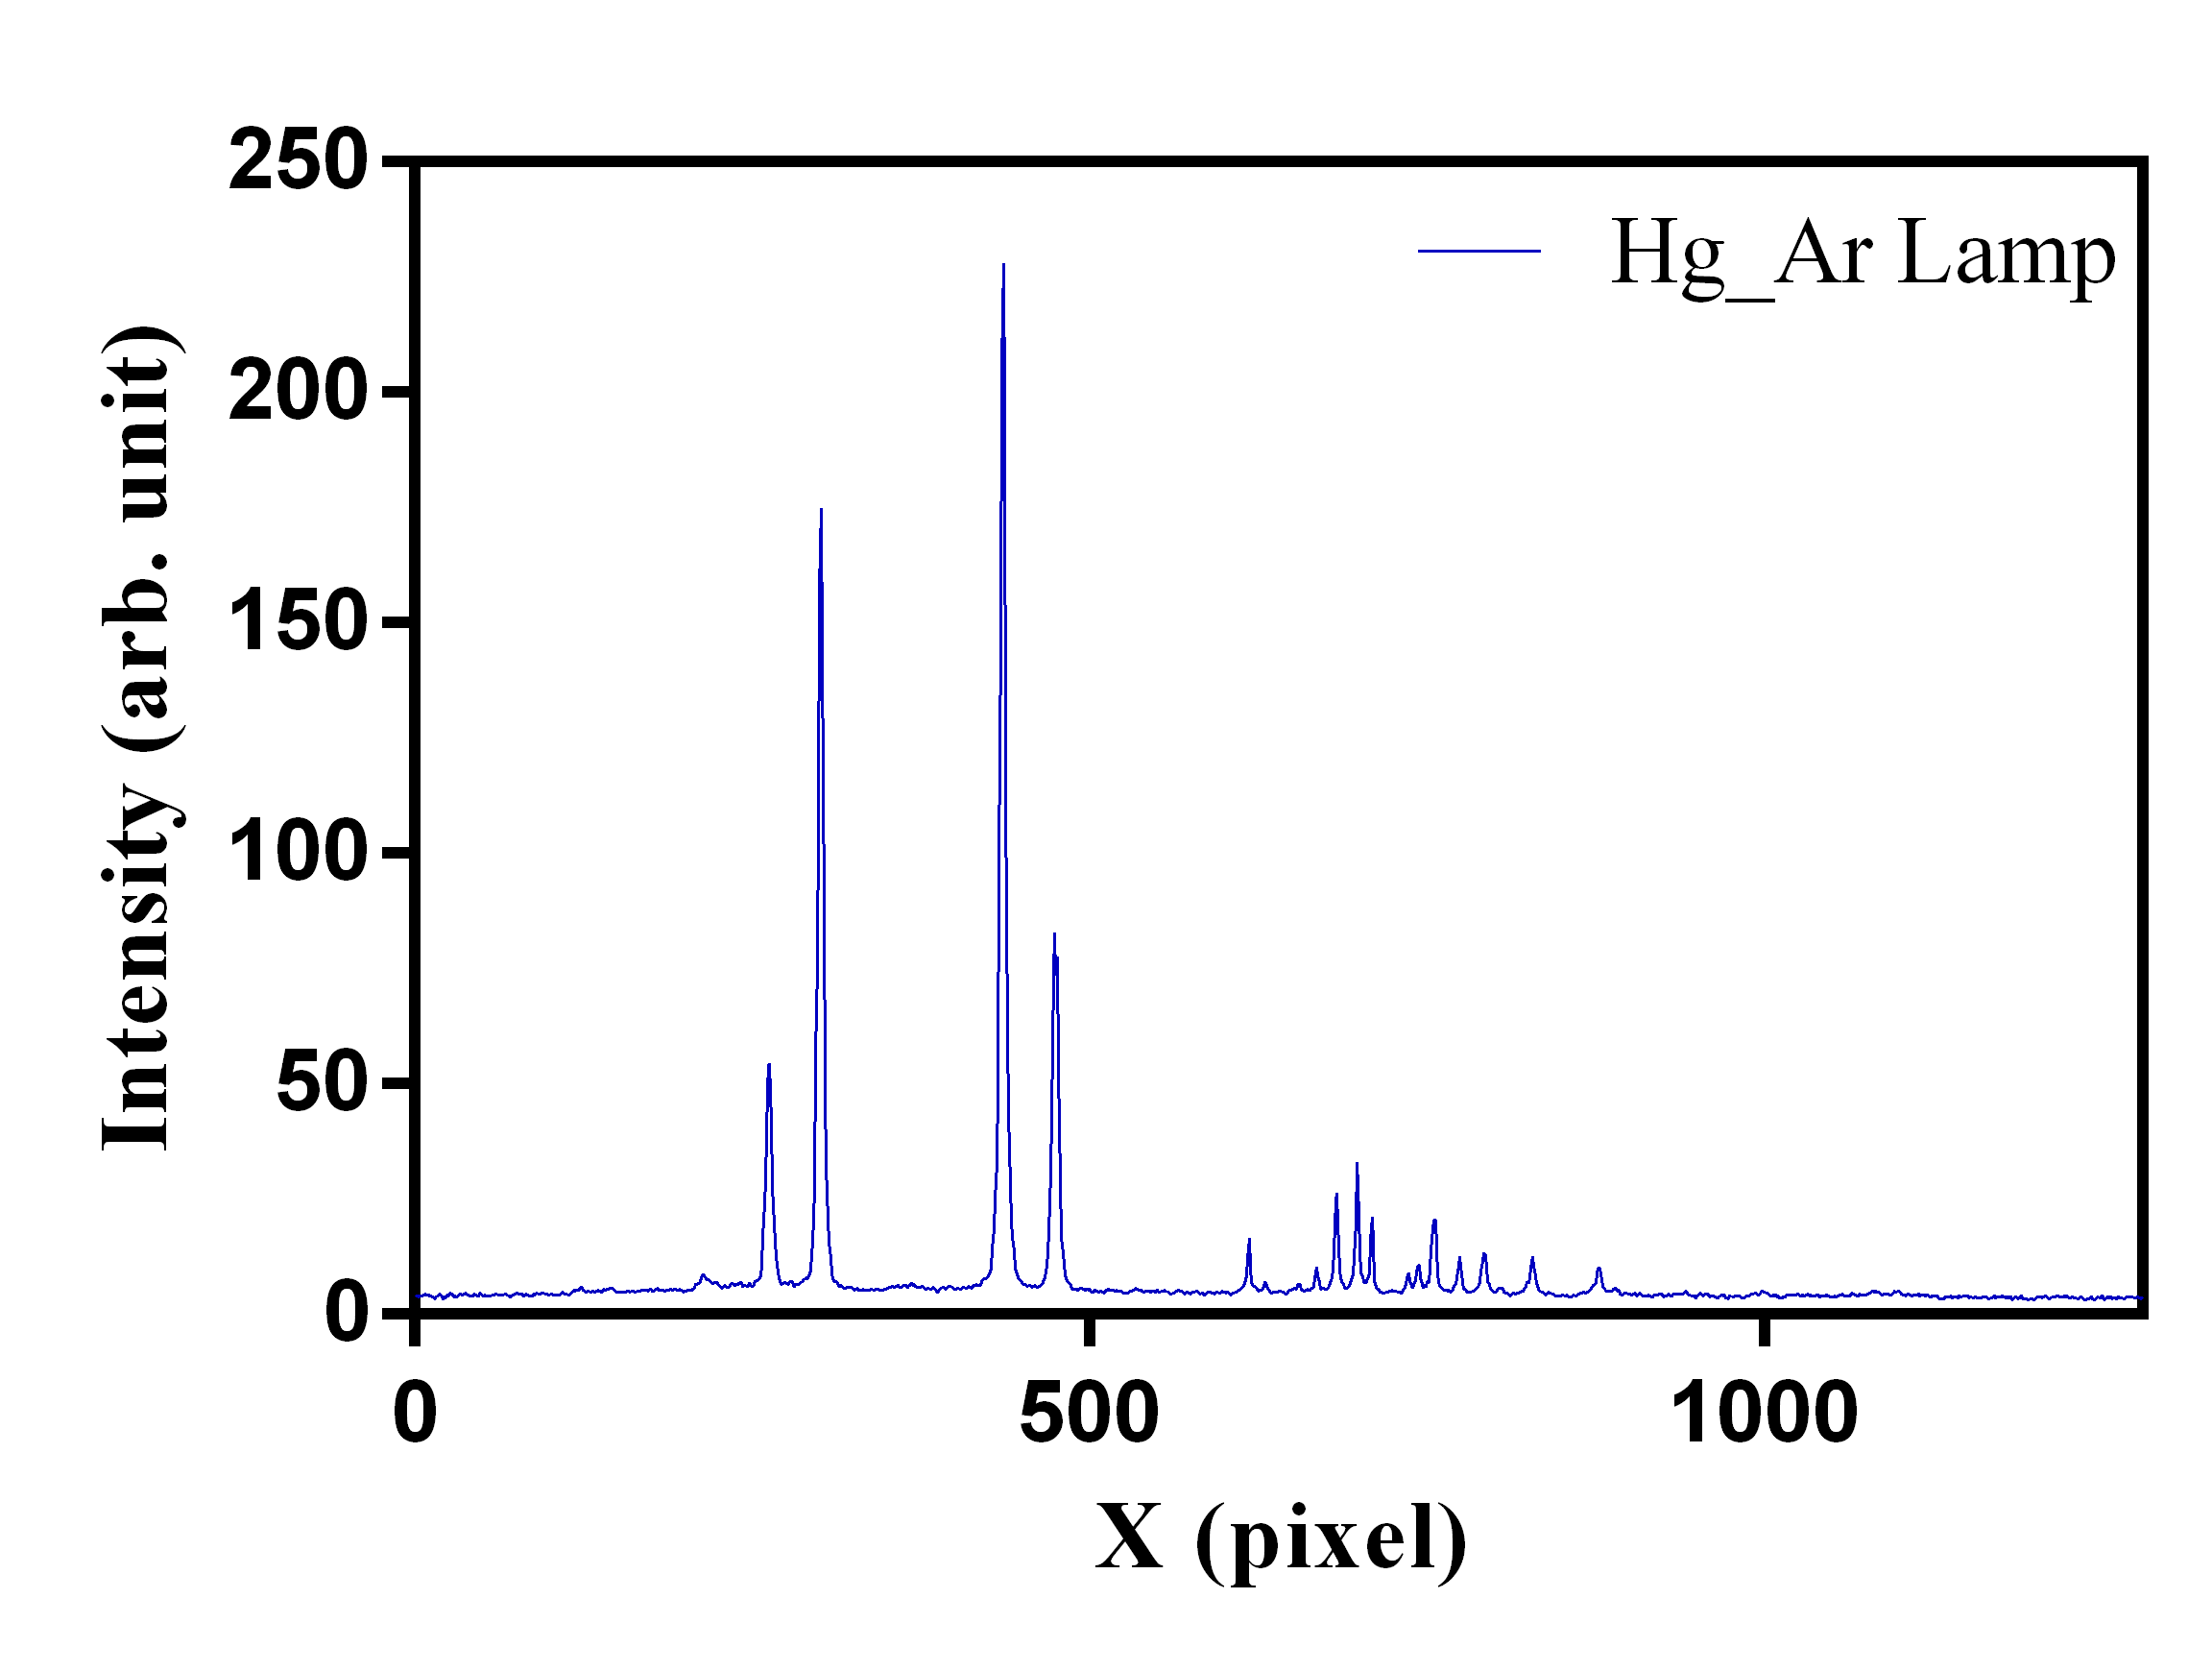
\includegraphics[width=7cm]{figures/hg_Nice.png}
		%\caption{優良晶片之汞氬燈光譜表現}
		\caption{}
		\label{fig:a}
	\end{subfigure}
\begin{subfigure}[fig nice]{0.49\textwidth}
	\setlength{\abovecaptionskip}{0.cm}
	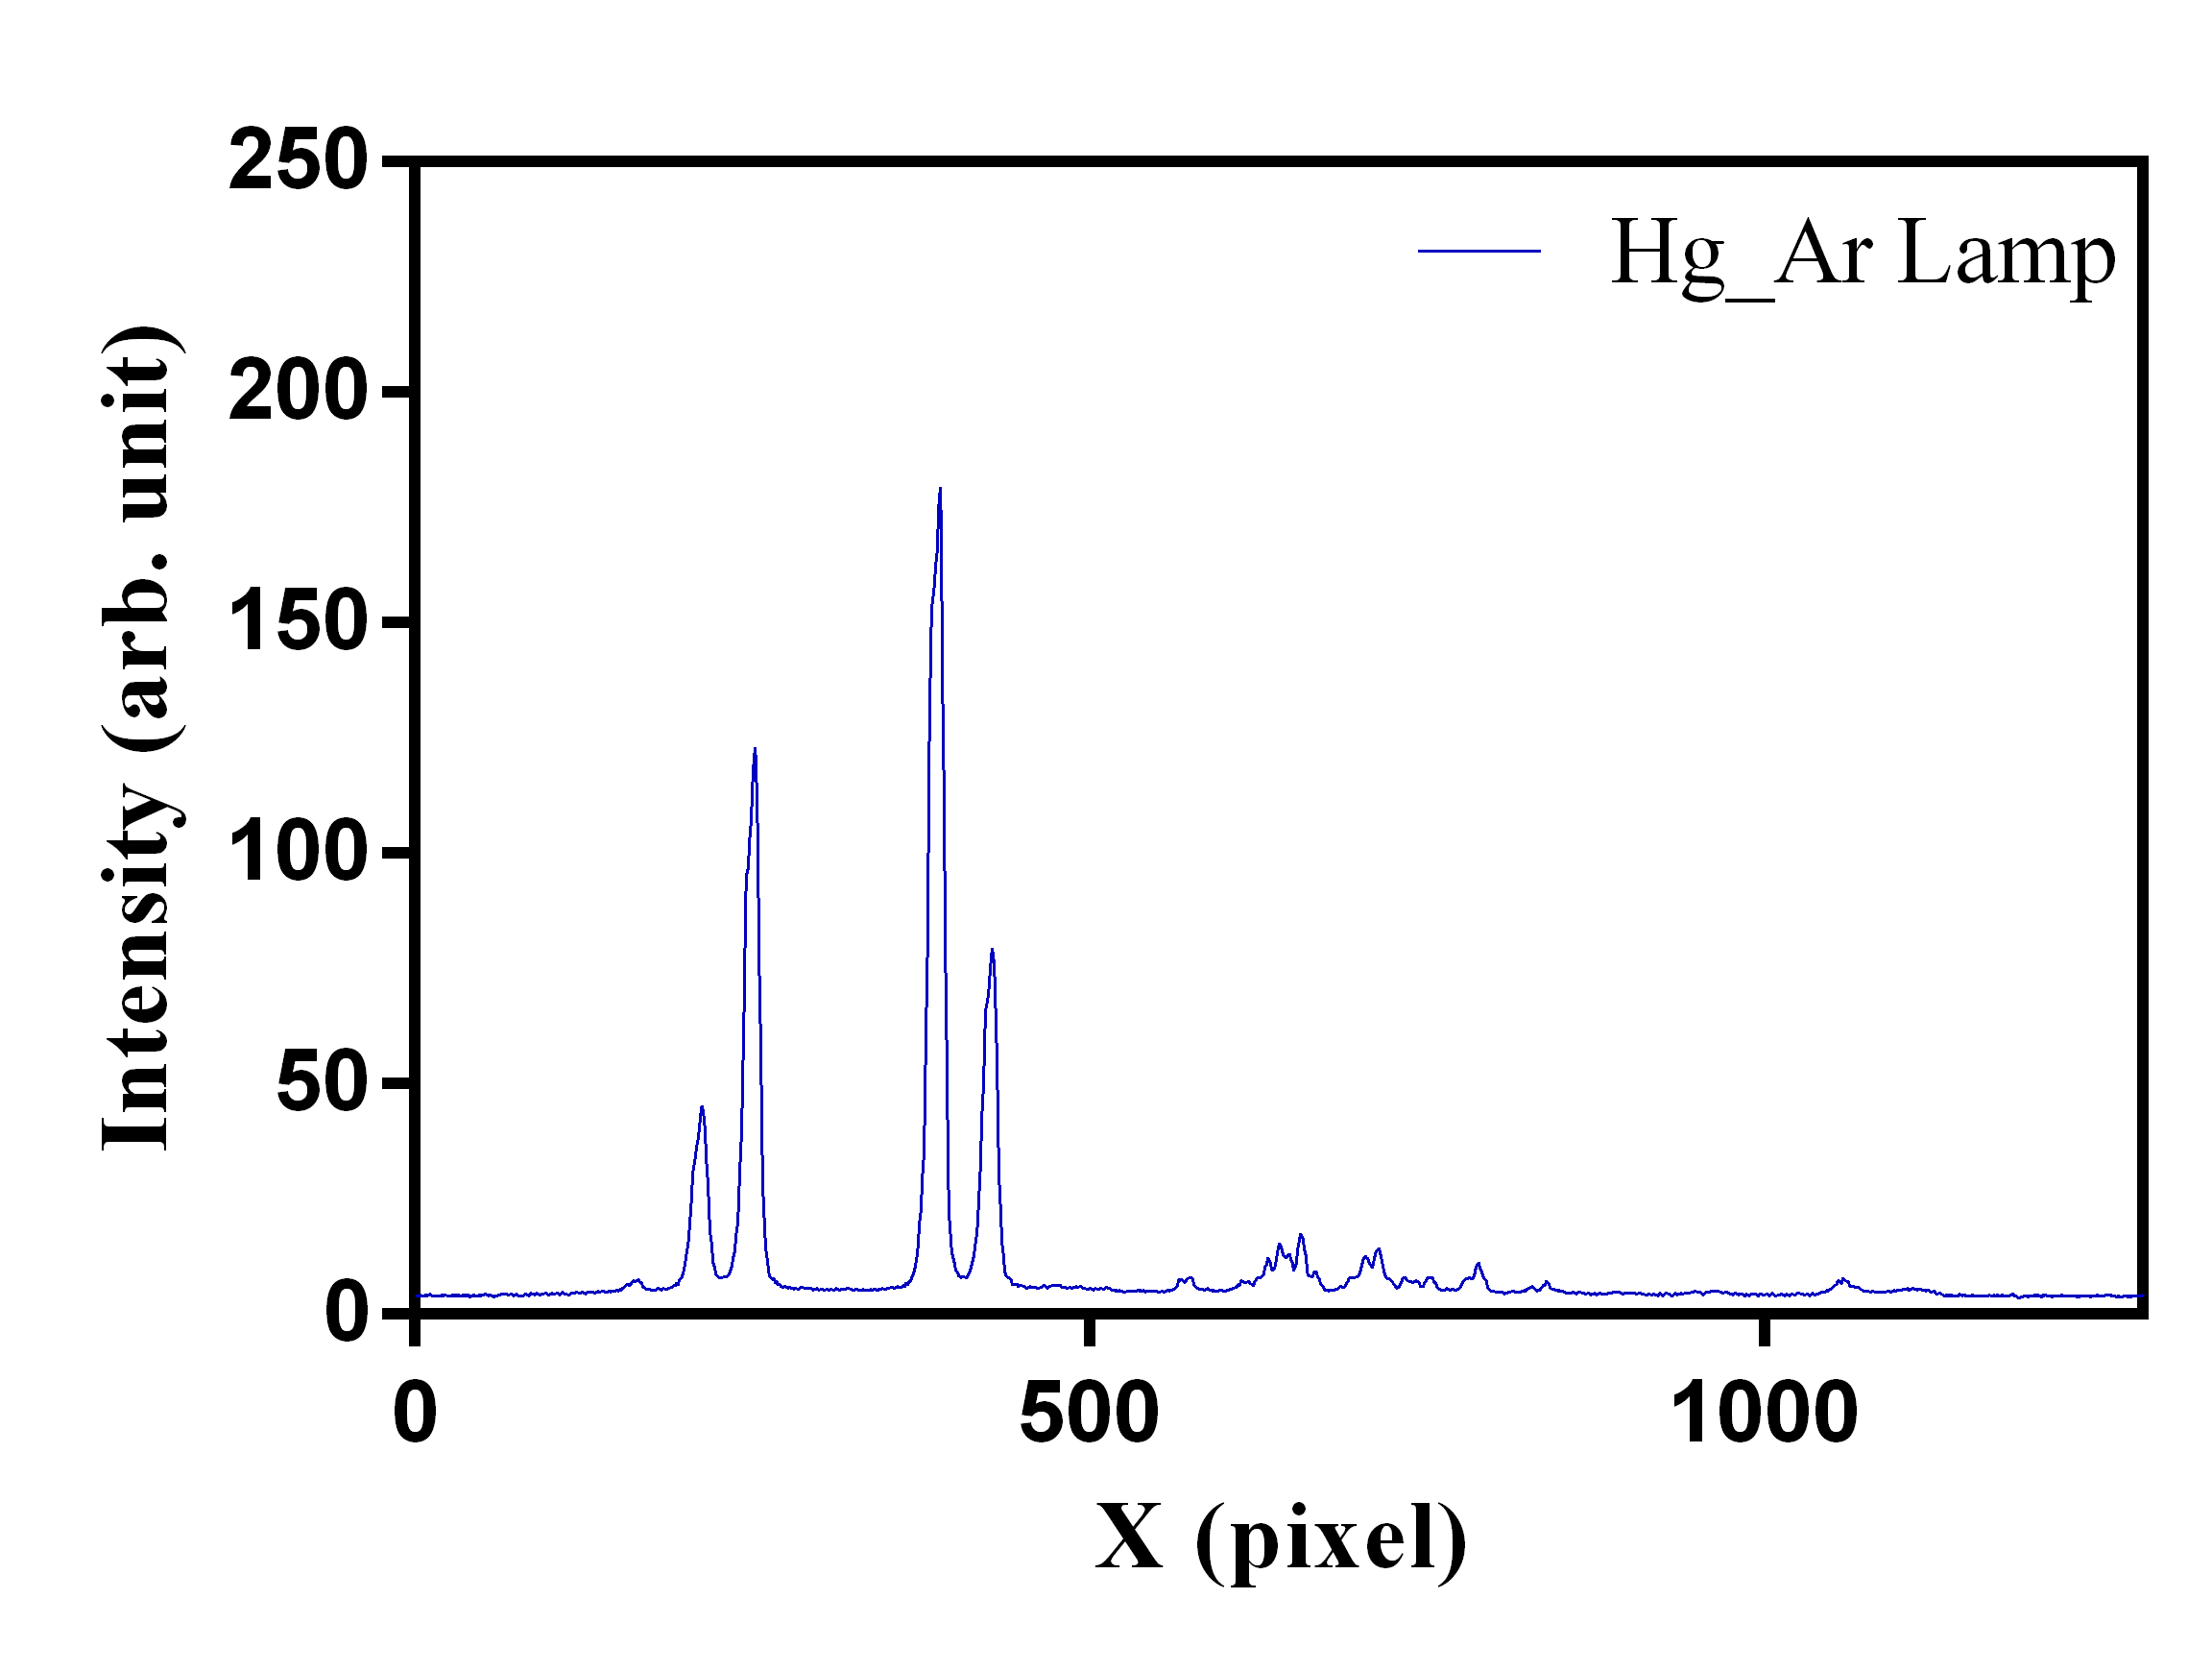
\includegraphics[width=7cm]{figures/hg_HWHM_BAD.png}
	%\caption{半高全寬較寬}
	\caption{}
	\label{fig:b}
\end{subfigure}
\begin{subfigure}[fig a]{0.49\textwidth}
	\setlength{\abovecaptionskip}{0.cm}
	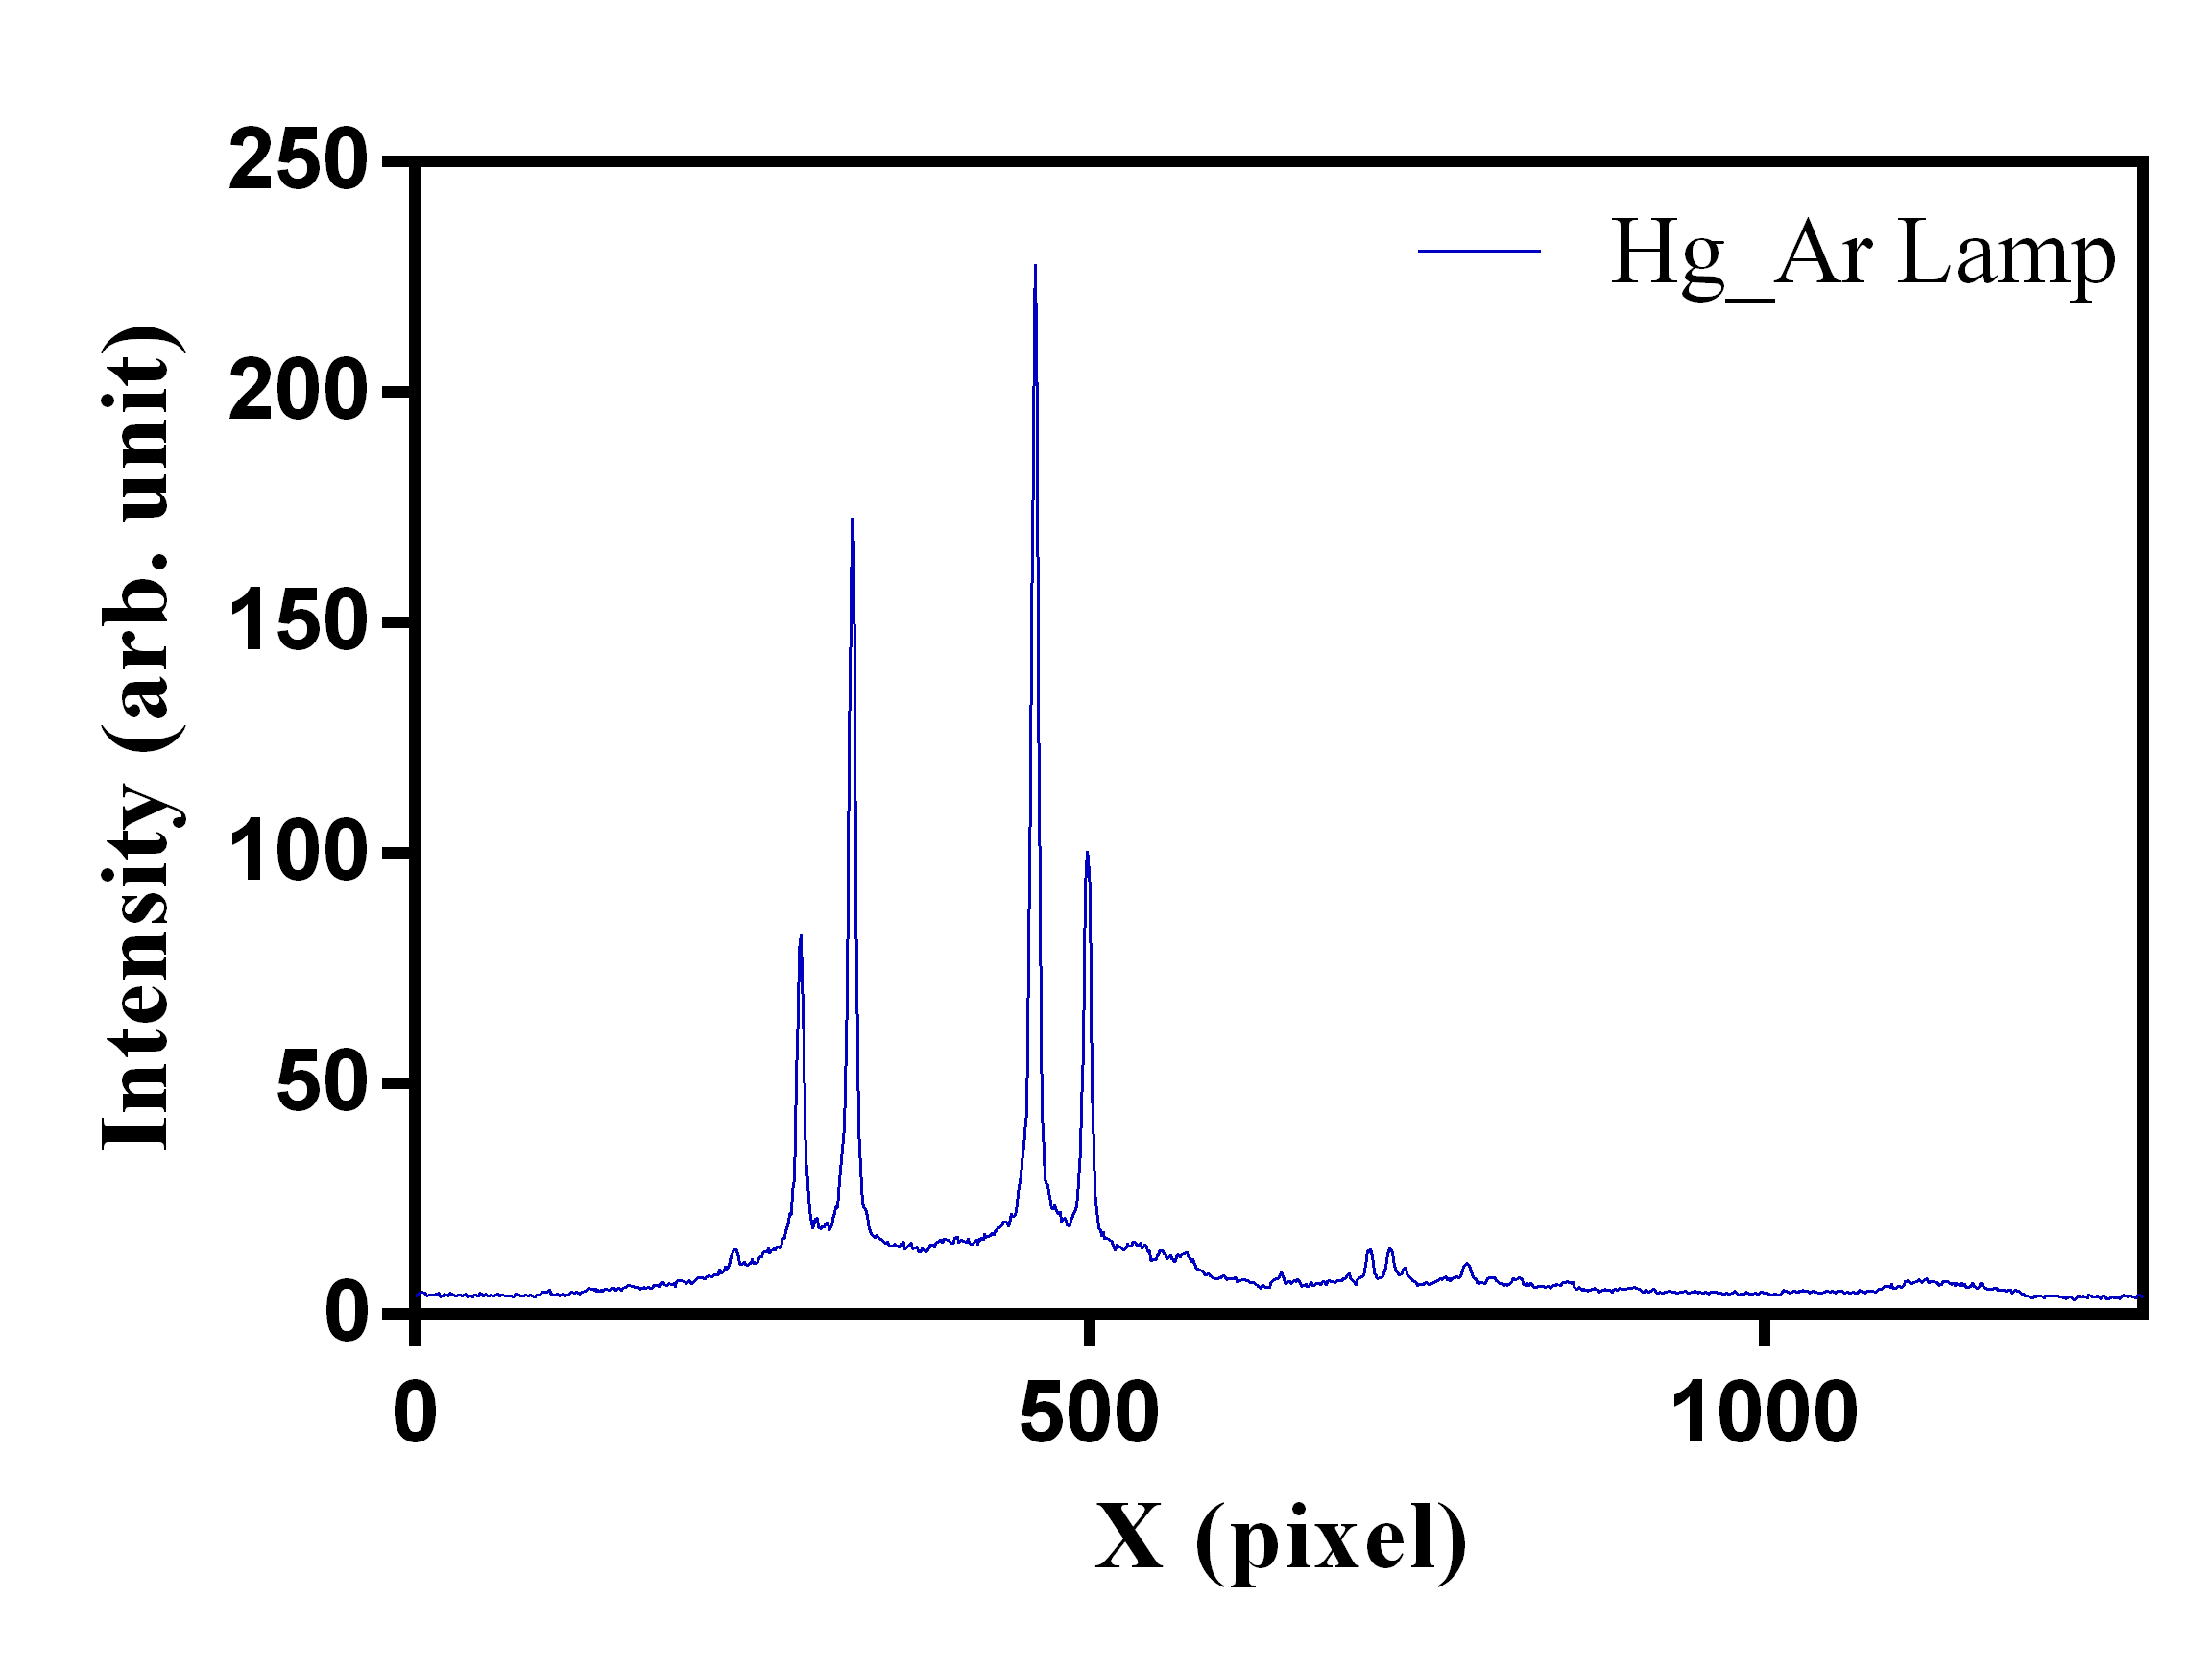
\includegraphics[width=7cm]{figures/hg_Baseline_bad.png}
	%\caption{基線較高}
	\caption{}
	\label{fig:c}
\end{subfigure}
\begin{subfigure}[fig b]{0.49\textwidth}
	\setlength{\abovecaptionskip}{0.cm}
	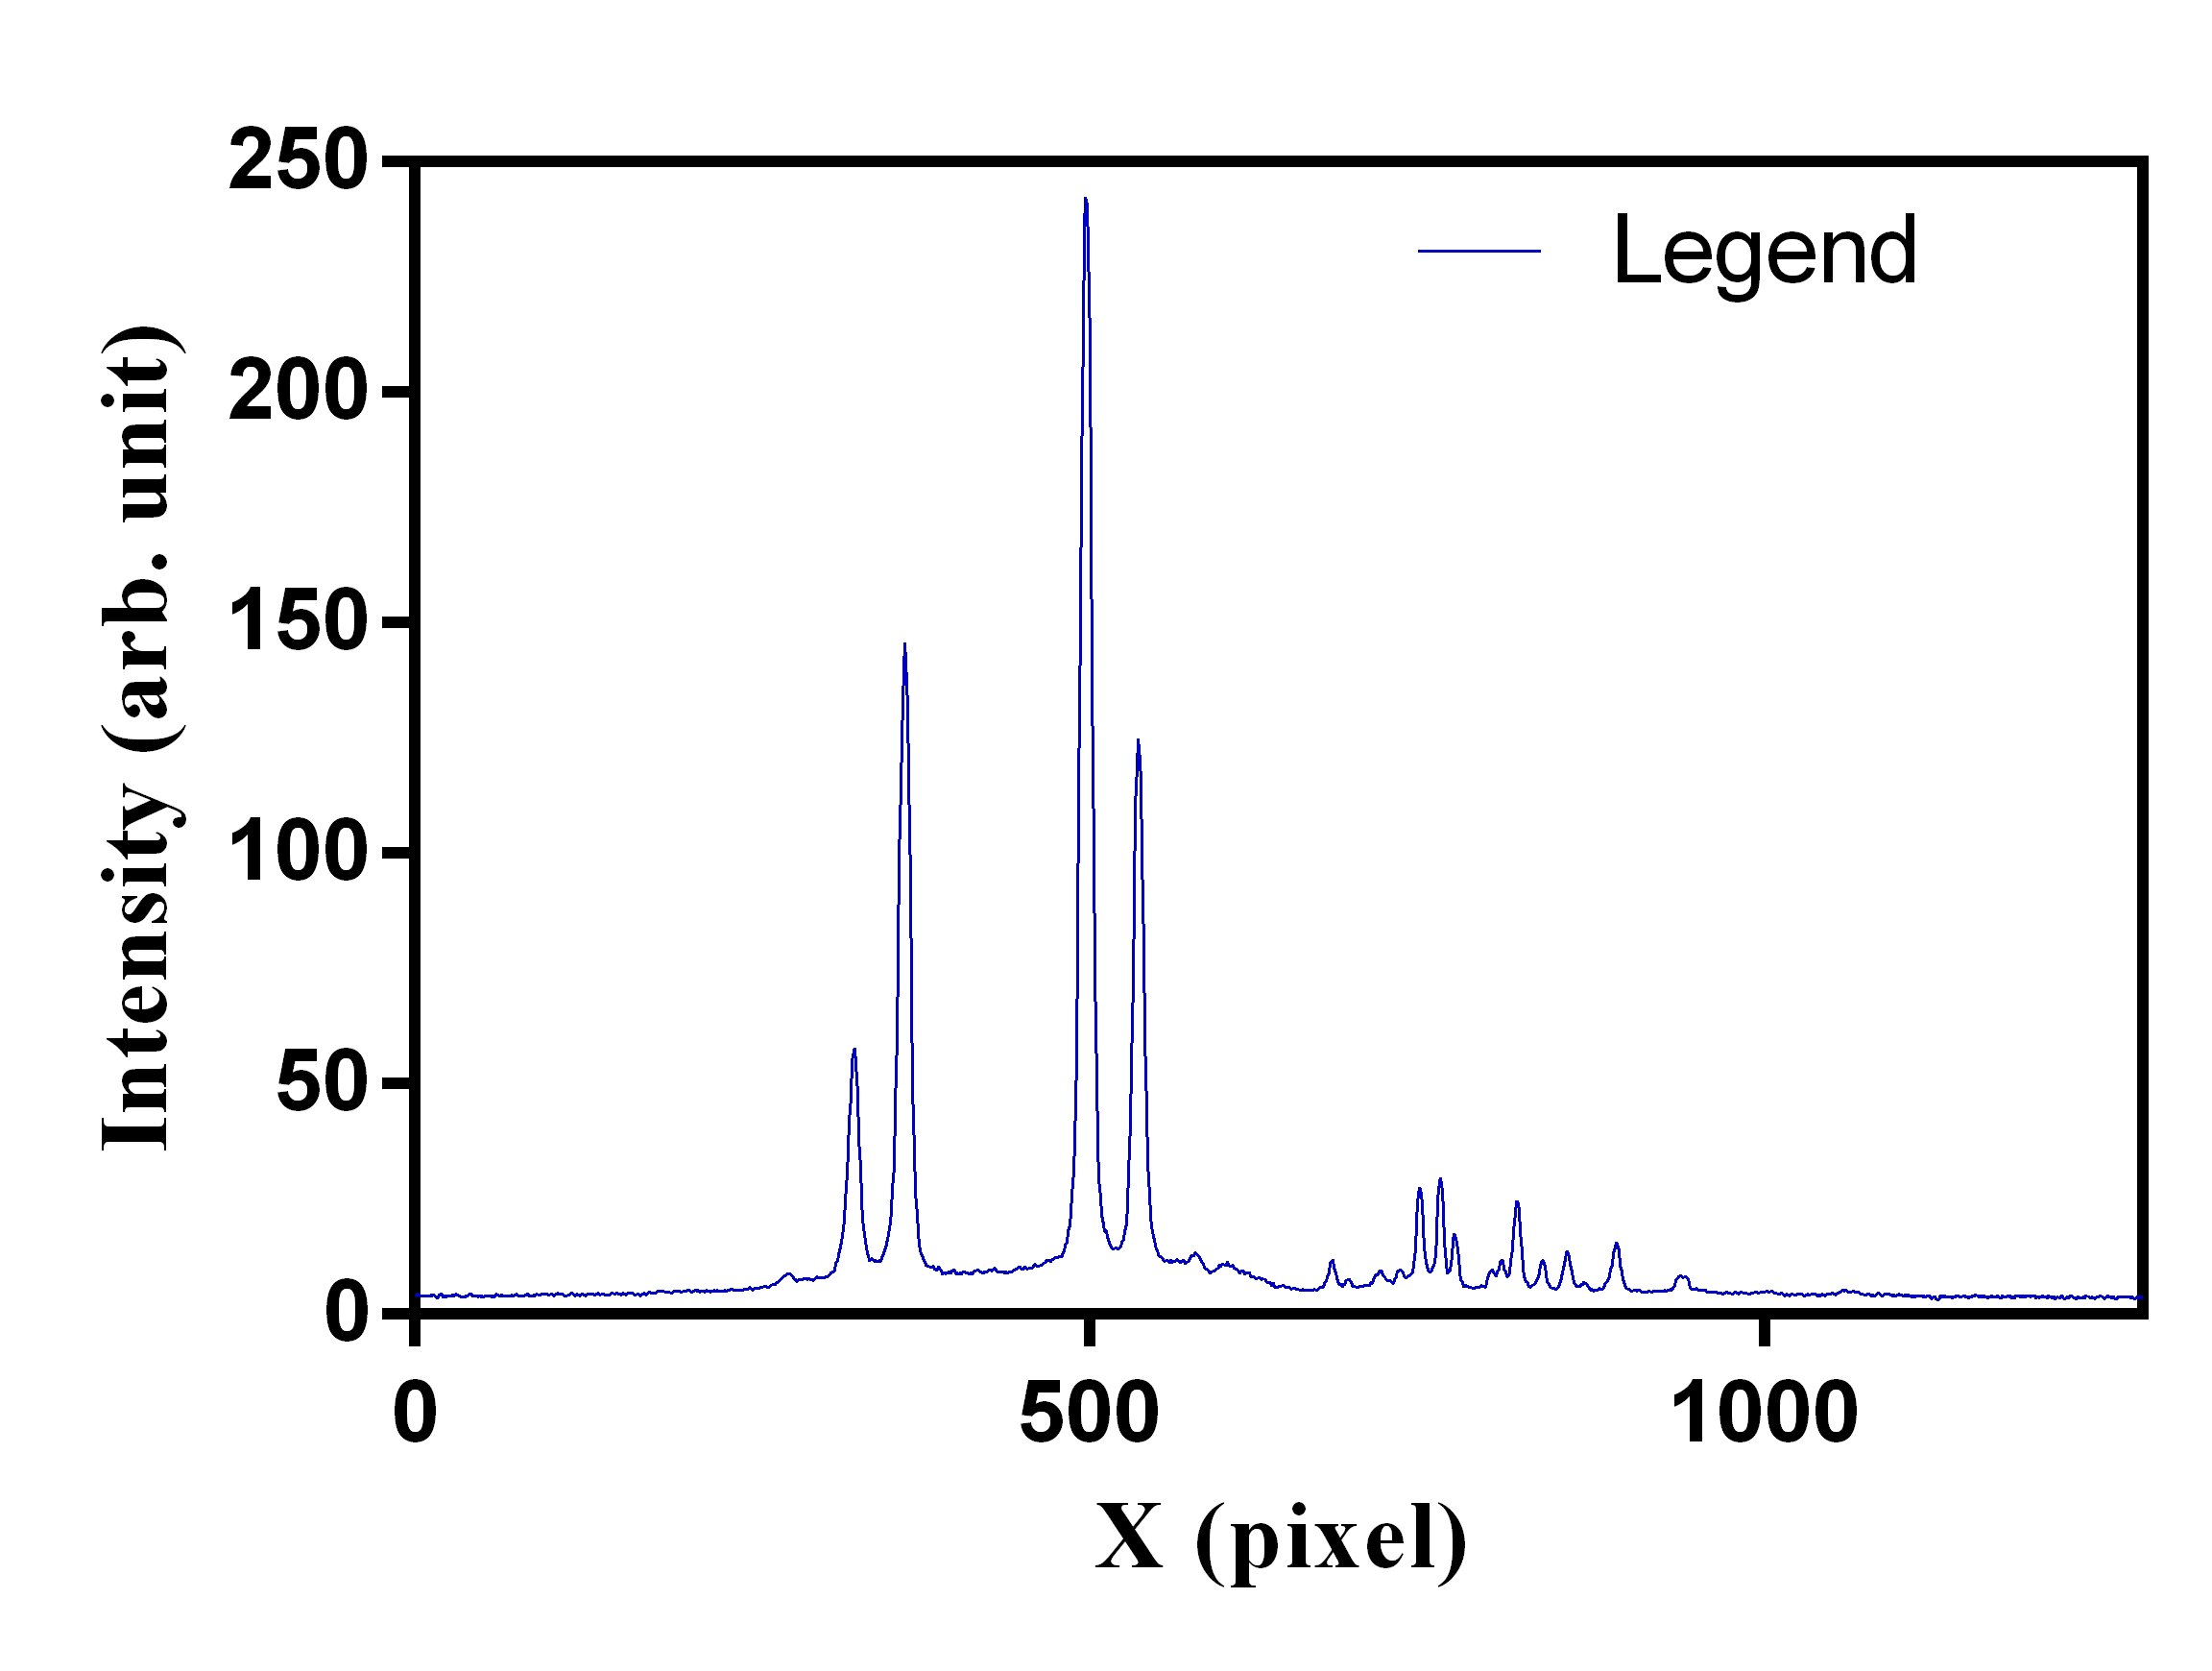
\includegraphics[width=7cm]{figures/hg_ar_4.png}
	%\caption{半高全寬與基線皆稍差}
	\caption{}
	\label{fig:d}
\end{subfigure}
\caption[汞氬燈於不同晶片的光譜表現]{汞氬燈於不同晶片下的光譜表現 (a)優良晶片光譜表現(b)半高全寬較寬(c)基線較高(d)半高全寬與基線皆稍差}
\label{fig:all}
\end{figure} 
由於汞氬燈之氬燈區光譜複雜且強度極低,對於量化判定相當困難,因此僅以汞燈區的波形表現判定,並將主要目標著重於判別基線是否升高,而晶片於較高波長時波形表現的優劣將以白光波形作為判定標準。\par
量化判定標準主要有汞氬燈之基線RMSE與半高全寬之RMSE,基線RMSE越大表示該晶片之基線升高程度越大,半高全寬之RMSE越大則代表該晶片解析度越差。量化判定需先將汞氬燈之汞燈區光譜數據透過3.5.1章所提到的分區方法分區並對各區域做勞倫茲擬合,並以小波轉換法求出基線,最後再將勞倫茲轉換後波形做基線補償得出結果,晶片間基線與波形優劣的差異如圖\ref{fig:all1}. 與圖\ref{fig:all2}. 所示。
\begin{figure}[H]
	\vspace{0.8cm}
	\centering
	\begin{subfigure}[fig nice]{0.49\textwidth}
		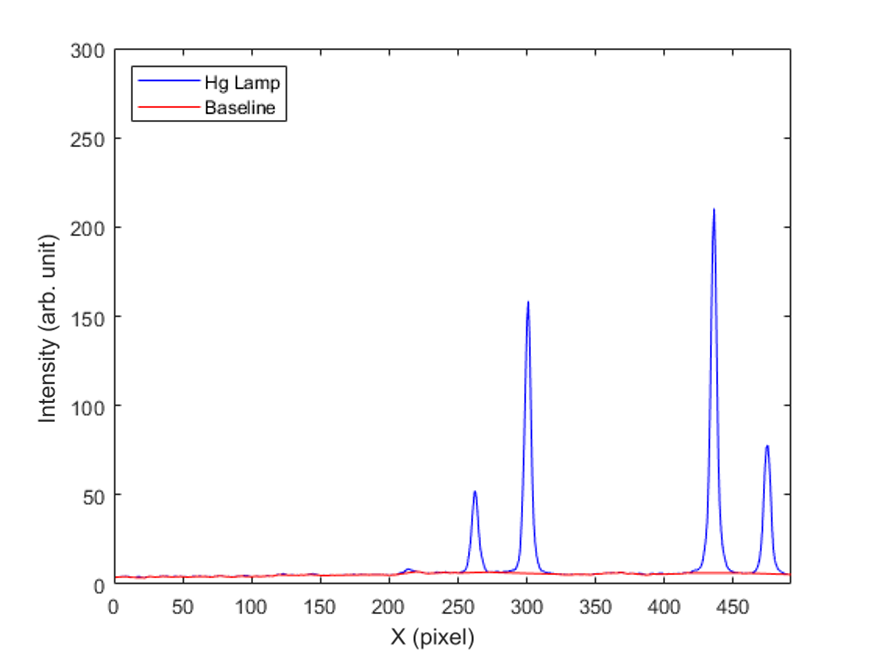
\includegraphics[width=7cm]{figures/nice_hg_base.png}
		\caption{}
		%\caption{基線表現優良晶片之汞燈光譜}
		\label{fig:a11}
	\end{subfigure}
	\begin{subfigure}[fig nice]{0.49\textwidth}
		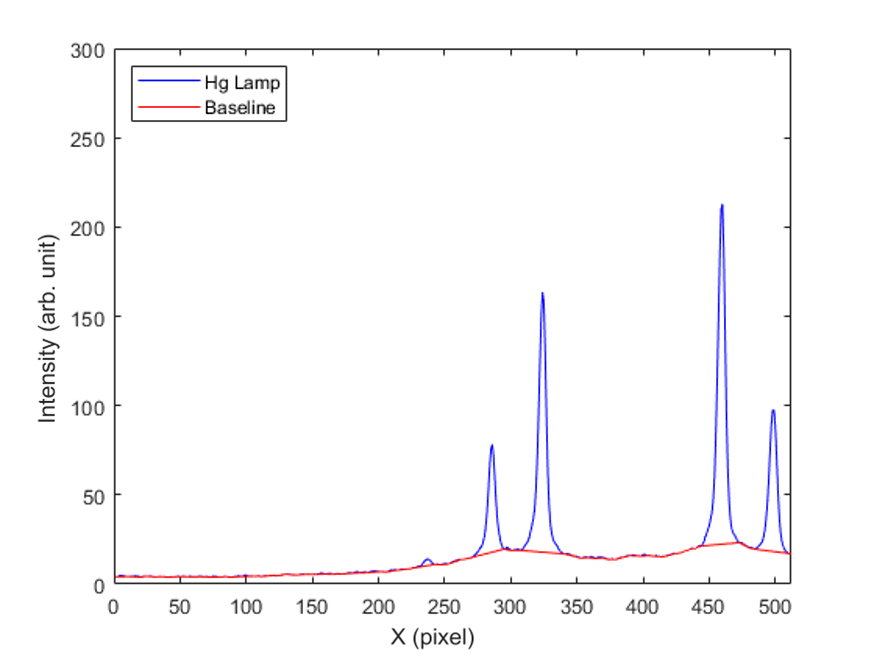
\includegraphics[width=7cm]{figures/badbase_hg_base.png}
		\caption{}
		%\caption{基線表現較差晶片之汞燈光譜}
		\label{fig:b12}
	\end{subfigure}
\begin{subfigure}[fig nice]{0.49\textwidth}
	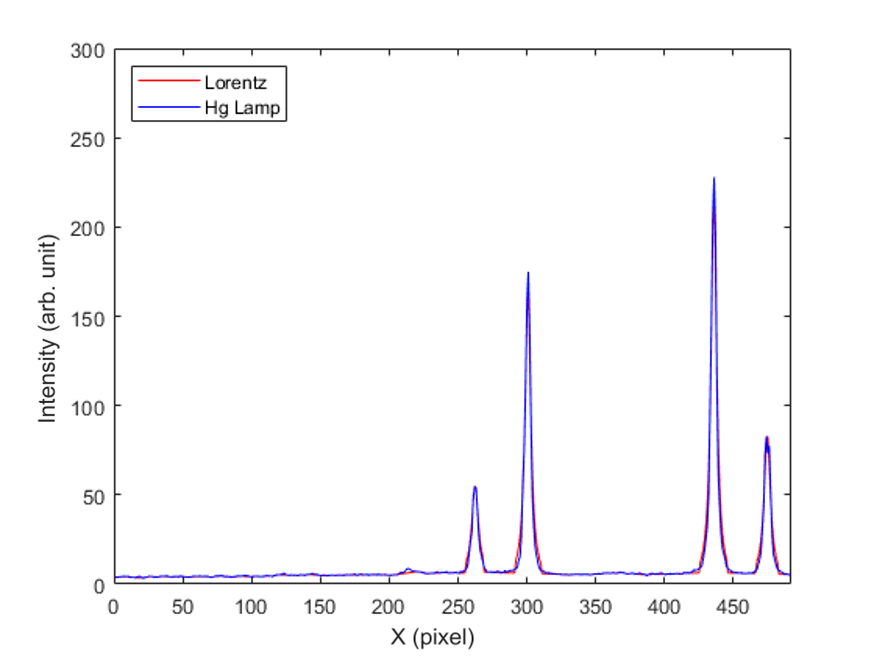
\includegraphics[width=7cm]{figures/nice_hg_lorentz.png}
	\caption{}
	%\caption{基線優良晶片勞倫茲擬合與基線補償結果}
	\label{fig:a13}
\end{subfigure}
\begin{subfigure}[fig nice]{0.49\textwidth}
	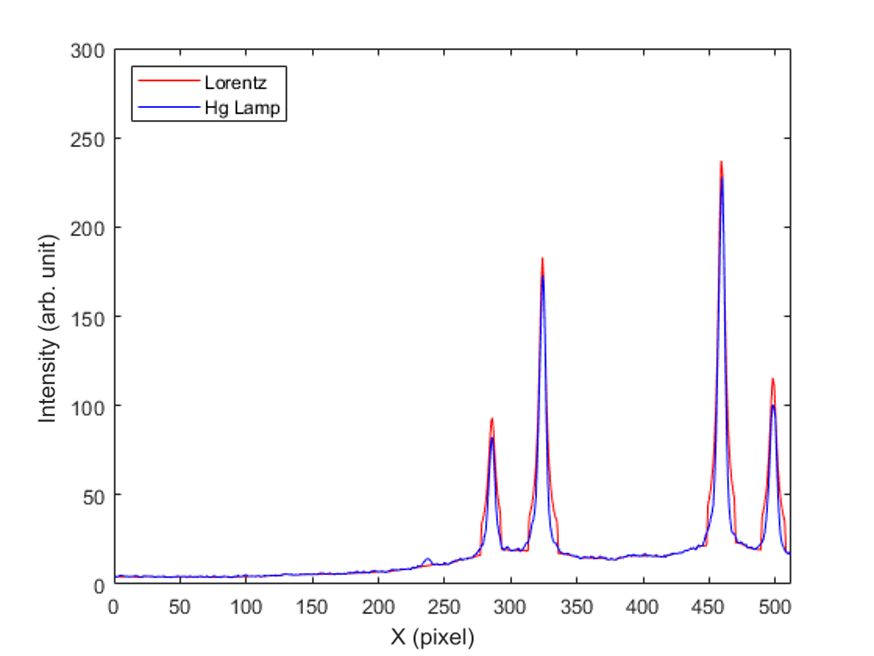
\includegraphics[width=7cm]{figures/badbase_hg_lorentz.png}
	\caption{}
	%\caption{基線較差晶片勞倫茲擬合與基線補償結果}
	\label{fig:b14}
\end{subfigure}
	\caption[波形優良但基線不佳之晶片比較]{波形優良但基線不佳之晶片比較 (a)基線表現優良晶片之汞燈光譜(b)基線表現較差晶片之汞燈光譜(c)基線優良晶片勞倫茲擬合與基線補償結果(d)基線較差晶片勞倫茲擬合與基線補償結果}
	\label{fig:all1}
\end{figure} 
如圖\ref{fig:all1}. 所示,比較圖\ref{fig:a11}. 與圖\ref{fig:b12}. 可看出圖\ref{fig:b12}. 晶片的基線升高現象相當嚴重,因此基線判定對於一個晶片的性能良好與否至關重要,而由圖\ref{fig:a13}. 與圖\ref{fig:b14}. 中可以看出性能優良的晶片,不僅基線穩定且逼近於零,在勞倫茲擬合並且基線補償後的半高全寬與波形表現皆非常優良。
\begin{figure}[H]
	\centering
	\begin{subfigure}[fig nice]{0.49\textwidth}
		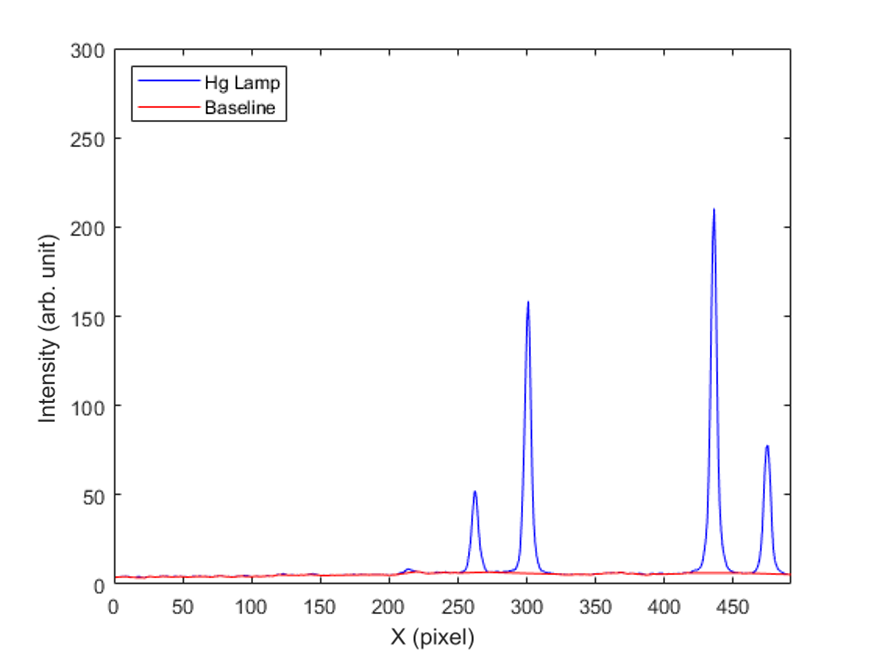
\includegraphics[width=7cm]{figures/nice_hg_base.png}
		\caption{}
		%\caption{波形優良之晶片基線表現}
		\label{fig:a21}
	\end{subfigure}
	\begin{subfigure}[fig nice]{0.49\textwidth}
		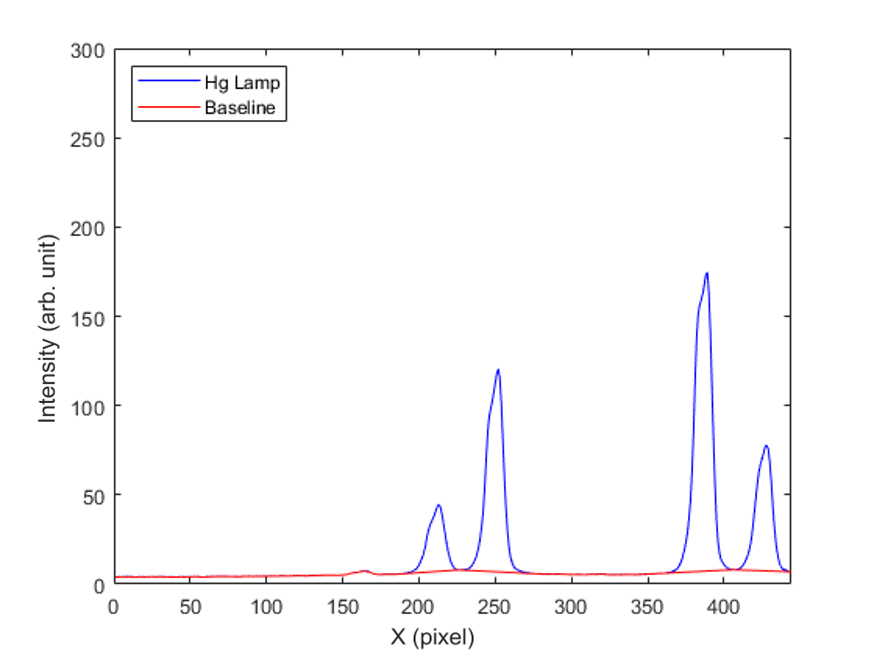
\includegraphics[width=7cm]{figures/bad_hg_base.png}
		\caption{}
		%\caption{波形較差之晶片基線表現}
		\label{fig:b22}
	\end{subfigure}
\begin{subfigure}[fig nice]{0.49\textwidth}
	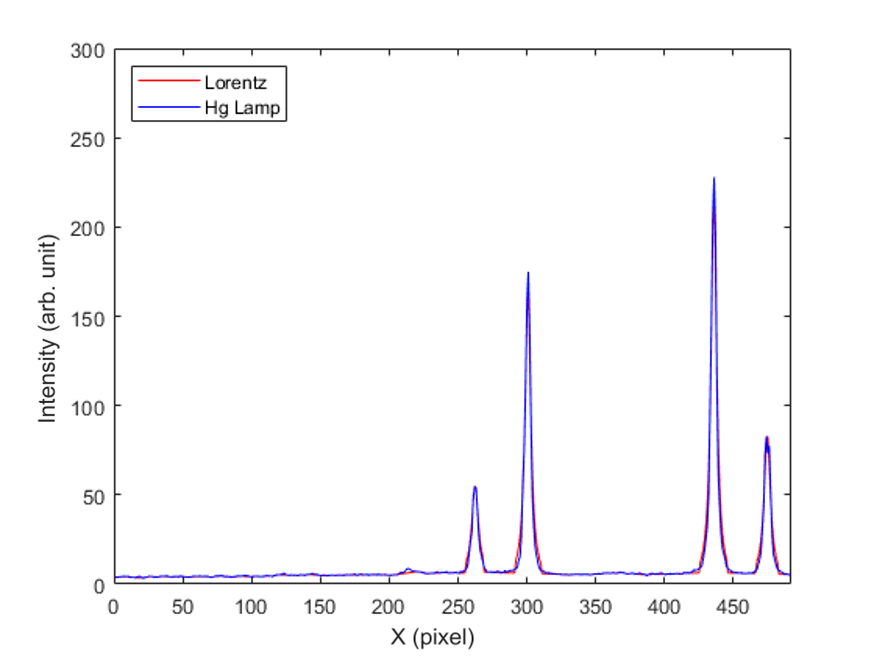
\includegraphics[width=7cm]{figures/nice_hg_lorentz.png}
	\caption{}
	%\caption{波形優良晶片勞倫茲擬合與基線補償結果}
	\label{fig:a23}
\end{subfigure}
\begin{subfigure}[fig nice]{0.49\textwidth}
	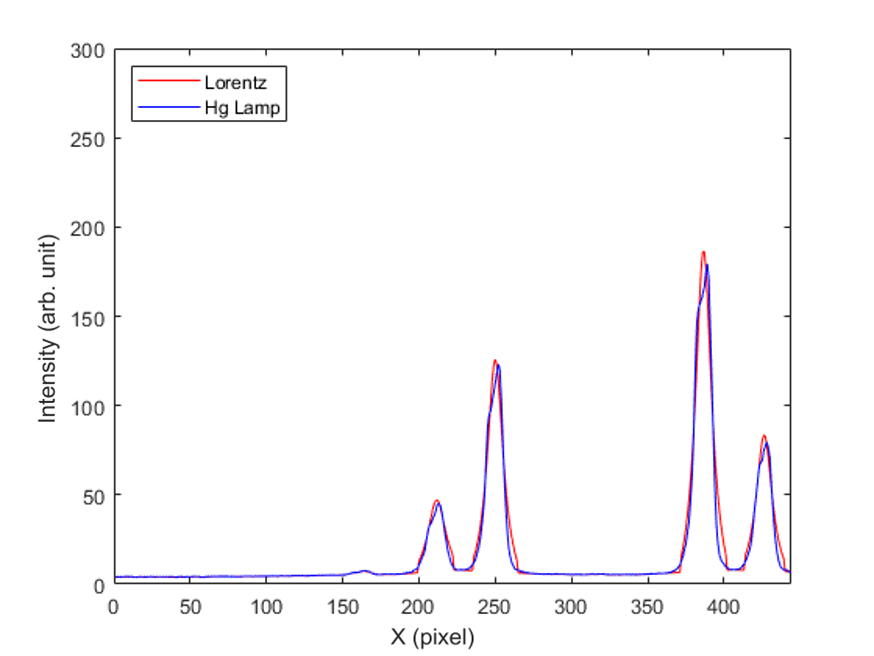
\includegraphics[width=7cm]{figures/bad_hg_lorentz.png}
	\caption{}
	%\caption{波形較差晶片勞倫茲擬合與基線補償結果}
	\label{fig:b24}
\end{subfigure}
	\caption[基線優良但波形不佳之晶片比較]{基線優良但波形不佳之晶片比較 (a)波形優良之晶片基線表現(b)波形較差之晶片基線表現(c)波形優良晶片勞倫茲擬合與基線補償結果(d)波形較差晶片勞倫茲擬合與基線補償結果}
	\label{fig:all2}
\end{figure}  
如圖\ref{fig:all2}. 所示,由圖\ref{fig:a21}. 與圖\ref{fig:b22}. 比較可看出雖然兩個晶片的基線升高現象都非常輕微,但由圖\ref{fig:a23}. 與圖\ref{fig:b24}. 中可以看出勞倫茲擬合後圖\ref{fig:b24}. 之半高全寬相當大,因此不僅需將基線升高現象做為晶片效能優良與否判斷,勞倫茲擬合後的半高全寬也是晶片效能的重要參考點。

\subsection{白光LED波形量化判定}
不同於汞氬燈光譜波形的多個獨立錐狀,且峰與峰間有無信號區,白光光譜如圖\ref{白光LED光譜}. 所示,橫跨幾乎所有可見光波段,又因其光譜波形連續不中斷,因此比起汞氬燈更能體現出晶片的光譜表現。\par
白光LED為藍光晶粒激發黃色螢光而產生白光,因此藍光與黃光相互影響作用,且因白光連續不中斷,造成難以判定是否有基線升高現象,而基線已於汞氬燈時判定,因此白光LED量化判定著重於判定整個可見光波段中光譜波形表現。\par
\begin{figure}[H] %H为当前位置,!htb为忽略美学标准,htbp为浮动图形
	\centering %图片居中
	\vspace{0.8cm}
	\setlength{\abovecaptionskip}{0.cm}
	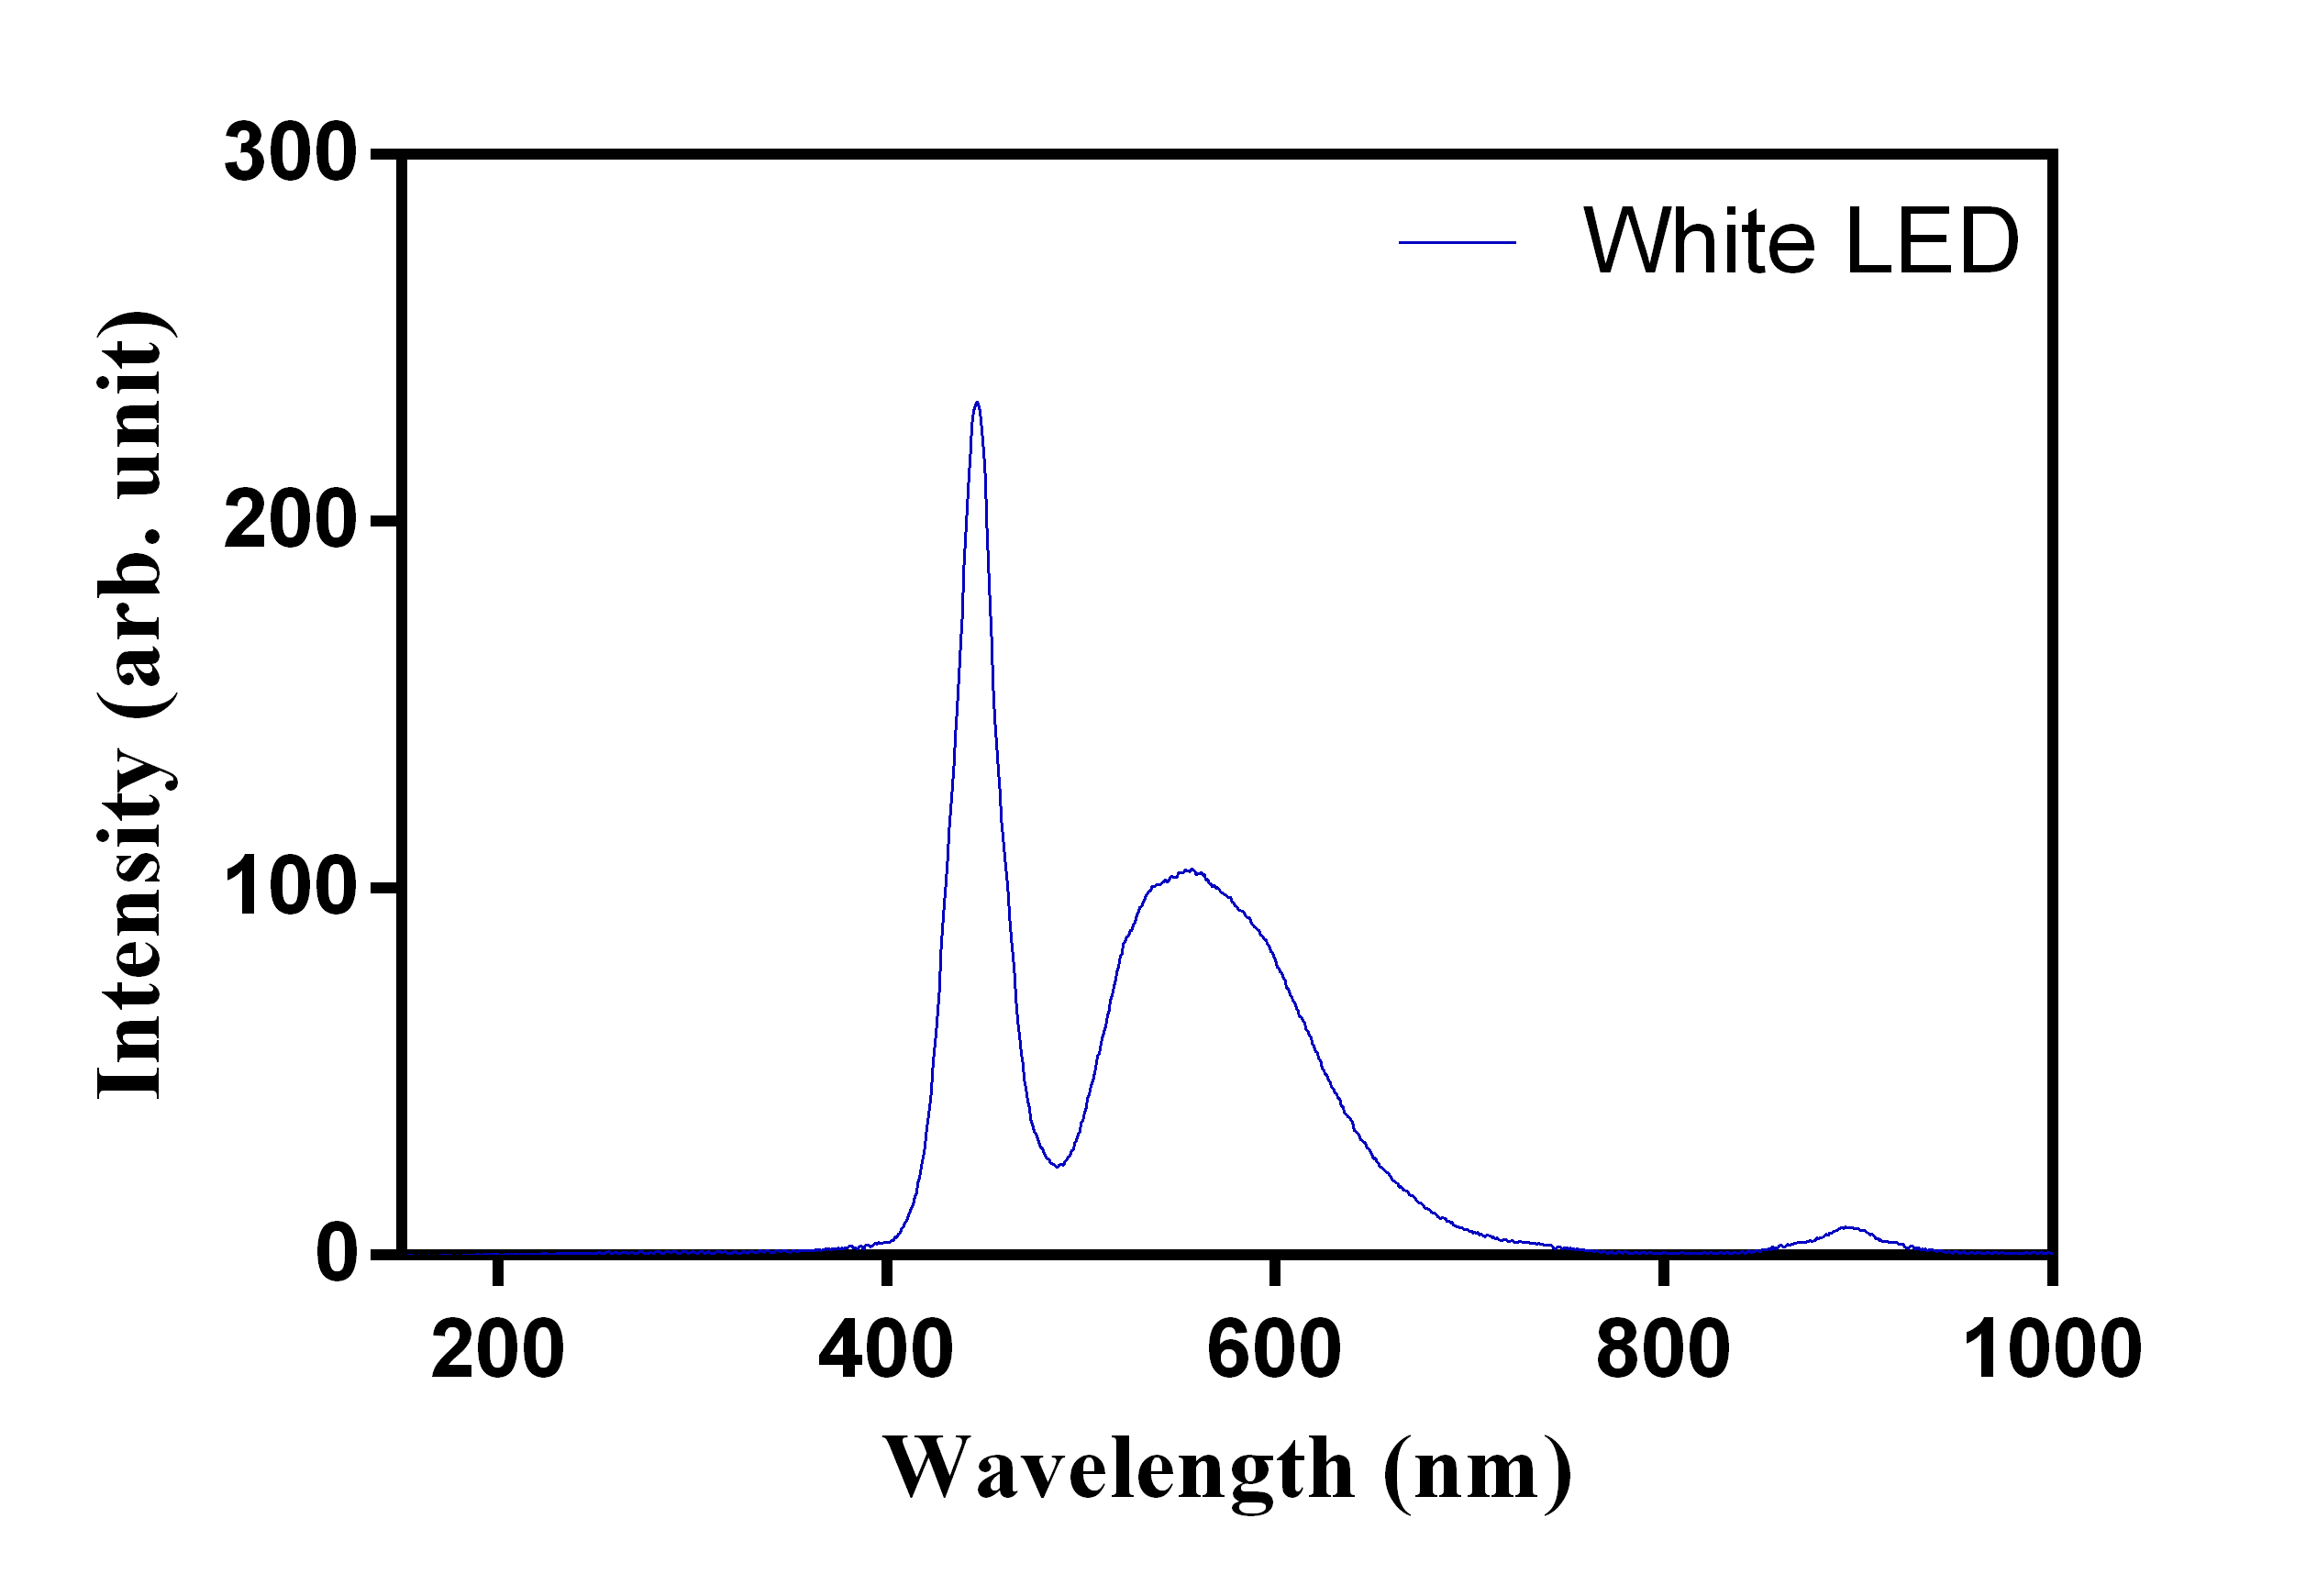
\includegraphics[width=\textwidth]{figures/White_wavelenght.png} %插入图片,[]中设置图片大小,{}中是图片文件名
	\caption{白光LED光譜} %最终文档中希望显示的图片标题
	\label{白光LED光譜} %用于文内引用的标签
\end{figure}
白光LED模型擬合如表\ref{光源介紹表}. 所示,需同時以兩種不同模型表示。本文先將光譜拆為兩段分析,藍光LED晶粒產生的光譜為躍遷光譜,躍遷光譜極逼近於勞倫茲函數模型,而受激發而發亮的黃色螢光粉則逼近於高斯函數模型,首先將白光LED以3.5.1章所提的分區方法將白光數據切割,並將第一區間的藍光光譜以勞倫茲模型擬合,如圖\ref{藍光區域以勞倫茲模型擬合結果}. 所示。
\begin{figure}[H] %H为当前位置,!htb为忽略美学标准,htbp为浮动图形
	\centering %图片居中
	%\setlength{\abovecaptionskip}{1cm}
	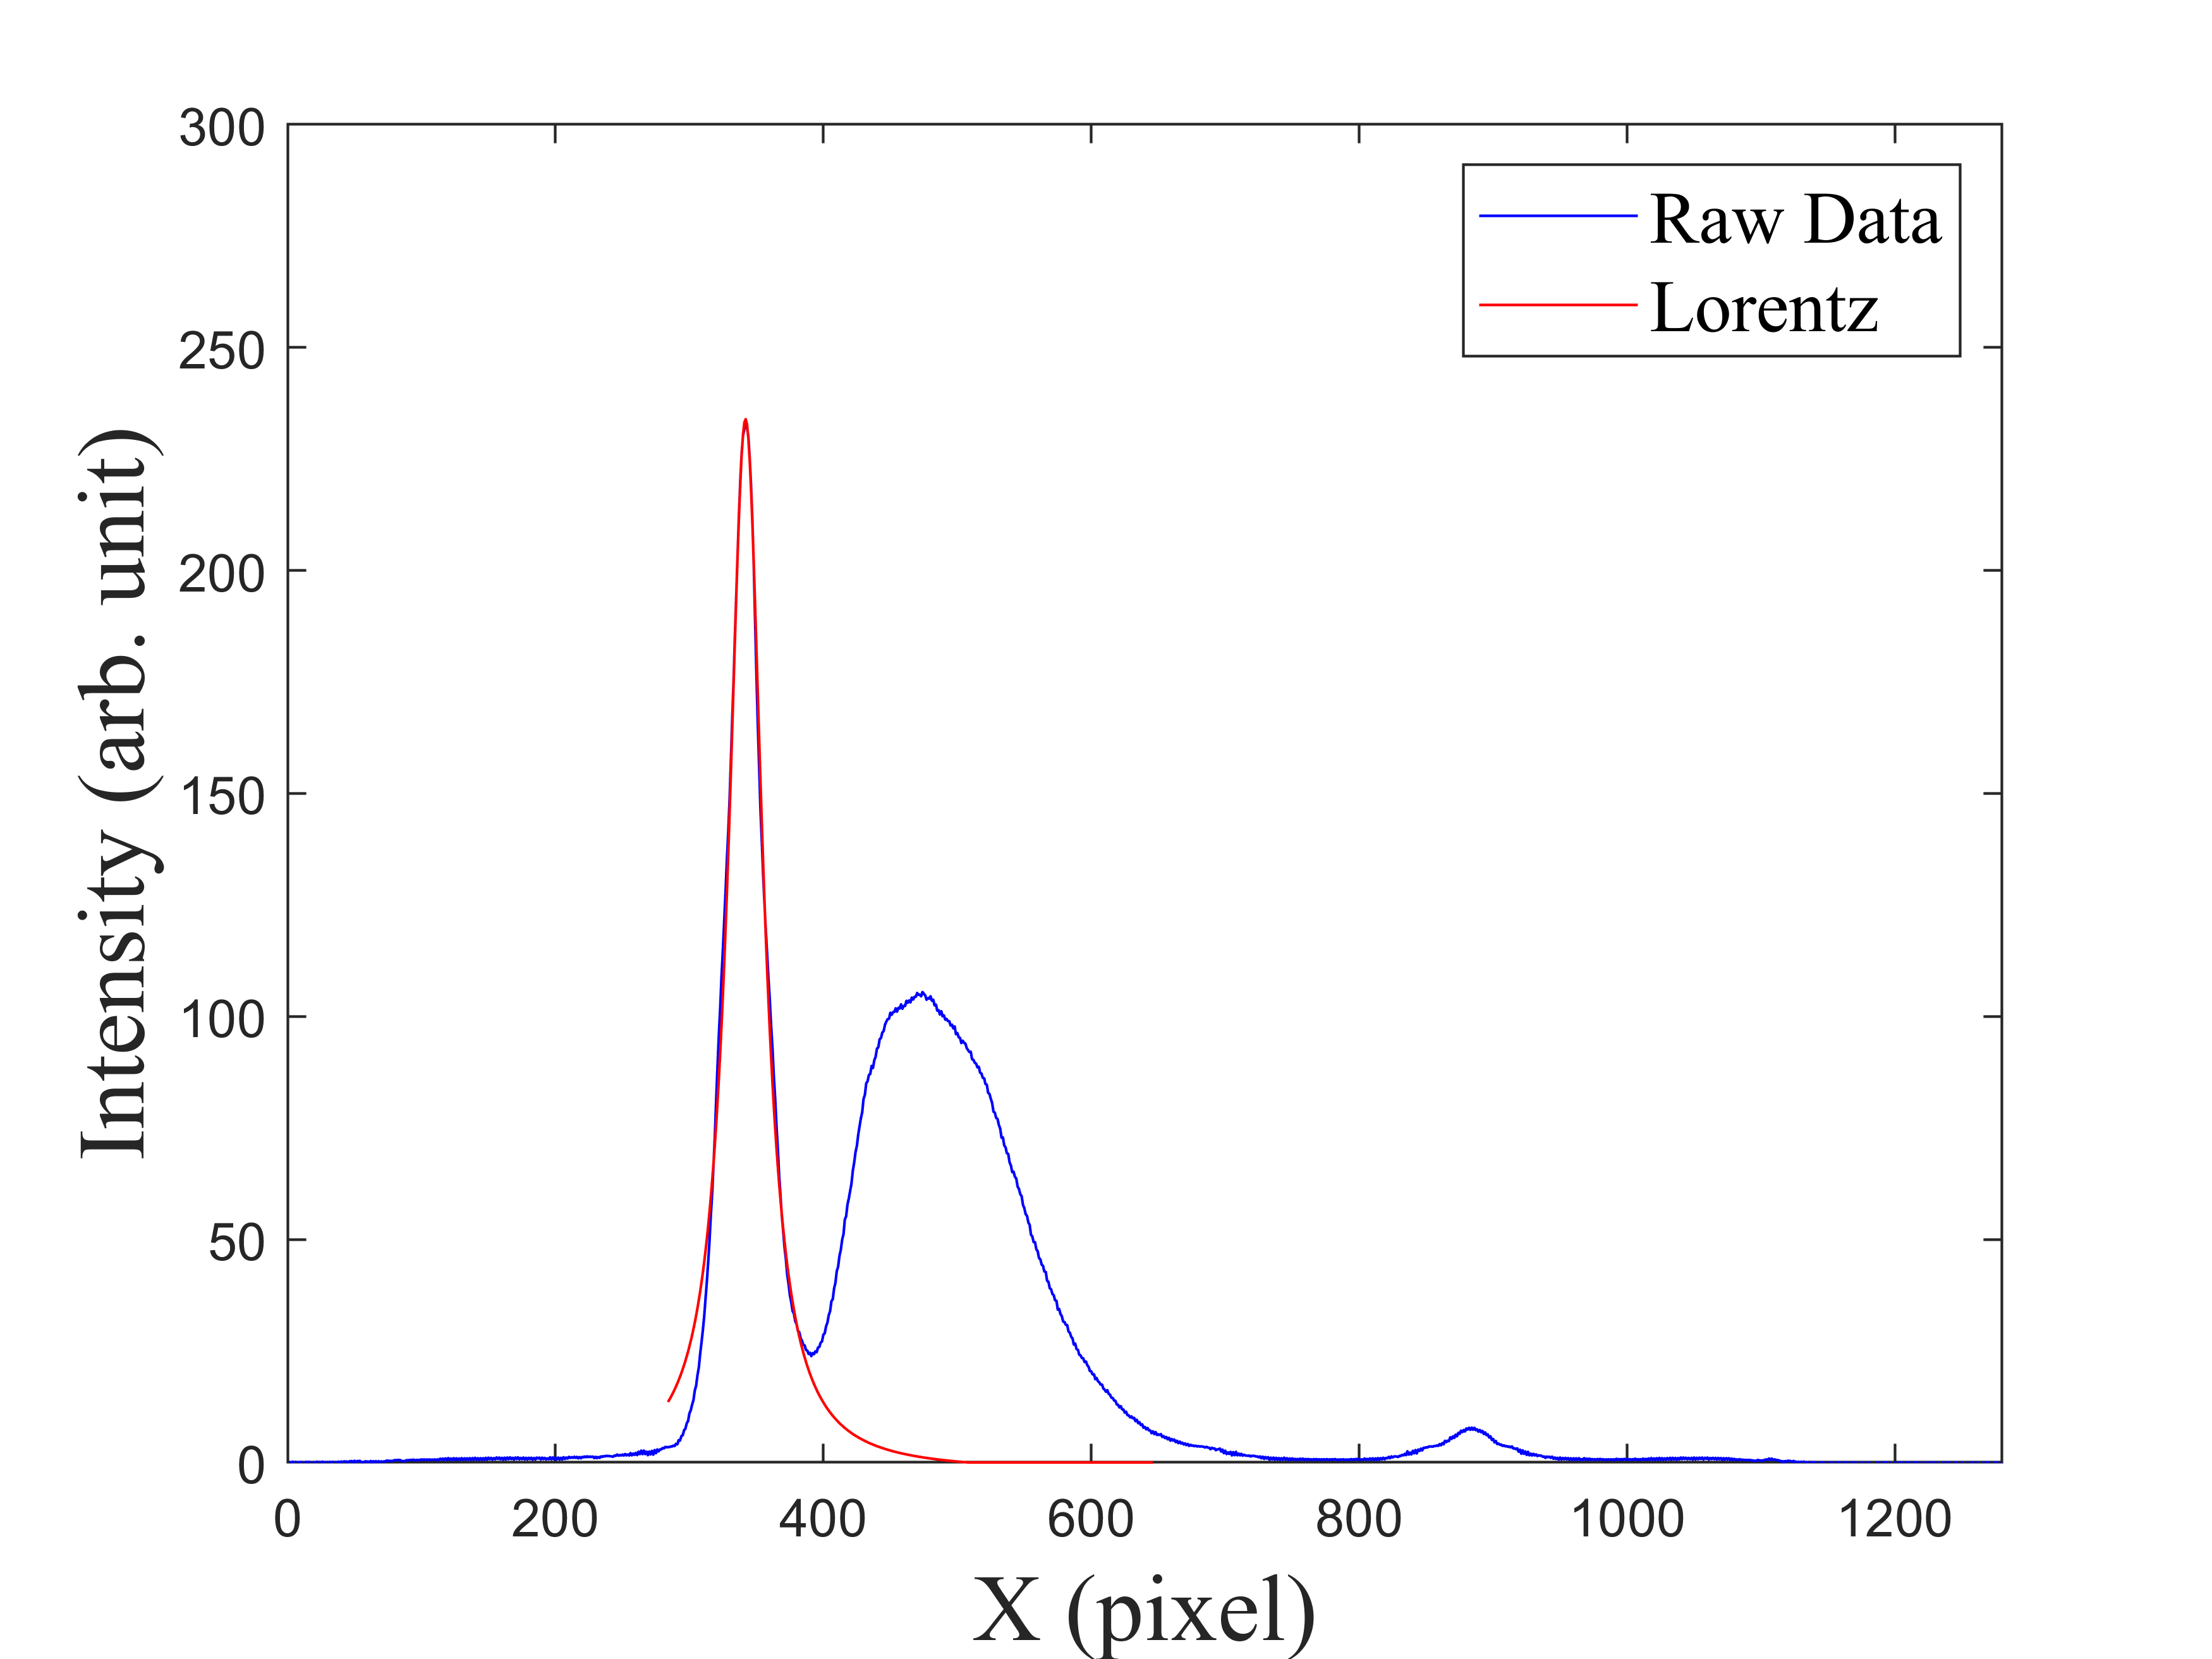
\includegraphics[width=16cm]{figures/white_lorentz.png} %插入图片,[]中设置图片大小,{}中是图片文件名
	\caption{藍光區域以勞倫茲模型擬合結果} %最终文档中希望显示的图片标题
	\label{藍光區域以勞倫茲模型擬合結果} %用于文内引用的标签
\end{figure}
由於藍光波形與黃色螢光波形相互影響作用,而藍光因強度較螢光強上許多,因此受黃色螢光影響較小,可以直接以勞倫茲模型擬合逼近,而因黃色螢光較弱,所以受到藍光的影響,造成黃色螢光前端的強度攀升區域的波形與藍光耦合,若直接以高斯模型擬合將會產生較大誤差。\par
圖\ref{藍光區域以勞倫茲模型擬合結果}. 為透過擬合得出勞倫茲方程式後,將像素帶入方程式估算出藍光光譜的延伸波形。將白光光譜扣除藍光對於後方螢光區域的影響後,螢光區的光譜就可以使用高斯函數逼近,逼近後結果如圖\ref{螢光區域以高斯模型擬合結果}. 所示。
\begin{figure}[H] %H为当前位置,!htb为忽略美学标准,htbp为浮动图形
	\centering %图片居中
	%\setlength{\abovecaptionskip}{1cm}
	\includegraphics[width=16cm]{figures/white_gaussian.png} %插入图片,[]中设置图片大小,{}中是图片文件名
	\caption{螢光區域以高斯模型擬合結果} %最终文档中希望显示的图片标题
	\label{螢光區域以高斯模型擬合結果} %用于文内引用的标签
\end{figure}
兩區域數據處理並擬合後,將圖\ref{螢光區域以高斯模型擬合結果}. 中的高斯模型函數往前延伸並求出與勞倫茲函數模型的交點,並以此點做為結合點將兩模型組合為白光LED光譜的理想參考波形。\par
圖\ref{雙模型擬合結果}. 為實際對晶片以白光LED做量化判定的結果,並標示透過兩模型擬合後所得出的半高全寬與原始數據對參考波形的總體RMSE,此兩項數據可提供使用者做為晶片優劣的量化判定值。
\begin{figure}[H] %H为当前位置,!htb为忽略美学标准,htbp为浮动图形
	\centering %图片居中
	%\setlength{\abovecaptionskip}{1cm}
	\includegraphics[width=\textwidth]{figures/20C4-203-D1.png} %插入图片,[]中设置图片大小,{}中是图片文件名
	\caption{雙模型擬合結果} %最终文档中希望显示的图片标题
	\label{雙模型擬合結果} %用于文内引用的标签
\end{figure}